\documentclass[]{book}
\usepackage{lmodern}
\usepackage{amssymb,amsmath}
\usepackage{ifxetex,ifluatex}
\usepackage{fixltx2e} % provides \textsubscript
\ifnum 0\ifxetex 1\fi\ifluatex 1\fi=0 % if pdftex
  \usepackage[T1]{fontenc}
  \usepackage[utf8]{inputenc}
\else % if luatex or xelatex
  \ifxetex
    \usepackage{mathspec}
  \else
    \usepackage{fontspec}
  \fi
  \defaultfontfeatures{Ligatures=TeX,Scale=MatchLowercase}
\fi
% use upquote if available, for straight quotes in verbatim environments
\IfFileExists{upquote.sty}{\usepackage{upquote}}{}
% use microtype if available
\IfFileExists{microtype.sty}{%
\usepackage{microtype}
\UseMicrotypeSet[protrusion]{basicmath} % disable protrusion for tt fonts
}{}
\usepackage[margin=1in]{geometry}
\usepackage{hyperref}
\hypersetup{unicode=true,
            pdftitle={Notes for Teaching an Undergraduate Statistics Using fastR},
            pdfauthor={Bradley Warner},
            pdfborder={0 0 0},
            breaklinks=true}
\urlstyle{same}  % don't use monospace font for urls
\usepackage{natbib}
\bibliographystyle{apalike}
\usepackage{color}
\usepackage{fancyvrb}
\newcommand{\VerbBar}{|}
\newcommand{\VERB}{\Verb[commandchars=\\\{\}]}
\DefineVerbatimEnvironment{Highlighting}{Verbatim}{commandchars=\\\{\}}
% Add ',fontsize=\small' for more characters per line
\usepackage{framed}
\definecolor{shadecolor}{RGB}{248,248,248}
\newenvironment{Shaded}{\begin{snugshade}}{\end{snugshade}}
\newcommand{\KeywordTok}[1]{\textcolor[rgb]{0.13,0.29,0.53}{\textbf{#1}}}
\newcommand{\DataTypeTok}[1]{\textcolor[rgb]{0.13,0.29,0.53}{#1}}
\newcommand{\DecValTok}[1]{\textcolor[rgb]{0.00,0.00,0.81}{#1}}
\newcommand{\BaseNTok}[1]{\textcolor[rgb]{0.00,0.00,0.81}{#1}}
\newcommand{\FloatTok}[1]{\textcolor[rgb]{0.00,0.00,0.81}{#1}}
\newcommand{\ConstantTok}[1]{\textcolor[rgb]{0.00,0.00,0.00}{#1}}
\newcommand{\CharTok}[1]{\textcolor[rgb]{0.31,0.60,0.02}{#1}}
\newcommand{\SpecialCharTok}[1]{\textcolor[rgb]{0.00,0.00,0.00}{#1}}
\newcommand{\StringTok}[1]{\textcolor[rgb]{0.31,0.60,0.02}{#1}}
\newcommand{\VerbatimStringTok}[1]{\textcolor[rgb]{0.31,0.60,0.02}{#1}}
\newcommand{\SpecialStringTok}[1]{\textcolor[rgb]{0.31,0.60,0.02}{#1}}
\newcommand{\ImportTok}[1]{#1}
\newcommand{\CommentTok}[1]{\textcolor[rgb]{0.56,0.35,0.01}{\textit{#1}}}
\newcommand{\DocumentationTok}[1]{\textcolor[rgb]{0.56,0.35,0.01}{\textbf{\textit{#1}}}}
\newcommand{\AnnotationTok}[1]{\textcolor[rgb]{0.56,0.35,0.01}{\textbf{\textit{#1}}}}
\newcommand{\CommentVarTok}[1]{\textcolor[rgb]{0.56,0.35,0.01}{\textbf{\textit{#1}}}}
\newcommand{\OtherTok}[1]{\textcolor[rgb]{0.56,0.35,0.01}{#1}}
\newcommand{\FunctionTok}[1]{\textcolor[rgb]{0.00,0.00,0.00}{#1}}
\newcommand{\VariableTok}[1]{\textcolor[rgb]{0.00,0.00,0.00}{#1}}
\newcommand{\ControlFlowTok}[1]{\textcolor[rgb]{0.13,0.29,0.53}{\textbf{#1}}}
\newcommand{\OperatorTok}[1]{\textcolor[rgb]{0.81,0.36,0.00}{\textbf{#1}}}
\newcommand{\BuiltInTok}[1]{#1}
\newcommand{\ExtensionTok}[1]{#1}
\newcommand{\PreprocessorTok}[1]{\textcolor[rgb]{0.56,0.35,0.01}{\textit{#1}}}
\newcommand{\AttributeTok}[1]{\textcolor[rgb]{0.77,0.63,0.00}{#1}}
\newcommand{\RegionMarkerTok}[1]{#1}
\newcommand{\InformationTok}[1]{\textcolor[rgb]{0.56,0.35,0.01}{\textbf{\textit{#1}}}}
\newcommand{\WarningTok}[1]{\textcolor[rgb]{0.56,0.35,0.01}{\textbf{\textit{#1}}}}
\newcommand{\AlertTok}[1]{\textcolor[rgb]{0.94,0.16,0.16}{#1}}
\newcommand{\ErrorTok}[1]{\textcolor[rgb]{0.64,0.00,0.00}{\textbf{#1}}}
\newcommand{\NormalTok}[1]{#1}
\usepackage{longtable,booktabs}
\usepackage{graphicx,grffile}
\makeatletter
\def\maxwidth{\ifdim\Gin@nat@width>\linewidth\linewidth\else\Gin@nat@width\fi}
\def\maxheight{\ifdim\Gin@nat@height>\textheight\textheight\else\Gin@nat@height\fi}
\makeatother
% Scale images if necessary, so that they will not overflow the page
% margins by default, and it is still possible to overwrite the defaults
% using explicit options in \includegraphics[width, height, ...]{}
\setkeys{Gin}{width=\maxwidth,height=\maxheight,keepaspectratio}
\IfFileExists{parskip.sty}{%
\usepackage{parskip}
}{% else
\setlength{\parindent}{0pt}
\setlength{\parskip}{6pt plus 2pt minus 1pt}
}
\setlength{\emergencystretch}{3em}  % prevent overfull lines
\providecommand{\tightlist}{%
  \setlength{\itemsep}{0pt}\setlength{\parskip}{0pt}}
\setcounter{secnumdepth}{5}
% Redefines (sub)paragraphs to behave more like sections
\ifx\paragraph\undefined\else
\let\oldparagraph\paragraph
\renewcommand{\paragraph}[1]{\oldparagraph{#1}\mbox{}}
\fi
\ifx\subparagraph\undefined\else
\let\oldsubparagraph\subparagraph
\renewcommand{\subparagraph}[1]{\oldsubparagraph{#1}\mbox{}}
\fi

%%% Use protect on footnotes to avoid problems with footnotes in titles
\let\rmarkdownfootnote\footnote%
\def\footnote{\protect\rmarkdownfootnote}

%%% Change title format to be more compact
\usepackage{titling}

% Create subtitle command for use in maketitle
\newcommand{\subtitle}[1]{
  \posttitle{
    \begin{center}\large#1\end{center}
    }
}

\setlength{\droptitle}{-2em}
  \title{Notes for Teaching an Undergraduate Statistics Using fastR}
  \pretitle{\vspace{\droptitle}\centering\huge}
  \posttitle{\par}
  \author{Bradley Warner}
  \preauthor{\centering\large\emph}
  \postauthor{\par}
  \predate{\centering\large\emph}
  \postdate{\par}
  \date{2018-01-31}

\usepackage{booktabs}
\usepackage{amsthm}
\makeatletter
\def\thm@space@setup{%
  \thm@preskip=8pt plus 2pt minus 4pt
  \thm@postskip=\thm@preskip
}
\makeatother

\usepackage{amsthm}
\newtheorem{theorem}{Theorem}[chapter]
\newtheorem{lemma}{Lemma}[chapter]
\theoremstyle{definition}
\newtheorem{definition}{Definition}[chapter]
\newtheorem{corollary}{Corollary}[chapter]
\newtheorem{proposition}{Proposition}[chapter]
\theoremstyle{definition}
\newtheorem{example}{Example}[chapter]
\theoremstyle{definition}
\newtheorem{exercise}{Exercise}[chapter]
\theoremstyle{remark}
\newtheorem*{remark}{Remark}
\newtheorem*{solution}{Solution}
\begin{document}
\maketitle

{
\setcounter{tocdepth}{1}
\tableofcontents
}
\chapter*{Preface}\label{preface}
\addcontentsline{toc}{chapter}{Preface}

\begin{figure}
\centering
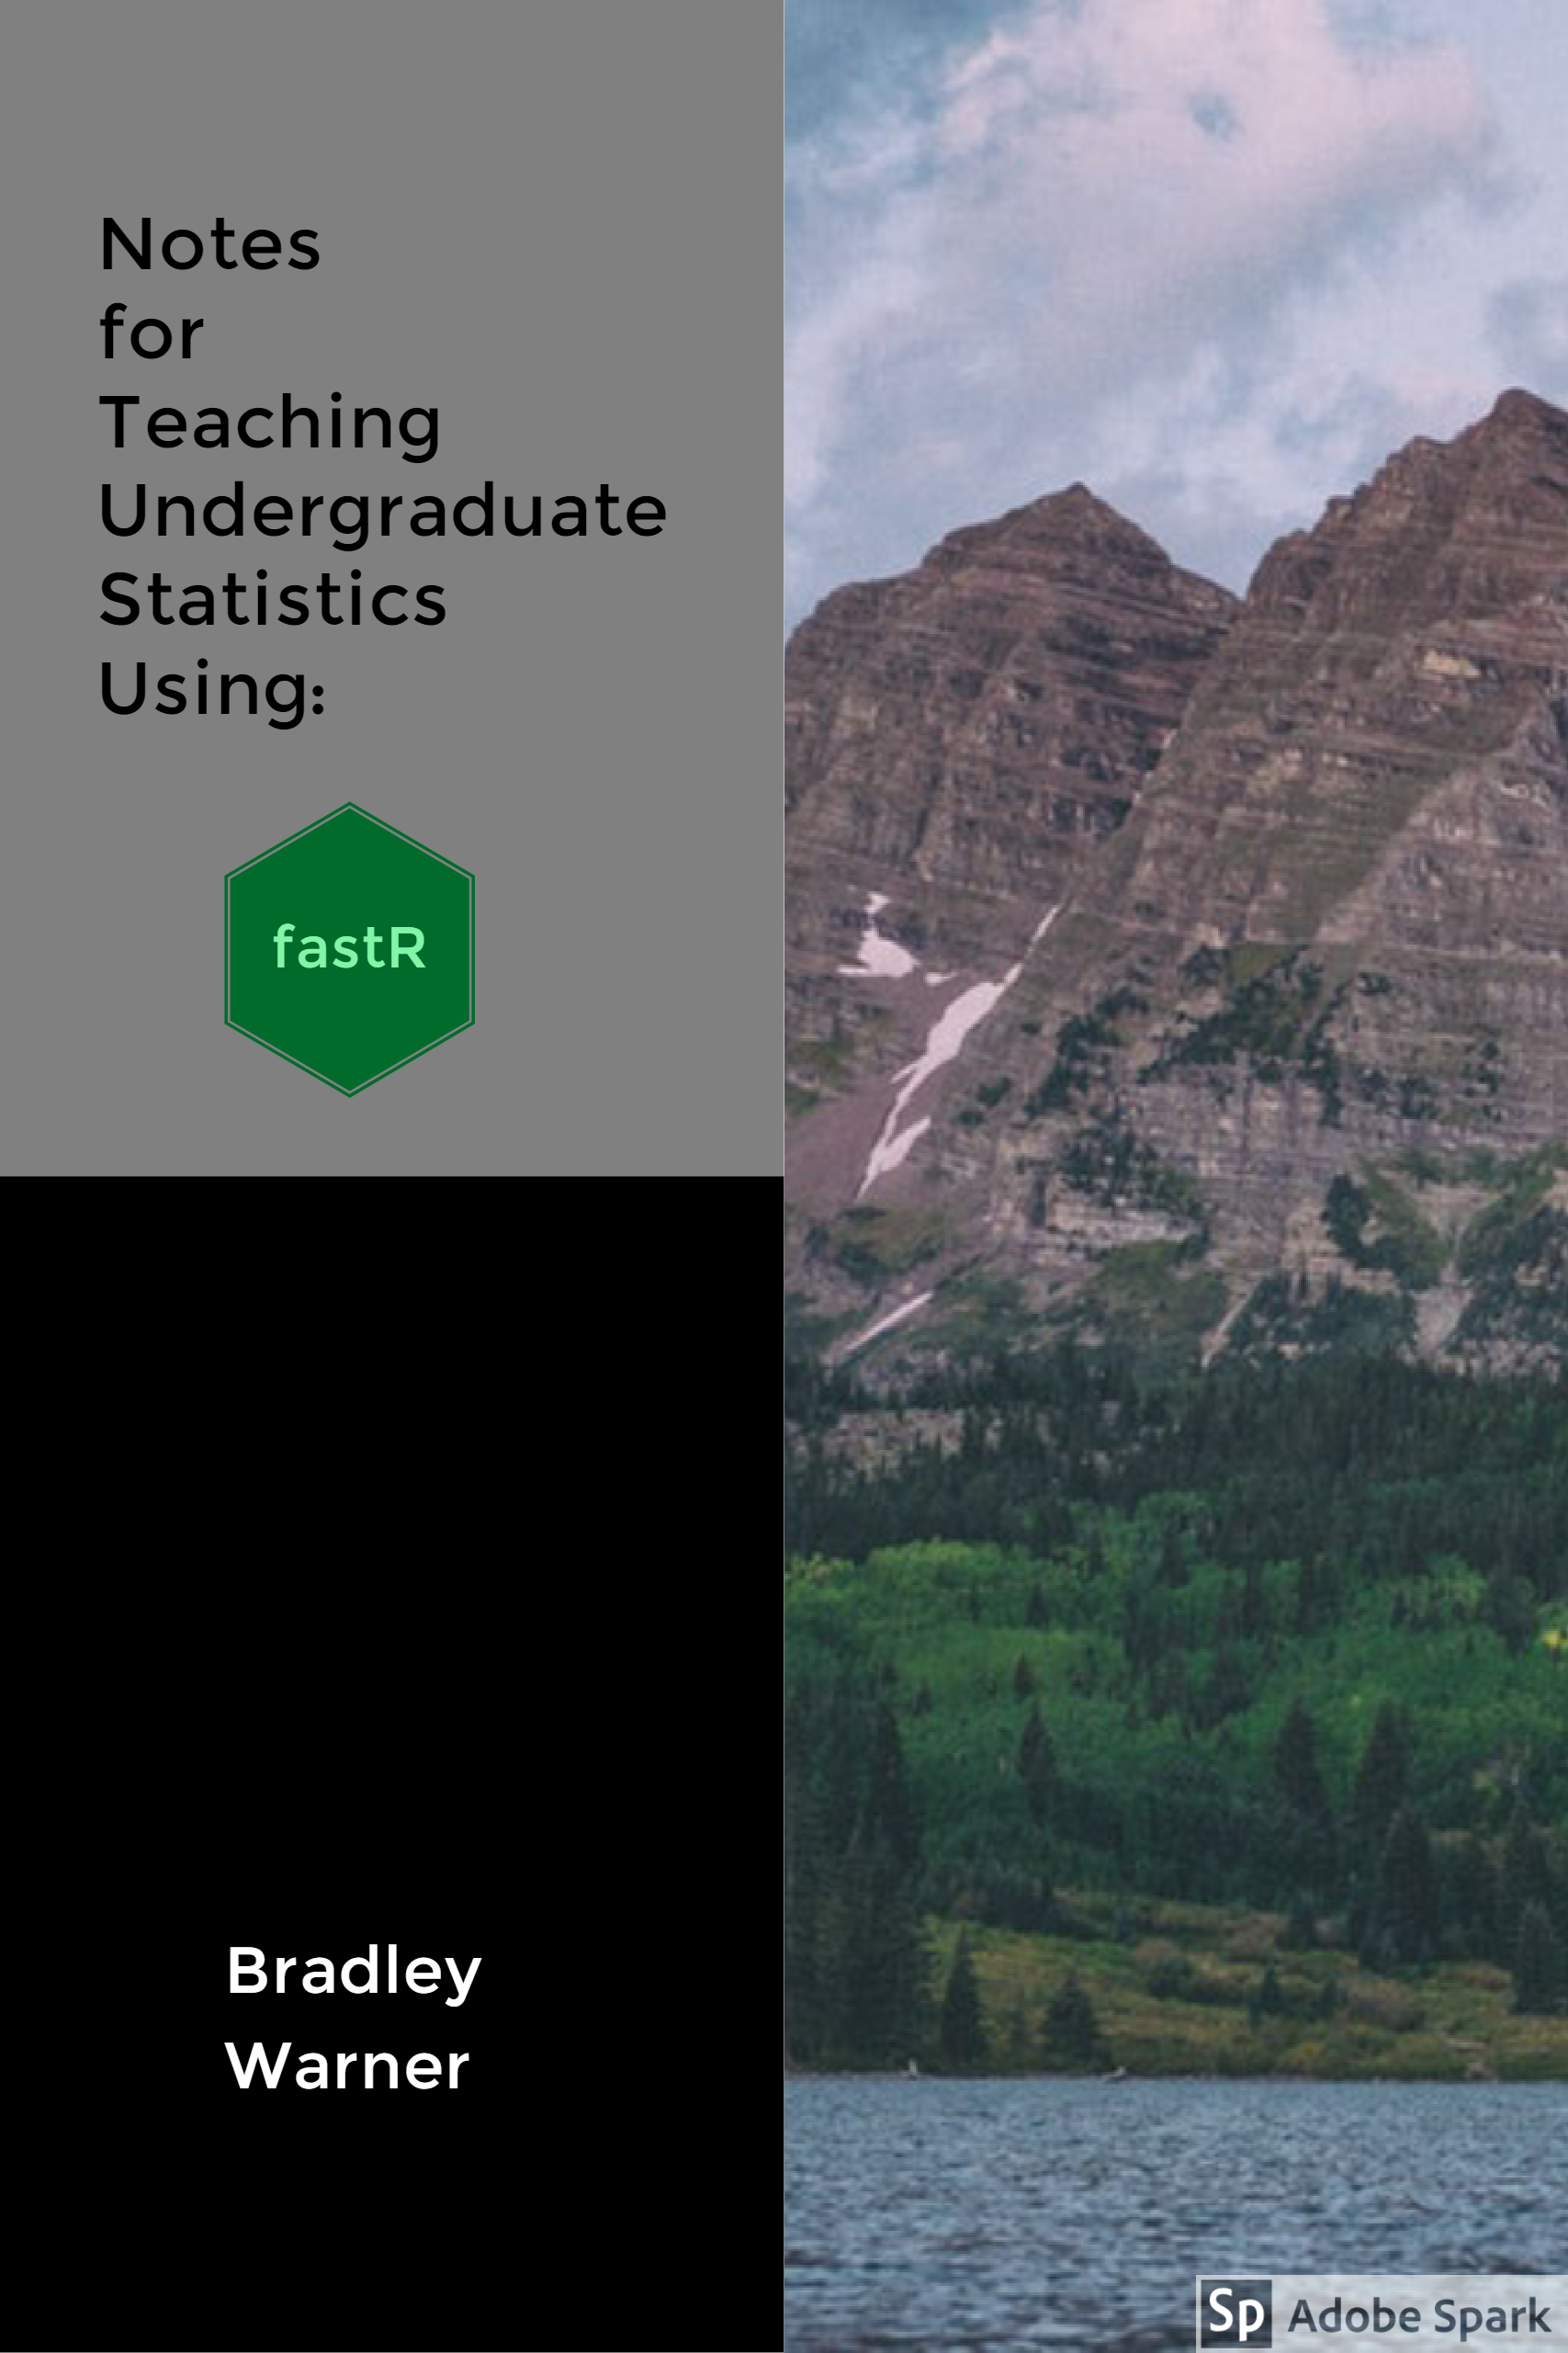
\includegraphics{./images/Cover3.jpg}
\caption{}
\end{figure}

This book is based on the notes I distribute to my students as part of a
one semester course on probability and statistics. I have used these
notes for 3 semesters and so they have seen multiple revisions. This
notes are based on using the first addition of Prium's book Foundations
and Applications of Statistics: An Introduction Using R
\citeyearpar{pruim2011foundations}. I have selected this book because
its cost is reasonable and it does a great job balancing mathematical
rigor with computational skills. I also like the way that R is woven
within the text to include the examples and problems.

\section{Who is this book for?}\label{who-is-this-book-for}

I designed these notes for the instructor who wants to adopt a course
that combines elements of a traditional mathematical statistics course
with more computational and programming emphasis. My subsequent course
is a machine learning course and this course has provided my students
with a solid foundation to approach that next course. I think these
notes will aid any instructor in getting a course with Prium's book up
and running in a short amount of time.

\section{Book Structure and How to Use
It}\label{book-structure-and-how-to-use-it}

In Appendix \ref{AppA}, I have provided my syllabus as an example of how
to use the notes. This syllabus is based on 40 lessons each of 53
minutes long. Obviously this will have to altered based on the length of
course you want to run.

I aligned these notes with the chapters in Prium's textbook. Within each
chapter there are subsections for each lesson. These match the lessons
in the syllabus in Appendix \ref{AppA}.

Every lesson starts with administrative tasks to cover topics such as
upcoming exams, points from previous class that need clarification, and
homework questions. For example, in one lesson I reviewed an RMarkdown
cheat sheet, answered one homework questions, and answered a question on
running swirl. In the notes I have excluded the admin section but be
aware that I have one for each lesson.

I have shortened chapter 5 to allow a brief introduction to linear
regression in chapter 6. The speed of the course is fast and I have had
to make some difficult decisions about what to include and exclude.

I typically include 4 exams in addition to a final. I leave the lesson
before the exam as a review and catch-up day. Thus the 4 exams and 4
review lessons take 8 lessons. The course is fast so I don't mind
putting these extra lessons into the design.

I also include a project I have used in Appendix \ref{AppB}.

\section{Prerequisites}\label{prerequisites}

To take my course, students are expected to have completed calculus up
through and including multivariate calculus. I don't assume they have
any programming experience and thus I have used the swirl package to
help them get started in R. I have the students load and run R locally
on their personal computers and we also use Rstudio as the IDE for our
work.

These notes make use of the following packages in R \textbf{knitr}
\citep{R-knitr}, \textbf{rmarkdown} \citep{R-rmarkdown}, \textbf{fastR}
\citep{R-fastR}, \textbf{Hmisc} \citep{R-Hmisc}, \textbf{lattice}
\citep{R-lattice}, \textbf{vcd} \citep{R-vcd}, \textbf{ggplot2}
\citep{R-ggplot2}, \textbf{MASS} \citep{R-MASS}, \textbf{TeachingDemos}
\citep{R-TeachingDemos}, \textbf{Stat2Data} \citep{R-Stat2Data},
\textbf{car} \citep{R-car}, \textbf{DT} \citep{R-DT}.

\section{Acknowledgements}\label{acknowledgements}

I have been lucky to work with many faculty on this project but would
like to thank Stephanie Bruce and Ken Horton for the willingness to use
and experiment with these notes and for the sound feedback they have
provided.

This book was written using the excellent \textbf{bookdown} package
\citep{R-bookdown}.

\begin{figure}
\centering

\includegraphics{./images/by-nc-sa.png}
\caption{}
\end{figure}

This book is licensed under the
\href{http://creativecommons.org/licenses/by-nc-sa/4.0/}{Creative
Commons Attribution-NonCommercial-ShareAlike 4.0 International License}.

\chapter{Summarizing Data}\label{Chpt1}

The first chapter is completed in three lessons. The first lesson is an
introduction to the course. We make sure that R is installed correctly.
We cover the syllabus and expectations for the course. The next two
lessons break chapter one into two parts, univariate and multivariate
data. What follows are the lesson plans.

\hypertarget{L1}{\section{Admin and Course Introduction}\label{L1}}

\subsection{Objectives}\label{objectives}

\begin{enumerate}
\def\labelenumi{\arabic{enumi}.}
\tightlist
\item
  Introduce the course\\
\item
  Understand classroom expectations\\
\item
  Use R for some basic computations
\end{enumerate}

Material discussed in class:

Why stats and probability?

Math 377 course and purpose

Look at syllabus and due dates

\subsection{In Class Work}\label{in-class-work}

Load and use swirl

Demo R

Load a library and explain installing versus loading:

\begin{Shaded}
\begin{Highlighting}[]
\KeywordTok{library}\NormalTok{(fastR)}
\end{Highlighting}
\end{Shaded}

Look at the structure of a dataframe.

\begin{Shaded}
\begin{Highlighting}[]
\KeywordTok{str}\NormalTok{(students)}
\end{Highlighting}
\end{Shaded}

\begin{verbatim}
## 'data.frame':    1000 obs. of  6 variables:
##  $ ACT    : int  30 20 23 30 21 NA 23 25 30 21 ...
##  $ SAT    : int  NA NA 1060 1420 1010 730 NA NA NA NA ...
##  $ Grad   : logi  TRUE TRUE TRUE TRUE TRUE TRUE ...
##  $ GradGPA: num  3.61 2.99 3.58 3.51 2.7 ...
##  $ HSGPA  : num  3.74 2.97 3.51 3.99 3.25 ...
##  $ Cohort : int  2002 2004 2002 2005 2005 2001 2003 2005 2003 2003 ...
\end{verbatim}

Create a simple plot and comments.

\begin{Shaded}
\begin{Highlighting}[]
\KeywordTok{bwplot}\NormalTok{(Grad}\OperatorTok{~}\NormalTok{HSGPA,students)}
\end{Highlighting}
\end{Shaded}

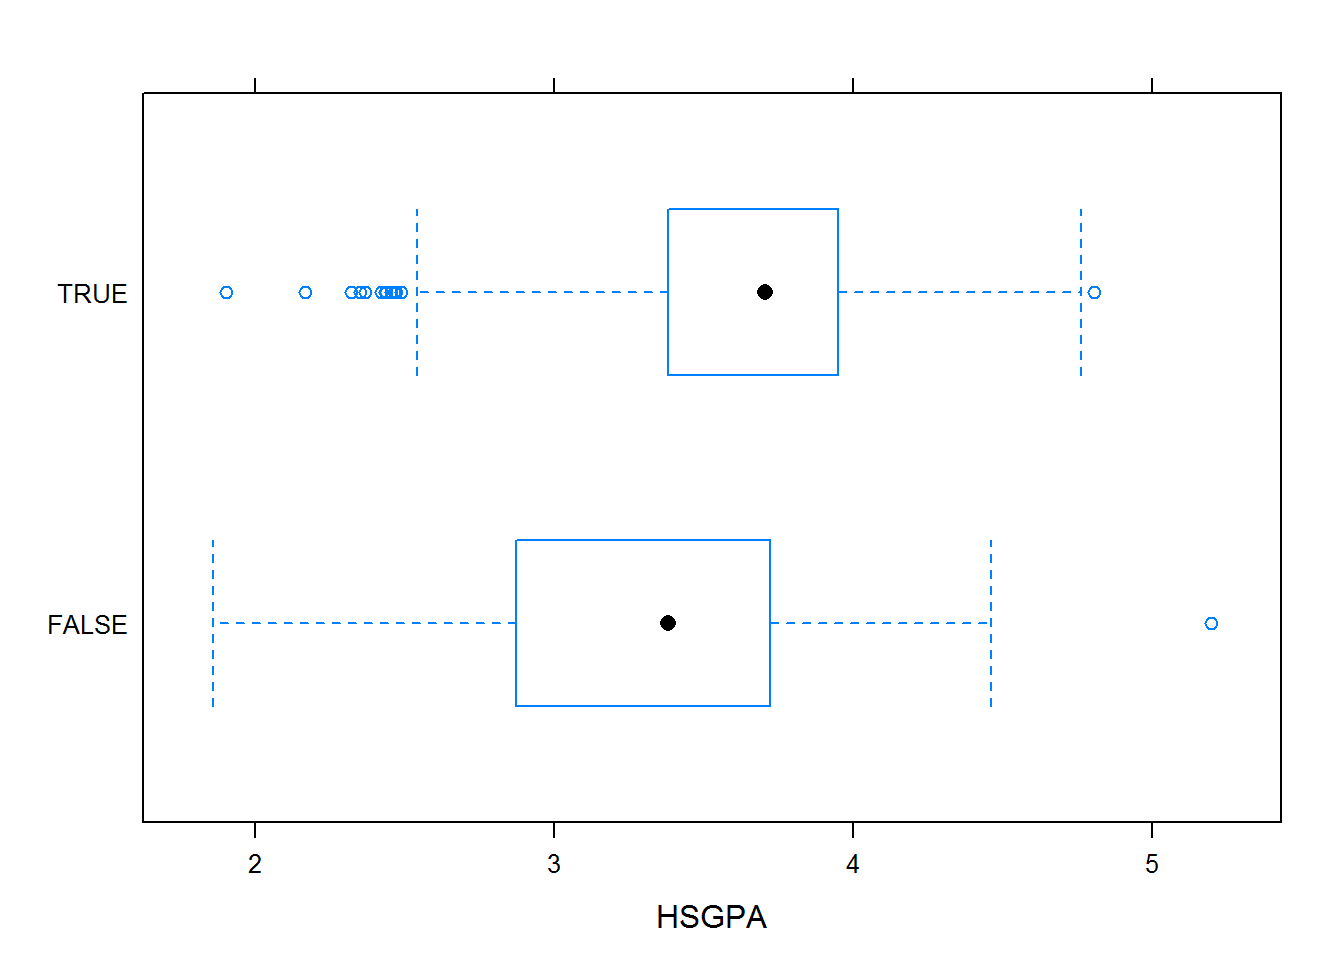
\includegraphics{fastR-Notes_files/figure-latex/unnamed-chunk-5-1.pdf}

\begin{Shaded}
\begin{Highlighting}[]
\CommentTok{# This is a great plot}
\end{Highlighting}
\end{Shaded}

\hypertarget{Les2}{\section{Summarizing Univariate Data}\label{Les2}}

\subsection{Objectives}\label{objectives-1}

\begin{enumerate}
\def\labelenumi{\arabic{enumi}.}
\tightlist
\item
  Create univariate summaries, both numerical and graphical
\item
  Understand and use data structures (e.g.~str, head, \$)
\item
  Learn definitions of new terms such as mean, median, standard
  deviation, and p-quantile.
\end{enumerate}

\subsection{Intro Material}\label{intro-material}

This class is based on empirical deductive reasoning. We have a question
or conjecture and then we collect data and see if it supports or refutes
the conjecture. Often we have only a sample from a population and thus
must you probability to help in the decision.

With the development of powerful computers, we are now also able to
perform empirical inductive reasoning. This is what occurs in the areas
of data mining and machine learning. Math 378 will emphasize these
ideas.

Data is a the heart of both methods.

\subsection{Data Collection}\label{data-collection}

We don't really have a hypothesis at this point just an observation that
this class of Math 377 has some tall people in it. Let's collect the
data and summarize.

It is often easier to enter data in an CSV, comma separated values, in
Excel. We will then read the data into a data frame in R. This is done
using the import tab in RStudio.

Open a new RMarkdown file to store our work.

Now that we have the data and before we start, let's practice some of
the ideas in Sections 1.1 and 1.2 of the book.

\subsection{Background}\label{background}

Load libraries.

\begin{Shaded}
\begin{Highlighting}[]
\KeywordTok{library}\NormalTok{(}\StringTok{'fastR'}\NormalTok{)}
\KeywordTok{library}\NormalTok{(Hmisc)}
\KeywordTok{library}\NormalTok{(lattice)}
\end{Highlighting}
\end{Shaded}

Look at available data sets. Use the command.

\begin{verbatim}
data()
\end{verbatim}

Let's use the data set students in the fastR package. Before we start,
let's get a feel for the data.

The \texttt{str} function gives the structure of the data

\begin{Shaded}
\begin{Highlighting}[]
\KeywordTok{str}\NormalTok{(students)}
\end{Highlighting}
\end{Shaded}

\begin{verbatim}
## 'data.frame':    1000 obs. of  6 variables:
##  $ ACT    : int  30 20 23 30 21 NA 23 25 30 21 ...
##  $ SAT    : int  NA NA 1060 1420 1010 730 NA NA NA NA ...
##  $ Grad   : logi  TRUE TRUE TRUE TRUE TRUE TRUE ...
##  $ GradGPA: num  3.61 2.99 3.58 3.51 2.7 ...
##  $ HSGPA  : num  3.74 2.97 3.51 3.99 3.25 ...
##  $ Cohort : int  2002 2004 2002 2005 2005 2001 2003 2005 2003 2003 ...
\end{verbatim}

To look at the first few rows

\begin{Shaded}
\begin{Highlighting}[]
\KeywordTok{head}\NormalTok{(students)}
\end{Highlighting}
\end{Shaded}

\begin{verbatim}
##   ACT  SAT Grad GradGPA HSGPA Cohort
## 1  30   NA TRUE   3.613 3.743   2002
## 2  20   NA TRUE   2.993 2.968   2004
## 3  23 1060 TRUE   3.582 3.507   2002
## 4  30 1420 TRUE   3.513 3.990   2005
## 5  21 1010 TRUE   2.703 3.253   2005
## 6  NA  730 TRUE   3.360 2.621   2001
\end{verbatim}

If you want a nice output when you knit into an html or pdf file

\begin{Shaded}
\begin{Highlighting}[]
\NormalTok{knitr}\OperatorTok{::}\KeywordTok{kable}\NormalTok{(}
\KeywordTok{head}\NormalTok{(students)}
\NormalTok{)}
\end{Highlighting}
\end{Shaded}

\begin{tabular}{r|r|l|r|r|r}
\hline
ACT & SAT & Grad & GradGPA & HSGPA & Cohort\\
\hline
30 & NA & TRUE & 3.613 & 3.743 & 2002\\
\hline
20 & NA & TRUE & 2.993 & 2.968 & 2004\\
\hline
23 & 1060 & TRUE & 3.582 & 3.507 & 2002\\
\hline
30 & 1420 & TRUE & 3.513 & 3.990 & 2005\\
\hline
21 & 1010 & TRUE & 2.703 & 3.253 & 2005\\
\hline
NA & 730 & TRUE & 3.360 & 2.621 & 2001\\
\hline
\end{tabular}

\begin{Shaded}
\begin{Highlighting}[]
\KeywordTok{summary}\NormalTok{(students)}
\end{Highlighting}
\end{Shaded}

\begin{verbatim}
##       ACT             SAT          Grad            GradGPA     
##  Min.   :14.00   Min.   : 730   Mode :logical   Min.   :2.075  
##  1st Qu.:23.00   1st Qu.:1080   FALSE:268       1st Qu.:3.033  
##  Median :26.00   Median :1180   TRUE :732       Median :3.389  
##  Mean   :25.94   Mean   :1199                   Mean   :3.322  
##  3rd Qu.:29.00   3rd Qu.:1310                   3rd Qu.:3.657  
##  Max.   :36.00   Max.   :1590                   Max.   :4.000  
##  NA's   :169     NA's   :636                    NA's   :268    
##      HSGPA           Cohort    
##  Min.   :1.857   Min.   :2001  
##  1st Qu.:3.252   1st Qu.:2002  
##  Median :3.635   Median :2003  
##  Mean   :3.546   Mean   :2003  
##  3rd Qu.:3.912   3rd Qu.:2004  
##  Max.   :5.197   Max.   :2005  
##  NA's   :16
\end{verbatim}

You can also use the help menu to find out more about the data,
\texttt{?students}

Some basic summaries of the data. Since \texttt{Grad} is discrete we
summarize with a table.

\begin{Shaded}
\begin{Highlighting}[]
\KeywordTok{table}\NormalTok{(students}\OperatorTok{$}\NormalTok{Grad)}
\end{Highlighting}
\end{Shaded}

\begin{verbatim}
## 
## FALSE  TRUE 
##   268   732
\end{verbatim}

The variable \texttt{HSGPA} is more like a continuous variable.

\begin{Shaded}
\begin{Highlighting}[]
\KeywordTok{mean}\NormalTok{(students}\OperatorTok{$}\NormalTok{HSGPA,}\DataTypeTok{na.rm=}\OtherTok{TRUE}\NormalTok{)}
\end{Highlighting}
\end{Shaded}

\begin{verbatim}
## [1] 3.545669
\end{verbatim}

\begin{Shaded}
\begin{Highlighting}[]
\KeywordTok{median}\NormalTok{(students}\OperatorTok{$}\NormalTok{HSGPA,}\DataTypeTok{na.rm=}\OtherTok{TRUE}\NormalTok{)}
\end{Highlighting}
\end{Shaded}

\begin{verbatim}
## [1] 3.6345
\end{verbatim}

\begin{Shaded}
\begin{Highlighting}[]
\KeywordTok{quantile}\NormalTok{(students}\OperatorTok{$}\NormalTok{HSGPA,}\DataTypeTok{na.rm =} \OtherTok{TRUE}\NormalTok{)}
\end{Highlighting}
\end{Shaded}

\begin{verbatim}
##      0%     25%     50%     75%    100% 
## 1.85700 3.25250 3.63450 3.91225 5.19700
\end{verbatim}

The calculation of quantiles can be confusing, but the book does a nice
job explaining how it is done. We can also get help on the function
using \texttt{?quantile}.

Notice that if we did remove missing values, we would get an
\texttt{NA}.

\begin{Shaded}
\begin{Highlighting}[]
\KeywordTok{mean}\NormalTok{(students}\OperatorTok{$}\NormalTok{HSGPA)}
\end{Highlighting}
\end{Shaded}

\begin{verbatim}
## [1] NA
\end{verbatim}

For dispersion, we can summarize with variance and standard deviation.

\begin{Shaded}
\begin{Highlighting}[]
\KeywordTok{sd}\NormalTok{(}\OperatorTok{~}\NormalTok{GradGPA,}\DataTypeTok{data=}\NormalTok{students,}\DataTypeTok{na.rm=}\NormalTok{T)}
\end{Highlighting}
\end{Shaded}

\begin{verbatim}
## [1] 0.4220109
\end{verbatim}

\begin{Shaded}
\begin{Highlighting}[]
\KeywordTok{sd}\NormalTok{(students}\OperatorTok{$}\NormalTok{GradGPA,}\DataTypeTok{na.rm=}\NormalTok{T)}
\end{Highlighting}
\end{Shaded}

\begin{verbatim}
## [1] 0.4220109
\end{verbatim}

\begin{Shaded}
\begin{Highlighting}[]
\KeywordTok{var}\NormalTok{(students}\OperatorTok{$}\NormalTok{GradGPA,}\DataTypeTok{na.rm=}\NormalTok{T)}
\end{Highlighting}
\end{Shaded}

\begin{verbatim}
## [1] 0.1780932
\end{verbatim}

A useful function in the mosaic package is favstats.

\begin{Shaded}
\begin{Highlighting}[]
\KeywordTok{favstats}\NormalTok{(}\OperatorTok{~}\NormalTok{HSGPA,}\DataTypeTok{data=}\NormalTok{students)}
\end{Highlighting}
\end{Shaded}

\begin{verbatim}
##    min     Q1 median      Q3   max     mean        sd   n missing
##  1.857 3.2525 3.6345 3.91225 5.197 3.545669 0.4793097 984      16
\end{verbatim}

Notice we used the R formula notation discussed in the book.

Breaking it down by year group.

\begin{Shaded}
\begin{Highlighting}[]
\KeywordTok{favstats}\NormalTok{(HSGPA}\OperatorTok{~}\NormalTok{Cohort,}\DataTypeTok{data=}\NormalTok{students)}
\end{Highlighting}
\end{Shaded}

\begin{verbatim}
##   Cohort   min      Q1 median      Q3   max     mean        sd   n missing
## 1   2001 2.167 3.16350 3.6195 3.88575 5.197 3.502119 0.5393179 194       6
## 2   2002 2.320 3.34325 3.6940 3.92825 4.705 3.600908 0.4266389 218       3
## 3   2003 1.857 3.25100 3.6905 3.90925 4.762 3.563235 0.4829192 200       4
## 4   2004 2.160 3.28400 3.6200 3.90600 4.806 3.544259 0.4631015 185       2
## 5   2005 1.900 3.24950 3.5650 3.92600 4.337 3.509059 0.4807082 187       1
\end{verbatim}

\begin{Shaded}
\begin{Highlighting}[]
\KeywordTok{summary}\NormalTok{(HSGPA}\OperatorTok{~}\NormalTok{Grad,}\DataTypeTok{data=}\NormalTok{students,}\DataTypeTok{fun=}\NormalTok{favstats)}
\end{Highlighting}
\end{Shaded}

\begin{verbatim}
## HSGPA     N= 984 , 16 Missing 
## 
## +-------+---+---+-----+------+-------+-------+-----+--------+---------+---+--------+
## |       |   |N  |min  |Q1    |median |Q3     |max  |mean    |sd       |n  |missing |
## +-------+---+---+-----+------+-------+-------+-----+--------+---------+---+--------+
## |Grad   |No |263|1.857|2.8730|3.3800 |3.72250|5.197|3.307817|0.5373946|263|0       |
## |       |Yes|721|1.900|3.3800|3.7040 |3.94900|4.806|3.632430|0.4246933|721|0       |
## +-------+---+---+-----+------+-------+-------+-----+--------+---------+---+--------+
## |Overall|   |984|1.857|3.2525|3.6345 |3.91225|5.197|3.545669|0.4793097|984|0       |
## +-------+---+---+-----+------+-------+-------+-----+--------+---------+---+--------+
\end{verbatim}

Visual summaries. The command \texttt{hist} is in the base package while
\texttt{histogram} is in lattice.

\begin{Shaded}
\begin{Highlighting}[]
\KeywordTok{hist}\NormalTok{(students}\OperatorTok{$}\NormalTok{HSGPA)}
\end{Highlighting}
\end{Shaded}

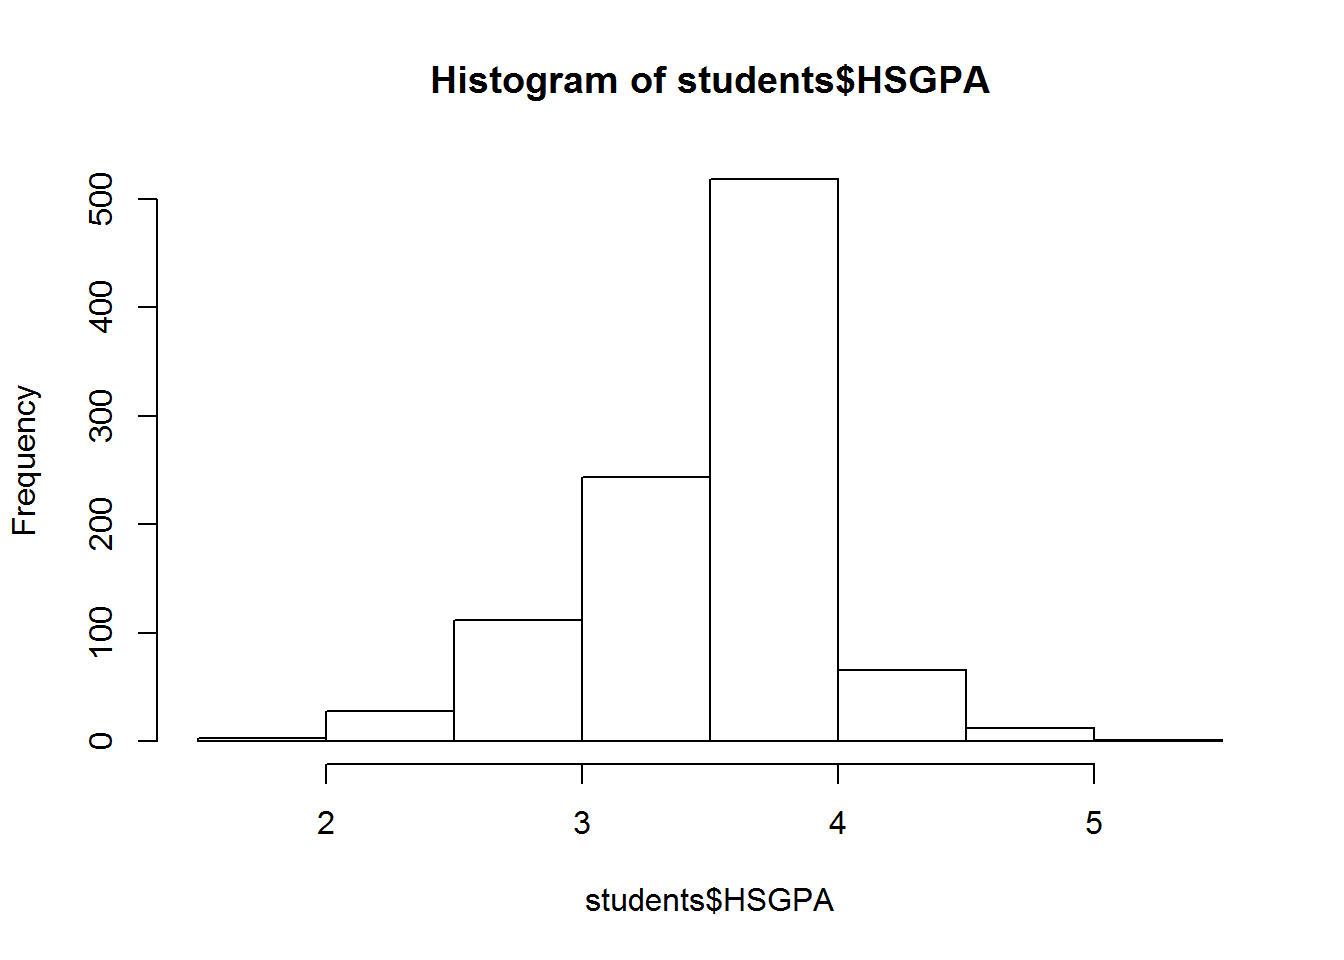
\includegraphics{fastR-Notes_files/figure-latex/unnamed-chunk-18-1.pdf}

With a title.

\begin{Shaded}
\begin{Highlighting}[]
\KeywordTok{hist}\NormalTok{(students}\OperatorTok{$}\NormalTok{HSGPA,}\DataTypeTok{main=}\StringTok{"High School GPA"}\NormalTok{)}
\end{Highlighting}
\end{Shaded}

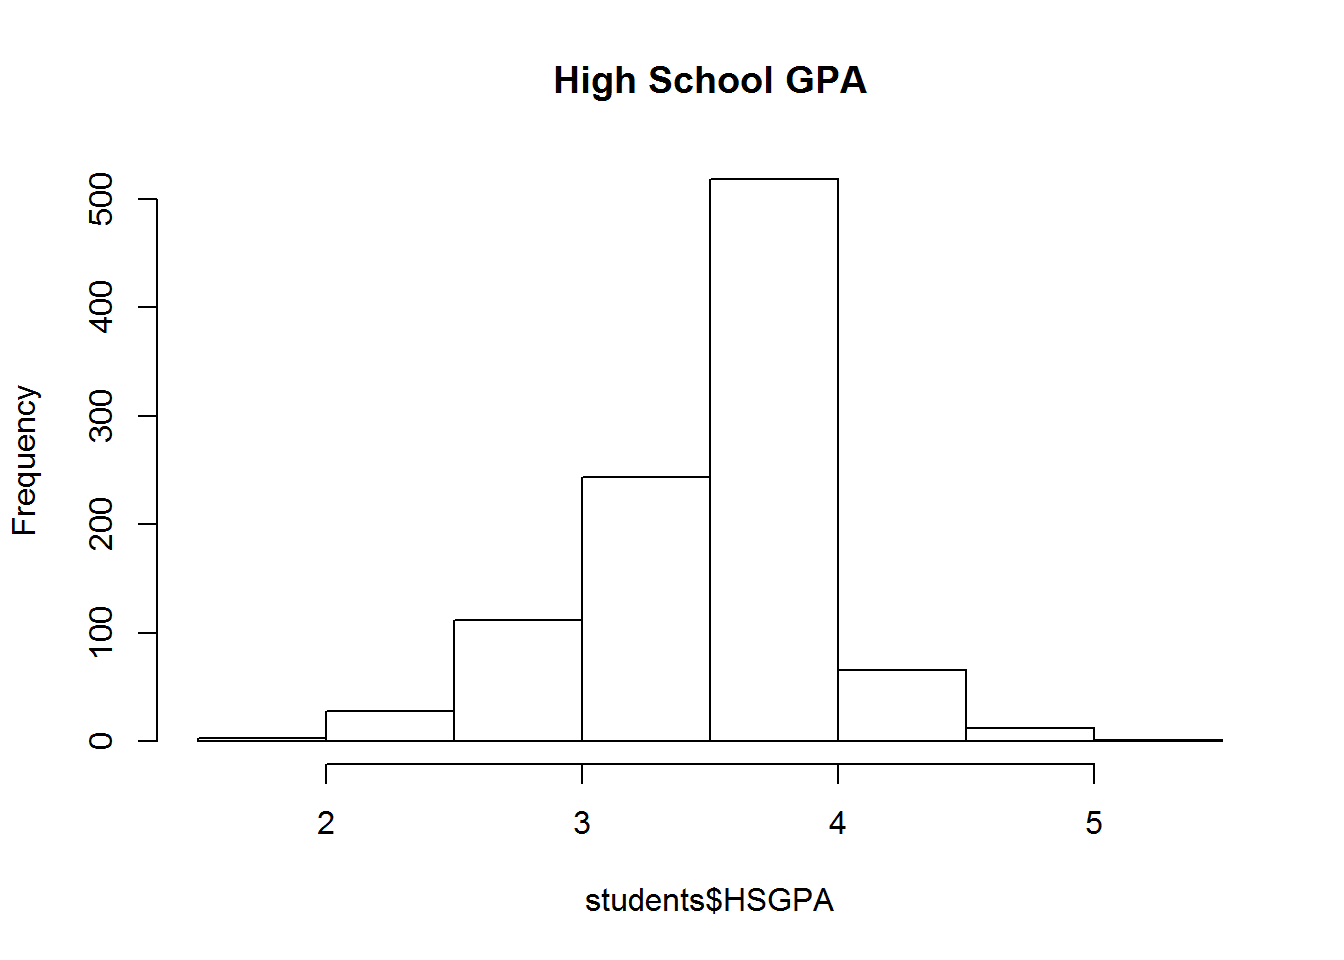
\includegraphics{fastR-Notes_files/figure-latex/unnamed-chunk-19-1.pdf}

The command \texttt{histogram} has more options.

\begin{Shaded}
\begin{Highlighting}[]
\KeywordTok{histogram}\NormalTok{(students}\OperatorTok{$}\NormalTok{HSGPA)}
\end{Highlighting}
\end{Shaded}

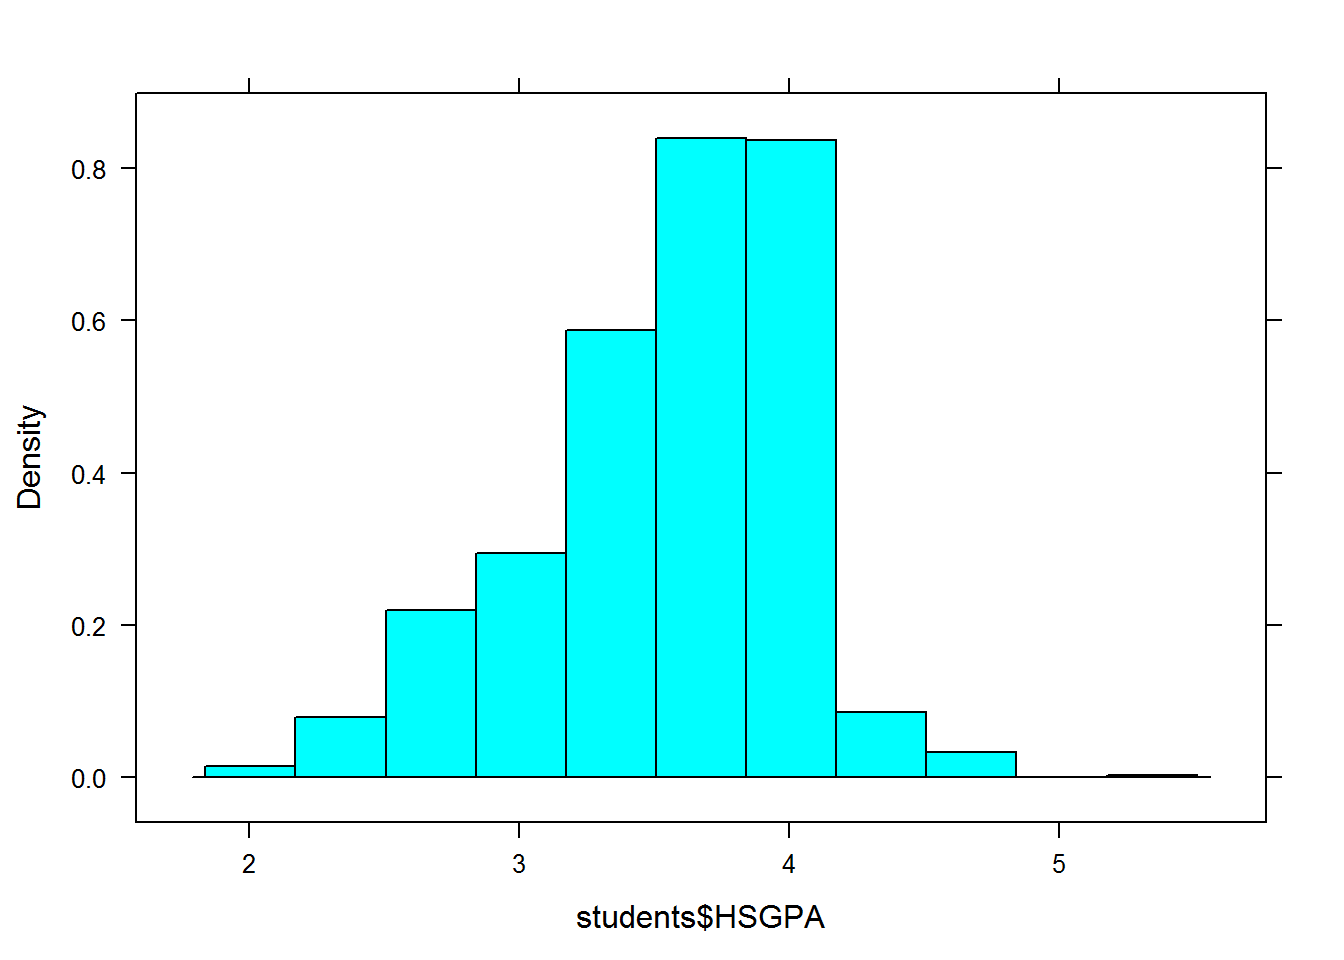
\includegraphics{fastR-Notes_files/figure-latex/unnamed-chunk-20-1.pdf}

\begin{Shaded}
\begin{Highlighting}[]
\KeywordTok{histogram}\NormalTok{(students}\OperatorTok{$}\NormalTok{HSGPA,}\DataTypeTok{type=}\StringTok{"count"}\NormalTok{)}
\end{Highlighting}
\end{Shaded}

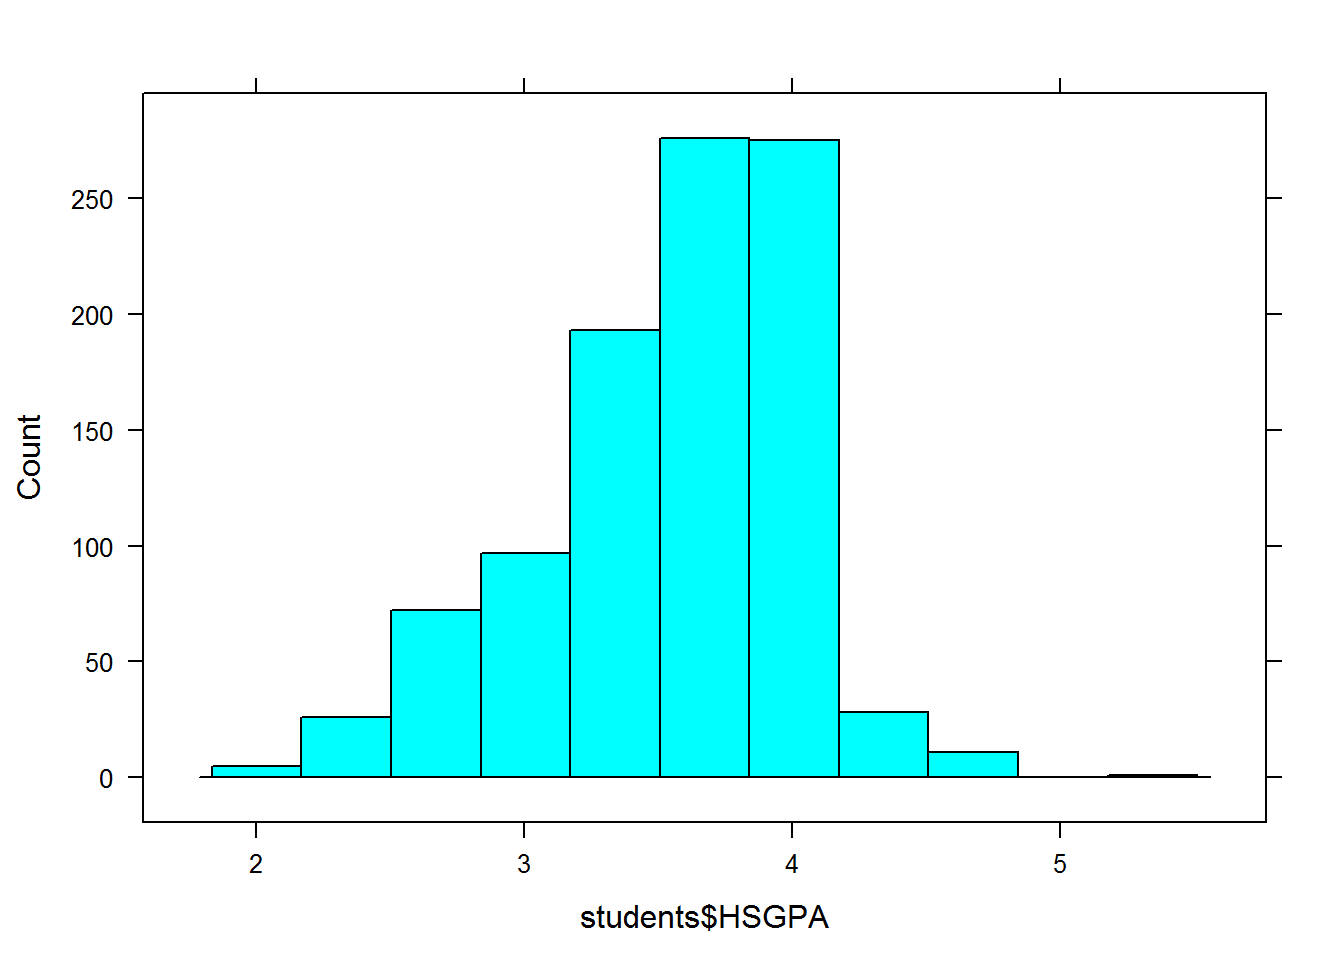
\includegraphics{fastR-Notes_files/figure-latex/unnamed-chunk-21-1.pdf}

A panel display to show histograms next to each other.

\begin{Shaded}
\begin{Highlighting}[]
\KeywordTok{histogram}\NormalTok{(}\OperatorTok{~}\NormalTok{HSGPA}\OperatorTok{|}\KeywordTok{factor}\NormalTok{(Cohort),}\DataTypeTok{data=}\NormalTok{students)}
\end{Highlighting}
\end{Shaded}

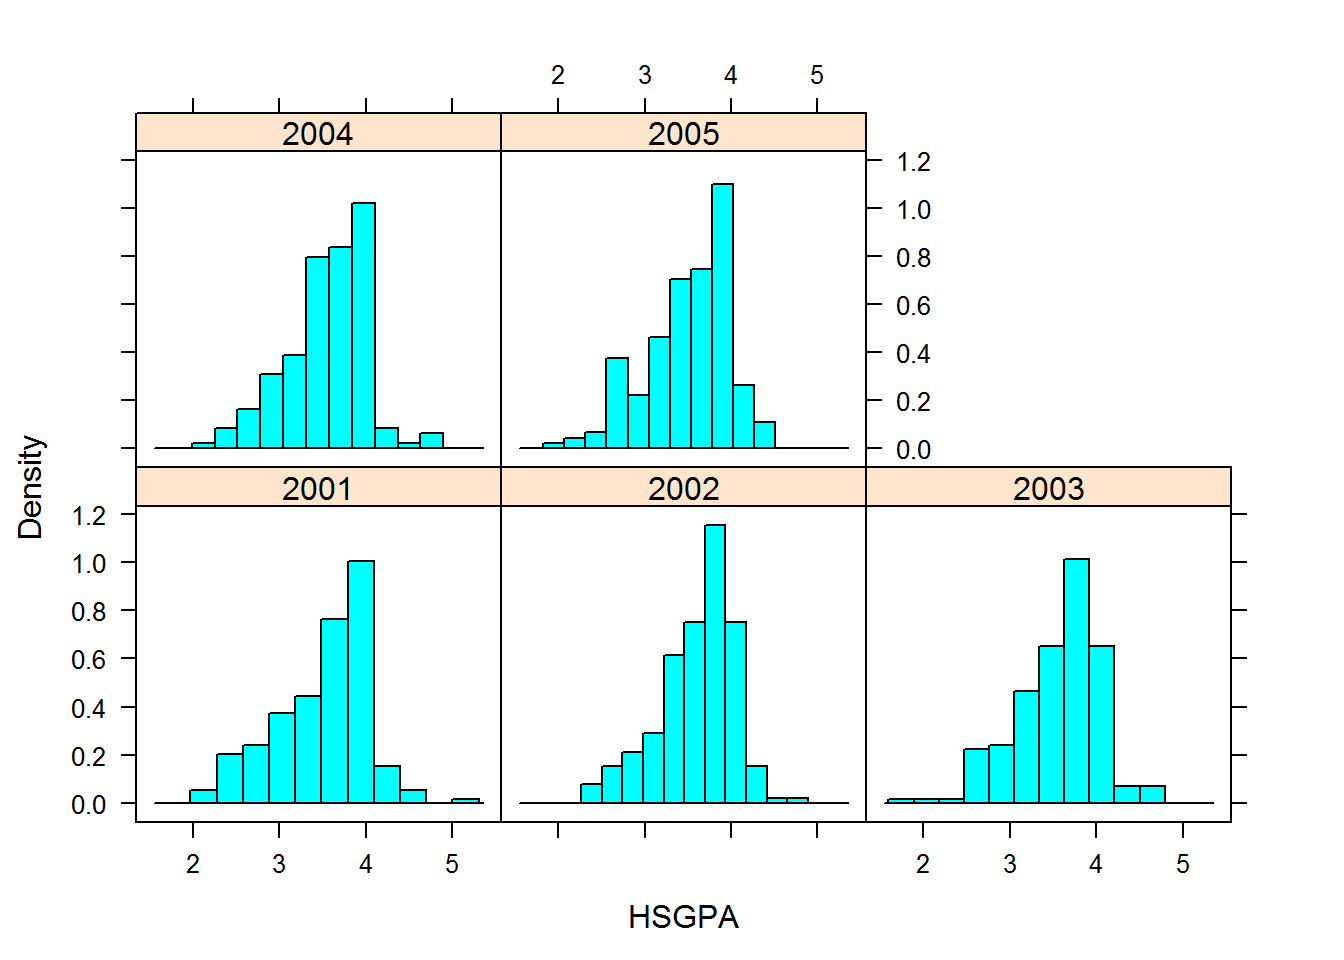
\includegraphics{fastR-Notes_files/figure-latex/unnamed-chunk-22-1.pdf}

Another type of plot is the box and whiskers plot.

From the base package.

\begin{Shaded}
\begin{Highlighting}[]
\KeywordTok{boxplot}\NormalTok{(students}\OperatorTok{$}\NormalTok{HSGPA)}
\end{Highlighting}
\end{Shaded}

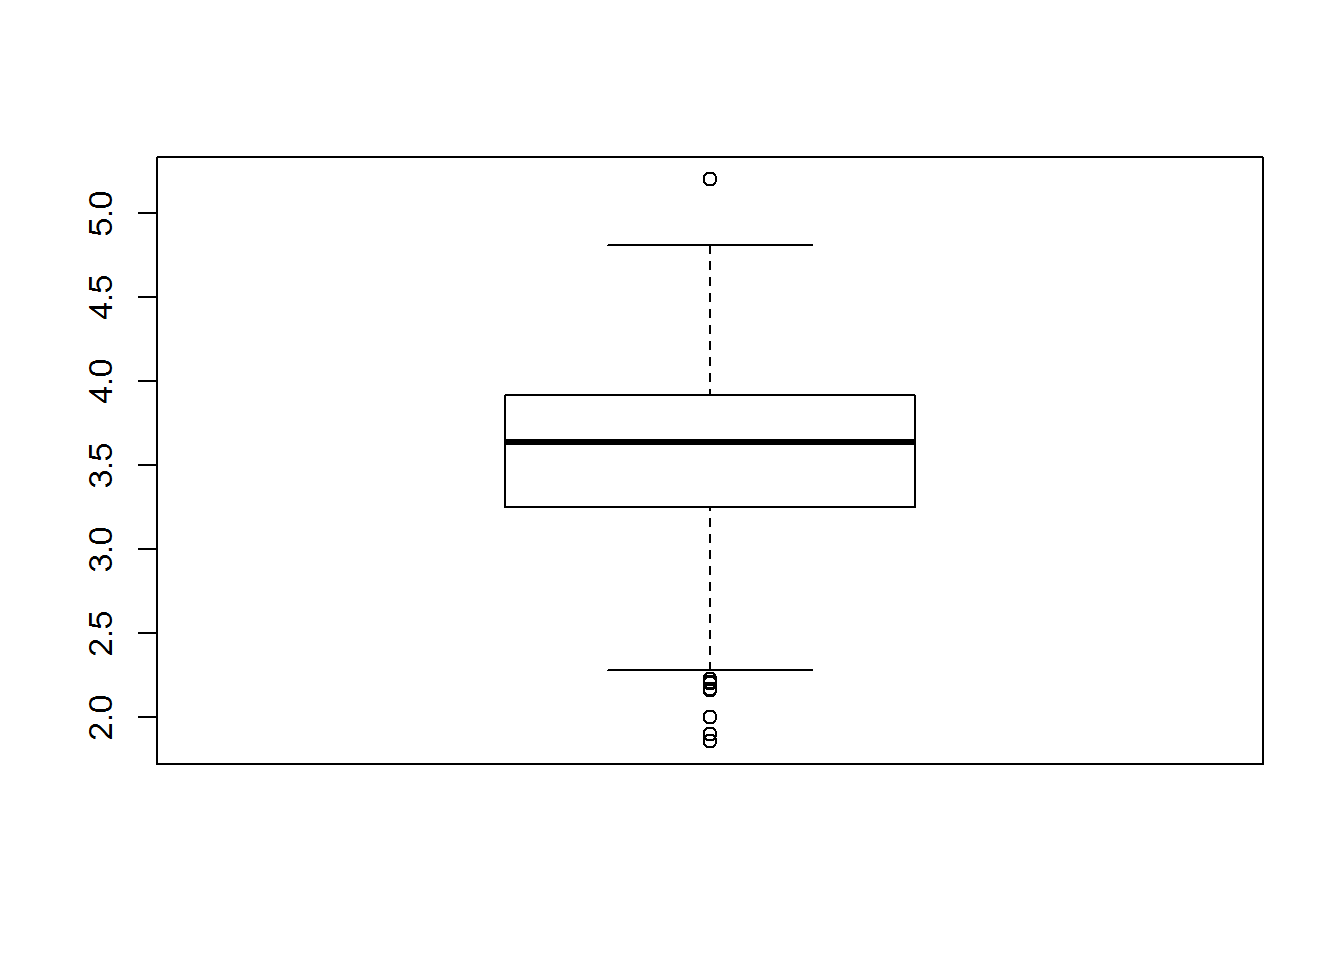
\includegraphics{fastR-Notes_files/figure-latex/unnamed-chunk-23-1.pdf}

And from lattice.

\begin{Shaded}
\begin{Highlighting}[]
\KeywordTok{bwplot}\NormalTok{(}\OperatorTok{~}\NormalTok{HSGPA,students)}
\end{Highlighting}
\end{Shaded}

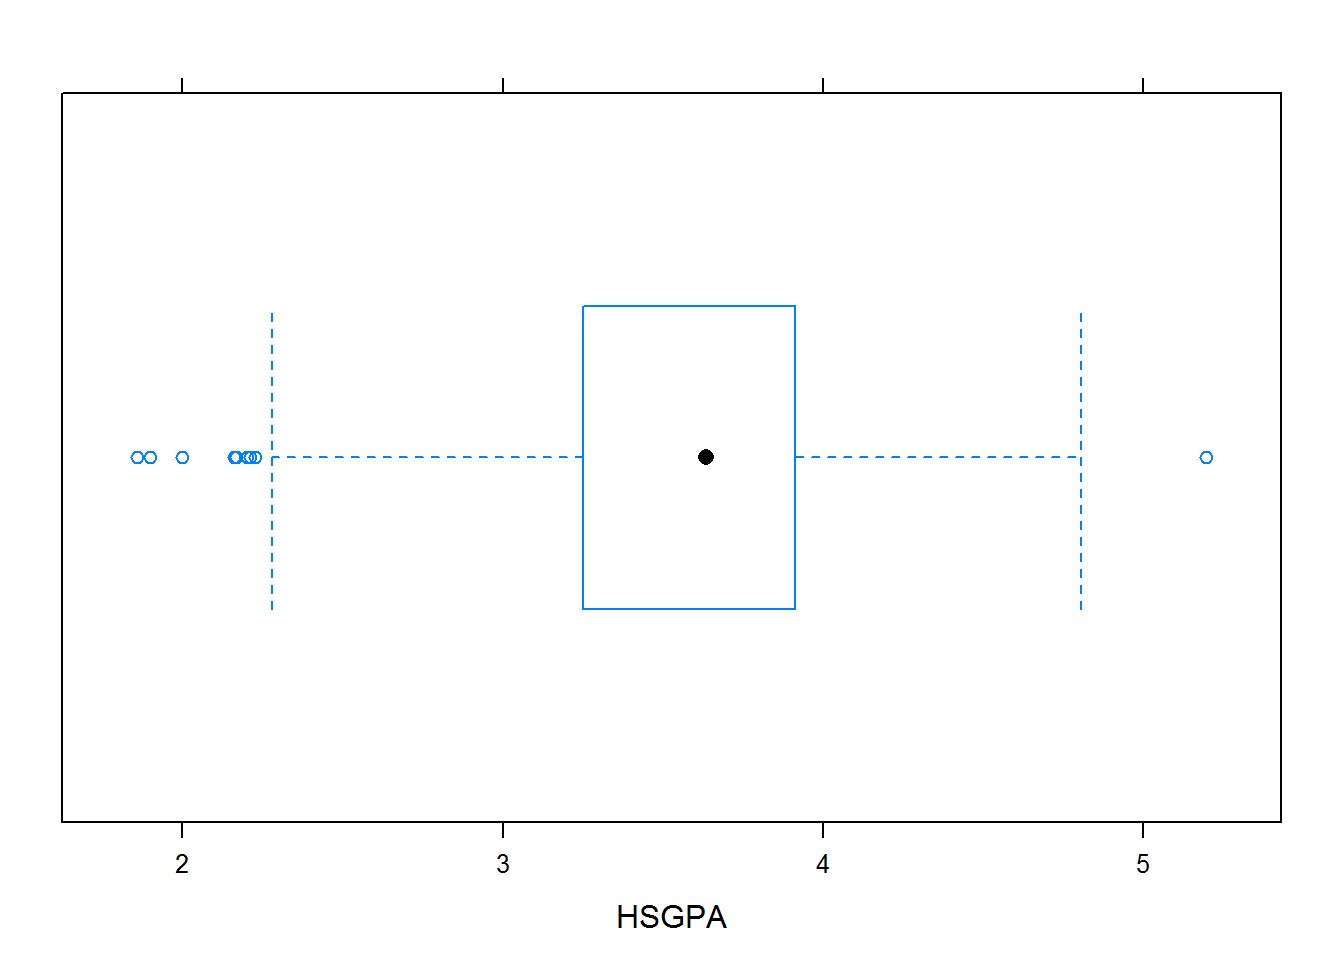
\includegraphics{fastR-Notes_files/figure-latex/unnamed-chunk-24-1.pdf}

\begin{Shaded}
\begin{Highlighting}[]
\KeywordTok{bwplot}\NormalTok{(}\OperatorTok{~}\NormalTok{HSGPA}\OperatorTok{|}\KeywordTok{factor}\NormalTok{(Cohort),students)}
\end{Highlighting}
\end{Shaded}

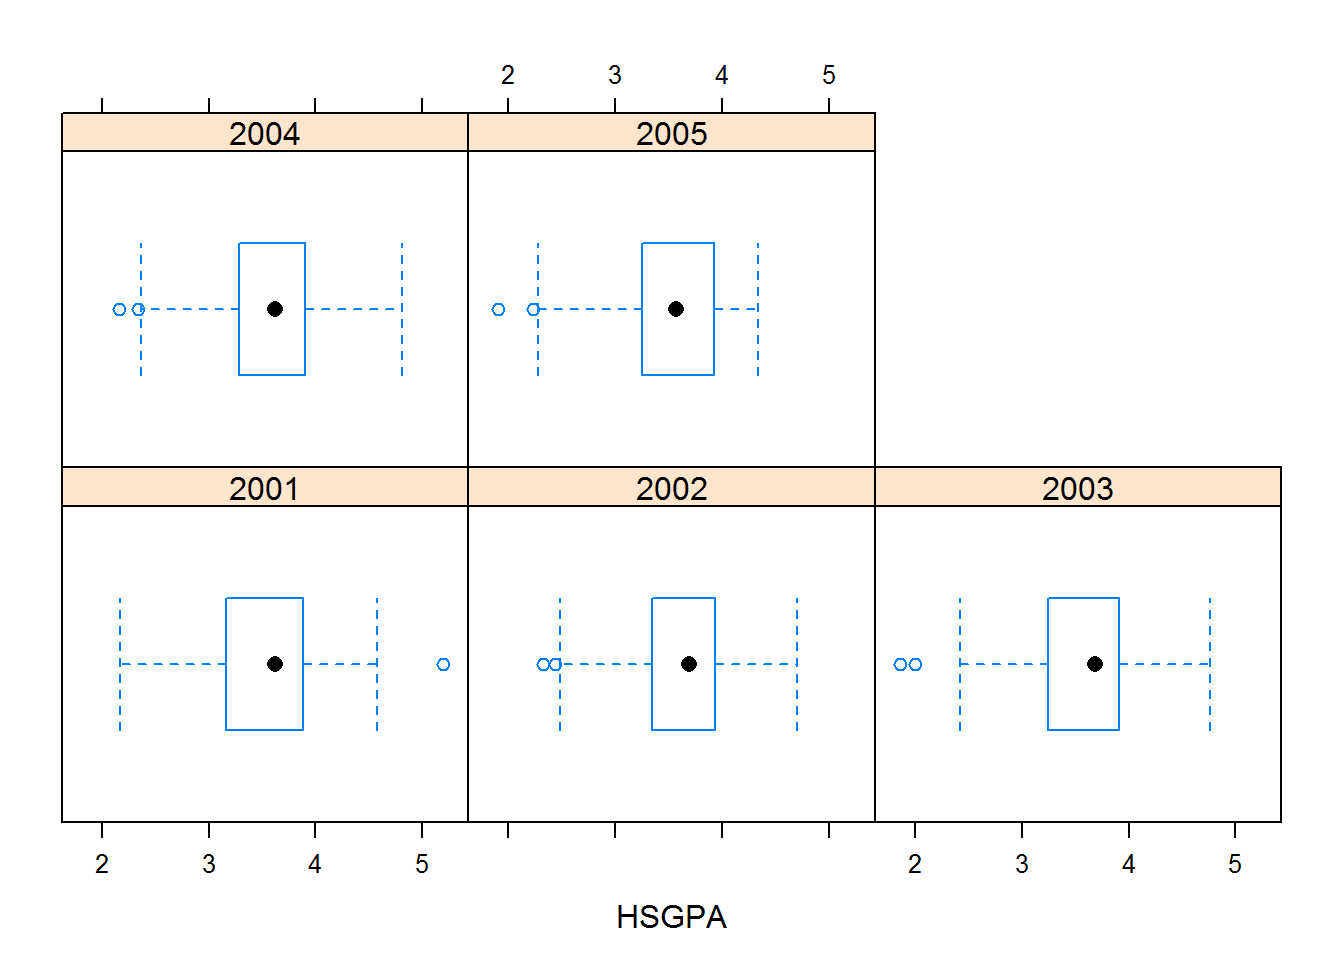
\includegraphics{fastR-Notes_files/figure-latex/unnamed-chunk-25-1.pdf}

\begin{Shaded}
\begin{Highlighting}[]
\KeywordTok{bwplot}\NormalTok{(HSGPA}\OperatorTok{~}\KeywordTok{factor}\NormalTok{(Cohort),students)}
\end{Highlighting}
\end{Shaded}

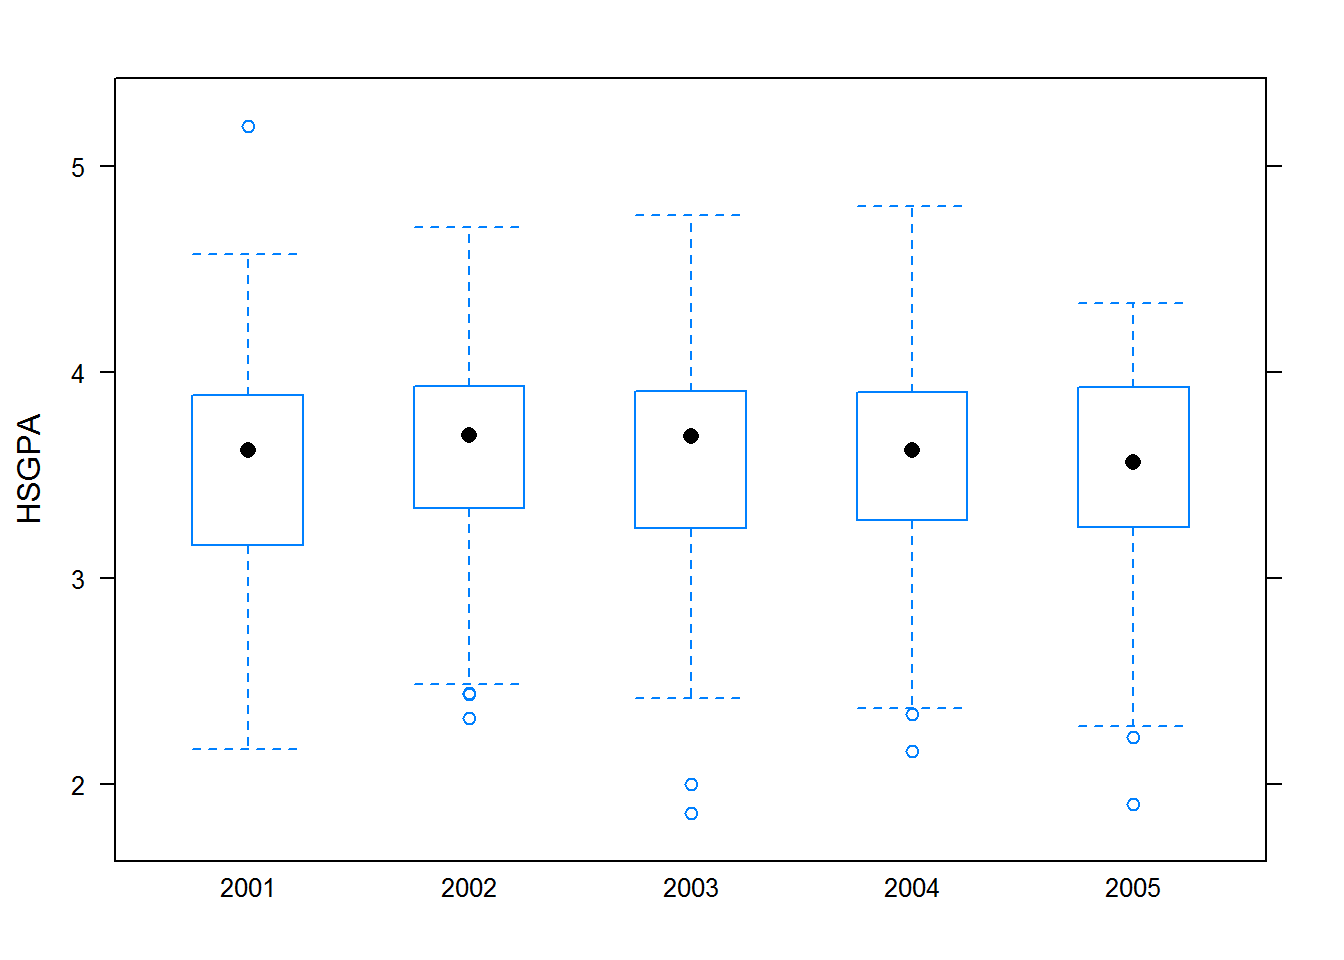
\includegraphics{fastR-Notes_files/figure-latex/unnamed-chunk-26-1.pdf}

Histograms are notoriously sensitive to the parameters used to build
them such as number of bins and location of bins. A better method is to
use a density plot.

\begin{Shaded}
\begin{Highlighting}[]
\KeywordTok{plot}\NormalTok{(}\KeywordTok{density}\NormalTok{(students}\OperatorTok{$}\NormalTok{HSGPA,}\DataTypeTok{na.rm=}\NormalTok{T))}
\end{Highlighting}
\end{Shaded}

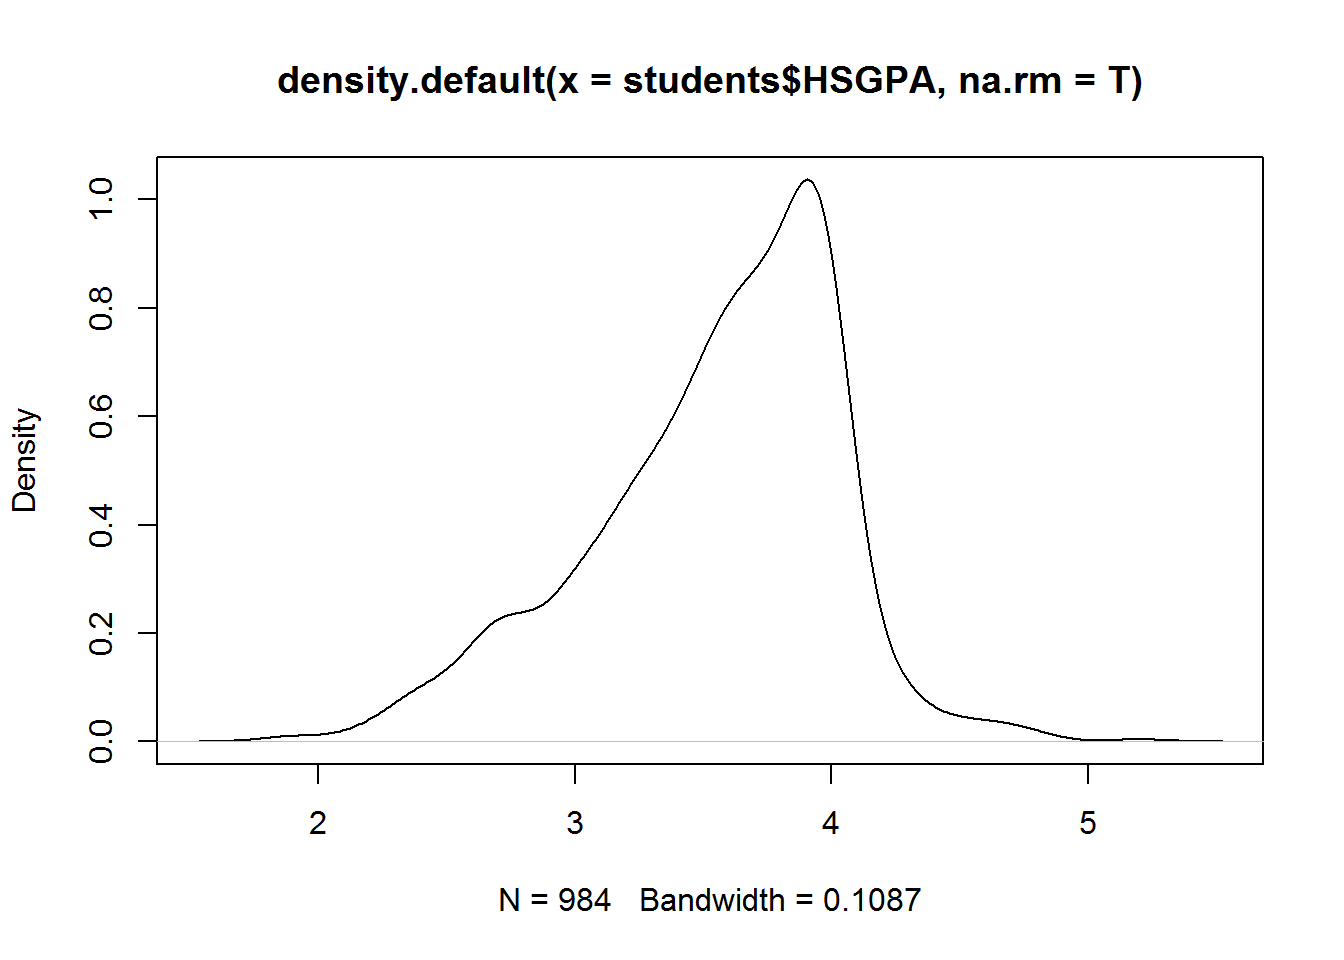
\includegraphics{fastR-Notes_files/figure-latex/unnamed-chunk-27-1.pdf}

And for interest, another variable.

\begin{Shaded}
\begin{Highlighting}[]
\KeywordTok{bwplot}\NormalTok{(GradGPA}\OperatorTok{~}\KeywordTok{factor}\NormalTok{(Cohort),students)}
\end{Highlighting}
\end{Shaded}

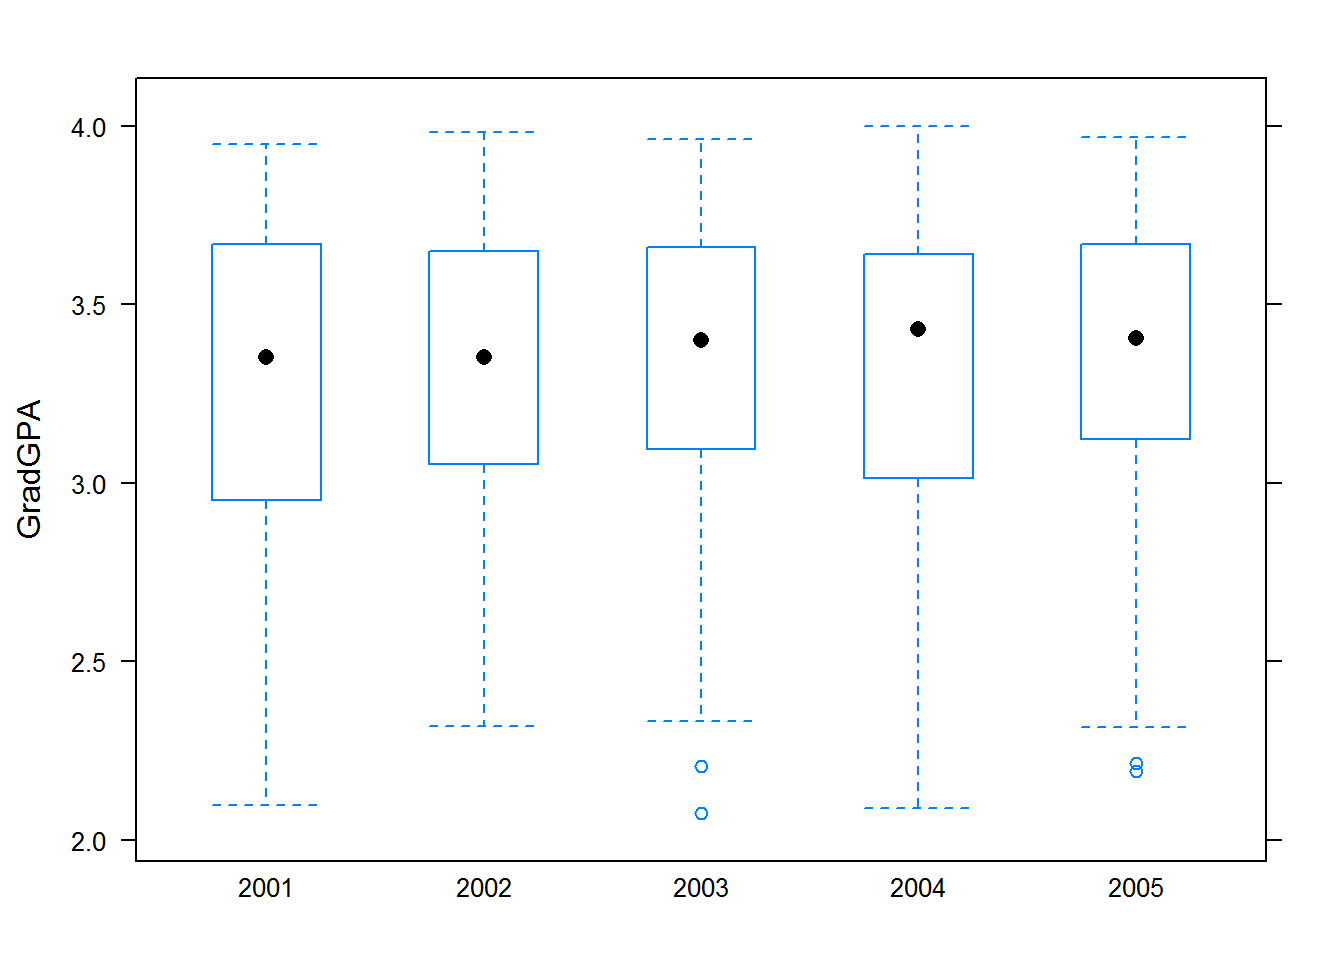
\includegraphics{fastR-Notes_files/figure-latex/unnamed-chunk-28-1.pdf}

Now you investigate the height data we took in class.

\begin{Shaded}
\begin{Highlighting}[]
\NormalTok{Lesson2_Data <-}\StringTok{ }\KeywordTok{read.csv}\NormalTok{(}\StringTok{"Lesson2_Height.csv"}\NormalTok{)}
\end{Highlighting}
\end{Shaded}

\begin{Shaded}
\begin{Highlighting}[]
\KeywordTok{str}\NormalTok{(Lesson2_Data)}
\end{Highlighting}
\end{Shaded}

\begin{verbatim}
## 'data.frame':    25 obs. of  2 variables:
##  $ Gender: Factor w/ 2 levels "Female","Male": 2 2 2 2 2 2 2 2 2 2 ...
##  $ Height: num  69 78 77 64.5 67 72 72 67 75 77 ...
\end{verbatim}

\begin{Shaded}
\begin{Highlighting}[]
\KeywordTok{summary}\NormalTok{(Lesson2_Data)}
\end{Highlighting}
\end{Shaded}

\begin{verbatim}
##     Gender       Height     
##  Female: 8   Min.   :62.50  
##  Male  :17   1st Qu.:67.00  
##              Median :70.00  
##              Mean   :70.14  
##              3rd Qu.:73.00  
##              Max.   :78.00
\end{verbatim}

\begin{Shaded}
\begin{Highlighting}[]
\KeywordTok{bwplot}\NormalTok{(}\OperatorTok{~}\NormalTok{Height,Lesson2_Data)}
\end{Highlighting}
\end{Shaded}

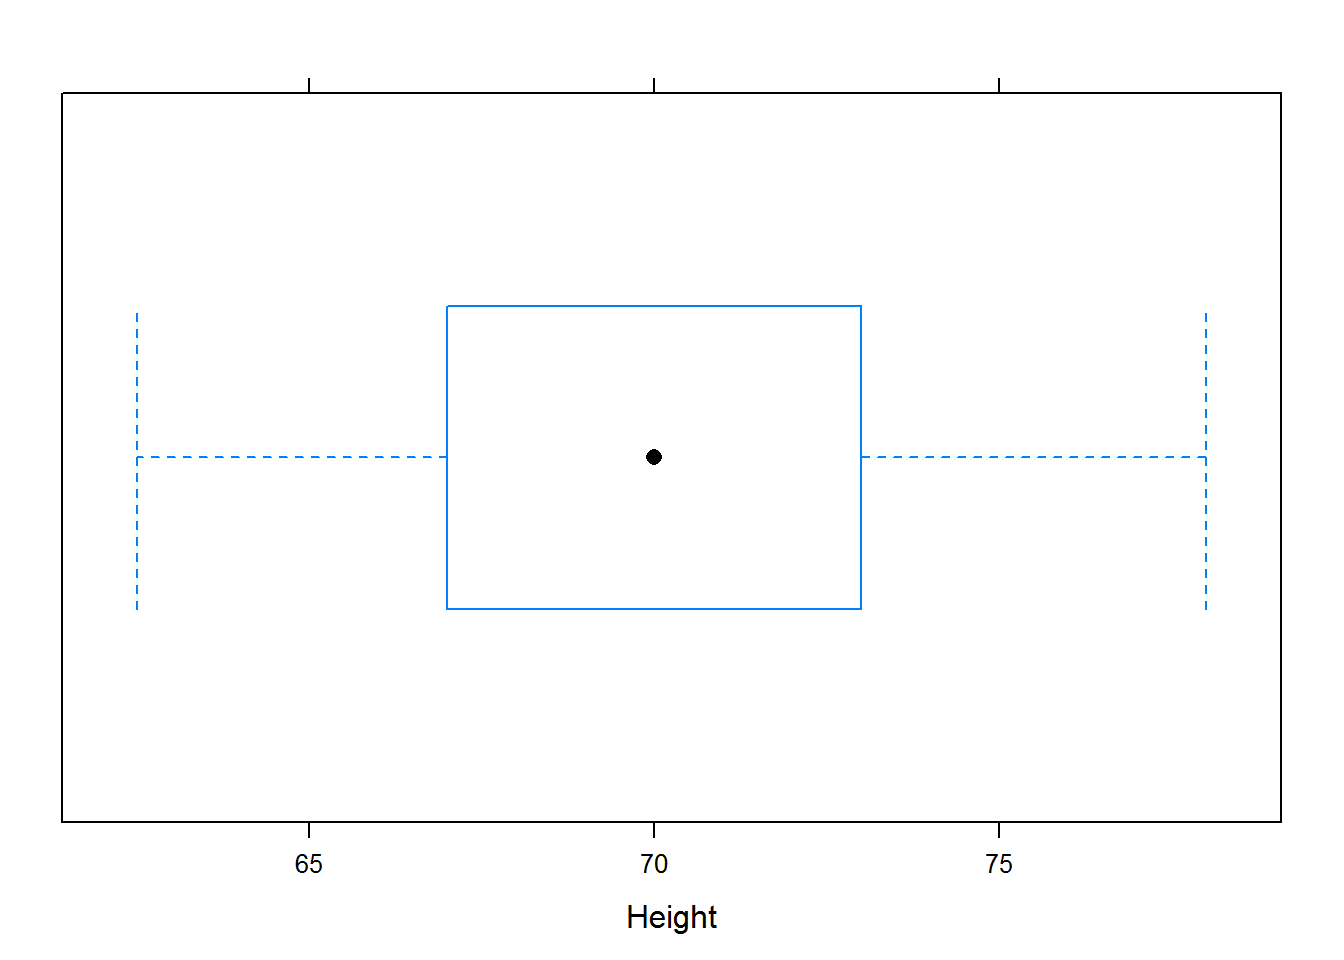
\includegraphics{fastR-Notes_files/figure-latex/unnamed-chunk-32-1.pdf}

\begin{Shaded}
\begin{Highlighting}[]
\KeywordTok{bwplot}\NormalTok{(Height}\OperatorTok{~}\NormalTok{Gender,Lesson2_Data)}
\end{Highlighting}
\end{Shaded}

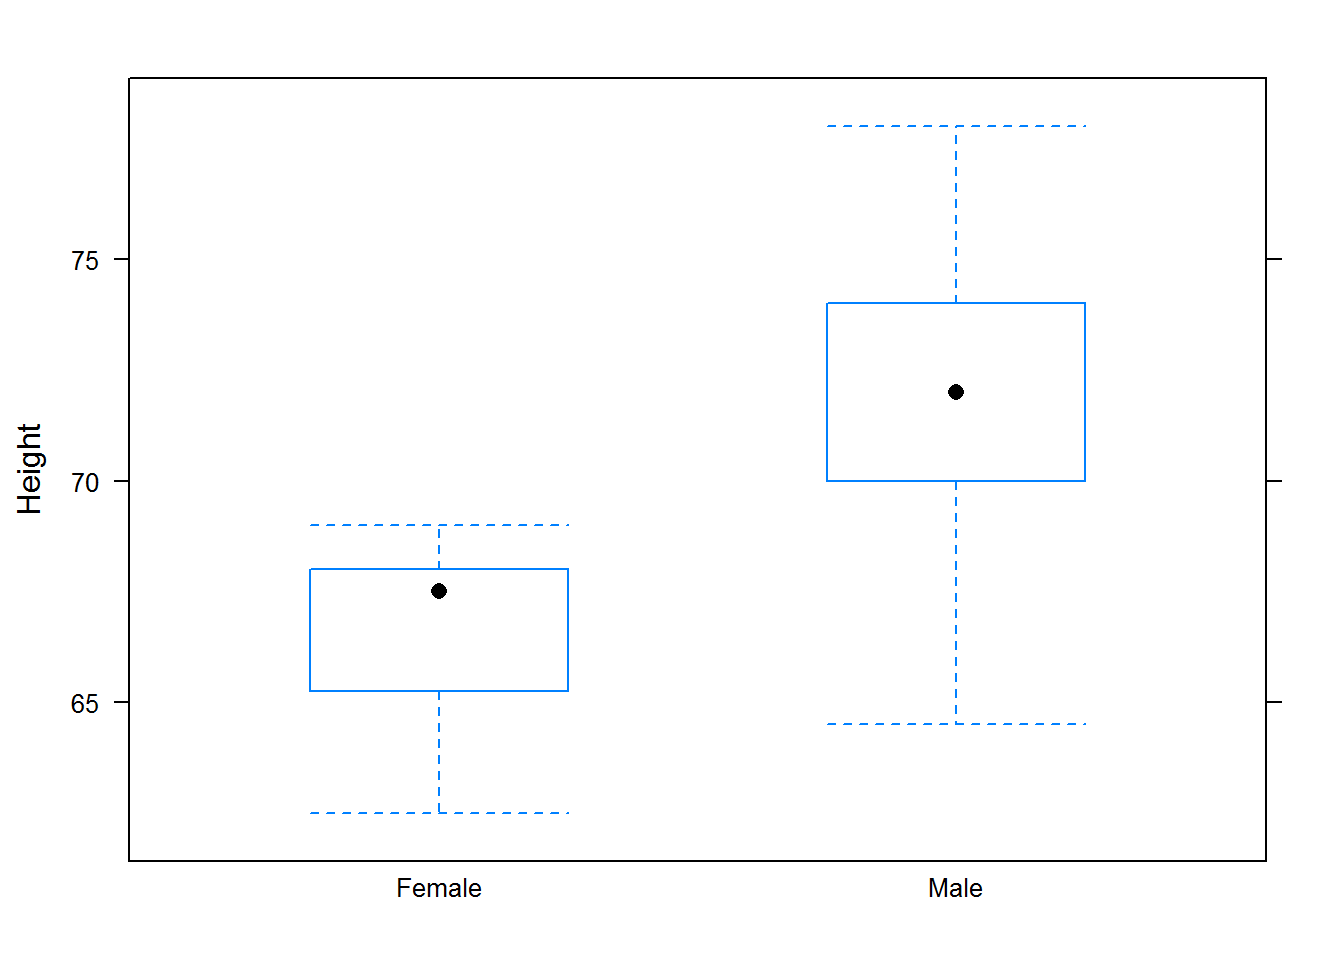
\includegraphics{fastR-Notes_files/figure-latex/unnamed-chunk-33-1.pdf}

\begin{Shaded}
\begin{Highlighting}[]
\KeywordTok{summary}\NormalTok{(Height}\OperatorTok{~}\NormalTok{Gender,}\DataTypeTok{data=}\NormalTok{Lesson2_Data,}\DataTypeTok{fun=}\NormalTok{favstats)}
\end{Highlighting}
\end{Shaded}

\begin{verbatim}
## Height     N= 25 
## 
## +-------+------+--+----+------+-------+---+----+--------+--------+--+--------+
## |       |      |N |min |Q1    |median |Q3 |max |mean    |sd      |n |missing |
## +-------+------+--+----+------+-------+---+----+--------+--------+--+--------+
## |Gender |Female| 8|62.5|65.875|67.5   |68 |69  |66.62500|2.248015| 8|0       |
## |       |Male  |17|64.5|70.000|72.0   |74 |78  |71.79412|3.804023|17|0       |
## +-------+------+--+----+------+-------+---+----+--------+--------+--+--------+
## |Overall|      |25|62.5|67.000|70.0   |73 |78  |70.14000|4.144575|25|0       |
## +-------+------+--+----+------+-------+---+----+--------+--------+--+--------+
\end{verbatim}

\hypertarget{L3}{\section{Summarizing Multivariate Data}\label{L3}}

\subsection{Objectives}\label{objectives-2}

\begin{enumerate}
\def\labelenumi{\arabic{enumi}.}
\tightlist
\item
  Understand model notation by using in R
\item
  Distinguish between variable types (nominal, ordinal, and continuous)
  and give examples
\item
  Develop a framework and use to create numeric and visual summaries of
  bivariate data
\item
  Explain lurking variable
\end{enumerate}

\subsection{Ideas from last lesson}\label{ideas-from-last-lesson}

In \ref{Les2} we discussed the idea of symmetry. Symmetry and the idea
on equality of mean and median depend on definition of symmetric. Some
basic definitions of symmetry are simply that the mean and median are
equal. However, page 22 of the book has a different definition of
symmetry. This second definition is more accurate and will be easier to
understand when we introduce probability density functions.

Using the second definition, if a distribution is symmetric, then the
mean and median are equal. However, if the mean and median are equal,
then the distribution does not have to be symmetric.

Consider the following data set:

\begin{Shaded}
\begin{Highlighting}[]
\NormalTok{Les3_ex<-}\KeywordTok{c}\NormalTok{(}\OperatorTok{-}\DecValTok{2}\NormalTok{,}\DecValTok{4}\NormalTok{,}\DecValTok{5}\NormalTok{,}\DecValTok{8}\NormalTok{,}\DecValTok{10}\NormalTok{)}
\end{Highlighting}
\end{Shaded}

\begin{Shaded}
\begin{Highlighting}[]
\KeywordTok{summary}\NormalTok{(Les3_ex)}
\end{Highlighting}
\end{Shaded}

\begin{verbatim}
##    Min. 1st Qu.  Median    Mean 3rd Qu.    Max. 
##      -2       4       5       5       8      10
\end{verbatim}

From last class, what would be the difference between

\begin{verbatim}
bwplot(Height~Gender,Lesson2_Data)
\end{verbatim}

and

\begin{verbatim}
bwplot(~Height|Gender,Lesson2_Data)
\end{verbatim}

Is class year qualitative or quantitative?

Homework 1.10 Try it.

\subsection{Bivariate Data}\label{bivariate-data}

Load libraries

\begin{Shaded}
\begin{Highlighting}[]
\KeywordTok{library}\NormalTok{(}\StringTok{'fastR'}\NormalTok{)}
\KeywordTok{library}\NormalTok{(Hmisc)}
\KeywordTok{library}\NormalTok{(lattice)}
\KeywordTok{library}\NormalTok{(vcd)}
\end{Highlighting}
\end{Shaded}

Bivariate data means that we have two variables. There are three
possibilities, in the next chapter will cover the idea of counting but
here we are sampling with replacement and order does not matter. We
could have two qualitative variables, one qualitative and one
quantitative, and finally two quantitative.

Qualitative variables are often the most difficult to look at. Last
lesson we looked at one variable being qualitative and the other being
quantitative. We created side-by-side plots and summary statistics by
categories of the qualitative variable.

Now, let's look at two qualitative variables. Use the data set
airlineArrival for this analysis.

\begin{Shaded}
\begin{Highlighting}[]
\KeywordTok{str}\NormalTok{(airlineArrival)}
\end{Highlighting}
\end{Shaded}

\begin{verbatim}
## 'data.frame':    11000 obs. of  3 variables:
##  $ Airport: Factor w/ 5 levels "LosAngeles","Phoenix",..: 2 4 4 4 2 1 2 2 5 5 ...
##  $ Result : Factor w/ 2 levels "Delayed","OnTime": 2 2 2 2 2 2 2 2 2 2 ...
##  $ Airline: Factor w/ 2 levels "Alaska","AmericaWest": 2 1 1 1 2 1 2 2 1 1 ...
\end{verbatim}

Summarize in a table

\begin{Shaded}
\begin{Highlighting}[]
\KeywordTok{xtabs}\NormalTok{(}\OperatorTok{~}\NormalTok{Result}\OperatorTok{+}\NormalTok{Airline,}\DataTypeTok{data=}\NormalTok{airlineArrival)}
\end{Highlighting}
\end{Shaded}

\begin{verbatim}
##          Airline
## Result    Alaska AmericaWest
##   Delayed    501         787
##   OnTime    3274        6438
\end{verbatim}

Often you can do things several ways in R

\begin{Shaded}
\begin{Highlighting}[]
\KeywordTok{table}\NormalTok{(airlineArrival[,}\DecValTok{2}\OperatorTok{:}\DecValTok{3}\NormalTok{])}
\end{Highlighting}
\end{Shaded}

\begin{verbatim}
##          Airline
## Result    Alaska AmericaWest
##   Delayed    501         787
##   OnTime    3274        6438
\end{verbatim}

\begin{Shaded}
\begin{Highlighting}[]
\KeywordTok{table}\NormalTok{(airlineArrival}\OperatorTok{$}\NormalTok{Result,airlineArrival}\OperatorTok{$}\NormalTok{Airline)}
\end{Highlighting}
\end{Shaded}

\begin{verbatim}
##          
##           Alaska AmericaWest
##   Delayed    501         787
##   OnTime    3274        6438
\end{verbatim}

If we want proportion, we can use

\begin{Shaded}
\begin{Highlighting}[]
\KeywordTok{prop.table}\NormalTok{(}\KeywordTok{table}\NormalTok{(airlineArrival[,}\DecValTok{2}\OperatorTok{:}\DecValTok{3}\NormalTok{]),}\DecValTok{2}\NormalTok{)}
\end{Highlighting}
\end{Shaded}

\begin{verbatim}
##          Airline
## Result       Alaska AmericaWest
##   Delayed 0.1327152   0.1089273
##   OnTime  0.8672848   0.8910727
\end{verbatim}

Why not the following?

\begin{Shaded}
\begin{Highlighting}[]
\KeywordTok{prop.table}\NormalTok{(}\KeywordTok{table}\NormalTok{(airlineArrival[,}\DecValTok{2}\OperatorTok{:}\DecValTok{3}\NormalTok{])) }\CommentTok{#not what we want}
\end{Highlighting}
\end{Shaded}

\begin{verbatim}
##          Airline
## Result        Alaska AmericaWest
##   Delayed 0.04554545  0.07154545
##   OnTime  0.29763636  0.58527273
\end{verbatim}

In this problem we can look at the variable result depending on the
airline. Thus we summarize the data differently than if both variables
were thought of being independent. We will see this more in chapter 4.

There is a plot method called \texttt{mosiac}. Be careful using this
because it uses areas and we are not good at visually comparing areas,
thus avoid pie charts. The function is in the \texttt{vcd} package.

\begin{verbatim}
require(vcd)
mosaic(~Result+Airline,airlineArrival) # This is the wrong plot why?
\end{verbatim}

Better plot is

\begin{Shaded}
\begin{Highlighting}[]
\KeywordTok{mosaic}\NormalTok{(Result}\OperatorTok{~}\NormalTok{Airline,airlineArrival)}
\end{Highlighting}
\end{Shaded}

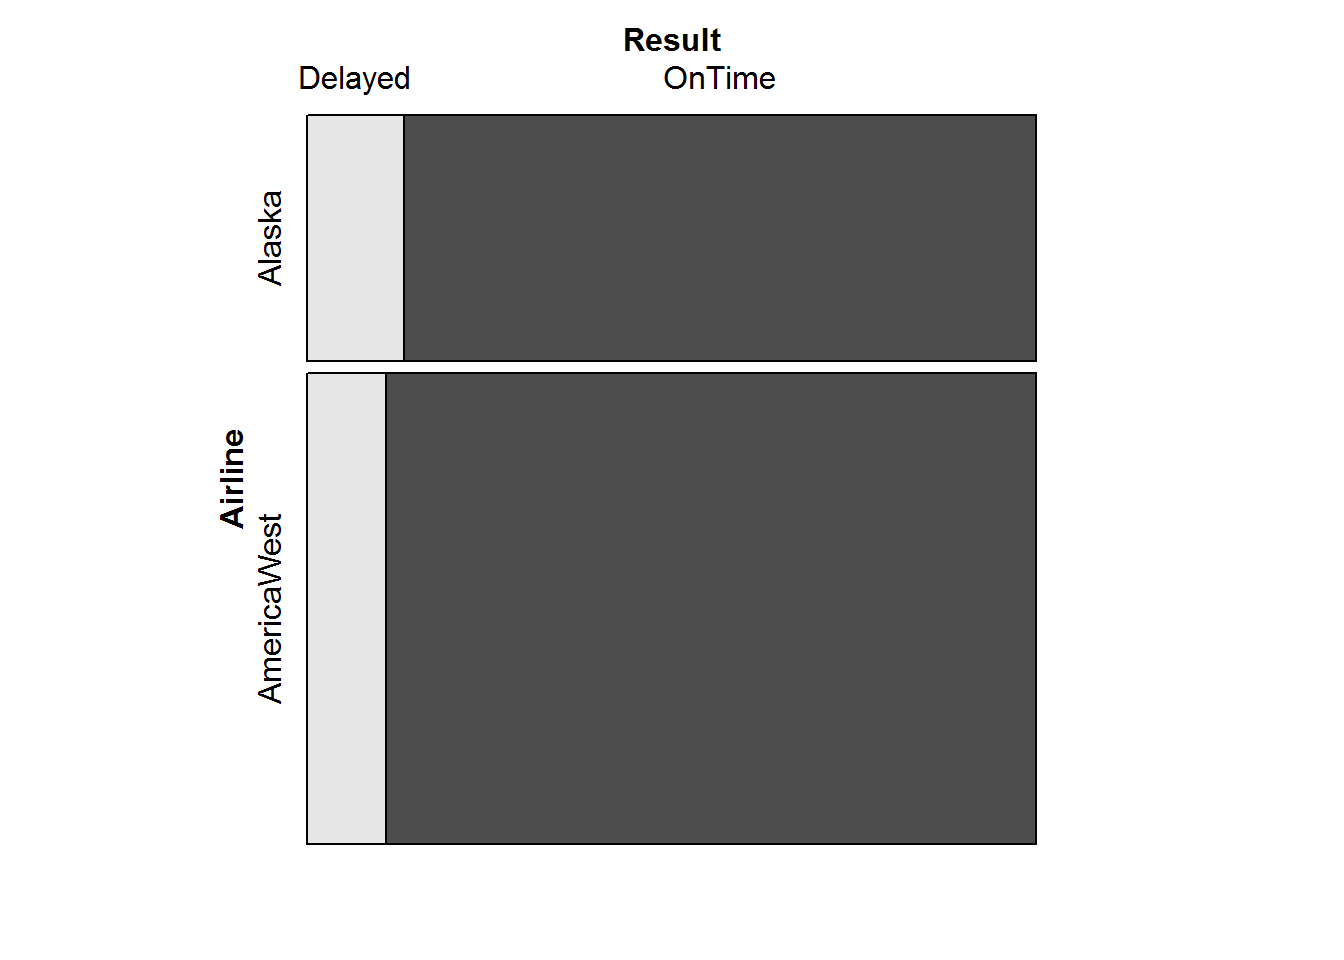
\includegraphics{fastR-Notes_files/figure-latex/unnamed-chunk-43-1.pdf}

Looks like AmericaWest is the better airline because it has a higher
proportion of the plans arrive on time. But wait.

Let's break it down by airport.

\begin{Shaded}
\begin{Highlighting}[]
\KeywordTok{structable}\NormalTok{(}\OperatorTok{~}\NormalTok{Result}\OperatorTok{+}\NormalTok{Airline}\OperatorTok{+}\NormalTok{Airport,airlineArrival)}
\end{Highlighting}
\end{Shaded}

\begin{verbatim}
##                      Airline Alaska AmericaWest
## Result  Airport                                
## Delayed LosAngeles               62         117
##         Phoenix                  12         415
##         SanDiego                 20          65
##         SanFrancisco            102         129
##         Seattle                 305          61
## OnTime  LosAngeles              497         694
##         Phoenix                 221        4840
##         SanDiego                212         383
##         SanFrancisco            503         320
##         Seattle                1841         201
\end{verbatim}

This is too hard to read, so look at this result:

\begin{Shaded}
\begin{Highlighting}[]
\KeywordTok{prop.table}\NormalTok{(}\KeywordTok{table}\NormalTok{(airlineArrival),}\KeywordTok{c}\NormalTok{(}\DecValTok{1}\NormalTok{,}\DecValTok{3}\NormalTok{))}
\end{Highlighting}
\end{Shaded}

\begin{verbatim}
## , , Airline = Alaska
## 
##               Result
## Airport           Delayed     OnTime
##   LosAngeles   0.11091234 0.88908766
##   Phoenix      0.05150215 0.94849785
##   SanDiego     0.08620690 0.91379310
##   SanFrancisco 0.16859504 0.83140496
##   Seattle      0.14212488 0.85787512
## 
## , , Airline = AmericaWest
## 
##               Result
## Airport           Delayed     OnTime
##   LosAngeles   0.14426634 0.85573366
##   Phoenix      0.07897241 0.92102759
##   SanDiego     0.14508929 0.85491071
##   SanFrancisco 0.28730512 0.71269488
##   Seattle      0.23282443 0.76717557
\end{verbatim}

It looks like for every airport, Alaska has a better on time rate than
AmericaWest. How come AmericaWest has the overall better on time rate?

See this site for another example of
\href{http://vudlab.com/simpsons/}{Simpson's Paradox} and the idea of a
lurking variable.

The following is a plot but I don't like it as much as a table.

\begin{Shaded}
\begin{Highlighting}[]
\KeywordTok{mosaic}\NormalTok{(Result}\OperatorTok{~}\NormalTok{Airline}\OperatorTok{+}\NormalTok{Airport,airlineArrival)}
\end{Highlighting}
\end{Shaded}

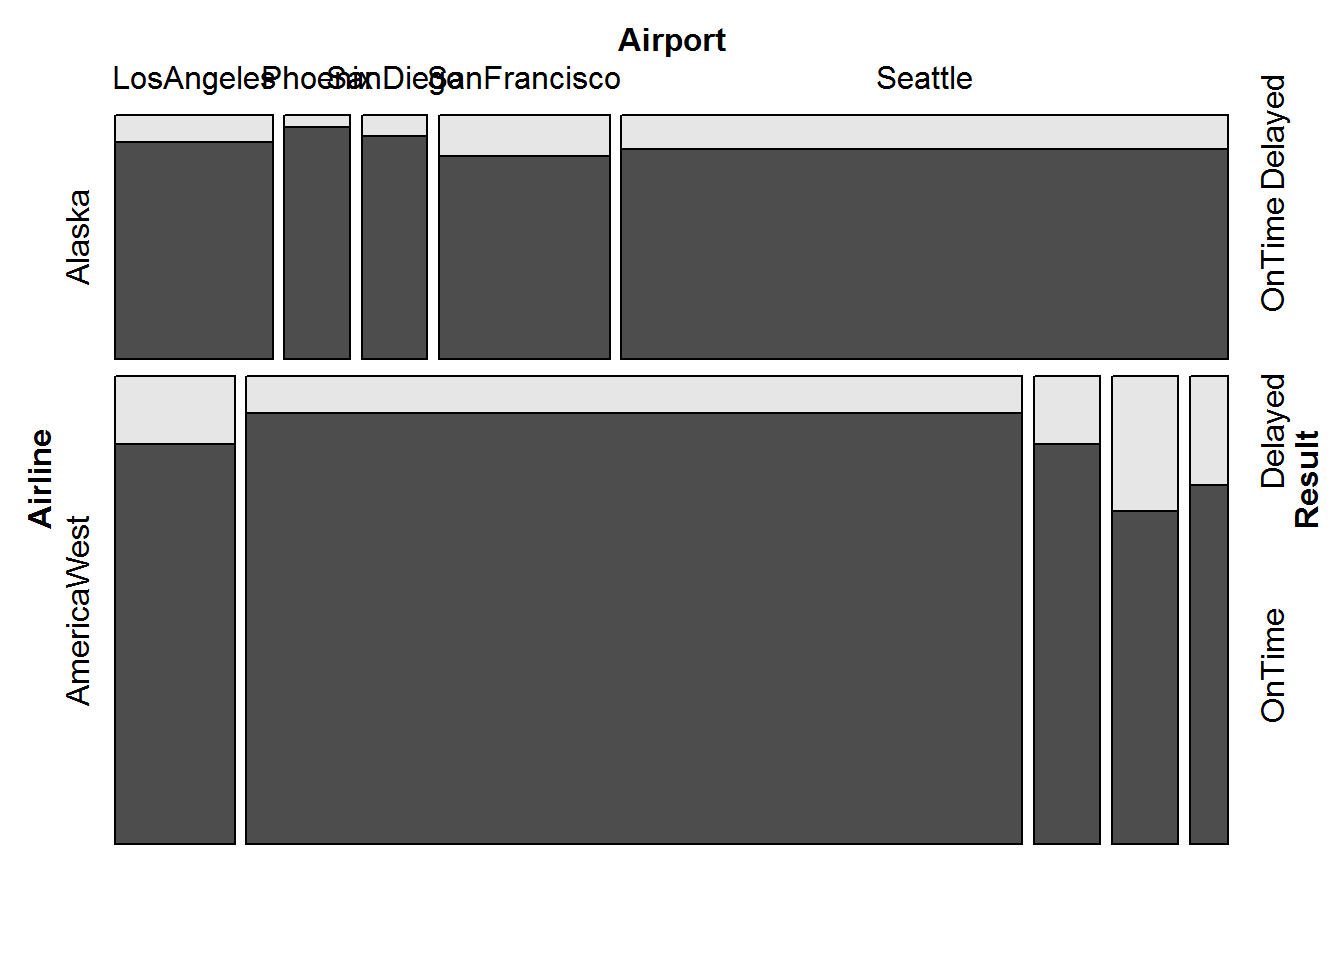
\includegraphics{fastR-Notes_files/figure-latex/unnamed-chunk-46-1.pdf}

Bivariate with both quantitative leads to the familiar scatterplot. The
book's example on the iris data set is good.

In that case they add a third qualitative variable and use color via the
groups option to visualize.

Some more examples

\begin{Shaded}
\begin{Highlighting}[]
\KeywordTok{names}\NormalTok{(students)}
\end{Highlighting}
\end{Shaded}

\begin{verbatim}
## [1] "ACT"     "SAT"     "Grad"    "GradGPA" "HSGPA"   "Cohort"
\end{verbatim}

\begin{Shaded}
\begin{Highlighting}[]
\KeywordTok{table}\NormalTok{(students}\OperatorTok{$}\NormalTok{Cohort,students}\OperatorTok{$}\NormalTok{Grad)}
\end{Highlighting}
\end{Shaded}

\begin{verbatim}
##       
##        FALSE TRUE
##   2001    58  142
##   2002    43  178
##   2003    50  154
##   2004    47  140
##   2005    70  118
\end{verbatim}

\begin{Shaded}
\begin{Highlighting}[]
\KeywordTok{xtabs}\NormalTok{(}\OperatorTok{~}\NormalTok{Cohort}\OperatorTok{+}\NormalTok{Grad,students)}
\end{Highlighting}
\end{Shaded}

\begin{verbatim}
##       Grad
## Cohort FALSE TRUE
##   2001    58  142
##   2002    43  178
##   2003    50  154
##   2004    47  140
##   2005    70  118
\end{verbatim}

\begin{Shaded}
\begin{Highlighting}[]
\KeywordTok{histogram}\NormalTok{(}\OperatorTok{~}\NormalTok{GradGPA}\OperatorTok{|}\KeywordTok{factor}\NormalTok{(Cohort),students)}
\end{Highlighting}
\end{Shaded}

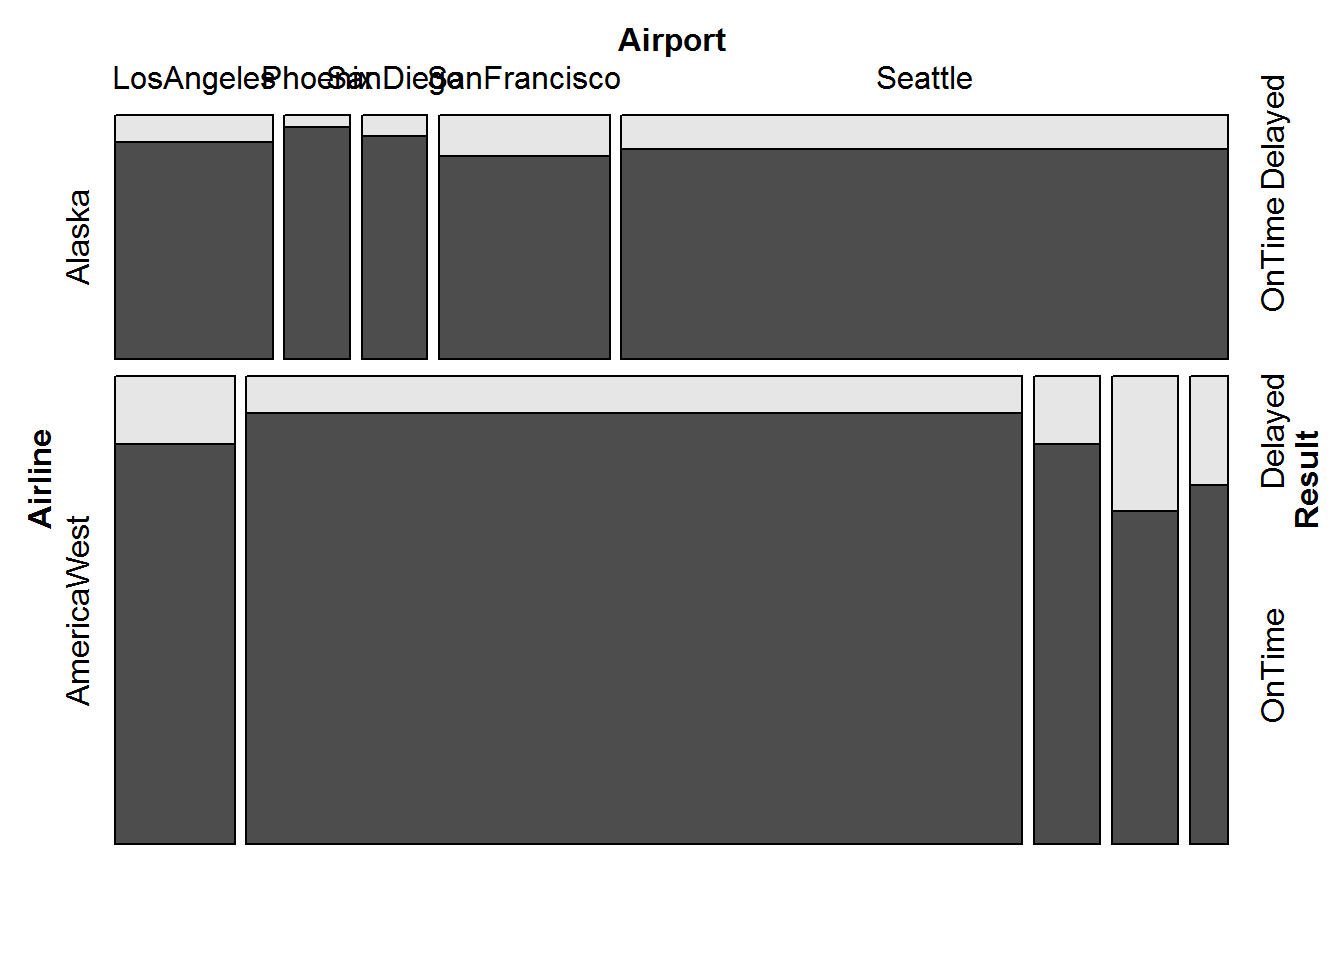
\includegraphics{fastR-Notes_files/figure-latex/unnamed-chunk-48-1.pdf}

\begin{Shaded}
\begin{Highlighting}[]
\KeywordTok{bwplot}\NormalTok{(}\OperatorTok{~}\NormalTok{GradGPA}\OperatorTok{|}\KeywordTok{factor}\NormalTok{(Cohort),students)}
\end{Highlighting}
\end{Shaded}

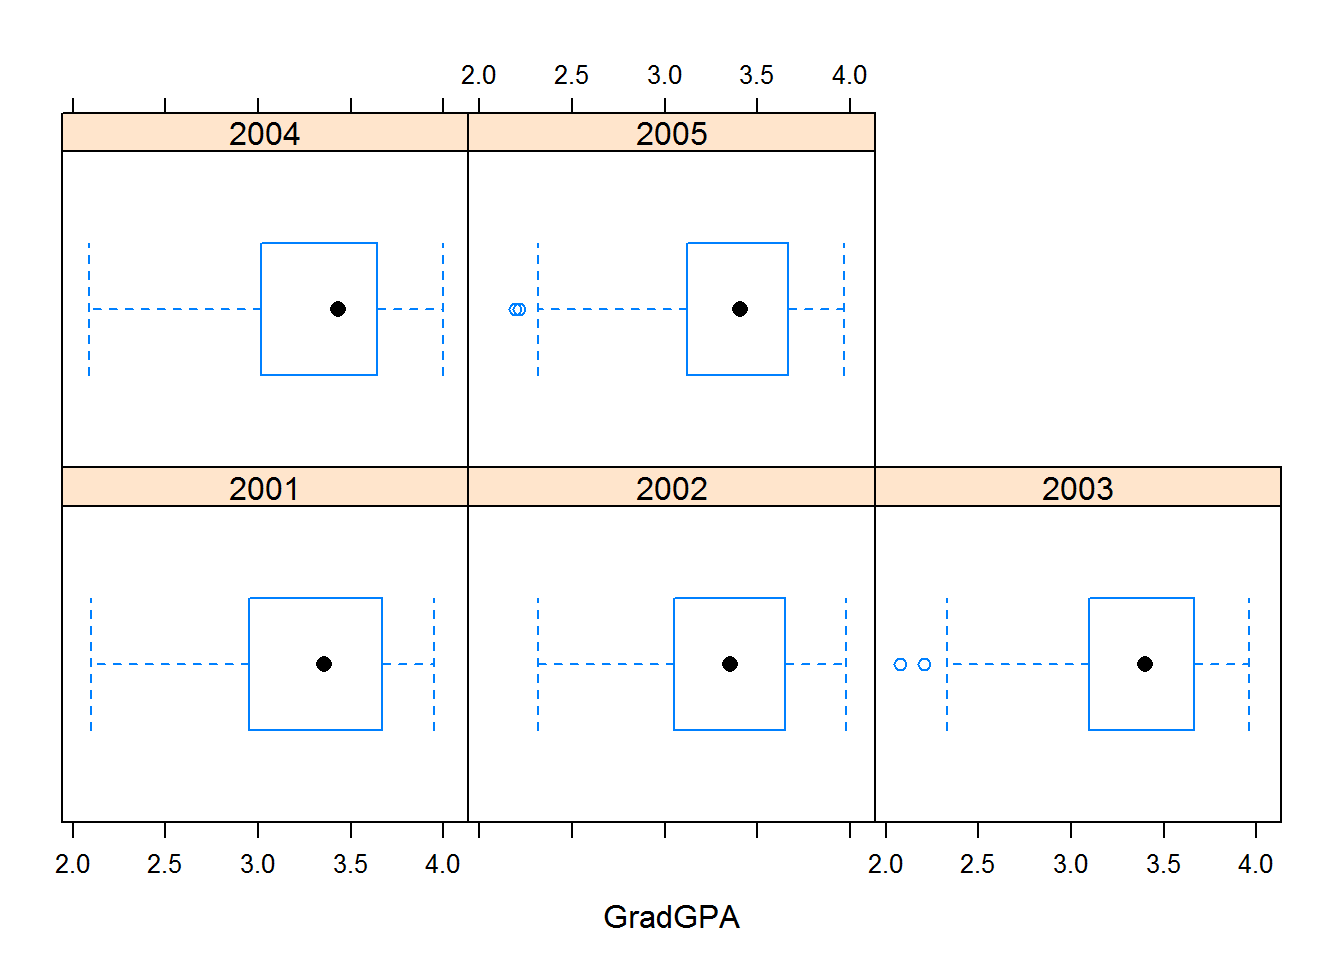
\includegraphics{fastR-Notes_files/figure-latex/unnamed-chunk-49-1.pdf}

\begin{Shaded}
\begin{Highlighting}[]
\KeywordTok{bwplot}\NormalTok{(GradGPA}\OperatorTok{~}\KeywordTok{factor}\NormalTok{(Cohort),students)}
\end{Highlighting}
\end{Shaded}

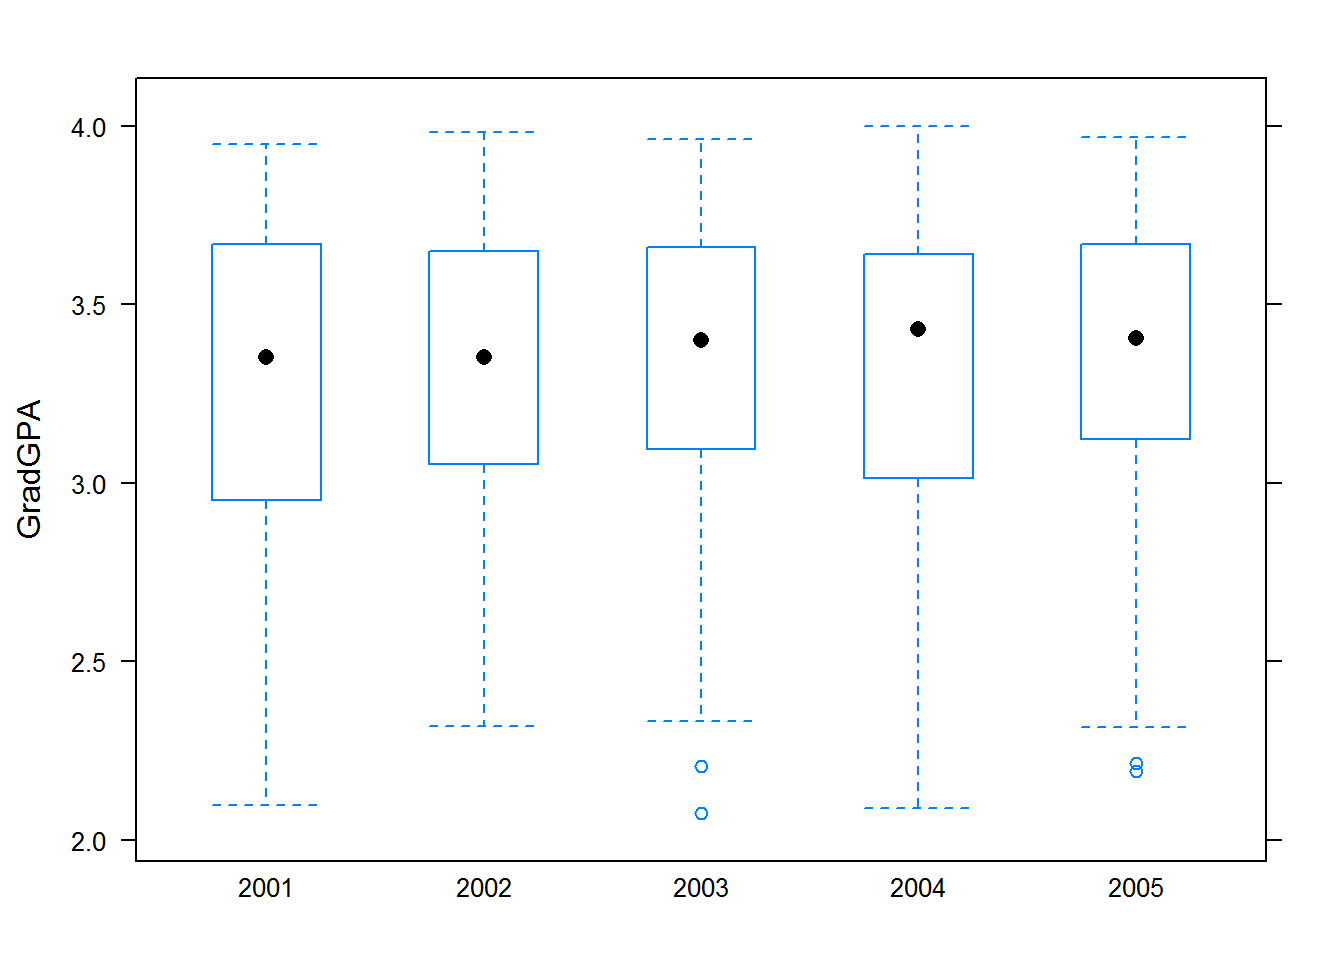
\includegraphics{fastR-Notes_files/figure-latex/unnamed-chunk-49-2.pdf}

\begin{Shaded}
\begin{Highlighting}[]
\KeywordTok{xyplot}\NormalTok{(GradGPA}\OperatorTok{~}\NormalTok{HSGPA,students)}
\end{Highlighting}
\end{Shaded}

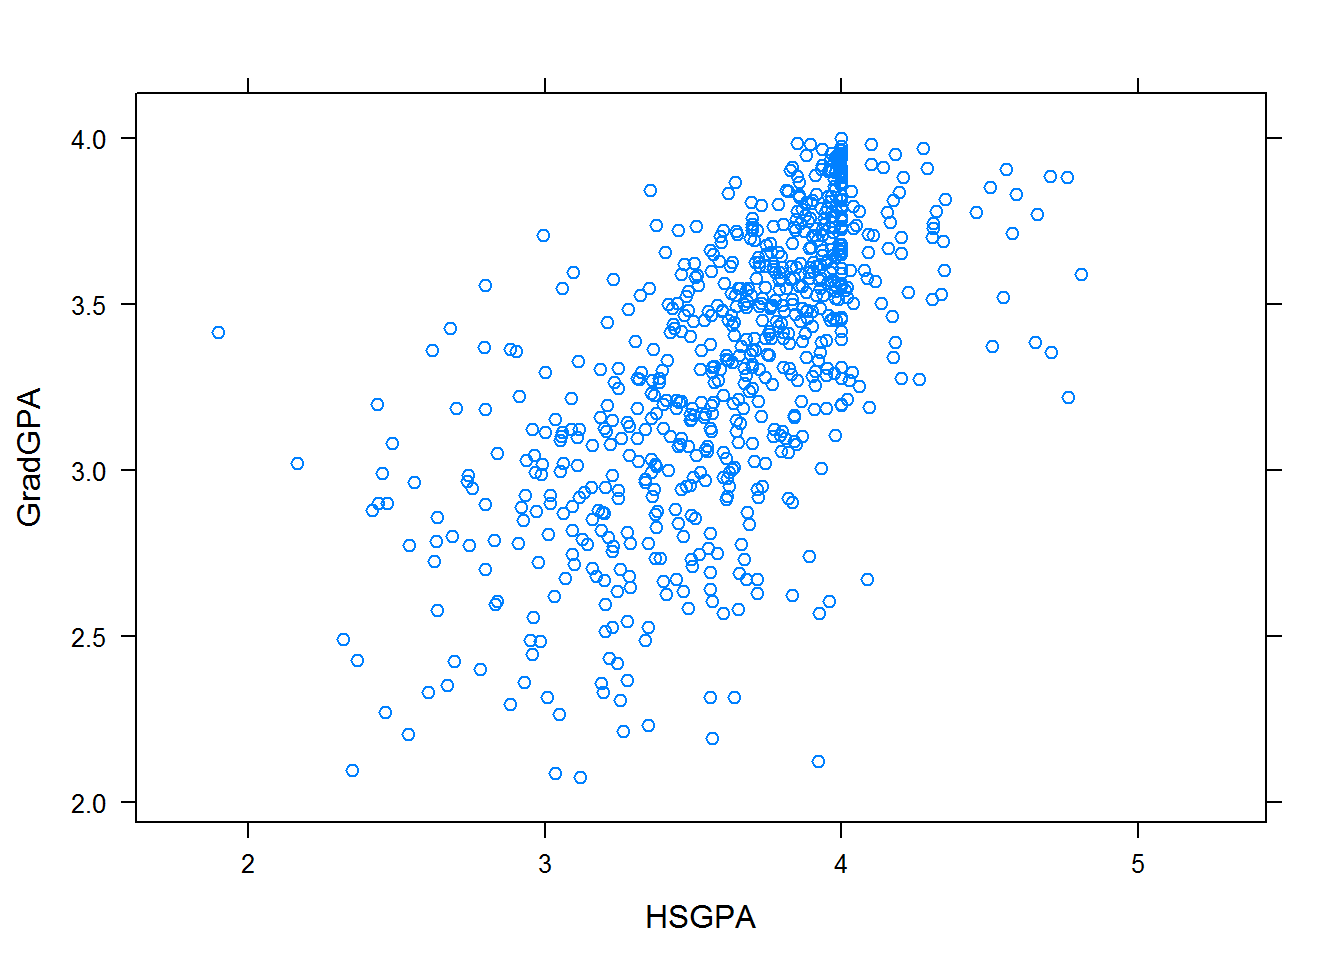
\includegraphics{fastR-Notes_files/figure-latex/unnamed-chunk-50-1.pdf}

\begin{Shaded}
\begin{Highlighting}[]
\KeywordTok{xyplot}\NormalTok{(GradGPA}\OperatorTok{~}\NormalTok{HSGPA,students,}\DataTypeTok{main=}\StringTok{"Lesson 3 Example"}\NormalTok{)}
\end{Highlighting}
\end{Shaded}

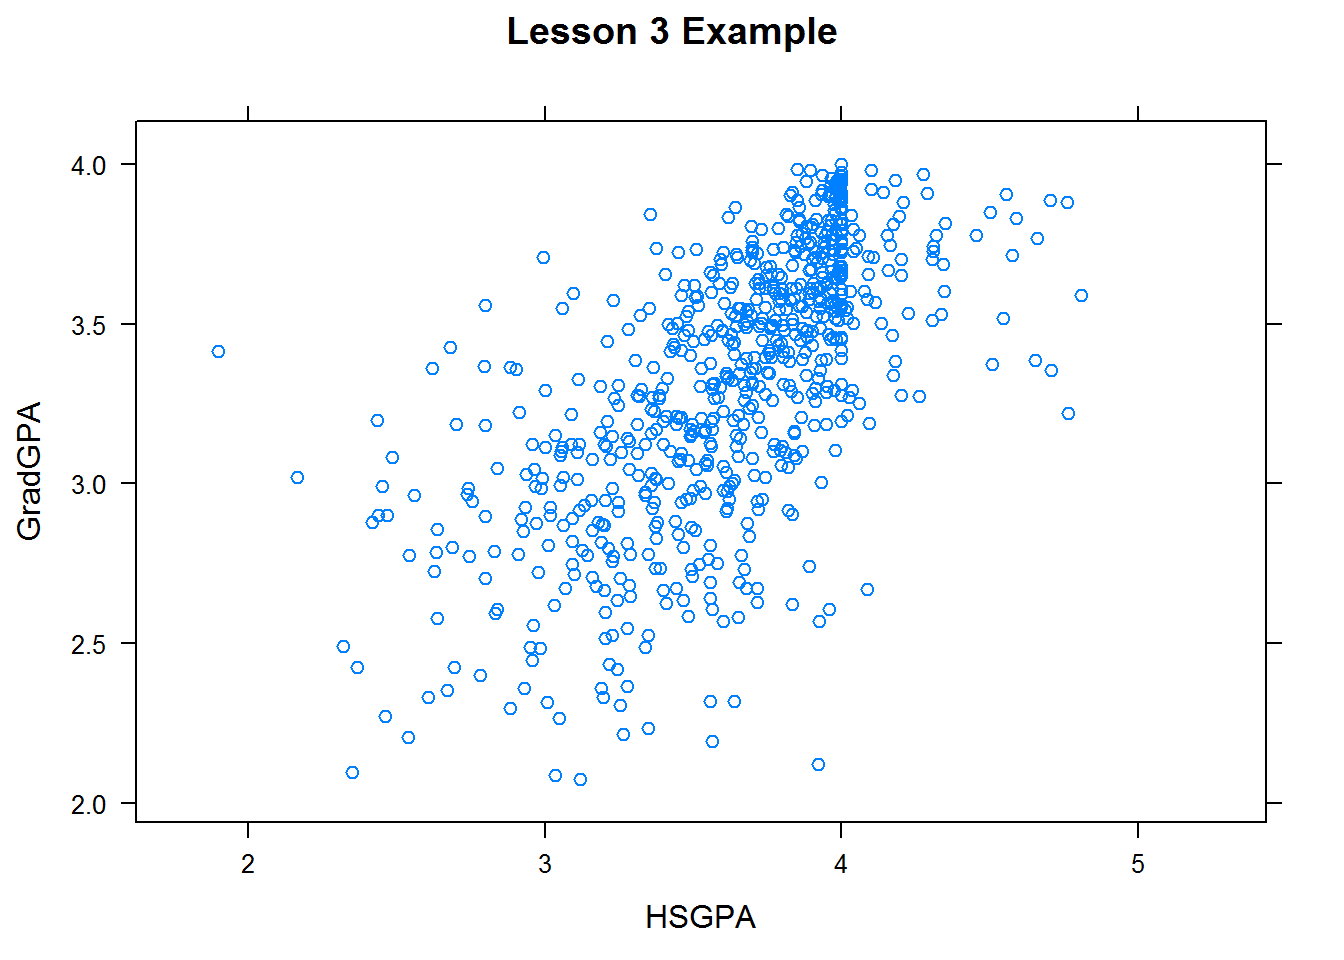
\includegraphics{fastR-Notes_files/figure-latex/unnamed-chunk-50-2.pdf}

\begin{Shaded}
\begin{Highlighting}[]
\KeywordTok{xyplot}\NormalTok{(GradGPA}\OperatorTok{~}\NormalTok{HSGPA,}\DataTypeTok{group=}\NormalTok{Cohort,students,}\DataTypeTok{main=}\StringTok{"Lesson 3 Example"}\NormalTok{,}\DataTypeTok{auto.key=}\NormalTok{T)}
\end{Highlighting}
\end{Shaded}

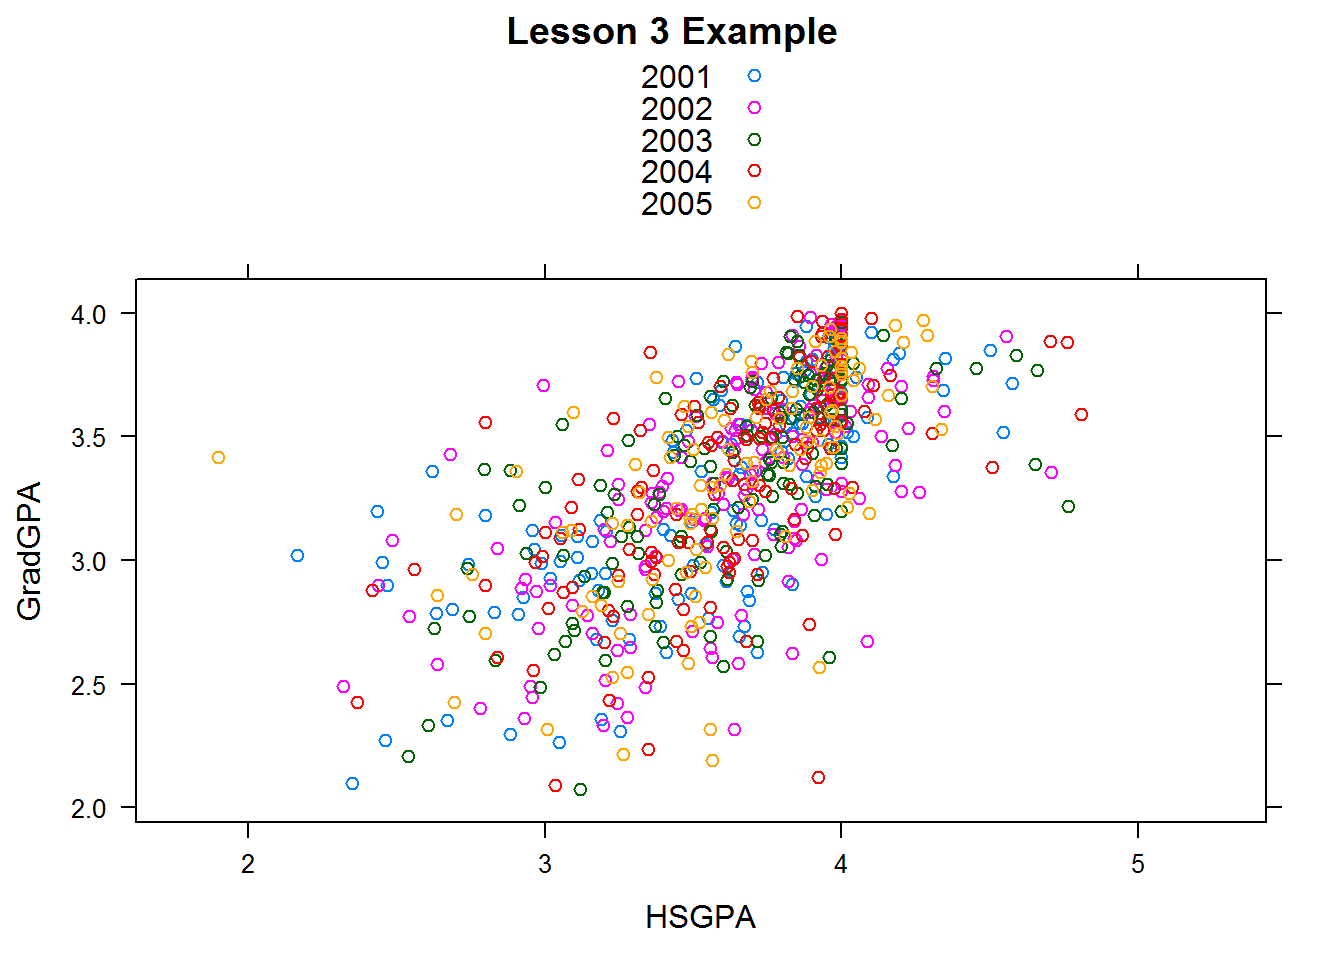
\includegraphics{fastR-Notes_files/figure-latex/unnamed-chunk-50-3.pdf}

\begin{Shaded}
\begin{Highlighting}[]
\KeywordTok{xyplot}\NormalTok{(GradGPA}\OperatorTok{~}\NormalTok{HSGPA}\OperatorTok{|}\NormalTok{Cohort,students,}\DataTypeTok{main=}\StringTok{"Lesson 3 Example"}\NormalTok{)}
\end{Highlighting}
\end{Shaded}

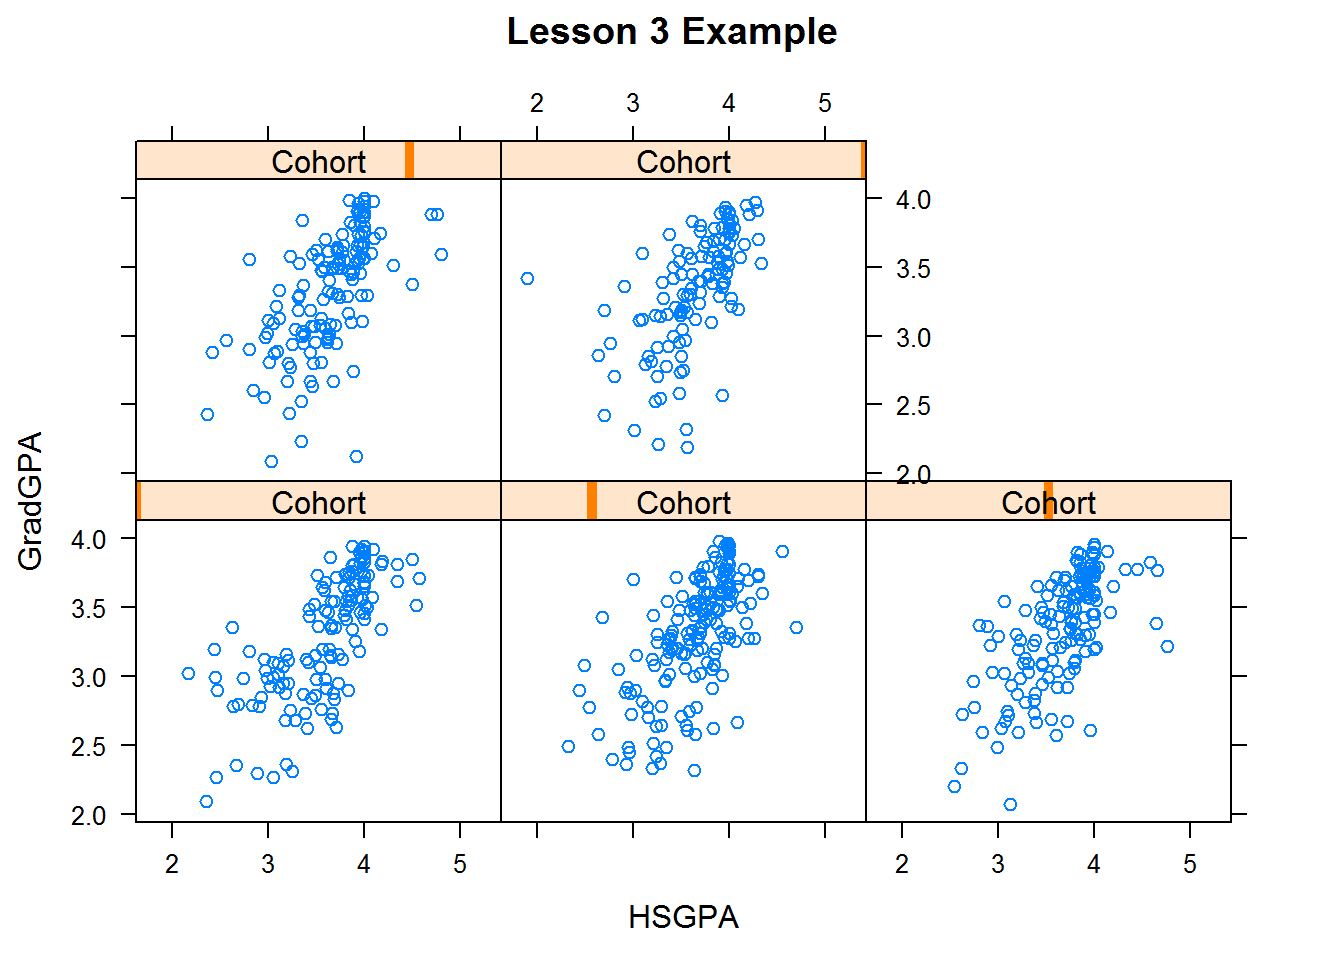
\includegraphics{fastR-Notes_files/figure-latex/unnamed-chunk-50-4.pdf}

\begin{Shaded}
\begin{Highlighting}[]
\KeywordTok{xyplot}\NormalTok{(GradGPA}\OperatorTok{~}\NormalTok{HSGPA}\OperatorTok{|}\KeywordTok{factor}\NormalTok{(Cohort),students,}\DataTypeTok{main=}\StringTok{"Lesson 3 Example"}\NormalTok{)}
\end{Highlighting}
\end{Shaded}

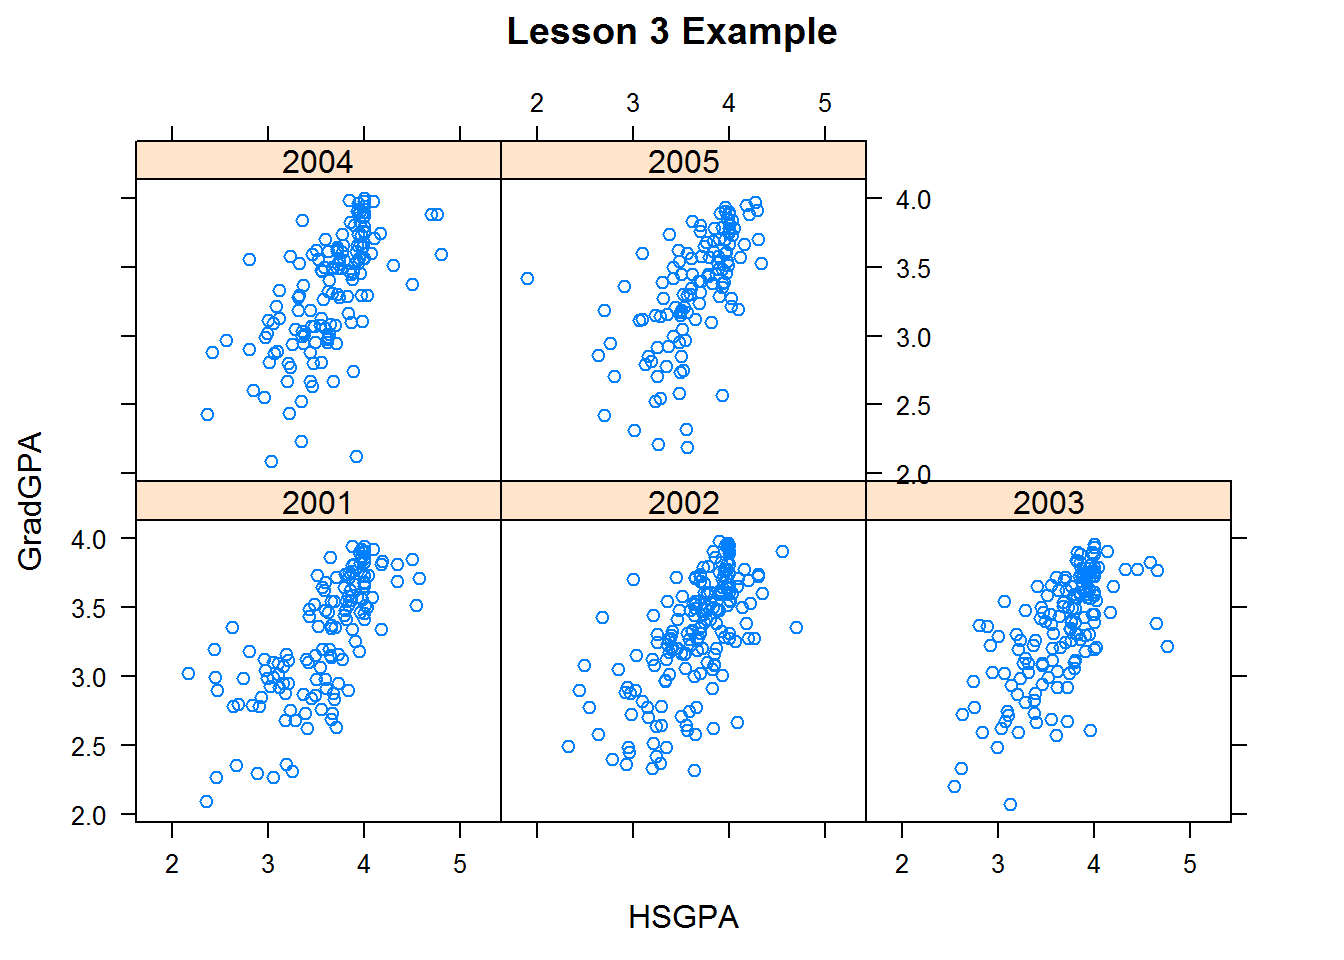
\includegraphics{fastR-Notes_files/figure-latex/unnamed-chunk-50-5.pdf}

\begin{Shaded}
\begin{Highlighting}[]
\KeywordTok{plot}\NormalTok{(students}\OperatorTok{$}\NormalTok{HSGPA,students}\OperatorTok{$}\NormalTok{GradGPA)}
\end{Highlighting}
\end{Shaded}

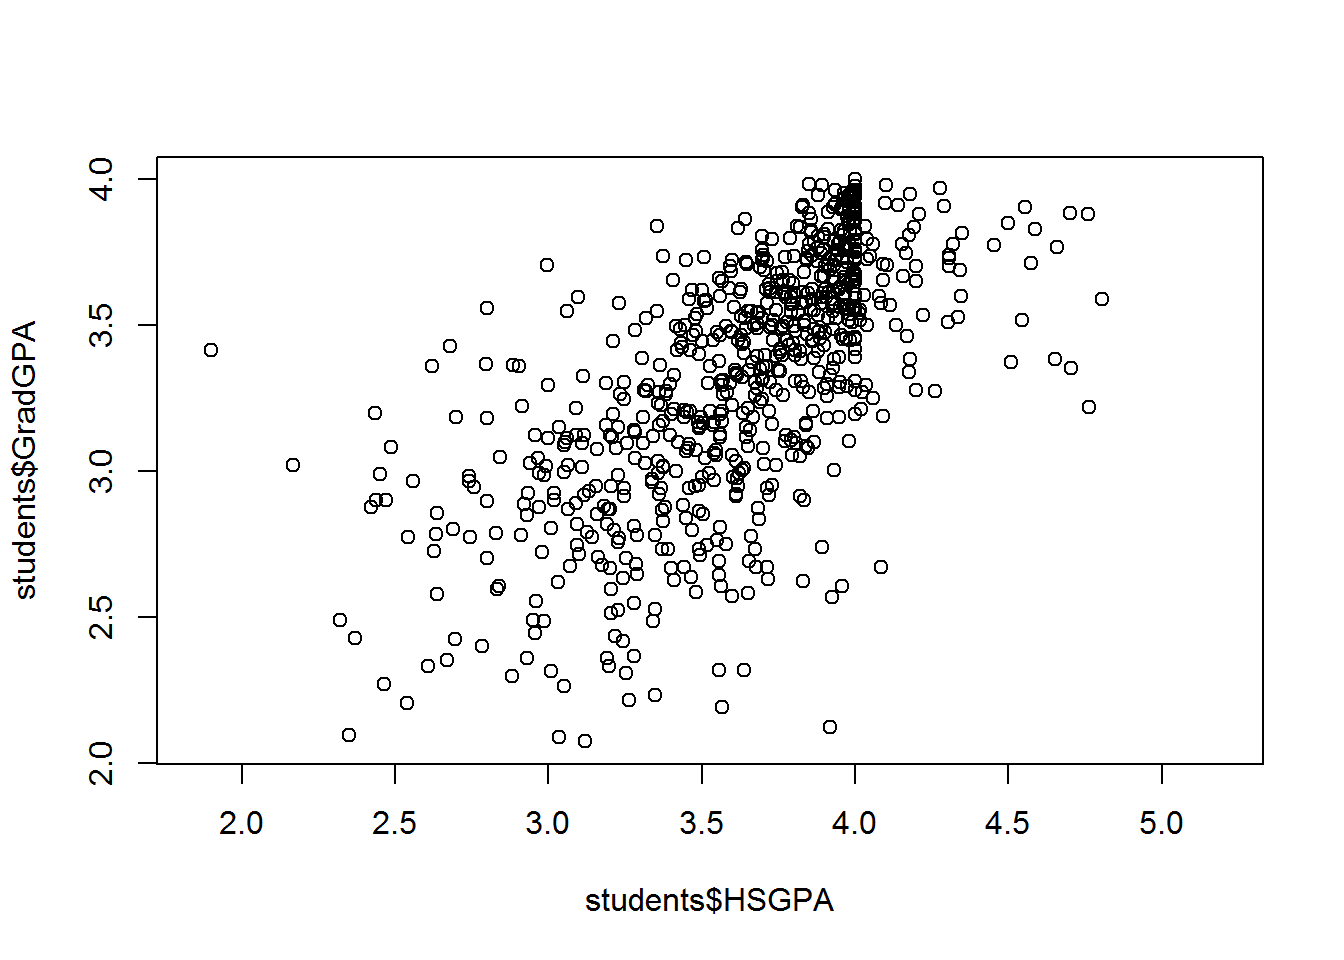
\includegraphics{fastR-Notes_files/figure-latex/unnamed-chunk-50-6.pdf}

Another plotting program that is one of the most popular is ggplot.

\begin{Shaded}
\begin{Highlighting}[]
\KeywordTok{require}\NormalTok{(ggplot2)}
\end{Highlighting}
\end{Shaded}

\begin{Shaded}
\begin{Highlighting}[]
\KeywordTok{qplot}\NormalTok{(HSGPA,GradGPA,}\DataTypeTok{data=}\NormalTok{students)}
\end{Highlighting}
\end{Shaded}

\begin{verbatim}
## Warning: Removed 279 rows containing missing values (geom_point).
\end{verbatim}

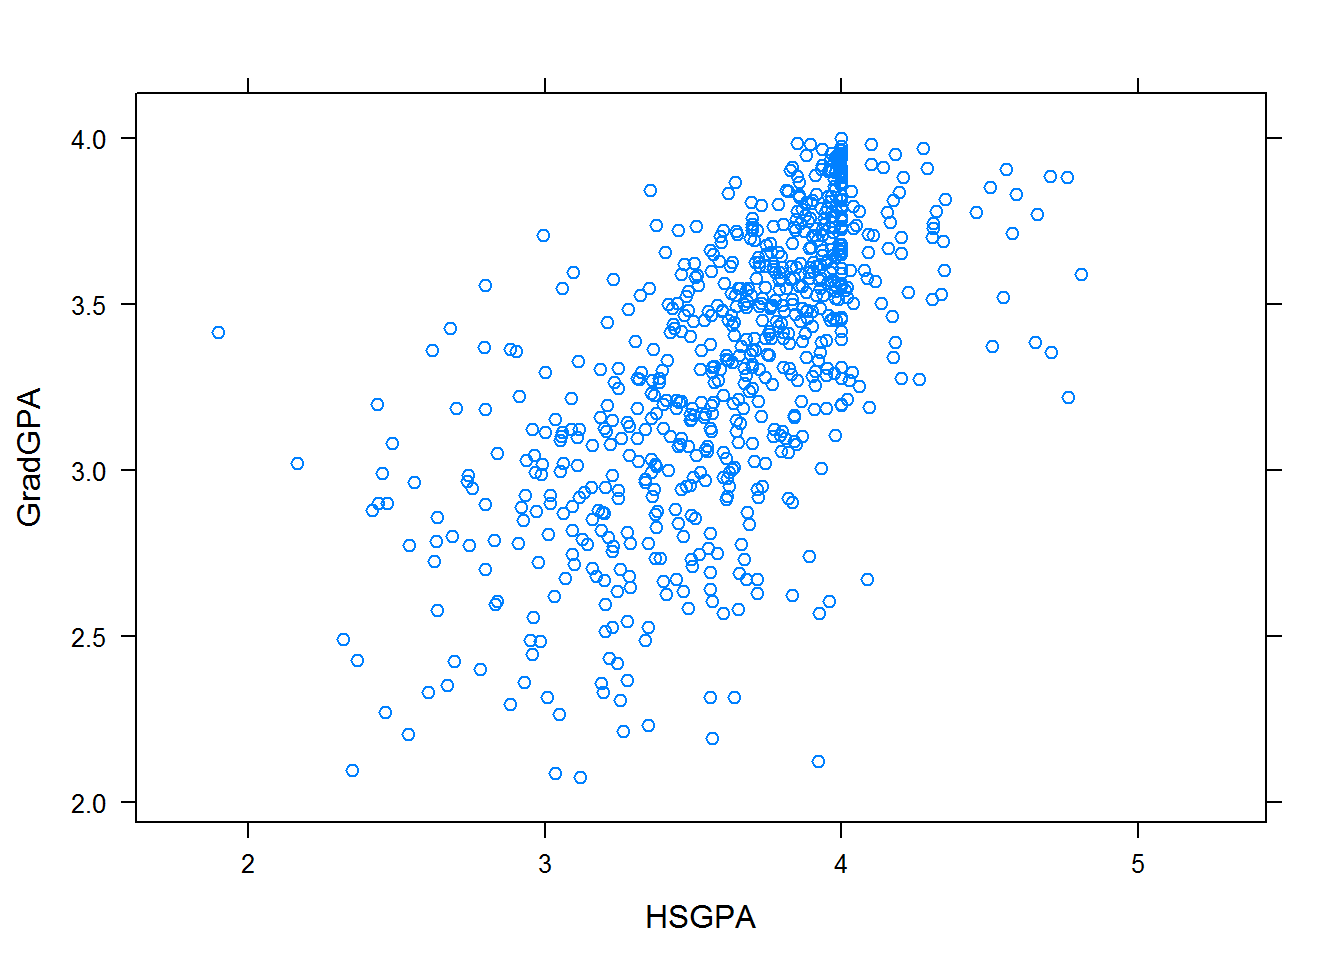
\includegraphics{fastR-Notes_files/figure-latex/unnamed-chunk-52-1.pdf}

The example from the book.

\begin{Shaded}
\begin{Highlighting}[]
\KeywordTok{xtabs}\NormalTok{(}\OperatorTok{~}\NormalTok{Defendant}\OperatorTok{+}\NormalTok{Penalty,deathPenalty)}
\end{Highlighting}
\end{Shaded}

\begin{verbatim}
##          Penalty
## Defendant Death Not
##     Black    17 149
##     White    19 141
\end{verbatim}

\begin{Shaded}
\begin{Highlighting}[]
\KeywordTok{prop.table}\NormalTok{(}\KeywordTok{xtabs}\NormalTok{(}\OperatorTok{~}\NormalTok{Defendant}\OperatorTok{+}\NormalTok{Penalty,deathPenalty),}\DecValTok{2}\NormalTok{)}
\end{Highlighting}
\end{Shaded}

\begin{verbatim}
##          Penalty
## Defendant     Death       Not
##     Black 0.4722222 0.5137931
##     White 0.5277778 0.4862069
\end{verbatim}

\begin{Shaded}
\begin{Highlighting}[]
\KeywordTok{xtabs}\NormalTok{(}\OperatorTok{~}\NormalTok{Defendant}\OperatorTok{+}\NormalTok{Victim}\OperatorTok{+}\NormalTok{Penalty,deathPenalty)}
\end{Highlighting}
\end{Shaded}

\begin{verbatim}
## , , Penalty = Death
## 
##          Victim
## Defendant Black White
##     Black     6    11
##     White     0    19
## 
## , , Penalty = Not
## 
##          Victim
## Defendant Black White
##     Black    97    52
##     White     9   132
\end{verbatim}

\chapter{Probability and Random Variables}\label{Chpt2}

The second chapter is completed in eight lessons. Section 2.2 of the
book has been historically difficult for the students so I have broken
it into two lessons. Also in the first lesson, I have added material
from section B of the book as some students are deficient in this
knowledge.

\hypertarget{L4}{\section{Random Variables}\label{L4}}

\subsection{Objectives}\label{objectives-3}

\begin{enumerate}
\def\labelenumi{\arabic{enumi}.}
\tightlist
\item
  Know definitions introduced in the section, of particular importance
  is Random Variable
\item
  Use set notation
\end{enumerate}

\subsection{Teminology}\label{teminology}

Probability and randomness are difficult and deep philosophical
questions. We will make it easier by looking at repeatable random
process. A process has to have more than one possible outcome.

Some new terms

Outcome\\
Event\\
Sample space Probability\\
Random Variable

If set notation is new, read Appendix B.

We can have deductive probabilities, mostly what we do in this class,
and inductive empirical probabilities.

Do Problem 2.1

Do Problem B-1

Summation and product notation is difficult

Do 1.10

\section{Probability Rules}\label{L5}

\subsection{Objectives}\label{objectives-4}

\begin{enumerate}
\def\labelenumi{\arabic{enumi}.}
\tightlist
\item
  Solve counting problems using bijection, multiplication, complement,
  division, and inclusion-exclusion rules\\
\item
  Use proper notation\\
\item
  Find probabilities using counting rules
\end{enumerate}

\subsection{Probability: General}\label{probability-general}

We will be using the deductive notion of probability, theoretical
probability, in this section. That is, we make use of the axioms on page
31 and results derived from them.

Technically, probability is a space, but we will make it easier by
thinking of it as a function from the sample space to a real number in
\([0,1]\). Often the sample space is a random variable.

The big issue for students when first working with probability is
confusing the algebra of sets with the algebra of numbers. So the
following are all valid for some event \(E\):

\[ E \cup E^c  \] \[P(E \cup E^c)\] \[P(E)+P(E^c)=1\]

So from the axioms, we get: \[E \cup E^c = S \] \[P(E \cup E^c)=P(S)\]
because \(E\) and \(E^c\) are mutually exclusive: \[P(E)+P(E^c)=1\]
\[P(E)=1-P(E^c)\]

Notice that the following are nonsensical: \[P(E) \cup P(E^c)\]
\[E + E^c\]

\subsection{Counting}\label{counting}

We will be making indirect use of the bijection principle as we are
always mapping from objects to numbers. In addition, in using counting,
we are making use of the equally likely rule. This is an assumption and
we must always be aware of the assumptions and whether they apply.

In our counting problems we have to determine if we are sampling with
replacement or not and whether order matters or not. Determining if
order matters is difficult and takes practice. To set up these four
possibilities we will use a simple case of 3 balls and 10 people, this
is an example from the book. All of these methods make use of the
multiplication principle.

\textbf{Problem 1:} We have three different colored balls that we will
give to 10 people. A person can get more than one ball. How many ways
can we distribute the balls?

We can think of the ten people as the numbers, this is the bijection
rule. Since each person can get more than one ball, we are sampling with
replacement. Since the balls are different colors, then order matters.
For example, if Billy gets the blue and green ball, and Sally gets the
red ball. This is different from Billy getting the red and blue, and
Sally getting the green. To solve this problem, we use the
multiplication rule. There are 10 choices of people to give the first
ball to. There are 10 for the second ball and 10 for the third. Thus
there are \(10^3\) or \(1000\) ways.

\textbf{Problem 2:} Same problem but now each person can get at most one
ball. In this case order matters but we sample without replacement. Thus
we have 10 choices for the first ball, 9 for the second, and 8 for the
third. This is called a permutation. Let's write our own function for
this.

\begin{Shaded}
\begin{Highlighting}[]
\NormalTok{perm<-}\ControlFlowTok{function}\NormalTok{(n,r)\{}
\NormalTok{    result<-}\KeywordTok{prod}\NormalTok{(n}\OperatorTok{:}\NormalTok{(n}\OperatorTok{-}\NormalTok{r}\OperatorTok{+}\DecValTok{1}\NormalTok{))}
    \KeywordTok{return}\NormalTok{(result)}
\NormalTok{\}}
\end{Highlighting}
\end{Shaded}

For our problem

\begin{Shaded}
\begin{Highlighting}[]
\KeywordTok{perm}\NormalTok{(}\DecValTok{10}\NormalTok{,}\DecValTok{3}\NormalTok{)}
\end{Highlighting}
\end{Shaded}

\begin{verbatim}
## [1] 720
\end{verbatim}

The notation for a permutation is \(_{n}P_{k}\) and the formula is
\[{n! \over (n-k)!}\]

Note that we must define 0!=1 to make this work.

\textbf{Problem 3:} Let's do problem 2 but this time the balls are all
the same color. In this case the order does not matter. To understand
what to do, make the problem simpler and enumerate. Let's say we have
three people \{Billy, Sally, Tommy\} and two red balls. If ordered
mattered we could enumerate the permutations using tuples. The first
position represents ball 1 and the second ball 2. Thus we have 6
possibilities:

\begin{Shaded}
\begin{Highlighting}[]
\KeywordTok{perm}\NormalTok{(}\DecValTok{3}\NormalTok{,}\DecValTok{2}\NormalTok{)}
\end{Highlighting}
\end{Shaded}

\begin{verbatim}
## [1] 6
\end{verbatim}

(Billy, Sally), (Billy, Tommy), (Sally, Tommy), (Sally, Billy), (Tommy,
Sally), (Tommy, Billy).

But since the balls are identical (Billy, Sally) is the same as (Sally,
Billy). So we need the division rule to remove redundant outcomes. Each
outcome has two possibilities thus we have 2! ways that are equivalent.
This is a combination and has the notation \(_{n}C_{k}\) and the
formulas:
\[\left( {\begin{array}{c}n \\ k \end{array}} \right) = {n! \over (n-k)!k!}\]
which is the permutation divided by \(k!\).

R has the function \texttt{choose} to find the values for us.

\begin{Shaded}
\begin{Highlighting}[]
\KeywordTok{choose}\NormalTok{(}\DecValTok{10}\NormalTok{,}\DecValTok{3}\NormalTok{)}
\end{Highlighting}
\end{Shaded}

\begin{verbatim}
## [1] 120
\end{verbatim}

\textbf{Problem 4:} Now this is a difficult one and that is when order
does not matter and we sample with replacement. This is the most
difficult and is what is being done in Example 2.2.14 in the book. Let's
look at the simple case of three people and two identical balls. We have
the following results (Billy, Billy), (Billy, Sally), (Billy, Tommy),
(Sally, Sally), (Sally, Tommy), and (Tommy, Tommy). There are six ways
to do this. This is equivalent to solving the problem of finding the
number of solutions to \[x_1 + x_2 + x_3 =3\] Where \(x_1\) is the
number of balls Billy is given, etc. This is the bijection rule.

This problem is solved by thinking of vertical lines representing the
numbers of balls someone is given and the plus signs between the
vertical lines. Thus one outcome is Billy receives all three balls. This
would be \textbar{}\textbar{}\textbar{}++. If each person were given a
ball, this would look like \textbar{}+\textbar{}+\textbar{}. Thus we
have \(k\) vertical lines and \(n-1\) plus signs. Using this bijection,
the number of solutions is

\[\left( {\begin{array}{c}n+k-1 \\ k \end{array}} \right) = {(n+k-1)! \over (n-1)!k!}\]

For the problem with 3 people and 2 identical balls.

\begin{Shaded}
\begin{Highlighting}[]
\KeywordTok{choose}\NormalTok{((}\DecValTok{3}\OperatorTok{+}\DecValTok{2}\OperatorTok{-}\DecValTok{1}\NormalTok{),}\DecValTok{2}\NormalTok{)}
\end{Highlighting}
\end{Shaded}

\begin{verbatim}
## [1] 6
\end{verbatim}

And for the problem with 10 people and 3 identical balls.

\begin{Shaded}
\begin{Highlighting}[]
\KeywordTok{choose}\NormalTok{((}\DecValTok{10}\OperatorTok{+}\DecValTok{3}\OperatorTok{-}\DecValTok{1}\NormalTok{),}\DecValTok{3}\NormalTok{)}
\end{Highlighting}
\end{Shaded}

\begin{verbatim}
## [1] 220
\end{verbatim}

We can combine these ideas with the multiplication rule. The question of
order is the most difficult part. For example, if we roll two dice and
record the values on the faces, how many possibilities are there?

\subsection{Probability: Equally Likely
Events}\label{probability-equally-likely-events}

For equally likely events, we find the probability by dividing the
number of ways of the event by the number of ways in the sample space.

Drawing five cards from a deck of cards, what is the probability that at
least two cards have the same face value?

The denominator is \(_{52}C_{5}\)

\begin{Shaded}
\begin{Highlighting}[]
\KeywordTok{choose}\NormalTok{(}\DecValTok{52}\NormalTok{,}\DecValTok{5}\NormalTok{)}
\end{Highlighting}
\end{Shaded}

\begin{verbatim}
## [1] 2598960
\end{verbatim}

For the numerator we will use the complement rule. Thus we need to
select 5 face card values of different values. We select 5 face card
values from 13 without replacement. Order does not matter. Then for each
face value we have 4 suits. Thus the numerator is:

\begin{Shaded}
\begin{Highlighting}[]
\KeywordTok{choose}\NormalTok{(}\DecValTok{13}\NormalTok{,}\DecValTok{5}\NormalTok{)}\OperatorTok{*}\DecValTok{4}\OperatorTok{^}\DecValTok{5}
\end{Highlighting}
\end{Shaded}

\begin{verbatim}
## [1] 1317888
\end{verbatim}

By the division rule, we have the probability as

\begin{Shaded}
\begin{Highlighting}[]
\NormalTok{(}\KeywordTok{choose}\NormalTok{(}\DecValTok{13}\NormalTok{,}\DecValTok{5}\NormalTok{)}\OperatorTok{*}\DecValTok{4}\OperatorTok{^}\DecValTok{5}\NormalTok{)}\OperatorTok{/}\KeywordTok{choose}\NormalTok{(}\DecValTok{52}\NormalTok{,}\DecValTok{5}\NormalTok{)}
\end{Highlighting}
\end{Shaded}

\begin{verbatim}
## [1] 0.5070828
\end{verbatim}

And the probability we want is

\begin{Shaded}
\begin{Highlighting}[]
\DecValTok{1}\OperatorTok{-}\NormalTok{(}\KeywordTok{choose}\NormalTok{(}\DecValTok{13}\NormalTok{,}\DecValTok{5}\NormalTok{)}\OperatorTok{*}\DecValTok{4}\OperatorTok{^}\DecValTok{5}\NormalTok{)}\OperatorTok{/}\KeywordTok{choose}\NormalTok{(}\DecValTok{52}\NormalTok{,}\DecValTok{5}\NormalTok{)}
\end{Highlighting}
\end{Shaded}

\begin{verbatim}
## [1] 0.4929172
\end{verbatim}

How about the probability that all the cards come from the same suit, a
flush?

\begin{Shaded}
\begin{Highlighting}[]
\NormalTok{(}\KeywordTok{choose}\NormalTok{(}\DecValTok{13}\NormalTok{,}\DecValTok{5}\NormalTok{)}\OperatorTok{*}\KeywordTok{choose}\NormalTok{(}\DecValTok{4}\NormalTok{,}\DecValTok{1}\NormalTok{))}\OperatorTok{/}\KeywordTok{choose}\NormalTok{(}\DecValTok{52}\NormalTok{,}\DecValTok{5}\NormalTok{)}
\end{Highlighting}
\end{Shaded}

\begin{verbatim}
## [1] 0.001980792
\end{verbatim}

Homework 2.6 and 2.7

Note that \[{_{13}P_{2}}= {_{13}C_{1}} * {_{12}C_{1}}\]

\hypertarget{L6}{\section{Inclusion-Exclusion, Conditional
Probability}\label{L6}}

\subsection{Objectives}\label{objectives-5}

\begin{enumerate}
\def\labelenumi{\arabic{enumi}.}
\tightlist
\item
  Using definitions, calculate conditioning probabilities\\
\item
  Determine if events are independent, or if events are independent find
  joint probabilities\\
\item
  Use Bayes theorem to find conditional probabilities
\end{enumerate}

\subsection{Definitions}\label{definitions}

Know these

\[P(A \cup B)=P(A)+P(B)-P(A \cap B)\] Iff \(A\) and \(B\) are
independent \[P(A \cap B)=P(A)P(B)\] or equivalently \[P(A|B)=P(A)\] If
\(A\) and \(B\) are mutually exclusive \[P(A \cap B)=0\] Finally,
conditional probability which takes practice to master and understand
\[P(A|B)={P(A \cap B) \over P(B)}\]

Other relationships can be derived from drawing Venn diagrams. For
example:
\[P(A)=P((A \cap B) \cup (A \cap B^c))=P(A\cap B) + P(A \cap B^c)\]

Independence is difficult to visualize on a Venn diagram since it is a
ratio of areas and humans do not perceive difference in areas very well.

In many problems we need to find \(P(A \cap B)\). There are many ways to
do this but the most common using conditional probability.
\[P(A \cap B)=P(A|B)P(B)=P(B|A)P(A)\]

Another confusion is with the given part of the conditional probability.
The given event is not random, it did happen. Thus the sample space is
reduced, this is why division by the probability of the given event is
happening. The book does a nice example with Example 2.2.15.

The second most common way to find \(P(A \cap B)\) is with independence
so that \[P(A \cap B)=P(A)P(B)\]

\subsection{Problems}\label{problems}

\begin{enumerate}
\def\labelenumi{\arabic{enumi}.}
\tightlist
\item
  We shuffle a deck of cards and turn the top card over. It is an Ace.
  What is the probability the second card is an Ace?
\end{enumerate}

Let A - face value on first card is an Ace and B - face value on the
second card is an Ace

we want \(P(B|A)\). Given that the first card is an Ace we have 51 cards
left and 3 are Aces.

\begin{enumerate}
\def\labelenumi{\arabic{enumi}.}
\setcounter{enumi}{1}
\tightlist
\item
  We shuffle a deck of cards and turn the top cards over. What is the
  probability we have two Aces?
\end{enumerate}

Let A - face value on first card is an Ace and B - face value on the
second card is an Ace

We want \(P(A \cap B)\). Using conditional probability

\[P(A \cap B) =P(A)P(B|A)={4 \over 52}{3 \over 51}\]

\begin{enumerate}
\def\labelenumi{\arabic{enumi}.}
\setcounter{enumi}{2}
\tightlist
\item
  We shuffle a deck of cards and set the first card to the side without
  revealing it. What is the probability the second card is an Ace?
\end{enumerate}

Intuitively we know the answer is \({4 \over 52}\) but let's use our
probability rules to find it.

Let A - face value on first card is an Ace and B - face value on the
second card is an Ace

We want \(P(B)\)

Now \[P(B)=P(A \cap B)+P(A^c \cap B)\] where now
\[P(A \cap B)=P(B|A)P(A)={4 \over 52}{3 \over 51}\] and
\[P(A^c \cap B)=P(B|A^c)P(A^c)={48 \over 52}{4 \over 51}\] Finally
\[P(B)=P(A \cap B)+P(A^c \cap B)={4 \over 52}{3 \over 51}+{48 \over 52}{4 \over 51}\]
\[={4 \over 52}\left({3 \over 51}+{48 \over 51}\right)={4 \over 52}\]

\begin{enumerate}
\def\labelenumi{\arabic{enumi}.}
\setcounter{enumi}{3}
\tightlist
\item
  We shuffle a deck of cards and set the first card to the side without
  revealing it. The second card is an Ace, what is the probability the
  first card is an Ace?
\end{enumerate}

Let A - face value on first card is an Ace and B - face value on the
second card is an Ace

We want \(P(A|B)\)

From the definition of conditional probability, we have

\[P(A|B)={P(A \cap B) \over P(B)}={P(B|A)P(A) \over P(B)}={P(B|A)P(A) \over P(A \cap B)+P(A^c \cap B)}={P(B|A)P(A) \over P(B|A)P(A)+P(B|A^c)P(A^c)}\]

This is Bayes Rule and comes from the definition of conditional
probability.

The answer is
\[P(A|B)={{4 \over 52}{3 \over 51} \over {4 \over 52}{3 \over 51}+ {48 \over 52}{4 \over 51}}\]
\[={{3 \over 51} \over {3 \over 51}+ {48 \over 51}}={3 \over 51}\]

\subsection{Bayes Rule}\label{bayes-rule}

From Example 2.2.22:

\emph{Suppose a test correctly identifies diseased people 98\% of the
time and correctly identifies healthy people 99\% of the time.
Furthermore assume that in a certain population, one person in 1000 has
the disease. If a random person is tested and the test comes back
positive, what is the probability that the person has the disease?}

This problem can be done as a tree and many of you may have seen this
approach. However, we will use numbers instead of proportions. It is
more difficult for us to understand and interpret proportions as
compared to numbers. Let's proceed using numbers.

Suppose we have 100,000 people. 100 will be diseased and 99900 will be
healthy. Of those that are diseased, 2 will test negative and 98
positive. Of those that are healthy, 999 will test positive and 97902
will test negative. Now of those that test positive, how many will be
diseased? \[P(D|+)={98 \over 98+999}=0.08933455\]

Practice Exam Question

My birthday is March 26, what is the probability at least one of my 23
students in class will have the same birthday?

\hypertarget{L7}{\section{Discrete Distributions}\label{L7}}

\subsection{Objectives}\label{objectives-6}

\begin{enumerate}
\def\labelenumi{\arabic{enumi}.}
\tightlist
\item
  Use, including proper notations, terms and definitions such as
  probability mass function, cumulative distribution functions, etc.\\
\item
  Solve probability problems, including the use of R, for binomial and
  negative binomial random variables.\\
\item
  Explain the assumptions of the binomial and negative binomial
  distributions.
\end{enumerate}

\subsection{Definitions}\label{definitions-1}

Again, you must learn and know the definitions in this section. The pmf
and cdf are confusing to students when first learning but think of the
pmf as a function that maps from the random variable to a probability.
We know that probabilities have to be in \([0,1]\) and the sum of all
the probabilities must be 1.

The cdf, cumulative distribution function is simply \(P(X \leq x)\). The
capital notation is for a random variable and the lower for a value of
the random variable.

\subsection{Practice}\label{practice}

You flip a coin two times where the probability of heads is 0.51.

\begin{enumerate}
\def\labelenumi{\arabic{enumi}.}
\tightlist
\item
  Write the sample space\\
\item
  Create a random variable for this scenario\\
\item
  Write the probability mass function
\item
  Write the cdf\\
\item
  Use R to find\\
\end{enumerate}

\begin{enumerate}
\def\labelenumi{\roman{enumi}.}
\tightlist
\item
  \(P(X=2)\)\\
\item
  \(P(X=0 \cup X=2)\)\\
\end{enumerate}

\begin{enumerate}
\def\labelenumi{\arabic{enumi}.}
\setcounter{enumi}{5}
\tightlist
\item
  Is this a binomial?
\end{enumerate}

Do Problem 2.43

\hypertarget{L8}{\section{Introduction to Hypothesis Testing}\label{L8}}

\subsection{Objectives}\label{objectives-7}

\begin{enumerate}
\def\labelenumi{\arabic{enumi}.}
\tightlist
\item
  Correctly use all new terminology and definitions to include:
  statistic, test statistic, p-value, Type I error, Type II error,
  power, null hypothesis, and alternative hypothesis\\
\item
  Conduct a statistical hypothesis test using the four steps introduced
  in the book\\
\item
  Conduct a power analysis
\end{enumerate}

\subsection{Hypotheses Testing}\label{hypotheses-testing}

Hypothesis testing is difficult to understand and requires thought and
practice. The examples in the book are good and detailed. I am going to
simplify the example here to help learn the definitions, but you must
then wrestle with the examples in the book. I am going to use a simple
hypothesis where as the book is using a complex.

I am going to generate a random sample from a binomial where the number
of trials is 100. The probability of success is either .45 or .5 and
your job is empirically test which value you think I used based on the
data. First let's practice the command \texttt{rbinom}. To get sample I
could do the following commands, I set the seed to make sure I can
repeat the results.

\begin{Shaded}
\begin{Highlighting}[]
\NormalTok{(temp<-}\KeywordTok{rbinom}\NormalTok{(}\DecValTok{100}\NormalTok{,}\DecValTok{1}\NormalTok{,.}\DecValTok{45}\NormalTok{))}
\end{Highlighting}
\end{Shaded}

\begin{verbatim}
##   [1] 0 0 0 0 0 0 1 0 1 0 0 1 1 1 1 1 0 1 1 1 0 1 0 0 1 0 0 1 1 0 0 1 0 0 0
##  [36] 1 0 0 1 0 1 1 1 1 1 0 1 0 0 1 0 0 0 1 1 1 0 1 0 0 0 0 1 0 0 0 1 1 0 0
##  [71] 0 0 1 0 0 0 1 0 0 0 0 1 0 0 0 1 1 0 0 0 1 0 0 1 0 1 0 0 1 1
\end{verbatim}

\begin{Shaded}
\begin{Highlighting}[]
\KeywordTok{sum}\NormalTok{(temp)}
\end{Highlighting}
\end{Shaded}

\begin{verbatim}
## [1] 41
\end{verbatim}

Note: A success is a 1 and a failure is a 0.

Thus in this random process, I had 41 successes out of 100 trials. This
is a binomial because each trial is independent, the probability of
success is constant, the trial are fixed, and each trial has two
outcomes.

I could have also done

\begin{Shaded}
\begin{Highlighting}[]
\KeywordTok{rbinom}\NormalTok{(}\DecValTok{1}\NormalTok{,}\DecValTok{100}\NormalTok{,.}\DecValTok{45}\NormalTok{)}
\end{Highlighting}
\end{Shaded}

\begin{verbatim}
## [1] 38
\end{verbatim}

For interest what would \texttt{rbinom(10,100,.45)} give you?

I will generate a sample with the probability of success as either .45
or .50. You must decide which you think it is.

\subsubsection{Step 1: State the null and alternative
hypotheses}\label{step-1-state-the-null-and-alternative-hypotheses}

State the null and alternative hypothesis. In practice, the alternative
is set to the condition that you want to demonstrate. This is similar to
a criminal trial where you are the prosecutor and you want to show that
the accused is guilty. The null is that the accused is innocent and the
alternative is that they are guilty.

For this artificial problem, it is not clear what the alternative should
be. Thus we will select the alternative as the probability of success is
0.5. The hypotheses are:

\[H_{o}: \pi = 0.45 \] \[H_{a}: \pi = 0.50 \]

Here \(\pi\) is the unknown population parameter probability of success.

\subsubsection{Step 2: Calculate a test
statistic}\label{step-2-calculate-a-test-statistic}

We run 100 trials and get

\begin{verbatim}
## [1] 49
\end{verbatim}

successes.

The estimate of the probability of success \texttt{49/100} or
\texttt{0.49}. We will learn more about these types of estimates. They
are called point estimates.

We could have many different test statistics and the choice is important
for analysis. We will discuss properties later in the course. But two
examples of test statistics are the proportion of success \texttt{0.49}
and the number of success \texttt{49}. We will use the number of
successes. The statistic is the number of successes, a random variable,
and the test statistic is 49.

\subsubsection{Step 3: Compute the
p-value}\label{step-3-compute-the-p-value}

The definition of p-value is a conditional probability. Given that null
hypothesis is true, what is the probability of the data or more extreme.
The difficult part is what is meant by more extreme. Our statistic is
the number of successes out of 100 trials. It is a binomial.

Before we calculate the p-value, let's think about how we could decide
whether we believe that the data comes with the probability of success
equal to \texttt{.45} or \texttt{0.50}. It seems that since \texttt{.49}
is closer that we think it should be \texttt{0.50}. Let's plot the
probability mass function for each case.

\begin{Shaded}
\begin{Highlighting}[]
\KeywordTok{plot}\NormalTok{((}\DecValTok{30}\OperatorTok{:}\DecValTok{70}\NormalTok{),}\KeywordTok{dbinom}\NormalTok{((}\DecValTok{30}\OperatorTok{:}\DecValTok{70}\NormalTok{),}\DecValTok{100}\NormalTok{,.}\DecValTok{45}\NormalTok{),}\DataTypeTok{type=}\StringTok{"p"}\NormalTok{,}\DataTypeTok{xlab=}\StringTok{"Number of Successes"}\NormalTok{,}\DataTypeTok{ylab=}\StringTok{"Probability"}\NormalTok{)}
\KeywordTok{points}\NormalTok{((}\DecValTok{30}\OperatorTok{:}\DecValTok{70}\NormalTok{),}\KeywordTok{dbinom}\NormalTok{((}\DecValTok{30}\OperatorTok{:}\DecValTok{70}\NormalTok{),}\DecValTok{100}\NormalTok{,.}\DecValTok{5}\NormalTok{),}\DataTypeTok{type=}\StringTok{"p"}\NormalTok{,}\DataTypeTok{col=}\DecValTok{2}\NormalTok{)}
\KeywordTok{abline}\NormalTok{(}\DataTypeTok{v=}\DecValTok{49}\NormalTok{)}
\end{Highlighting}
\end{Shaded}

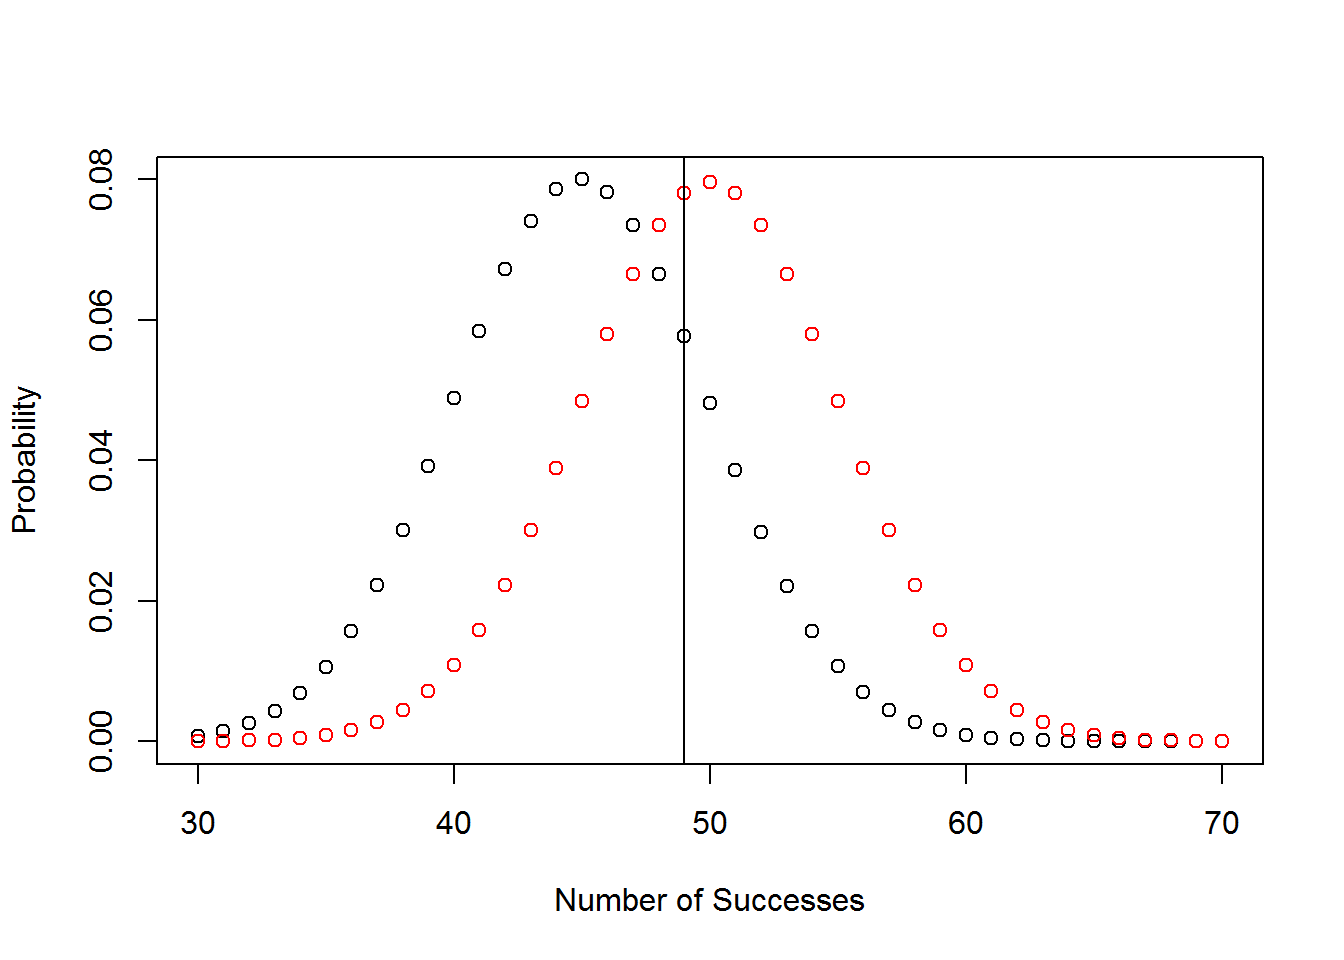
\includegraphics{fastR-Notes_files/figure-latex/unnamed-chunk-70-1.pdf}

Notice the use of \texttt{dbinom} in this code.

One way to decide is to pick a rejection region where the probability of
that number of successes is higher under each different value of the
probability of success. We can find these by creating a table.

\begin{Shaded}
\begin{Highlighting}[]
\NormalTok{prob_table<-}\KeywordTok{rbind}\NormalTok{(}\KeywordTok{dbinom}\NormalTok{((}\DecValTok{40}\OperatorTok{:}\DecValTok{60}\NormalTok{),}\DecValTok{100}\NormalTok{,.}\DecValTok{45}\NormalTok{),}\KeywordTok{dbinom}\NormalTok{((}\DecValTok{40}\OperatorTok{:}\DecValTok{60}\NormalTok{),}\DecValTok{100}\NormalTok{,.}\DecValTok{5}\NormalTok{))}
\KeywordTok{colnames}\NormalTok{(prob_table)<-(}\DecValTok{40}\OperatorTok{:}\DecValTok{60}\NormalTok{)}
\KeywordTok{row.names}\NormalTok{(prob_table)<-}\KeywordTok{c}\NormalTok{(}\StringTok{"Prob = 0.45"}\NormalTok{,}\StringTok{"Prob = 0.50"}\NormalTok{)}
\NormalTok{prob_table}
\end{Highlighting}
\end{Shaded}

\begin{verbatim}
##                     40         41         42         43         44
## Prob = 0.45 0.04880290 0.05843363 0.06716073 0.07411819 0.07855915
## Prob = 0.50 0.01084387 0.01586907 0.02229227 0.03006864 0.03895256
##                    45         46         47         48         49
## Prob = 0.45 0.0799875 0.07824864 0.07355675 0.06645184 0.05769844
## Prob = 0.50 0.0484743 0.05795840 0.06659050 0.07352701 0.07802866
##                     50         51         52         53         54
## Prob = 0.45 0.04815197 0.03862458 0.02977874 0.02206589 0.01571359
## Prob = 0.50 0.07958924 0.07802866 0.07352701 0.06659050 0.05795840
##                     55          56          57          58          59
## Prob = 0.45 0.01075277 0.007069597 0.004465009 0.002708399 0.001577465
## Prob = 0.50 0.04847430 0.038952560 0.030068643 0.022292270 0.015869073
##                       60
## Prob = 0.45 0.0008819463
## Prob = 0.50 0.0108438667
\end{verbatim}

Based on this table, if we have 47 or less successes, we should fail to
reject that \(\pi = 0.45\) while 48 or more means we reject \(H_{o}\) in
favor of \(H_{a}\). We use the fail to reject instead of accept just
like we use not guilty instead of innocent. This idea of finding a
cutpoint number is called the rejection region. Using the test statistic
of \texttt{49}, which is greater than \texttt{47}, we would reject
\(H_{o}: \pi = 0.45\) in favor of \(H_{a}: \pi = 0.50\).

Another, and more common, method to determine the rejection region is to
find the quantile associated with a small probability. This probability
is called the significance level and is usually set to \texttt{0.05}. It
turns out it is the probability of rejecting when the null is true. In
this case we want to find the number of successes such that having that
value or more extreme leads to a probability of 0.05. Why 0.05? This is
unusual enough that we think that if it happens we conclude the null is
not true. It is a sort of empirical proof by contradiction. Since we
will reject \(H_{o}: \pi = 0.45\) in favor of \(H_{a}: \pi = 0.50\) only
if the number of success is larger than the rejection value, we want the
0.05 probability to be in the upper tail. Thus we can use
\texttt{qbinom}.

\begin{Shaded}
\begin{Highlighting}[]
\KeywordTok{qbinom}\NormalTok{(.}\DecValTok{95}\NormalTok{,}\DecValTok{100}\NormalTok{,.}\DecValTok{45}\NormalTok{)}
\end{Highlighting}
\end{Shaded}

\begin{verbatim}
## [1] 53
\end{verbatim}

Just to check

\begin{Shaded}
\begin{Highlighting}[]
\DecValTok{1}\OperatorTok{-}\KeywordTok{pbinom}\NormalTok{(}\DecValTok{52}\OperatorTok{:}\DecValTok{53}\NormalTok{,}\DecValTok{100}\NormalTok{,.}\DecValTok{45}\NormalTok{)}
\end{Highlighting}
\end{Shaded}

\begin{verbatim}
## [1] 0.06617290 0.04410701
\end{verbatim}

Since the distribution is discrete, we cannot find a quantile that will
give us exactly 0.05 in the upper tail. We have a choice. If we reject
when the number of successes is 53 or greater then percentile is 0.066.
Likewise if we use 54 or greater, then the percentile is 0.044. I will
go with the second because it is conservative. This choice has to do
with a Type I error, which we will discuss shortly.

Based on this rejection region and the data, we fail to reject
\(H_{o}: \pi = 0.45\) in favor of \(H_{a}: \pi = 0.50\).

The p-value is a similar idea but takes the context of the problem out
of the decision. Under the null hypothesis, the probability of success
is \texttt{0.45}. To find the p-value, we calculate the probability of
the data or more extreme under the null hypothesis. More extreme means
further from the null and more towards the alternative. Thus for us we
want to find \(P(X \geq 49)\) which using R is

\begin{Shaded}
\begin{Highlighting}[]
\DecValTok{1}\OperatorTok{-}\KeywordTok{pbinom}\NormalTok{(}\DecValTok{48}\NormalTok{,}\DecValTok{100}\NormalTok{,.}\DecValTok{45}\NormalTok{)}
\end{Highlighting}
\end{Shaded}

\begin{verbatim}
## [1] 0.2404266
\end{verbatim}

\begin{Shaded}
\begin{Highlighting}[]
\KeywordTok{pbinom}\NormalTok{(}\DecValTok{48}\NormalTok{,}\DecValTok{100}\NormalTok{,.}\DecValTok{45}\NormalTok{,}\DataTypeTok{lower=}\OtherTok{FALSE}\NormalTok{)}
\end{Highlighting}
\end{Shaded}

\begin{verbatim}
## [1] 0.2404266
\end{verbatim}

Since this is larger than our significance level of 0.05, we fail to
reject \(H_{o}: \pi = 0.45\) in favor of \(H_{a}: \pi = 0.50\).

Which test is better, one rejected and the other did not? It is beyond
the scope of this course, but is based on the idea of finding uniformly
most powerful tests.

\subsubsection{Draw a conclusion}\label{draw-a-conclusion}

Based on our data of 49 successes in 100 tries, under the null that the
probability of heads is \texttt{0.45} we found the probability of 49 or
more heads is 0.2404 which is greater than 0.05. Thus we fail to reject
\(H_{o}: \pi = 0.45\) in favor of \(H_{a}: \pi = 0.50\).

\subsection{More terms - Errors}\label{more-terms---errors}

We can make two types of error. We can reject when the null is true.
This is a type I error. The probability of this is the significance
level, usually called \(\alpha\). Formally, the probability of a type I
error is \texttt{P(reject\textbar{}null\ hypothesis\ is\ true)}. We pick
this value as part of the test design. This is why we put what we are
trying to show in the alternative because we are trying to reject the
null and we can control the type I error.

The second type of error is called the type II error, yes these are poor
names. Sometimes type I error is called a false positive, and type II a
false negative. The type II error is when we fail to reject but the
alternative is true. In practice this is difficult to calculate because
the alternative is often a complex hypothesis and we don't have a value
for the parameter under the alternative. But because I chose a simple
alternative, we can easily find the probability of a type II error. The
probability of a type II error is
\texttt{P(Fail\ to\ reject\textbar{}Alternative\ hypothesis\ is\ true)}.
Based on the work we did above, we reject when the number of successes
is 54 or greater. The probability of a type II error thus is

\begin{Shaded}
\begin{Highlighting}[]
\KeywordTok{pbinom}\NormalTok{(}\DecValTok{53}\NormalTok{,}\DecValTok{100}\NormalTok{,.}\DecValTok{5}\NormalTok{)}
\end{Highlighting}
\end{Shaded}

\begin{verbatim}
## [1] 0.7579408
\end{verbatim}

For our problem, since we failed to reject, the probability of a type II
error is large. Typically we want it at \texttt{0.2} or smaller. For
this problem that means a larger sample size is required. The
calculation of sample size should have been done prior to the test.

The complement of a type II error is called power and it is the
probability we reject given the alternative is true. Again, since we are
setting up in the hopes of rejecting, power is a useful metric. For this
problem, power is

\begin{Shaded}
\begin{Highlighting}[]
\DecValTok{1}\OperatorTok{-}\KeywordTok{pbinom}\NormalTok{(}\DecValTok{53}\NormalTok{,}\DecValTok{100}\NormalTok{,.}\DecValTok{5}\NormalTok{)}
\end{Highlighting}
\end{Shaded}

\begin{verbatim}
## [1] 0.2420592
\end{verbatim}

\subsection{Sample Size}\label{sample-size}

Instead of 100 trials how many should we have done? Using an \(\alpha\)
of 0.05, this is my type II error and a power of at least 0.80. Let's
find the number. As a start, say the sample size is 200. Then the
rejection region is

\begin{Shaded}
\begin{Highlighting}[]
\KeywordTok{qbinom}\NormalTok{(.}\DecValTok{95}\NormalTok{,}\DecValTok{200}\NormalTok{,.}\DecValTok{45}\NormalTok{)}
\end{Highlighting}
\end{Shaded}

\begin{verbatim}
## [1] 102
\end{verbatim}

And the power is

\begin{Shaded}
\begin{Highlighting}[]
\DecValTok{1}\OperatorTok{-}\KeywordTok{pbinom}\NormalTok{(}\DecValTok{102}\NormalTok{,}\DecValTok{200}\NormalTok{,.}\DecValTok{5}\NormalTok{)}
\end{Highlighting}
\end{Shaded}

\begin{verbatim}
## [1] 0.3618855
\end{verbatim}

We are going to need a large sample. Next let's try 800 trials.

\begin{Shaded}
\begin{Highlighting}[]
\KeywordTok{qbinom}\NormalTok{(.}\DecValTok{95}\NormalTok{,}\DecValTok{800}\NormalTok{,.}\DecValTok{45}\NormalTok{)}
\end{Highlighting}
\end{Shaded}

\begin{verbatim}
## [1] 383
\end{verbatim}

And the power is

\begin{Shaded}
\begin{Highlighting}[]
\DecValTok{1}\OperatorTok{-}\KeywordTok{pbinom}\NormalTok{(}\DecValTok{383}\NormalTok{,}\DecValTok{800}\NormalTok{,.}\DecValTok{5}\NormalTok{)}
\end{Highlighting}
\end{Shaded}

\begin{verbatim}
## [1] 0.8783484
\end{verbatim}

That is more like it. I think we can write a function to help us.

\begin{Shaded}
\begin{Highlighting}[]
\NormalTok{simple_sample_size<-}\ControlFlowTok{function}\NormalTok{(}\DataTypeTok{n=}\DecValTok{100}\NormalTok{)\{}\DecValTok{1}\OperatorTok{-}\KeywordTok{pbinom}\NormalTok{(}\KeywordTok{qbinom}\NormalTok{(.}\DecValTok{95}\NormalTok{,n,.}\DecValTok{45}\NormalTok{),n,.}\DecValTok{5}\NormalTok{)\}}
\end{Highlighting}
\end{Shaded}

Now for a range of values

\begin{Shaded}
\begin{Highlighting}[]
\NormalTok{temp<-}\KeywordTok{sapply}\NormalTok{((}\DecValTok{600}\OperatorTok{:}\DecValTok{625}\NormalTok{),simple_sample_size)}
\KeywordTok{names}\NormalTok{(temp)<-(}\DecValTok{600}\OperatorTok{:}\DecValTok{625}\NormalTok{)}
\NormalTok{temp    }
\end{Highlighting}
\end{Shaded}

\begin{verbatim}
##       600       601       602       603       604       605       606 
## 0.7810158 0.7685830 0.7806348 0.7922992 0.7802553 0.7919132 0.7798774 
##       607       608       609       610       611       612       613 
## 0.7915286 0.7795009 0.7911456 0.7791259 0.7907640 0.7787524 0.7903839 
##       614       615       616       617       618       619       620 
## 0.7783803 0.7900052 0.7780097 0.7896280 0.8008639 0.7892522 0.8004829 
##       621       622       623       624       625 
## 0.7888779 0.8001033 0.7885049 0.7997251 0.7881334
\end{verbatim}

So it looks like around 618 trials would work for use. Let's plot

\begin{Shaded}
\begin{Highlighting}[]
\KeywordTok{plot}\NormalTok{((}\DecValTok{249}\OperatorTok{:}\DecValTok{329}\NormalTok{),}\KeywordTok{dbinom}\NormalTok{((}\DecValTok{249}\OperatorTok{:}\DecValTok{329}\NormalTok{),}\DecValTok{618}\NormalTok{,.}\DecValTok{45}\NormalTok{),}\DataTypeTok{type=}\StringTok{"p"}\NormalTok{,}\DataTypeTok{xlab=}\StringTok{"Number of Successes"}\NormalTok{,}\DataTypeTok{ylab=}\StringTok{"Probability"}\NormalTok{)}
\KeywordTok{points}\NormalTok{((}\DecValTok{249}\OperatorTok{:}\DecValTok{329}\NormalTok{),}\KeywordTok{dbinom}\NormalTok{((}\DecValTok{249}\OperatorTok{:}\DecValTok{329}\NormalTok{),}\DecValTok{618}\NormalTok{,.}\DecValTok{5}\NormalTok{),}\DataTypeTok{type=}\StringTok{"p"}\NormalTok{,}\DataTypeTok{col=}\DecValTok{2}\NormalTok{)}
\end{Highlighting}
\end{Shaded}

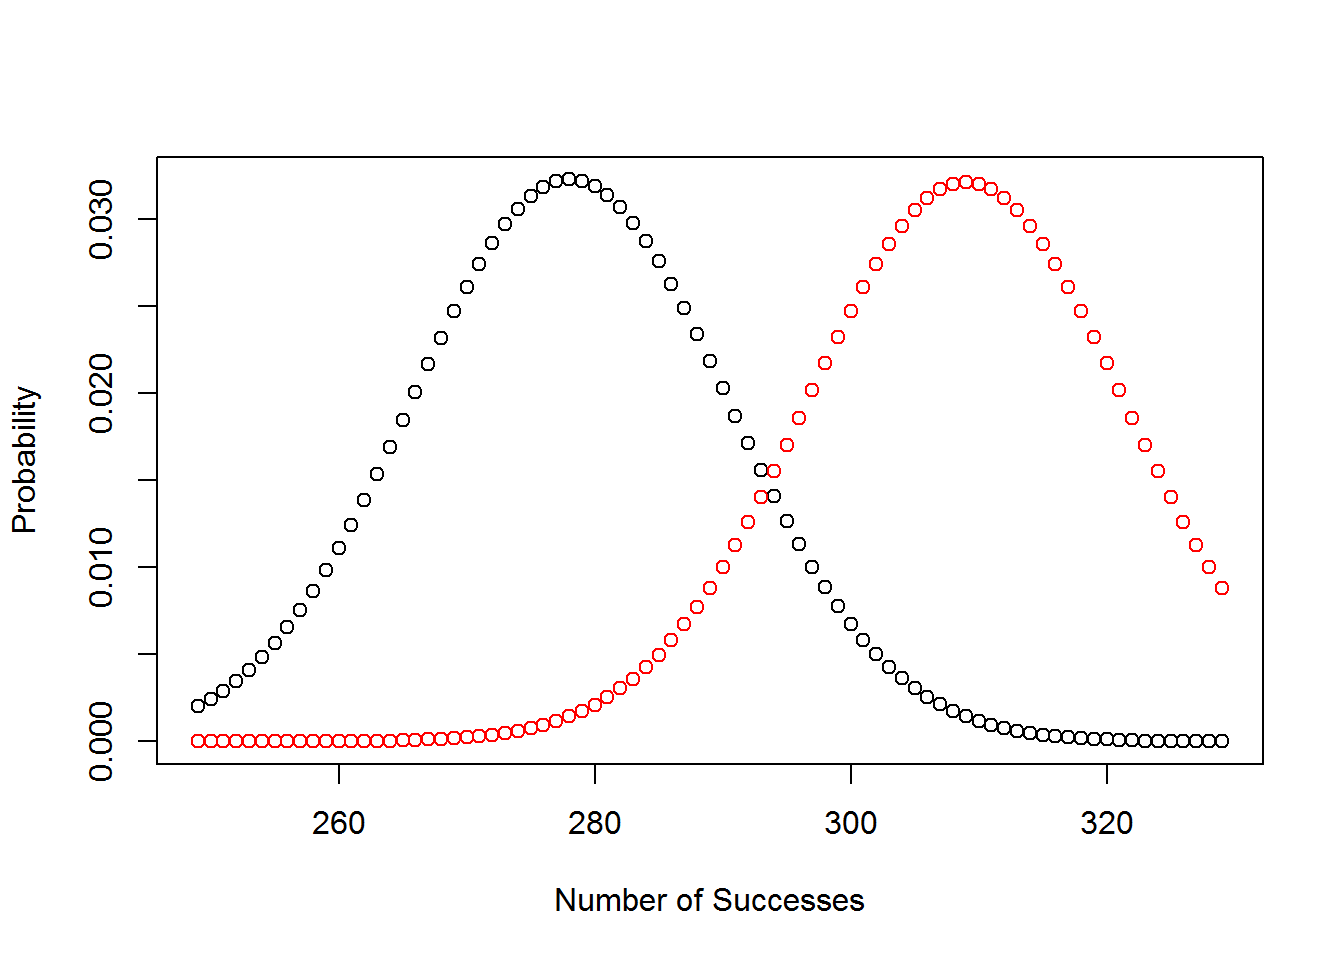
\includegraphics{fastR-Notes_files/figure-latex/unnamed-chunk-83-1.pdf}

\subsection{Complex Hypothesis}\label{complex-hypothesis}

The book goes through an example so we will keep it short here. Suppose
our hypotheses were

\[H_{o}:\pi=.45\] \[H_{o}:\pi\neq.45\]

The alternative is complex because it takes on many values. This
particular test is two-sided and is the most common. A one-sided test
can only be done if apriori you have knowledge that the parameter will
be on one side of the null hypothesized value.

To conduct this test, we can use the function \texttt{binom.test}.

\begin{Shaded}
\begin{Highlighting}[]
\KeywordTok{binom.test}\NormalTok{(}\DecValTok{49}\NormalTok{,}\DecValTok{100}\NormalTok{,}\DataTypeTok{p=}\NormalTok{.}\DecValTok{45}\NormalTok{,}\DataTypeTok{conf.level =}\NormalTok{ .}\DecValTok{05}\NormalTok{)}
\end{Highlighting}
\end{Shaded}

\begin{verbatim}
## 
## 
## 
## data:  49 out of 100
## number of successes = 49, number of trials = 100, p-value = 0.4235
## alternative hypothesis: true probability of success is not equal to 0.45
## 5 percent confidence interval:
##  0.4819244 0.4981442
## sample estimates:
## probability of success 
##                   0.49
\end{verbatim}

Again, we fail to reject.

To find power, you need a specified difference or size of effect that
you think is practically important, usually from a subject matter
expert. Let's say that expert wants to detect a difference of 0.05, this
is called the effect size. We now need a value for the alternative. We
could pick either 0.40 or 0.50. Let's go with 0.50. You could do both
and report the two power calculations back to the decision maker.

Since it is a two-sided test, we need to split the significance level
between both tails. Thus the critical values, the values that define the
rejection region are.

\begin{Shaded}
\begin{Highlighting}[]
\KeywordTok{qbinom}\NormalTok{(.}\DecValTok{975}\NormalTok{,}\DecValTok{100}\NormalTok{,.}\DecValTok{45}\NormalTok{)}
\end{Highlighting}
\end{Shaded}

\begin{verbatim}
## [1] 55
\end{verbatim}

\begin{Shaded}
\begin{Highlighting}[]
\KeywordTok{qbinom}\NormalTok{(.}\DecValTok{025}\NormalTok{,}\DecValTok{100}\NormalTok{,.}\DecValTok{45}\NormalTok{)}
\end{Highlighting}
\end{Shaded}

\begin{verbatim}
## [1] 35
\end{verbatim}

Again, since the distribution is discrete, it is unlikely that these
values will give us the exact probabilities we want. Let's check and
decide what we want to use.

\begin{Shaded}
\begin{Highlighting}[]
\DecValTok{1}\OperatorTok{-}\KeywordTok{pbinom}\NormalTok{(}\DecValTok{54}\OperatorTok{:}\DecValTok{56}\NormalTok{,}\DecValTok{100}\NormalTok{,.}\DecValTok{45}\NormalTok{)}
\end{Highlighting}
\end{Shaded}

\begin{verbatim}
## [1] 0.02839342 0.01764065 0.01057105
\end{verbatim}

\begin{Shaded}
\begin{Highlighting}[]
\KeywordTok{pbinom}\NormalTok{(}\DecValTok{34}\OperatorTok{:}\DecValTok{36}\NormalTok{,}\DecValTok{100}\NormalTok{,.}\DecValTok{45}\NormalTok{)}
\end{Highlighting}
\end{Shaded}

\begin{verbatim}
## [1] 0.01663269 0.02723630 0.04290071
\end{verbatim}

If we reject when we have 34 or fewer heads and 56 or greater heads then
the probability of a type I error is

\begin{Shaded}
\begin{Highlighting}[]
\DecValTok{1}\OperatorTok{-}\NormalTok{(}\KeywordTok{pbinom}\NormalTok{(}\DecValTok{55}\NormalTok{,}\DecValTok{100}\NormalTok{,.}\DecValTok{45}\NormalTok{)}\OperatorTok{-}\KeywordTok{pbinom}\NormalTok{(}\DecValTok{34}\NormalTok{,}\DecValTok{100}\NormalTok{,.}\DecValTok{45}\NormalTok{))}
\end{Highlighting}
\end{Shaded}

\begin{verbatim}
## [1] 0.03427334
\end{verbatim}

This is conservative and less that \texttt{0.05}. We could adjust a
little

\begin{Shaded}
\begin{Highlighting}[]
\DecValTok{1}\OperatorTok{-}\NormalTok{(}\KeywordTok{pbinom}\NormalTok{(}\DecValTok{55}\NormalTok{,}\DecValTok{100}\NormalTok{,.}\DecValTok{45}\NormalTok{)}\OperatorTok{-}\KeywordTok{pbinom}\NormalTok{(}\DecValTok{35}\NormalTok{,}\DecValTok{100}\NormalTok{,.}\DecValTok{45}\NormalTok{))}
\end{Highlighting}
\end{Shaded}

\begin{verbatim}
## [1] 0.04487694
\end{verbatim}

It is up to you to decide. Let's go with the second set. We reject if we
have 35 or fewer or 56 and greater heads. Now to find power, we
calculate the probability of rejecting given that the alternative is
true, which we have selected as 0.05.

\begin{Shaded}
\begin{Highlighting}[]
\DecValTok{1}\OperatorTok{-}\NormalTok{(}\KeywordTok{pbinom}\NormalTok{(}\DecValTok{55}\NormalTok{,}\DecValTok{100}\NormalTok{,.}\DecValTok{5}\NormalTok{)}\OperatorTok{-}\KeywordTok{pbinom}\NormalTok{(}\DecValTok{35}\NormalTok{,}\DecValTok{100}\NormalTok{,.}\DecValTok{5}\NormalTok{))}
\end{Highlighting}
\end{Shaded}

\begin{verbatim}
## [1] 0.1373853
\end{verbatim}

The power is small and thus to detect a difference of 0.05, we need a
larger sample size than 100.

For interest, let's check the power if the alternative were 0.40.

\begin{Shaded}
\begin{Highlighting}[]
\DecValTok{1}\OperatorTok{-}\NormalTok{(}\KeywordTok{pbinom}\NormalTok{(}\DecValTok{55}\NormalTok{,}\DecValTok{100}\NormalTok{,.}\DecValTok{4}\NormalTok{)}\OperatorTok{-}\KeywordTok{pbinom}\NormalTok{(}\DecValTok{35}\NormalTok{,}\DecValTok{100}\NormalTok{,.}\DecValTok{4}\NormalTok{))}
\end{Highlighting}
\end{Shaded}

\begin{verbatim}
## [1] 0.1803512
\end{verbatim}

\hypertarget{L9}{\section{Mean and Variance of Discrete Random
Variable}\label{L9}}

\subsection{Objectives}\label{objectives-8}

\begin{enumerate}
\def\labelenumi{\arabic{enumi}.}
\tightlist
\item
  Know and use definitions and properties of E(X) and V(X)\\
\item
  Find the pmf of the transformation of a random variable\\
\item
  Know E(X) and V(X) for common distributions
\end{enumerate}

\subsection{Review}\label{review}

Definitions you should know cold:

p-value: Probability of the observed data or more extreme given the null
hypothesis is true Level of significance (\(\alpha\)): The probability
of rejecting given the null hypothesis is true\\
Power: The probability of rejecting given that the alternative
hypothesis is true\\
\(\beta\): 1 - Power, the probability of failing to reject given that
the alternative hypothesis is true

\subsubsection{Practice problems}\label{practice-problems}

\begin{enumerate}
\def\labelenumi{\arabic{enumi}.}
\tightlist
\item
  We are testing if a die is fair by rolling it 30 time and recording
  the number of times one appears. The hypothesis is
  \[H_{o}:\pi={1 \over 6}\] \[H_{a}:\pi \neq {1 \over 6}\]
\end{enumerate}

The test statistic is 2. Using a significance level of \(\alpha\) =
0.05. Find the power of the test using an alternative probability of
success of 0.20.

\begin{enumerate}
\def\labelenumi{\arabic{enumi}.}
\setcounter{enumi}{1}
\tightlist
\item
  Let \(X\sim Binom(15,.25)\) Find \(P(X=2)\),\(P(X<7)\),\(P(X\geq8)\),
  and \(P(5<X\leq9)\)
\end{enumerate}

\subsection{Problem}\label{problem}

A random process flips a fair coin four times. Find the pmf for the
random variable \(Z\) = the difference between the number of heads and
the number of tails.

The values that z can take are -4, -2, 0, 2, and 4. The pmf will be the
same as the pmf for a binomial of four flips. Thus

\begin{Shaded}
\begin{Highlighting}[]
\KeywordTok{dbinom}\NormalTok{(}\DecValTok{0}\OperatorTok{:}\DecValTok{4}\NormalTok{,}\DecValTok{4}\NormalTok{,.}\DecValTok{5}\NormalTok{)}
\end{Highlighting}
\end{Shaded}

\begin{verbatim}
## [1] 0.0625 0.2500 0.3750 0.2500 0.0625
\end{verbatim}

If I install the \texttt{MASS} library, I can make these fractions.

\begin{Shaded}
\begin{Highlighting}[]
\KeywordTok{library}\NormalTok{(MASS)}
\end{Highlighting}
\end{Shaded}

\begin{Shaded}
\begin{Highlighting}[]
\KeywordTok{fractions}\NormalTok{(}\KeywordTok{dbinom}\NormalTok{(}\DecValTok{0}\OperatorTok{:}\DecValTok{4}\NormalTok{,}\DecValTok{4}\NormalTok{,.}\DecValTok{5}\NormalTok{))}
\end{Highlighting}
\end{Shaded}

\begin{verbatim}
## [1] 1/16  1/4  3/8  1/4 1/16
\end{verbatim}

\begin{enumerate}
\def\labelenumi{\arabic{enumi}.}
\tightlist
\item
  Find \(E(Z)\)
\end{enumerate}

By definition \(E(Z)=\sum_{z}zf(z)\)

\begin{Shaded}
\begin{Highlighting}[]
\KeywordTok{seq}\NormalTok{(}\OperatorTok{-}\DecValTok{4}\NormalTok{,}\DecValTok{4}\NormalTok{,}\DecValTok{2}\NormalTok{)}\OperatorTok{*}\KeywordTok{fractions}\NormalTok{(}\KeywordTok{dbinom}\NormalTok{(}\DecValTok{0}\OperatorTok{:}\DecValTok{4}\NormalTok{,}\DecValTok{4}\NormalTok{,.}\DecValTok{5}\NormalTok{))}
\end{Highlighting}
\end{Shaded}

\begin{verbatim}
## [1] -1/4 -1/2    0  1/2  1/4
\end{verbatim}

\begin{Shaded}
\begin{Highlighting}[]
\KeywordTok{sum}\NormalTok{(}\KeywordTok{seq}\NormalTok{(}\OperatorTok{-}\DecValTok{4}\NormalTok{,}\DecValTok{4}\NormalTok{,}\DecValTok{2}\NormalTok{)}\OperatorTok{*}\KeywordTok{fractions}\NormalTok{(}\KeywordTok{dbinom}\NormalTok{(}\DecValTok{0}\OperatorTok{:}\DecValTok{4}\NormalTok{,}\DecValTok{4}\NormalTok{,.}\DecValTok{5}\NormalTok{)))}
\end{Highlighting}
\end{Shaded}

\begin{verbatim}
## [1] 0
\end{verbatim}

The expected value, the average value of the population, is zero.

\begin{enumerate}
\def\labelenumi{\arabic{enumi}.}
\setcounter{enumi}{1}
\tightlist
\item
  Now a transformation, let \(Y=|Z|\). Find the pmf of \(Y\) and
  \(E(Y)\).
\end{enumerate}

This is an important definition:

Let \(X\) be a random variable and
\(t:\mathbb{R}\rightarrow \mathbb{R}\), then \(E(t(X))\) is
\(E(t(X))=\sum_{x}t(x)f(x)\)

The pmf is

\begin{Shaded}
\begin{Highlighting}[]
\NormalTok{temp<-}\KeywordTok{fractions}\NormalTok{(}\KeywordTok{c}\NormalTok{(}\KeywordTok{dbinom}\NormalTok{(}\DecValTok{2}\NormalTok{,}\DecValTok{4}\NormalTok{,.}\DecValTok{5}\NormalTok{),(}\KeywordTok{dbinom}\NormalTok{(}\DecValTok{1}\NormalTok{,}\DecValTok{4}\NormalTok{,.}\DecValTok{5}\NormalTok{)}\OperatorTok{+}\KeywordTok{dbinom}\NormalTok{(}\DecValTok{3}\NormalTok{,}\DecValTok{4}\NormalTok{,.}\DecValTok{5}\NormalTok{)),}\KeywordTok{dbinom}\NormalTok{(}\DecValTok{0}\NormalTok{,}\DecValTok{4}\NormalTok{,.}\DecValTok{5}\NormalTok{)}\OperatorTok{+}\KeywordTok{dbinom}\NormalTok{(}\DecValTok{0}\NormalTok{,}\DecValTok{4}\NormalTok{,.}\DecValTok{5}\NormalTok{)))}
\KeywordTok{names}\NormalTok{(temp)<-}\KeywordTok{c}\NormalTok{(}\DecValTok{0}\NormalTok{,}\DecValTok{2}\NormalTok{,}\DecValTok{4}\NormalTok{)}
\NormalTok{temp}
\end{Highlighting}
\end{Shaded}

\begin{verbatim}
##   0   2   4 
## 3/8 1/2 1/8
\end{verbatim}

The expected value is

\begin{Shaded}
\begin{Highlighting}[]
\KeywordTok{sum}\NormalTok{(}\KeywordTok{c}\NormalTok{(}\DecValTok{0}\NormalTok{,}\DecValTok{2}\NormalTok{,}\DecValTok{4}\NormalTok{)}\OperatorTok{*}\NormalTok{temp)}
\end{Highlighting}
\end{Shaded}

\begin{verbatim}
## [1] 3/2
\end{verbatim}

or

\begin{Shaded}
\begin{Highlighting}[]
\KeywordTok{fractions}\NormalTok{(}\KeywordTok{sum}\NormalTok{(}\KeywordTok{abs}\NormalTok{(}\KeywordTok{seq}\NormalTok{(}\OperatorTok{-}\DecValTok{4}\NormalTok{,}\DecValTok{4}\NormalTok{,}\DecValTok{2}\NormalTok{))}\OperatorTok{*}\KeywordTok{dbinom}\NormalTok{(}\DecValTok{0}\OperatorTok{:}\DecValTok{4}\NormalTok{,}\DecValTok{4}\NormalTok{,.}\DecValTok{5}\NormalTok{)))}
\end{Highlighting}
\end{Shaded}

\begin{verbatim}
## [1] 3/2
\end{verbatim}

\begin{enumerate}
\def\labelenumi{\arabic{enumi}.}
\setcounter{enumi}{2}
\tightlist
\item
  Find \(E(Z^2)\)
\end{enumerate}

The pmf is

\begin{Shaded}
\begin{Highlighting}[]
\NormalTok{temp<-}\KeywordTok{fractions}\NormalTok{(}\KeywordTok{c}\NormalTok{(}\KeywordTok{dbinom}\NormalTok{(}\DecValTok{2}\NormalTok{,}\DecValTok{4}\NormalTok{,.}\DecValTok{5}\NormalTok{),(}\KeywordTok{dbinom}\NormalTok{(}\DecValTok{1}\NormalTok{,}\DecValTok{4}\NormalTok{,.}\DecValTok{5}\NormalTok{)}\OperatorTok{+}\KeywordTok{dbinom}\NormalTok{(}\DecValTok{3}\NormalTok{,}\DecValTok{4}\NormalTok{,.}\DecValTok{5}\NormalTok{)),}\KeywordTok{dbinom}\NormalTok{(}\DecValTok{0}\NormalTok{,}\DecValTok{4}\NormalTok{,.}\DecValTok{5}\NormalTok{)}\OperatorTok{+}\KeywordTok{dbinom}\NormalTok{(}\DecValTok{0}\NormalTok{,}\DecValTok{4}\NormalTok{,.}\DecValTok{5}\NormalTok{)))}
\KeywordTok{names}\NormalTok{(temp)<-}\KeywordTok{c}\NormalTok{(}\DecValTok{0}\NormalTok{,}\DecValTok{4}\NormalTok{,}\DecValTok{16}\NormalTok{)}
\NormalTok{temp}
\end{Highlighting}
\end{Shaded}

\begin{verbatim}
##   0   4  16 
## 3/8 1/2 1/8
\end{verbatim}

The expected value is

\begin{Shaded}
\begin{Highlighting}[]
\KeywordTok{sum}\NormalTok{(}\KeywordTok{c}\NormalTok{(}\DecValTok{0}\NormalTok{,}\DecValTok{4}\NormalTok{,}\DecValTok{16}\NormalTok{)}\OperatorTok{*}\NormalTok{temp)}
\end{Highlighting}
\end{Shaded}

\begin{verbatim}
## [1] 4
\end{verbatim}

or

\begin{Shaded}
\begin{Highlighting}[]
\KeywordTok{fractions}\NormalTok{(}\KeywordTok{sum}\NormalTok{((}\KeywordTok{seq}\NormalTok{(}\OperatorTok{-}\DecValTok{4}\NormalTok{,}\DecValTok{4}\NormalTok{,}\DecValTok{2}\NormalTok{)}\OperatorTok{^}\DecValTok{2}\NormalTok{)}\OperatorTok{*}\KeywordTok{dbinom}\NormalTok{(}\DecValTok{0}\OperatorTok{:}\DecValTok{4}\NormalTok{,}\DecValTok{4}\NormalTok{,.}\DecValTok{5}\NormalTok{)))}
\end{Highlighting}
\end{Shaded}

\begin{verbatim}
## [1] 4
\end{verbatim}

\begin{enumerate}
\def\labelenumi{\arabic{enumi}.}
\setcounter{enumi}{3}
\tightlist
\item
  Variance is just an expected value and is defined as
  \[Var(X)=E((X-E(X))^2)\] where \(E(X)\) is sometimes denoted as
  \(\mu\)
\end{enumerate}

by definition:
\[E((X-E(X))^2)=E((X-\mu)^2)=\sum_{x}t(x)f(x)=\sum_{x}(x-\mu)^2f(x)\]

find \(Var(Z)\)

\begin{Shaded}
\begin{Highlighting}[]
\NormalTok{(}\KeywordTok{seq}\NormalTok{(}\OperatorTok{-}\DecValTok{4}\NormalTok{,}\DecValTok{4}\NormalTok{,}\DecValTok{2}\NormalTok{)}\OperatorTok{-}\DecValTok{0}\NormalTok{)}\OperatorTok{^}\DecValTok{2}\OperatorTok{*}\KeywordTok{fractions}\NormalTok{(}\KeywordTok{dbinom}\NormalTok{(}\DecValTok{0}\OperatorTok{:}\DecValTok{4}\NormalTok{,}\DecValTok{4}\NormalTok{,.}\DecValTok{5}\NormalTok{))}
\end{Highlighting}
\end{Shaded}

\begin{verbatim}
## [1] 1 1 0 1 1
\end{verbatim}

\begin{Shaded}
\begin{Highlighting}[]
\KeywordTok{sum}\NormalTok{((}\KeywordTok{seq}\NormalTok{(}\OperatorTok{-}\DecValTok{4}\NormalTok{,}\DecValTok{4}\NormalTok{,}\DecValTok{2}\NormalTok{)}\OperatorTok{-}\DecValTok{0}\NormalTok{)}\OperatorTok{^}\DecValTok{2}\OperatorTok{*}\KeywordTok{fractions}\NormalTok{(}\KeywordTok{dbinom}\NormalTok{(}\DecValTok{0}\OperatorTok{:}\DecValTok{4}\NormalTok{,}\DecValTok{4}\NormalTok{,.}\DecValTok{5}\NormalTok{)))}
\end{Highlighting}
\end{Shaded}

\begin{verbatim}
## [1] 4
\end{verbatim}

You can also find variance using \[Var(X)=E(X^2)-E(X)^2\]

\begin{enumerate}
\def\labelenumi{\arabic{enumi}.}
\setcounter{enumi}{4}
\tightlist
\item
  Other properties \[E(aX+b)=aE(X)+b\] \[Var(aX+b)=a^2Var(X)\]
\end{enumerate}

Do Homework problem 2.64

\hypertarget{L10}{\section{Discrete Joint Distributions}\label{L10}}

\subsection{Objectives}\label{objectives-9}

\begin{enumerate}
\def\labelenumi{\arabic{enumi}.}
\tightlist
\item
  Know and use definitions such as joint pmf, conditional distribution,
  marginal distribution, independence, covariance, and correlation
  coefficient\\
\item
  Find the various probability mass functions (joint, marginal, and
  conditional)\\
\item
  Know and use properties of E(X),V(X), and Cov(X,Y) for sums and
  products of random variables
\end{enumerate}

\subsection{Example}\label{example}

Consider a contrived example of three random variables X, Y, and Z. The
following is the joint probability mass function

\begin{Shaded}
\begin{Highlighting}[]
\KeywordTok{library}\NormalTok{(MASS)}
\end{Highlighting}
\end{Shaded}

\begin{Shaded}
\begin{Highlighting}[]
\KeywordTok{fractions}\NormalTok{(Les10ex<-}\KeywordTok{array}\NormalTok{(}\KeywordTok{c}\NormalTok{(}\DecValTok{3}\OperatorTok{/}\DecValTok{64}\NormalTok{,}\DecValTok{9}\OperatorTok{/}\DecValTok{64}\NormalTok{,}\DecValTok{9}\OperatorTok{/}\DecValTok{64}\NormalTok{,}\DecValTok{27}\OperatorTok{/}\DecValTok{64}\NormalTok{,}\DecValTok{2}\OperatorTok{/}\DecValTok{64}\NormalTok{,}\DecValTok{6}\OperatorTok{/}\DecValTok{64}\NormalTok{,}\DecValTok{2}\OperatorTok{/}\DecValTok{64}\NormalTok{,}\DecValTok{6}\OperatorTok{/}\DecValTok{64}\NormalTok{),}\DataTypeTok{dim=}\KeywordTok{c}\NormalTok{(}\DecValTok{2}\NormalTok{,}\DecValTok{2}\NormalTok{,}\DecValTok{2}\NormalTok{),}\DataTypeTok{dimnames =} \KeywordTok{list}\NormalTok{(}\KeywordTok{c}\NormalTok{(}\DecValTok{0}\NormalTok{,}\DecValTok{1}\NormalTok{),}\KeywordTok{c}\NormalTok{(}\DecValTok{0}\NormalTok{,}\DecValTok{1}\NormalTok{),}\KeywordTok{c}\NormalTok{(}\DecValTok{0}\NormalTok{,}\DecValTok{1}\NormalTok{))))}
\end{Highlighting}
\end{Shaded}

\begin{verbatim}
## , , 0
## 
##   0     1    
## 0  3/64  9/64
## 1  9/64 27/64
## 
## , , 1
## 
##   0     1    
## 0  1/32  1/32
## 1  3/32  3/32
\end{verbatim}

This might be easier to look at:

\begin{Shaded}
\begin{Highlighting}[]
\NormalTok{Les10exa<-}\KeywordTok{data.frame}\NormalTok{(}\DataTypeTok{X=}\KeywordTok{c}\NormalTok{(}\KeywordTok{rep}\NormalTok{(}\DecValTok{0}\NormalTok{,}\DecValTok{16}\NormalTok{),}\KeywordTok{rep}\NormalTok{(}\DecValTok{1}\NormalTok{,}\DecValTok{48}\NormalTok{)),}\DataTypeTok{Y=}\KeywordTok{c}\NormalTok{(}\DecValTok{0}\NormalTok{,}\DecValTok{0}\NormalTok{,}\DecValTok{0}\NormalTok{,}\KeywordTok{rep}\NormalTok{(}\DecValTok{1}\NormalTok{,}\DecValTok{9}\NormalTok{),}\KeywordTok{rep}\NormalTok{(}\KeywordTok{c}\NormalTok{(}\DecValTok{0}\NormalTok{,}\DecValTok{1}\NormalTok{),}\DataTypeTok{each=}\DecValTok{2}\NormalTok{),}\KeywordTok{rep}\NormalTok{(}\DecValTok{0}\NormalTok{,}\DecValTok{9}\NormalTok{),}\KeywordTok{rep}\NormalTok{(}\DecValTok{1}\NormalTok{,}\DecValTok{27}\NormalTok{),}\KeywordTok{rep}\NormalTok{(}\KeywordTok{c}\NormalTok{(}\DecValTok{0}\NormalTok{,}\DecValTok{1}\NormalTok{),}\DataTypeTok{each=}\DecValTok{6}\NormalTok{)),}\DataTypeTok{Z=}\KeywordTok{c}\NormalTok{(}\KeywordTok{rep}\NormalTok{(}\DecValTok{0}\NormalTok{,}\DecValTok{12}\NormalTok{),}\KeywordTok{rep}\NormalTok{(}\DecValTok{1}\NormalTok{,}\DecValTok{4}\NormalTok{),}\KeywordTok{rep}\NormalTok{(}\DecValTok{0}\NormalTok{,}\DecValTok{36}\NormalTok{),}\KeywordTok{rep}\NormalTok{(}\DecValTok{1}\NormalTok{,}\DecValTok{12}\NormalTok{)))}
\end{Highlighting}
\end{Shaded}

Now we have our pmf

\begin{Shaded}
\begin{Highlighting}[]
\KeywordTok{fractions}\NormalTok{(}\KeywordTok{prop.table}\NormalTok{(}\KeywordTok{table}\NormalTok{(Les10exa)))}
\end{Highlighting}
\end{Shaded}

\begin{verbatim}
## , , Z = 0
## 
##    Y
## X   0     1    
##   0  3/64  9/64
##   1  9/64 27/64
## 
## , , Z = 1
## 
##    Y
## X   0     1    
##   0  1/32  1/32
##   1  3/32  3/32
\end{verbatim}

Notice this is a pmf since each value is between 0 and 1 and the sum is
1.

That is \(\sum_{x,y,z}f_{XYZ}(x,y,z)=1\).

\begin{Shaded}
\begin{Highlighting}[]
\KeywordTok{sum}\NormalTok{(}\KeywordTok{fractions}\NormalTok{(}\KeywordTok{prop.table}\NormalTok{(}\KeywordTok{table}\NormalTok{(Les10exa))))}
\end{Highlighting}
\end{Shaded}

\begin{verbatim}
## [1] 1
\end{verbatim}

\subsection{Problem 1}\label{problem-1}

\begin{enumerate}
\def\labelenumi{\arabic{enumi}.}
\tightlist
\item
  Find \(P(X=1,Y=1,Z=1)\) which is \(f_{XYZ}(1,1,1)\). Notice that we
  are using a comma instead of the intersection symbol. This is to make
  the notation easier.
\end{enumerate}

The answer is \texttt{6/64}. This is a joint probability.

\begin{enumerate}
\def\labelenumi{\arabic{enumi}.}
\setcounter{enumi}{1}
\tightlist
\item
  Find the marginal pmf of X.
\end{enumerate}

\begin{Shaded}
\begin{Highlighting}[]
\KeywordTok{fractions}\NormalTok{(}\KeywordTok{apply}\NormalTok{(}\KeywordTok{prop.table}\NormalTok{(}\KeywordTok{table}\NormalTok{(Les10exa)),}\DecValTok{1}\NormalTok{,sum))}
\end{Highlighting}
\end{Shaded}

\begin{verbatim}
##   0   1 
## 1/4 3/4
\end{verbatim}

\begin{enumerate}
\def\labelenumi{\arabic{enumi}.}
\setcounter{enumi}{2}
\tightlist
\item
  Find \(E(X)\)
\end{enumerate}

\begin{Shaded}
\begin{Highlighting}[]
\KeywordTok{sum}\NormalTok{(}\KeywordTok{apply}\NormalTok{(}\KeywordTok{fractions}\NormalTok{(}\KeywordTok{prop.table}\NormalTok{(}\KeywordTok{table}\NormalTok{(Les10exa))),}\DecValTok{1}\NormalTok{,sum)}\OperatorTok{*}\KeywordTok{c}\NormalTok{(}\DecValTok{0}\NormalTok{,}\DecValTok{1}\NormalTok{))}
\end{Highlighting}
\end{Shaded}

\begin{verbatim}
## [1] 0.75
\end{verbatim}

\begin{enumerate}
\def\labelenumi{\arabic{enumi}.}
\setcounter{enumi}{3}
\tightlist
\item
  Find \(f_{XY}(x,y)\).
\end{enumerate}

\begin{Shaded}
\begin{Highlighting}[]
\KeywordTok{fractions}\NormalTok{(}\KeywordTok{apply}\NormalTok{(}\KeywordTok{prop.table}\NormalTok{(}\KeywordTok{table}\NormalTok{(Les10exa)),}\DecValTok{1}\OperatorTok{:}\DecValTok{2}\NormalTok{,sum))}
\end{Highlighting}
\end{Shaded}

\begin{verbatim}
##    Y
## X   0     1    
##   0  5/64 11/64
##   1 15/64 33/64
\end{verbatim}

\begin{enumerate}
\def\labelenumi{\arabic{enumi}.}
\setcounter{enumi}{4}
\tightlist
\item
  Are \(X\) and \(Y\) independent?
\end{enumerate}

We need to verify that \(f_{XY}(x,y)=f_{X}(x)f_{Y}(y)\) for all \(x\)
and \(y\).

We need \(f_{X}(x)\) and \(f_{Y}(y)\)

\begin{Shaded}
\begin{Highlighting}[]
\KeywordTok{fractions}\NormalTok{(}\KeywordTok{apply}\NormalTok{(}\KeywordTok{prop.table}\NormalTok{(}\KeywordTok{table}\NormalTok{(Les10exa)),}\DecValTok{1}\NormalTok{,sum))}
\end{Highlighting}
\end{Shaded}

\begin{verbatim}
##   0   1 
## 1/4 3/4
\end{verbatim}

\begin{Shaded}
\begin{Highlighting}[]
\KeywordTok{fractions}\NormalTok{(}\KeywordTok{apply}\NormalTok{(}\KeywordTok{prop.table}\NormalTok{(}\KeywordTok{table}\NormalTok{(Les10exa)),}\DecValTok{2}\NormalTok{,sum))}
\end{Highlighting}
\end{Shaded}

\begin{verbatim}
##     0     1 
##  5/16 11/16
\end{verbatim}

We could multiply these one at a time or use an outer product to make it
easier

\begin{Shaded}
\begin{Highlighting}[]
\KeywordTok{fractions}\NormalTok{(}\KeywordTok{outer}\NormalTok{(}\KeywordTok{apply}\NormalTok{(}\KeywordTok{prop.table}\NormalTok{(}\KeywordTok{table}\NormalTok{(Les10exa)),}\DecValTok{1}\NormalTok{,sum),}\KeywordTok{apply}\NormalTok{(}\KeywordTok{prop.table}\NormalTok{(}\KeywordTok{table}\NormalTok{(Les10exa)),}\DecValTok{2}\NormalTok{,sum)))}
\end{Highlighting}
\end{Shaded}

\begin{verbatim}
##   0     1    
## 0  5/64 11/64
## 1 15/64 33/64
\end{verbatim}

The joint pmf is

\begin{Shaded}
\begin{Highlighting}[]
\KeywordTok{fractions}\NormalTok{(}\KeywordTok{apply}\NormalTok{(}\KeywordTok{prop.table}\NormalTok{(}\KeywordTok{table}\NormalTok{(Les10exa)),}\DecValTok{1}\OperatorTok{:}\DecValTok{2}\NormalTok{,sum))}
\end{Highlighting}
\end{Shaded}

\begin{verbatim}
##    Y
## X   0     1    
##   0  5/64 11/64
##   1 15/64 33/64
\end{verbatim}

They are equal so \(X\) and \(Y\) are independent.

\begin{enumerate}
\def\labelenumi{\arabic{enumi}.}
\setcounter{enumi}{4}
\tightlist
\item
  How about \(X\) and \(Z\)?
\end{enumerate}

\begin{Shaded}
\begin{Highlighting}[]
\KeywordTok{fractions}\NormalTok{(}\KeywordTok{apply}\NormalTok{(}\KeywordTok{prop.table}\NormalTok{(}\KeywordTok{table}\NormalTok{(Les10exa)),}\DecValTok{1}\NormalTok{,sum))}
\end{Highlighting}
\end{Shaded}

\begin{verbatim}
##   0   1 
## 1/4 3/4
\end{verbatim}

\begin{Shaded}
\begin{Highlighting}[]
\KeywordTok{fractions}\NormalTok{(}\KeywordTok{apply}\NormalTok{(}\KeywordTok{prop.table}\NormalTok{(}\KeywordTok{table}\NormalTok{(Les10exa)),}\DecValTok{3}\NormalTok{,sum))}
\end{Highlighting}
\end{Shaded}

\begin{verbatim}
##   0   1 
## 3/4 1/4
\end{verbatim}

\begin{Shaded}
\begin{Highlighting}[]
\KeywordTok{fractions}\NormalTok{(}\KeywordTok{outer}\NormalTok{(}\KeywordTok{apply}\NormalTok{(}\KeywordTok{prop.table}\NormalTok{(}\KeywordTok{table}\NormalTok{(Les10exa)),}\DecValTok{1}\NormalTok{,sum),}\KeywordTok{apply}\NormalTok{(}\KeywordTok{prop.table}\NormalTok{(}\KeywordTok{table}\NormalTok{(Les10exa)),}\DecValTok{3}\NormalTok{,sum)))}
\end{Highlighting}
\end{Shaded}

\begin{verbatim}
##   0    1   
## 0 3/16 1/16
## 1 9/16 3/16
\end{verbatim}

The joint pmf is

\begin{Shaded}
\begin{Highlighting}[]
\KeywordTok{fractions}\NormalTok{(}\KeywordTok{apply}\NormalTok{(}\KeywordTok{prop.table}\NormalTok{(}\KeywordTok{table}\NormalTok{(Les10exa)),}\KeywordTok{c}\NormalTok{(}\DecValTok{1}\NormalTok{,}\DecValTok{3}\NormalTok{),sum))}
\end{Highlighting}
\end{Shaded}

\begin{verbatim}
##    Z
## X   0    1   
##   0 3/16 1/16
##   1 9/16 3/16
\end{verbatim}

Thus \(X\) and \(Z\) are independent.

\begin{enumerate}
\def\labelenumi{\arabic{enumi}.}
\setcounter{enumi}{5}
\tightlist
\item
  How about \(X\), \(Y\), and \(Z\)?
\end{enumerate}

If they are independent, then
\(f_{XYZ}(x,y,z)=f_{X}(x)f_{Y}(y)f_{Z}(z)\) for all \(x\), \(y\), and
\(z\).

\begin{Shaded}
\begin{Highlighting}[]
\KeywordTok{fractions}\NormalTok{(}\KeywordTok{apply}\NormalTok{(}\KeywordTok{prop.table}\NormalTok{(}\KeywordTok{table}\NormalTok{(Les10exa)),}\DecValTok{1}\NormalTok{,sum))}
\end{Highlighting}
\end{Shaded}

\begin{verbatim}
##   0   1 
## 1/4 3/4
\end{verbatim}

\begin{Shaded}
\begin{Highlighting}[]
\KeywordTok{fractions}\NormalTok{(}\KeywordTok{apply}\NormalTok{(}\KeywordTok{prop.table}\NormalTok{(}\KeywordTok{table}\NormalTok{(Les10exa)),}\DecValTok{2}\NormalTok{,sum))}
\end{Highlighting}
\end{Shaded}

\begin{verbatim}
##     0     1 
##  5/16 11/16
\end{verbatim}

\begin{Shaded}
\begin{Highlighting}[]
\KeywordTok{fractions}\NormalTok{(}\KeywordTok{apply}\NormalTok{(}\KeywordTok{prop.table}\NormalTok{(}\KeywordTok{table}\NormalTok{(Les10exa)),}\DecValTok{3}\NormalTok{,sum))}
\end{Highlighting}
\end{Shaded}

\begin{verbatim}
##   0   1 
## 3/4 1/4
\end{verbatim}

The product of the marginals is

\begin{Shaded}
\begin{Highlighting}[]
\KeywordTok{fractions}\NormalTok{(}\KeywordTok{outer}\NormalTok{(}\KeywordTok{outer}\NormalTok{(}\KeywordTok{apply}\NormalTok{(}\KeywordTok{prop.table}\NormalTok{(}\KeywordTok{table}\NormalTok{(Les10exa)),}\DecValTok{1}\NormalTok{,sum),}\KeywordTok{apply}\NormalTok{(}\KeywordTok{prop.table}\NormalTok{(}\KeywordTok{table}\NormalTok{(Les10exa)),}\DecValTok{2}\NormalTok{,sum)),}\KeywordTok{apply}\NormalTok{(}\KeywordTok{prop.table}\NormalTok{(}\KeywordTok{table}\NormalTok{(Les10exa)),}\DecValTok{3}\NormalTok{,sum)))}
\end{Highlighting}
\end{Shaded}

\begin{verbatim}
## , , 0
## 
##   0      1     
## 0 15/256 33/256
## 1 45/256 99/256
## 
## , , 1
## 
##   0      1     
## 0  5/256 11/256
## 1 15/256 33/256
\end{verbatim}

The joint pmf is

\begin{Shaded}
\begin{Highlighting}[]
\KeywordTok{fractions}\NormalTok{(}\KeywordTok{prop.table}\NormalTok{(}\KeywordTok{table}\NormalTok{(Les10exa)))}
\end{Highlighting}
\end{Shaded}

\begin{verbatim}
## , , Z = 0
## 
##    Y
## X   0     1    
##   0  3/64  9/64
##   1  9/64 27/64
## 
## , , Z = 1
## 
##    Y
## X   0     1    
##   0  1/32  1/32
##   1  3/32  3/32
\end{verbatim}

They are not independent.

In this problem we have pairwise independence but not independence.

\begin{enumerate}
\def\labelenumi{\arabic{enumi}.}
\setcounter{enumi}{6}
\tightlist
\item
  Find \(f_{X|Y=1}(x)\). This is a conditional pmf.
\end{enumerate}

From the definition of conditional probability
\[f_{X|Y=1}(x)={f_{XY}(x,y) \over f_{Y}(y)}|_{y=1}={f_{XY}(x,1) \over f_{Y}(1)}\]

The joint pmf of \(X\) and \(Y\) is

\begin{Shaded}
\begin{Highlighting}[]
\KeywordTok{fractions}\NormalTok{(}\KeywordTok{apply}\NormalTok{(}\KeywordTok{prop.table}\NormalTok{(}\KeywordTok{table}\NormalTok{(Les10exa)),}\DecValTok{1}\OperatorTok{:}\DecValTok{2}\NormalTok{,sum))}
\end{Highlighting}
\end{Shaded}

\begin{verbatim}
##    Y
## X   0     1    
##   0  5/64 11/64
##   1 15/64 33/64
\end{verbatim}

and the marginal of \(Y\) is

\begin{Shaded}
\begin{Highlighting}[]
\KeywordTok{fractions}\NormalTok{(}\KeywordTok{apply}\NormalTok{(}\KeywordTok{prop.table}\NormalTok{(}\KeywordTok{table}\NormalTok{(Les10exa)),}\DecValTok{2}\NormalTok{,sum))}
\end{Highlighting}
\end{Shaded}

\begin{verbatim}
##     0     1 
##  5/16 11/16
\end{verbatim}

Since \(y=1\) we want the second column of the joint

\begin{Shaded}
\begin{Highlighting}[]
\KeywordTok{fractions}\NormalTok{(}\KeywordTok{apply}\NormalTok{(}\KeywordTok{prop.table}\NormalTok{(}\KeywordTok{table}\NormalTok{(Les10exa)),}\DecValTok{1}\OperatorTok{:}\DecValTok{2}\NormalTok{,sum))[,}\DecValTok{2}\NormalTok{]}
\end{Highlighting}
\end{Shaded}

\begin{verbatim}
##     0     1 
## 11/64 33/64
\end{verbatim}

divided by the second element of the marginal

\begin{Shaded}
\begin{Highlighting}[]
\KeywordTok{fractions}\NormalTok{(}\KeywordTok{apply}\NormalTok{(}\KeywordTok{prop.table}\NormalTok{(}\KeywordTok{table}\NormalTok{(Les10exa)),}\DecValTok{2}\NormalTok{,sum))[}\DecValTok{2}\NormalTok{]}
\end{Highlighting}
\end{Shaded}

\begin{verbatim}
##     1 
## 11/16
\end{verbatim}

\begin{Shaded}
\begin{Highlighting}[]
\KeywordTok{fractions}\NormalTok{(}\KeywordTok{apply}\NormalTok{(}\KeywordTok{prop.table}\NormalTok{(}\KeywordTok{table}\NormalTok{(Les10exa)),}\DecValTok{1}\OperatorTok{:}\DecValTok{2}\NormalTok{,sum))[,}\DecValTok{2}\NormalTok{]}\OperatorTok{/}\KeywordTok{fractions}\NormalTok{(}\KeywordTok{apply}\NormalTok{(}\KeywordTok{prop.table}\NormalTok{(}\KeywordTok{table}\NormalTok{(Les10exa)),}\DecValTok{2}\NormalTok{,sum))[}\DecValTok{2}\NormalTok{]}
\end{Highlighting}
\end{Shaded}

\begin{verbatim}
##   0   1 
## 1/4 3/4
\end{verbatim}

Notice that since \(X\) and \(Y\) are independent, this is just the
marginal of \(X\)

\begin{Shaded}
\begin{Highlighting}[]
\KeywordTok{fractions}\NormalTok{(}\KeywordTok{apply}\NormalTok{(}\KeywordTok{prop.table}\NormalTok{(}\KeywordTok{table}\NormalTok{(Les10exa)),}\DecValTok{1}\NormalTok{,sum))}
\end{Highlighting}
\end{Shaded}

\begin{verbatim}
##   0   1 
## 1/4 3/4
\end{verbatim}

\subsection{Problem 2}\label{problem-2}

Let do a problem where the random variables are not independent.

\begin{Shaded}
\begin{Highlighting}[]
\NormalTok{Les10ex2<-}\KeywordTok{data.frame}\NormalTok{(}\DataTypeTok{X=}\KeywordTok{c}\NormalTok{(}\OperatorTok{-}\DecValTok{1}\NormalTok{,}\DecValTok{0}\NormalTok{,}\DecValTok{0}\NormalTok{,}\DecValTok{1}\NormalTok{),}\DataTypeTok{Y=}\KeywordTok{c}\NormalTok{(}\DecValTok{1}\NormalTok{,}\DecValTok{0}\NormalTok{,}\DecValTok{0}\NormalTok{,}\DecValTok{1}\NormalTok{))}
\end{Highlighting}
\end{Shaded}

Now we have our pmf

\begin{Shaded}
\begin{Highlighting}[]
\KeywordTok{fractions}\NormalTok{(}\KeywordTok{prop.table}\NormalTok{(}\KeywordTok{table}\NormalTok{(Les10ex2)))}
\end{Highlighting}
\end{Shaded}

\begin{verbatim}
##     Y
## X    0   1  
##   -1   0 1/4
##   0  1/2   0
##   1    0 1/4
\end{verbatim}

\begin{enumerate}
\def\labelenumi{\arabic{enumi}.}
\tightlist
\item
  Are \(X\) and \(Y\) independent?
\end{enumerate}

\begin{Shaded}
\begin{Highlighting}[]
\KeywordTok{fractions}\NormalTok{(}\KeywordTok{apply}\NormalTok{(}\KeywordTok{prop.table}\NormalTok{(}\KeywordTok{table}\NormalTok{(Les10ex2)),}\DecValTok{1}\NormalTok{,sum))}
\end{Highlighting}
\end{Shaded}

\begin{verbatim}
##  -1   0   1 
## 1/4 1/2 1/4
\end{verbatim}

\begin{Shaded}
\begin{Highlighting}[]
\KeywordTok{fractions}\NormalTok{(}\KeywordTok{apply}\NormalTok{(}\KeywordTok{prop.table}\NormalTok{(}\KeywordTok{table}\NormalTok{(Les10ex2)),}\DecValTok{2}\NormalTok{,sum))}
\end{Highlighting}
\end{Shaded}

\begin{verbatim}
##   0   1 
## 1/2 1/2
\end{verbatim}

\begin{Shaded}
\begin{Highlighting}[]
\KeywordTok{fractions}\NormalTok{(}\KeywordTok{outer}\NormalTok{(}\KeywordTok{fractions}\NormalTok{(}\KeywordTok{apply}\NormalTok{(}\KeywordTok{prop.table}\NormalTok{(}\KeywordTok{table}\NormalTok{(Les10ex2)),}\DecValTok{1}\NormalTok{,sum)),}\KeywordTok{fractions}\NormalTok{(}\KeywordTok{apply}\NormalTok{(}\KeywordTok{prop.table}\NormalTok{(}\KeywordTok{table}\NormalTok{(Les10ex2)),}\DecValTok{2}\NormalTok{,sum))))}
\end{Highlighting}
\end{Shaded}

\begin{verbatim}
##    0   1  
## -1 1/8 1/8
## 0  1/4 1/4
## 1  1/8 1/8
\end{verbatim}

This is not equal to the joint pmf, so they are not independent.

\begin{enumerate}
\def\labelenumi{\arabic{enumi}.}
\setcounter{enumi}{1}
\tightlist
\item
  Find Cov(\(X\),\(Y\)).
\end{enumerate}

By definition, this is \(E[(X-E(X))(Y-E(Y))]\).

Now \(E(X)\)=0 and \(E(Y)\)=1/2.

Now we can find the covariance, we do not need to write the product when
the joint probability is zero since the product will be zero. Thus we
have

\[(-1-0)(1-1/2)(1/4)+(0-0)(0-1/2)(1/2)+(1-0)(1-1/2)(1/4)=0\]

The covariance is zero even though \(X\) and \(Y\) are dependent. That
is because covariance measures a linear relationship. The relationship
here is purely quadratic with no linear component.

\begin{enumerate}
\def\labelenumi{\arabic{enumi}.}
\setcounter{enumi}{2}
\tightlist
\item
  Find \(E(XY)\)
\end{enumerate}

We need the pmf of \(W=XY\).

The random variable \(W\) can take on the values \(-1,0,1\) with
probabilities of \(1/4,1/2,1/4\). Thus the expected value is
\((1/4)(-1)+(1/2)(0)+(1/4)(1)=0\)

Notice that if random variables are independent, their covariance is
zero. The converse is not true.

We have another formula for covariance

\[Cov(X,Y)=E(XY)-E(X)E(Y)\]

We also now have \[Var(X,Y)=Var(X)+Var(Y)+2Cov(X,Y)\]

\subsection{Other}\label{other}

Make sure you know Thm 2.6.7, Lemma 2.6.13, and Lemma 2.6.14.

\begin{Shaded}
\begin{Highlighting}[]
\KeywordTok{library}\NormalTok{(fastR)}
\end{Highlighting}
\end{Shaded}

For an example, let's use the airline data from a previous lessons.
Let's assume this is the pmf and not empirical data.

\begin{Shaded}
\begin{Highlighting}[]
\KeywordTok{prop.table}\NormalTok{(}\KeywordTok{xtabs}\NormalTok{(}\OperatorTok{~}\NormalTok{Airport}\OperatorTok{+}\NormalTok{Airline}\OperatorTok{+}\NormalTok{Result,airlineArrival))}
\end{Highlighting}
\end{Shaded}

\begin{verbatim}
## , , Result = Delayed
## 
##               Airline
## Airport             Alaska AmericaWest
##   LosAngeles   0.005636364 0.010636364
##   Phoenix      0.001090909 0.037727273
##   SanDiego     0.001818182 0.005909091
##   SanFrancisco 0.009272727 0.011727273
##   Seattle      0.027727273 0.005545455
## 
## , , Result = OnTime
## 
##               Airline
## Airport             Alaska AmericaWest
##   LosAngeles   0.045181818 0.063090909
##   Phoenix      0.020090909 0.440000000
##   SanDiego     0.019272727 0.034818182
##   SanFrancisco 0.045727273 0.029090909
##   Seattle      0.167363636 0.018272727
\end{verbatim}

Now you can do the same work of finding marginal pmf, checking for
independence, finding conditional pmf, etc.

For example, the joint pmf for Airline and Result is:

\begin{Shaded}
\begin{Highlighting}[]
\KeywordTok{apply}\NormalTok{(}\KeywordTok{prop.table}\NormalTok{(}\KeywordTok{xtabs}\NormalTok{(}\OperatorTok{~}\NormalTok{Airport}\OperatorTok{+}\NormalTok{Airline}\OperatorTok{+}\NormalTok{Result,airlineArrival)),}\DecValTok{2}\OperatorTok{:}\DecValTok{3}\NormalTok{,sum)}
\end{Highlighting}
\end{Shaded}

\begin{verbatim}
##              Result
## Airline          Delayed    OnTime
##   Alaska      0.04554545 0.2976364
##   AmericaWest 0.07154545 0.5852727
\end{verbatim}

\hypertarget{L11}{\section{Other Discrete Distributions}\label{L11}}

\subsection{Objectives}\label{objectives-10}

\begin{enumerate}
\def\labelenumi{\arabic{enumi}.}
\tightlist
\item
  Know assumptions, parameters, E(X), V(X), and how to solve problems
  for Poisson and hypergeometric\\
\item
  Conduct hypothesis test using Fisher's exact test
\end{enumerate}

\subsection{Distributions}\label{distributions}

We have learned about the following distributions to this point:

\begin{enumerate}
\def\labelenumi{\arabic{enumi}.}
\tightlist
\item
  Binomial: \(X\) the number of successes in n trials. The parameter is
  probability of success and the nuisance parameter is the number of
  successes. An example is the number of made free throws in 10 shots.\\
\item
  Negative Binomial: \(Y\) the number of failures until s successes. The
  parameter is probability of success and the nuisance parameter is
  number of successes. Note that in the binomial, the number of
  successes is random and the trials are fixed. In the negative
  binomial, the number of successes is fixed and the number of trials is
  random. An example is the number of free throws until I make 10.\\
\item
  Discrete Uniform. This was not directly mentioned in the book but used
  in several examples and homework problems. It is simply the case where
  each outcome has the same probability. An example is the number on a
  rolled die.
\end{enumerate}

Two new distributions are:

\begin{enumerate}
\def\labelenumi{\arabic{enumi}.}
\setcounter{enumi}{3}
\tightlist
\item
  Poisson: \(X\) is the number of occurrences in a fixed interval. The
  interval is fixed and is a measurement variable such as time or
  distance. The number of occurrences are random. An example is the
  number of people entering Chipotle in the next 45 minutes. The
  parameter for the Poisson is \(\lambda\) which is the average number
  of occurrences in the fixed interval. It is key to use the interval
  given in the problem.\\
\item
  Hypergeometric: \(X\) is the number of successes in a sample of size k
  where the population has m successes and n failures. An example is the
  number of girls on a 6 member team where we select from 7 girls and 5
  boys. The hypergeometric is similar to the binomial except that we
  sample without replacement. Thus the probability of success is not
  constant and the trials are not independent.
\end{enumerate}

\subsection{Examples}\label{examples}

On average, 45 cars enter the North Gate every hour. What is the
probability that less than 20 cars will enter in the next 15 minutes.

The random variable is \(Y\) the number of cars entering the North Gate
in 15 minutes. Thus \(\lambda\) is the average number of cars entering
the gate in 15 minutes. It has the value of \texttt{45/4}. The answer is

\begin{Shaded}
\begin{Highlighting}[]
\KeywordTok{ppois}\NormalTok{(}\DecValTok{19}\NormalTok{,}\DecValTok{45}\OperatorTok{/}\DecValTok{4}\NormalTok{)}
\end{Highlighting}
\end{Shaded}

\begin{verbatim}
## [1] 0.9884122
\end{verbatim}

The probability of exactly 20 cars in the next 15 minutes is

\begin{Shaded}
\begin{Highlighting}[]
\KeywordTok{dpois}\NormalTok{(}\DecValTok{20}\NormalTok{,}\DecValTok{45}\OperatorTok{/}\DecValTok{4}\NormalTok{)}
\end{Highlighting}
\end{Shaded}

\begin{verbatim}
## [1] 0.005637842
\end{verbatim}

Changing the problem slightly, what is the probability of more than 30
cars in 45 minutes?

In this case \(\lambda\) is \texttt{45(3/4)}

\begin{Shaded}
\begin{Highlighting}[]
\DecValTok{1}\OperatorTok{-}\KeywordTok{ppois}\NormalTok{(}\DecValTok{30}\NormalTok{,}\DecValTok{45}\OperatorTok{*}\DecValTok{3}\OperatorTok{/}\DecValTok{4}\NormalTok{)}
\end{Highlighting}
\end{Shaded}

\begin{verbatim}
## [1] 0.7052313
\end{verbatim}

For a hypergeometric, what is the probability of a 5 card hand having
exactly two Kings?

We are sampling without replacement. We have two outcomes, King and not
King. In the population we have 4 Kings and 48 non-Kings.

\begin{Shaded}
\begin{Highlighting}[]
\KeywordTok{dhyper}\NormalTok{(}\DataTypeTok{x=}\DecValTok{2}\NormalTok{,}\DataTypeTok{m=}\DecValTok{4}\NormalTok{,}\DataTypeTok{n=}\DecValTok{48}\NormalTok{,}\DataTypeTok{k=}\DecValTok{5}\NormalTok{)}
\end{Highlighting}
\end{Shaded}

\begin{verbatim}
## [1] 0.03992982
\end{verbatim}

\subsection{Fisher's Exact Test}\label{fishers-exact-test}

This test is used when we have two random variables each with two
levels. It is checking for an association between the variables. In
other words, it is checking for independence. The test is exact because
we can use the hypergeometric distribution to find probabilities. We do
not need approximations.

To illustrate the use of this test, I will work example 2.7.4 in
different ways. This example uses the hypergeometric distribution and
the built-in function \texttt{fisher.test} that uses the hypergeometric
distribution for hypothesis testing.

As a reminder, the hypergeometric involves k trials where each trial has
two outcomes. But in difference to the binomial, the hypergeometric has
a finite population and samples without replacement, thus the
probability of success is not constant and the trials are not
independent. A generic hypergeometric random variable is

\texttt{X\ =\ the\ number\ of\ successes\ in\ k\ trials\ where\ the\ population\ has\ m\ successes\ and\ n\ failures.}

\begin{enumerate}
\def\labelenumi{\arabic{enumi}.}
\tightlist
\item
  For this problem, I will alter the null and alternative hypothesis:
\end{enumerate}

\(H_o: \pi_{d}=\pi_{m}\)

\(H_a: \pi_{d} < \pi_{m}\)

Where \(\pi_{d}\) is the proportion of dizygotic twins where both had
convictions. This hypothesis assumes that apriori we had information
that indicated we thought dizygotic twins had a conviction percentage
less than monozygotic. Somewhat questionable, but we will continue.

Next, enter the data into R:

\begin{Shaded}
\begin{Highlighting}[]
\NormalTok{convictions <-}\StringTok{ }\KeywordTok{rbind}\NormalTok{(}\DataTypeTok{dizygotic=}\KeywordTok{c}\NormalTok{(}\DecValTok{2}\NormalTok{,}\DecValTok{15}\NormalTok{), }\DataTypeTok{monozygotic=}\KeywordTok{c}\NormalTok{(}\DecValTok{10}\NormalTok{,}\DecValTok{3}\NormalTok{))}
\KeywordTok{colnames}\NormalTok{(convictions) <-}\StringTok{ }\KeywordTok{c}\NormalTok{(}\StringTok{'convicted'}\NormalTok{,}\StringTok{'not convicted'}\NormalTok{)}
\NormalTok{convictions}
\end{Highlighting}
\end{Shaded}

\begin{verbatim}
##             convicted not convicted
## dizygotic           2            15
## monozygotic        10             3
\end{verbatim}

Notice the marginal totals

\begin{Shaded}
\begin{Highlighting}[]
\KeywordTok{colSums}\NormalTok{(convictions)}
\end{Highlighting}
\end{Shaded}

\begin{verbatim}
##     convicted not convicted 
##            12            18
\end{verbatim}

\begin{Shaded}
\begin{Highlighting}[]
\KeywordTok{rowSums}\NormalTok{(convictions)}
\end{Highlighting}
\end{Shaded}

\begin{verbatim}
##   dizygotic monozygotic 
##          17          13
\end{verbatim}

These values, marginals, are assumed to be fixed. Testing the hypothesis
we need to use one of the four cells from the table as a reference. By
convention, the upper left cell is used in the \texttt{fisher.test}
test. To find the p-value, we must find the probability of the data or
more extreme given the null hypothesis is true. Using the upper left
hand cell, more extreme means 2 or less dizygotic twins both have
convictions, look at the alternative again. Assuming the null hypothesis
being true, no difference between the dizygotic and monozygotic, means
that we could trade entries in the cells. This leads to our test
statistic:

\texttt{X\ =\ the\ number\ of\ dizygotic\ twins\ in\ 12\ convicted\ twins\ where\ the\ population\ has\ 17\ dizygotic\ twins\ and\ 13\ monozygotic\ twins.}

This is a hypergeometric and the p-value is

\(P(X \leq 2|H_{O} \: is \: true) =\)

\begin{Shaded}
\begin{Highlighting}[]
\KeywordTok{phyper}\NormalTok{(}\DecValTok{2}\NormalTok{,}\DecValTok{17}\NormalTok{,}\DecValTok{13}\NormalTok{,}\DecValTok{12}\NormalTok{)}
\end{Highlighting}
\end{Shaded}

\begin{verbatim}
## [1] 0.0004651809
\end{verbatim}

Since the p-value is much less than 0.05, based on the data, we reject
the hypothesis that dizygotic and monozygotic twins have the same mutual
conviction proportion in favor of the hypothesis that dizygotic twins
have a smaller mutual conviction proportion at the 0.05 significance
level.

Notice that I could have also used the following equivalent analysis

\texttt{X\ =\ the\ number\ of\ convicted\ twins\ in\ 17\ dizygotic\ twins\ where\ the\ population\ has\ 12\ convicted\ twins\ and\ 18\ not\ convicted\ twins.}

This is a hypergeometric and the p-value is

\(P(X \leq 2|H_{O} \: is \: true) =\)

\begin{Shaded}
\begin{Highlighting}[]
\KeywordTok{phyper}\NormalTok{(}\DecValTok{2}\NormalTok{,}\DecValTok{12}\NormalTok{,}\DecValTok{18}\NormalTok{,}\DecValTok{17}\NormalTok{)}
\end{Highlighting}
\end{Shaded}

\begin{verbatim}
## [1] 0.0004651809
\end{verbatim}

This is the same p-value.

We could have also used the function \texttt{fisher.test} to get the
p-value:

\begin{Shaded}
\begin{Highlighting}[]
\KeywordTok{fisher.test}\NormalTok{(convictions,}\DataTypeTok{alter=}\StringTok{"less"}\NormalTok{)}
\end{Highlighting}
\end{Shaded}

\begin{verbatim}
## 
##  Fisher's Exact Test for Count Data
## 
## data:  convictions
## p-value = 0.0004652
## alternative hypothesis: true odds ratio is less than 1
## 95 percent confidence interval:
##  0.0000000 0.2849601
## sample estimates:
## odds ratio 
## 0.04693661
\end{verbatim}

\begin{enumerate}
\def\labelenumi{\arabic{enumi}.}
\setcounter{enumi}{1}
\tightlist
\item
  I could have had the table come in this form, since the ordering of
  columns and rows is arbitrary:
\end{enumerate}

\begin{Shaded}
\begin{Highlighting}[]
\NormalTok{convictions2 <-}\StringTok{ }\KeywordTok{rbind}\NormalTok{(}\DataTypeTok{monozygotic=}\KeywordTok{c}\NormalTok{(}\DecValTok{10}\NormalTok{,}\DecValTok{3}\NormalTok{),}\DataTypeTok{dizygotic=}\KeywordTok{c}\NormalTok{(}\DecValTok{2}\NormalTok{,}\DecValTok{15}\NormalTok{))}
\KeywordTok{colnames}\NormalTok{(convictions2) <-}\StringTok{ }\KeywordTok{c}\NormalTok{(}\StringTok{'convicted'}\NormalTok{,}\StringTok{'not convicted'}\NormalTok{)}
\NormalTok{convictions2}
\end{Highlighting}
\end{Shaded}

\begin{verbatim}
##             convicted not convicted
## monozygotic        10             3
## dizygotic           2            15
\end{verbatim}

Notice the marginal totals are the same:

\begin{Shaded}
\begin{Highlighting}[]
\KeywordTok{colSums}\NormalTok{(convictions2)}
\end{Highlighting}
\end{Shaded}

\begin{verbatim}
##     convicted not convicted 
##            12            18
\end{verbatim}

\begin{Shaded}
\begin{Highlighting}[]
\KeywordTok{rowSums}\NormalTok{(convictions2)}
\end{Highlighting}
\end{Shaded}

\begin{verbatim}
## monozygotic   dizygotic 
##          13          17
\end{verbatim}

Again, the upper left hand cell is the reference cell and we have the
same hypotheses. To find the p-value for this arrangement the test
statistic would be

\texttt{X\ =\ the\ number\ of\ monozygotic\ twins\ in\ 12\ convicted\ twins\ where\ the\ population\ has\ 17\ dizygotic\ twins\ and\ 13\ monozygotic\ twins.}

\(P(X \geq 10|H_{O} \: is \: true) =\)

\begin{Shaded}
\begin{Highlighting}[]
\DecValTok{1}\OperatorTok{-}\KeywordTok{phyper}\NormalTok{(}\DecValTok{9}\NormalTok{,}\DecValTok{13}\NormalTok{,}\DecValTok{17}\NormalTok{,}\DecValTok{12}\NormalTok{)}
\end{Highlighting}
\end{Shaded}

\begin{verbatim}
## [1] 0.0004651809
\end{verbatim}

This is the same p-value. Using \texttt{fisher.test}

\begin{Shaded}
\begin{Highlighting}[]
\KeywordTok{fisher.test}\NormalTok{(convictions2,}\DataTypeTok{alter=}\StringTok{"greater"}\NormalTok{)}
\end{Highlighting}
\end{Shaded}

\begin{verbatim}
## 
##  Fisher's Exact Test for Count Data
## 
## data:  convictions2
## p-value = 0.0004652
## alternative hypothesis: true odds ratio is greater than 1
## 95 percent confidence interval:
##  3.509263      Inf
## sample estimates:
## odds ratio 
##   21.30533
\end{verbatim}

\begin{enumerate}
\def\labelenumi{\arabic{enumi}.}
\setcounter{enumi}{2}
\tightlist
\item
  You try. For the following table, find the p-value for the
\end{enumerate}

\(H_o: \pi_{d}=\pi_{m}\)

\(H_a: \pi_{d} < \pi_{m}\)

Where \(\pi_{d}\) is the proportion of dizygotic twins where both had
convictions. This hypothesis assumes that apriori we had information
that indicated we thought dizygotic twins had a double conviction
percentage less than monozygotic. Somewhat questionable, but we will
continue.

\begin{Shaded}
\begin{Highlighting}[]
\NormalTok{convictions3 <-}\StringTok{ }\KeywordTok{rbind}\NormalTok{(}\DataTypeTok{monozygotic=}\KeywordTok{c}\NormalTok{(}\DecValTok{3}\NormalTok{,}\DecValTok{10}\NormalTok{),}\DataTypeTok{dizygotic=}\KeywordTok{c}\NormalTok{(}\DecValTok{15}\NormalTok{,}\DecValTok{2}\NormalTok{))}
\KeywordTok{colnames}\NormalTok{(convictions3) <-}\StringTok{ }\KeywordTok{c}\NormalTok{(}\StringTok{'not convicted'}\NormalTok{,}\StringTok{'convicted'}\NormalTok{)}
\NormalTok{convictions3}
\end{Highlighting}
\end{Shaded}

\begin{verbatim}
##             not convicted convicted
## monozygotic             3        10
## dizygotic              15         2
\end{verbatim}

Let
\texttt{X\ =\ the\ number\ of\ monozygotic\ twins\ in\ 18\ not\ convicted\ twins\ where\ the\ population\ has\ 17\ dizygotic\ twins\ and\ 13\ monozygotic\ twins.}

\begin{Shaded}
\begin{Highlighting}[]
\KeywordTok{phyper}\NormalTok{(}\DecValTok{3}\NormalTok{,}\DecValTok{13}\NormalTok{,}\DecValTok{17}\NormalTok{,}\DecValTok{18}\NormalTok{)}
\end{Highlighting}
\end{Shaded}

\begin{verbatim}
## [1] 0.0004651809
\end{verbatim}

\begin{Shaded}
\begin{Highlighting}[]
\KeywordTok{fisher.test}\NormalTok{(convictions3,}\DataTypeTok{alternative =} \StringTok{'less'}\NormalTok{)}
\end{Highlighting}
\end{Shaded}

\begin{verbatim}
## 
##  Fisher's Exact Test for Count Data
## 
## data:  convictions3
## p-value = 0.0004652
## alternative hypothesis: true odds ratio is less than 1
## 95 percent confidence interval:
##  0.0000000 0.2849601
## sample estimates:
## odds ratio 
## 0.04693661
\end{verbatim}

\chapter{Continuous Distributions}\label{Chpt3}

The third chapter is completed in six lessons. Section 3.2 is small so
it is combined in one lesson with the first part of section 3.3.
Sections 3.5 and 3.6 are combined into one lessons.

\hypertarget{L12}{\section{Uniform and Exponential
Distribution}\label{L12}}

\subsection{Objectives}\label{objectives-11}

\begin{enumerate}
\def\labelenumi{\arabic{enumi}.}
\tightlist
\item
  Know and confirm properties of pdf, use pdf to find cdf or vice versa.
\item
  Find transformations of random variables using cdf method.
\item
  Calculate probabilities for uniform and exponential distribution.
\end{enumerate}

\subsection{Probability Density
Function}\label{probability-density-function}

Probability density function is used with continuous random variables;
the pdf is denoted f(x) much like the probability mass function but has
a much different interpretation. To get probabilities from a pdf you
must integrate. It is the area under the pdf that is the probability.
This is similar to the idea in physics where mass is considered a point
or found by integrating density. The following figure illustrates the
\(P(a<X<b)=\int_{a}^{b}f(x)dx\).

\begin{figure}
\centering
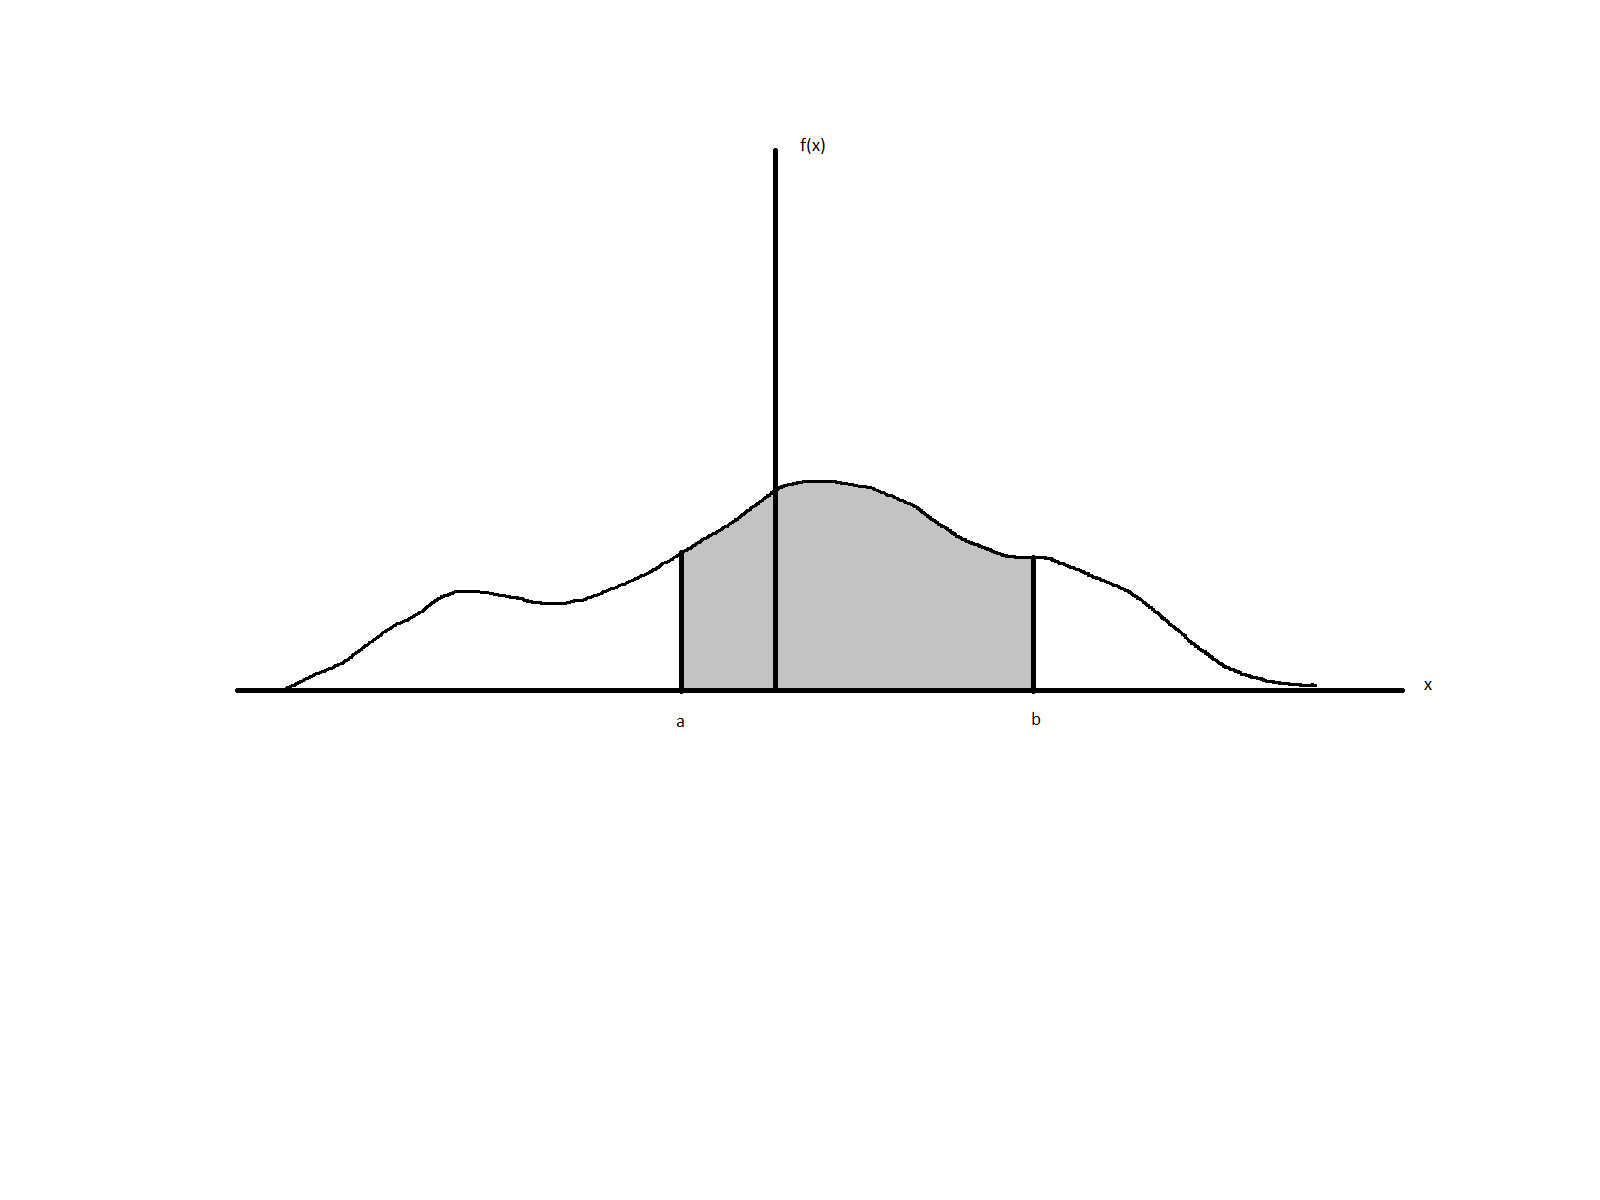
\includegraphics{./images/Less14a.png}
\caption{Figure 3.1a}
\end{figure}

Now using what we now about probability and calculus we know:

\begin{enumerate}
\def\labelenumi{\arabic{enumi}.}
\tightlist
\item
  \(f(x) \geq 0\)
\item
  \(\int_{-\infty}^{\infty}f(x)dx=1\)
\end{enumerate}

Since probabilities are {[}0,1{]}, \(f(x)\) has to be non-negative
otherwise we would get negative probabilities. A common mistake is to
think that \(f(x)\) has to be less than or equal to one. That is not
true. If you are doing this mistake, you are confusing probability with
density. The area under the density curve, which is a probability, has
to be less than or equal to one.

Use calculus knowledge to solve probability problems for continuous
random variables.

For example \(P(X=a)=\int_{a}^{a}f(x)dx=0\).

The cumulative distribution function has the same definition
\[P(X\leq x)=\int_{-\infty}^{x}f(x)dx=F(x)\]

The variable \(x\) in the integral is confusing to students but remember
the variable in the integration is a dummy variable so we could have
written it as\\
\[P(X\leq x)=\int_{-\infty}^{x}f(w)dw=F(x)\]

Using the fundamental theorem of calculus, we know the relationship
between the pdf and cdf

\[f(x)={d \over dx}F(x)\]

Definition 3.1.5 in the book is important if you want to state that two
random variables have the same distribution.

\subsection{Work problem 3.1a including finding
cdf.}\label{work-problem-3.1a-including-finding-cdf.}

Do this by hand. In R you can do the following:

Define the kernel as a vectorized R function

\begin{Shaded}
\begin{Highlighting}[]
\NormalTok{f<-}\ControlFlowTok{function}\NormalTok{(x)\{}
    \KeywordTok{sapply}\NormalTok{(x,(}\ControlFlowTok{function}\NormalTok{(x)((x}\OperatorTok{-}\DecValTok{2}\NormalTok{)}\OperatorTok{*}\NormalTok{(x}\OperatorTok{+}\DecValTok{2}\NormalTok{)}\OperatorTok{*}\NormalTok{\{x}\OperatorTok{>=-}\DecValTok{2}\OperatorTok{&}\NormalTok{x}\OperatorTok{<=}\DecValTok{2}\NormalTok{\})))}
\NormalTok{\}}
\end{Highlighting}
\end{Shaded}

Notice that I used a function inside the function. Since I did not give
it a name it is often called an anonymous function.

A plot of the kernel

\begin{Shaded}
\begin{Highlighting}[]
\KeywordTok{plot}\NormalTok{(}\KeywordTok{seq}\NormalTok{(}\OperatorTok{-}\DecValTok{2}\NormalTok{,}\DecValTok{2}\NormalTok{,.}\DecValTok{01}\NormalTok{),}\KeywordTok{f}\NormalTok{(}\KeywordTok{seq}\NormalTok{(}\OperatorTok{-}\DecValTok{2}\NormalTok{,}\DecValTok{2}\NormalTok{,.}\DecValTok{01}\NormalTok{)),}\DataTypeTok{type=}\StringTok{"l"}\NormalTok{,}\DataTypeTok{ylab=}\StringTok{"f(x)"}\NormalTok{,}\DataTypeTok{xlab=}\StringTok{"x"}\NormalTok{)}
\end{Highlighting}
\end{Shaded}

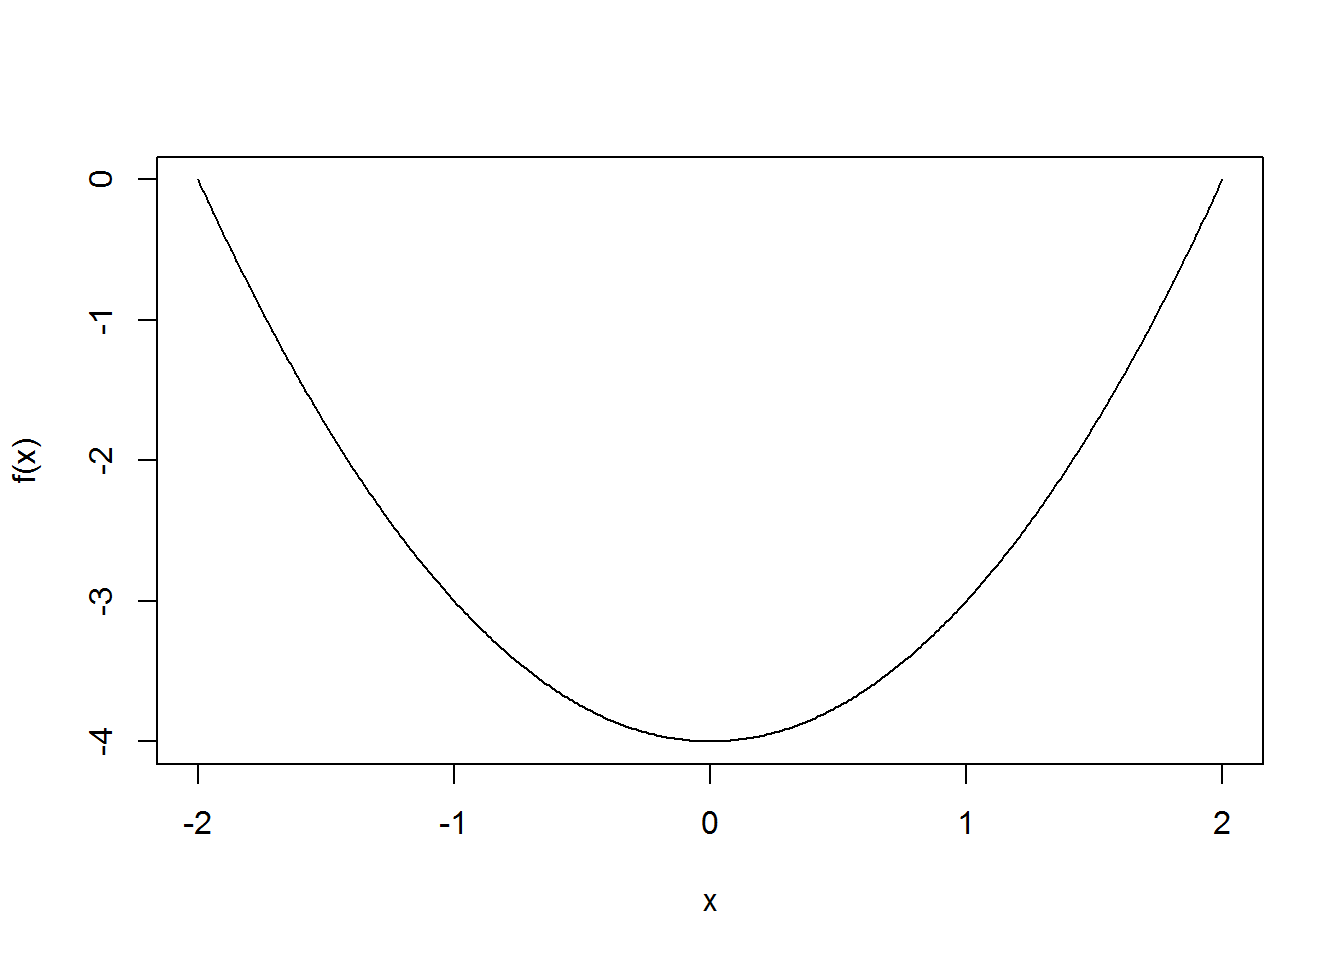
\includegraphics{fastR-Notes_files/figure-latex/unnamed-chunk-150-1.pdf}

Notice this is not a pdf. We must find the scaling constant.

\begin{Shaded}
\begin{Highlighting}[]
\KeywordTok{library}\NormalTok{(MASS)}
\end{Highlighting}
\end{Shaded}

\begin{Shaded}
\begin{Highlighting}[]
\KeywordTok{fractions}\NormalTok{(}\KeywordTok{integrate}\NormalTok{(f,}\OperatorTok{-}\OtherTok{Inf}\NormalTok{,}\OtherTok{Inf}\NormalTok{)}\OperatorTok{$}\NormalTok{value)}
\end{Highlighting}
\end{Shaded}

\begin{verbatim}
## [1] -32/3
\end{verbatim}

Thus the pdf is

\[f(x)={-3 \over 32}(x-2)(x+2) \mbox{ for } -2 \leq x \leq 2\]

and \[f(x)=0 \mbox{ otherwise}\]

Let's see if we need to vectorize the function as the author suggested.
Here is my pdf function

\begin{Shaded}
\begin{Highlighting}[]
\NormalTok{f3.}\DecValTok{1}\NormalTok{<-}\ControlFlowTok{function}\NormalTok{(x)(}\OperatorTok{-}\DecValTok{3}\OperatorTok{/}\DecValTok{32}\OperatorTok{*}\NormalTok{(x}\OperatorTok{-}\DecValTok{2}\NormalTok{)}\OperatorTok{*}\NormalTok{(x}\OperatorTok{+}\DecValTok{2}\NormalTok{)}\OperatorTok{*}\NormalTok{\{x}\OperatorTok{>=-}\DecValTok{2}\OperatorTok{&}\NormalTok{x}\OperatorTok{<=}\DecValTok{2}\NormalTok{\})}
\end{Highlighting}
\end{Shaded}

This would be an R function that started with the letter \texttt{d}.

A plot of the pdf

\begin{Shaded}
\begin{Highlighting}[]
\KeywordTok{plot}\NormalTok{(}\KeywordTok{seq}\NormalTok{(}\OperatorTok{-}\DecValTok{2}\NormalTok{,}\DecValTok{2}\NormalTok{,.}\DecValTok{01}\NormalTok{),}\KeywordTok{f3.1}\NormalTok{(}\KeywordTok{seq}\NormalTok{(}\OperatorTok{-}\DecValTok{2}\NormalTok{,}\DecValTok{2}\NormalTok{,.}\DecValTok{01}\NormalTok{)),}\DataTypeTok{type=}\StringTok{"l"}\NormalTok{,}\DataTypeTok{ylab=}\StringTok{"f(x)"}\NormalTok{,}\DataTypeTok{xlab=}\StringTok{"x"}\NormalTok{)}
\end{Highlighting}
\end{Shaded}

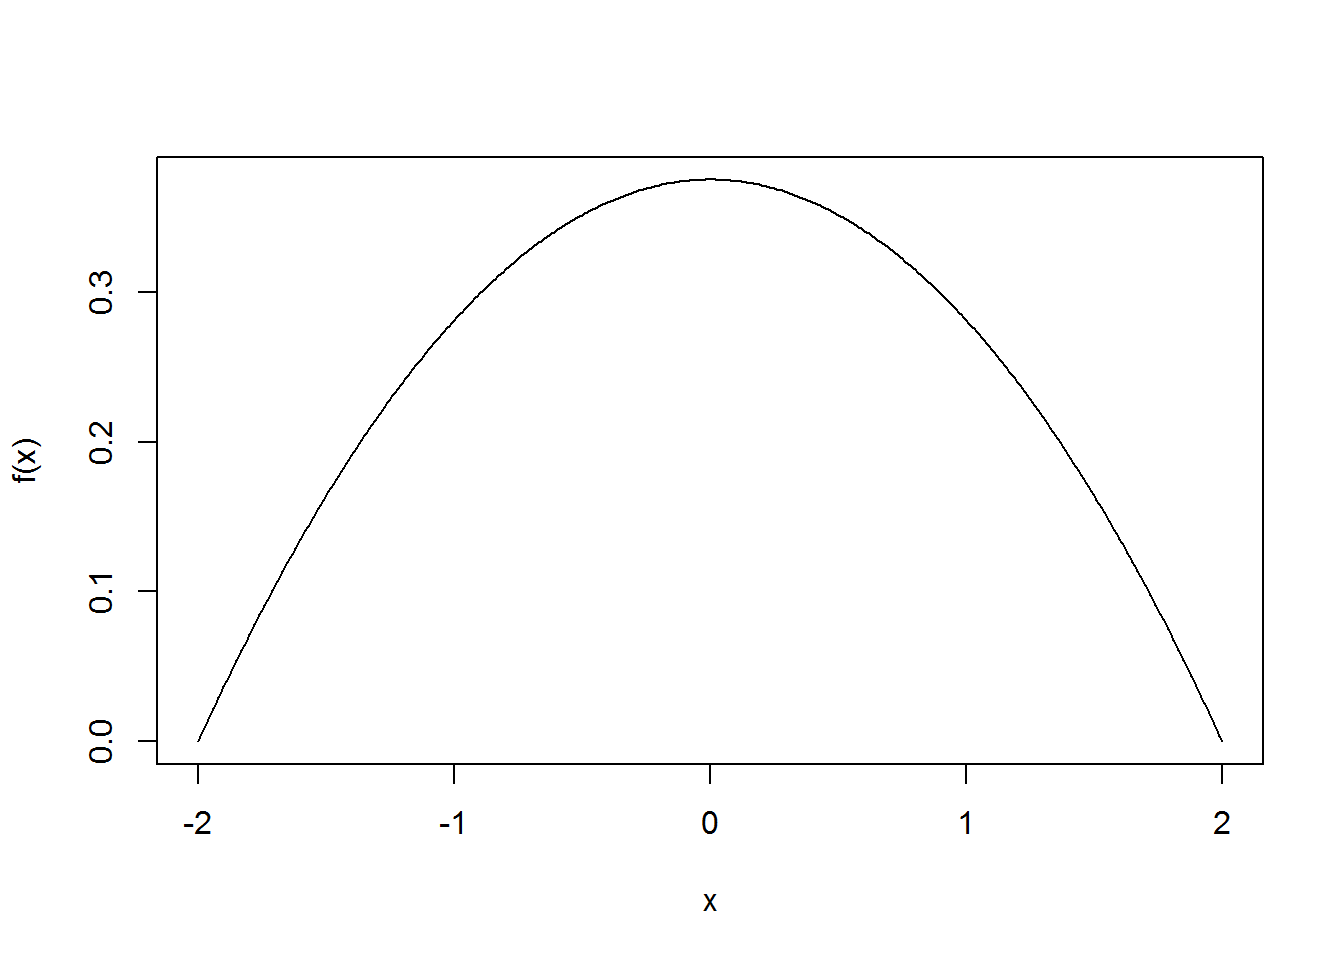
\includegraphics{fastR-Notes_files/figure-latex/unnamed-chunk-154-1.pdf}

This is proper pdf since \[f(x) \geq 0\] and
\[\int_{-\infty}^{\infty}f(x)dx=1\]

\begin{Shaded}
\begin{Highlighting}[]
\KeywordTok{integrate}\NormalTok{(f3.}\DecValTok{1}\NormalTok{,}\OperatorTok{-}\OtherTok{Inf}\NormalTok{,}\OtherTok{Inf}\NormalTok{)}\OperatorTok{$}\NormalTok{value}
\end{Highlighting}
\end{Shaded}

\begin{verbatim}
## [1] 1
\end{verbatim}

It does not appear that we need to vectorize the function. Perhaps the
logical statement is the function that is vectorizing the function for
us.

By hand we get

\[\int_{-\infty}^{\infty}f(x)dx=\int_{-\infty}^{-2}0dx+\int_{-2}^{2}{-3 \over 32}(x-2)(x+2)dx+\int_{2}^{\infty}0dx=\]
\[{-3 \over 32}({x^3 \over 3} -4x) \vert_{-2}^{2}=\]
\[{-3 \over 32}({8 \over 3}-8 -({-8 \over 3} +8) )=\]
\[{-3 \over 32}*(16/3-16)=1\]

The cdf is
\[F(x)=P(X\leq x)=\int_{-\infty}^{x}f(x)dx=\int_{-\infty}^{-2}0dx+\int_{-2}^{x}{-3 \over 32}(x-2)(x+2)dx=\]
\[-{(x^3-12x-16) \over 32}\]

Thus the cdf is \[0 \mbox{ for }x \leq -2\]
\[-{(x^3-12x-16) \over 32} \mbox{ for } -2 \leq x \leq 2\]
\[1 \mbox{ for } x>2\]

As an R function

\begin{Shaded}
\begin{Highlighting}[]
\NormalTok{cdf3.}\DecValTok{1}\NormalTok{<-}\ControlFlowTok{function}\NormalTok{(x)\{}
    \ControlFlowTok{if}\NormalTok{ (x}\OperatorTok{<}\StringTok{ }\OperatorTok{-}\DecValTok{2}\NormalTok{) \{}
\NormalTok{        result=}\DecValTok{0}
\NormalTok{    \} }\ControlFlowTok{else} \ControlFlowTok{if}\NormalTok{ (x}\OperatorTok{>}\DecValTok{2}\NormalTok{)\{}
\NormalTok{        result=}\DecValTok{1}
\NormalTok{    \} }\ControlFlowTok{else}\NormalTok{ result =}\StringTok{ }\OperatorTok{-}\NormalTok{(x}\OperatorTok{^}\DecValTok{3}\OperatorTok{-}\DecValTok{12}\OperatorTok{*}\NormalTok{x}\OperatorTok{-}\DecValTok{16}\NormalTok{)}\OperatorTok{/}\DecValTok{32}
\KeywordTok{return}\NormalTok{(result)}
\NormalTok{\}}
\end{Highlighting}
\end{Shaded}

This would be an R function that started with the letter \texttt{p}.

As a check

\begin{Shaded}
\begin{Highlighting}[]
\KeywordTok{fractions}\NormalTok{(}\KeywordTok{cdf3.1}\NormalTok{(}\OperatorTok{-}\DecValTok{1}\NormalTok{))}
\end{Highlighting}
\end{Shaded}

\begin{verbatim}
## [1] 5/32
\end{verbatim}

\begin{Shaded}
\begin{Highlighting}[]
\KeywordTok{fractions}\NormalTok{(}\KeywordTok{integrate}\NormalTok{(f3.}\DecValTok{1}\NormalTok{,}\OperatorTok{-}\OtherTok{Inf}\NormalTok{,}\OperatorTok{-}\DecValTok{1}\NormalTok{)}\OperatorTok{$}\NormalTok{value)}
\end{Highlighting}
\end{Shaded}

\begin{verbatim}
## [1] 5/32
\end{verbatim}

or equivalently

\begin{Shaded}
\begin{Highlighting}[]
\KeywordTok{fractions}\NormalTok{(}\KeywordTok{integrate}\NormalTok{(f3.}\DecValTok{1}\NormalTok{,}\OperatorTok{-}\DecValTok{2}\NormalTok{,}\OperatorTok{-}\DecValTok{1}\NormalTok{)}\OperatorTok{$}\NormalTok{value)}
\end{Highlighting}
\end{Shaded}

\begin{verbatim}
## [1] 5/32
\end{verbatim}

As an advanced problem, we can create our own \texttt{q} version of the
function as well. This is where we find the quantiles. Here is my code

\begin{Shaded}
\begin{Highlighting}[]
\NormalTok{q3.}\DecValTok{1}\NormalTok{<-}\ControlFlowTok{function}\NormalTok{(y)}\KeywordTok{uniroot}\NormalTok{(}\ControlFlowTok{function}\NormalTok{(x)}\KeywordTok{cdf3.1}\NormalTok{(x)}\OperatorTok{-}\NormalTok{y,}\KeywordTok{c}\NormalTok{(}\OperatorTok{-}\DecValTok{2}\NormalTok{,}\DecValTok{2}\NormalTok{))}\OperatorTok{$}\NormalTok{root}
\end{Highlighting}
\end{Shaded}

I did not put any error checking in this function so I am assuming a
knowledgeable user.

Let's test it.

\begin{Shaded}
\begin{Highlighting}[]
\KeywordTok{q3.1}\NormalTok{(.}\DecValTok{5}\NormalTok{)}
\end{Highlighting}
\end{Shaded}

\begin{verbatim}
## [1] 0
\end{verbatim}

\begin{Shaded}
\begin{Highlighting}[]
\KeywordTok{q3.1}\NormalTok{(.}\DecValTok{75}\NormalTok{)}
\end{Highlighting}
\end{Shaded}

\begin{verbatim}
## [1] 0.6946066
\end{verbatim}

\begin{Shaded}
\begin{Highlighting}[]
\KeywordTok{q3.1}\NormalTok{(}\DecValTok{1}\NormalTok{)}
\end{Highlighting}
\end{Shaded}

\begin{verbatim}
## [1] 2
\end{verbatim}

\begin{Shaded}
\begin{Highlighting}[]
\KeywordTok{q3.1}\NormalTok{(}\DecValTok{0}\NormalTok{)}
\end{Highlighting}
\end{Shaded}

\begin{verbatim}
## [1] -2
\end{verbatim}

Finally, I could write my R function as well.

\begin{Shaded}
\begin{Highlighting}[]
\NormalTok{r3.}\DecValTok{1}\NormalTok{<-}\ControlFlowTok{function}\NormalTok{(n)}\KeywordTok{sapply}\NormalTok{(}\KeywordTok{runif}\NormalTok{(n),q3.}\DecValTok{1}\NormalTok{)}
\end{Highlighting}
\end{Shaded}

This is generating random samples from the distribution.

\begin{Shaded}
\begin{Highlighting}[]
\KeywordTok{set.seed}\NormalTok{(}\DecValTok{2018}\NormalTok{)}
\KeywordTok{r3.1}\NormalTok{(}\DecValTok{40}\NormalTok{)}
\end{Highlighting}
\end{Shaded}

\begin{verbatim}
##  [1] -0.44421232 -0.09678344 -1.40086226 -0.85981410 -0.06853322
##  [6] -0.54394904  0.28665737 -1.09649783  1.50998881  0.12509517
## [11] -0.28019423  0.44615514  1.68262229  0.48473231  0.87117150
## [16]  0.36177270 -0.63245071  0.14131294  0.65832434  0.94636589
## [21] -0.66414309  0.18280379 -1.01699362 -1.23849172  0.73101697
## [26]  0.09591294 -0.46749589  1.32583168  0.26369534 -1.37995268
## [31] -1.05390319  1.06862839 -1.55871257 -0.02612256  0.01648085
## [36]  0.73137964 -1.48148037 -1.44633673  0.21686676 -0.93427163
\end{verbatim}

A plot of the sample is

\begin{Shaded}
\begin{Highlighting}[]
\KeywordTok{library}\NormalTok{(lattice)}
\end{Highlighting}
\end{Shaded}

\begin{Shaded}
\begin{Highlighting}[]
\KeywordTok{set.seed}\NormalTok{(}\DecValTok{2019}\NormalTok{)}
\KeywordTok{densityplot}\NormalTok{(}\KeywordTok{r3.1}\NormalTok{(}\DecValTok{2000}\NormalTok{),}\DataTypeTok{xlab=}\StringTok{"x"}\NormalTok{)}
\end{Highlighting}
\end{Shaded}

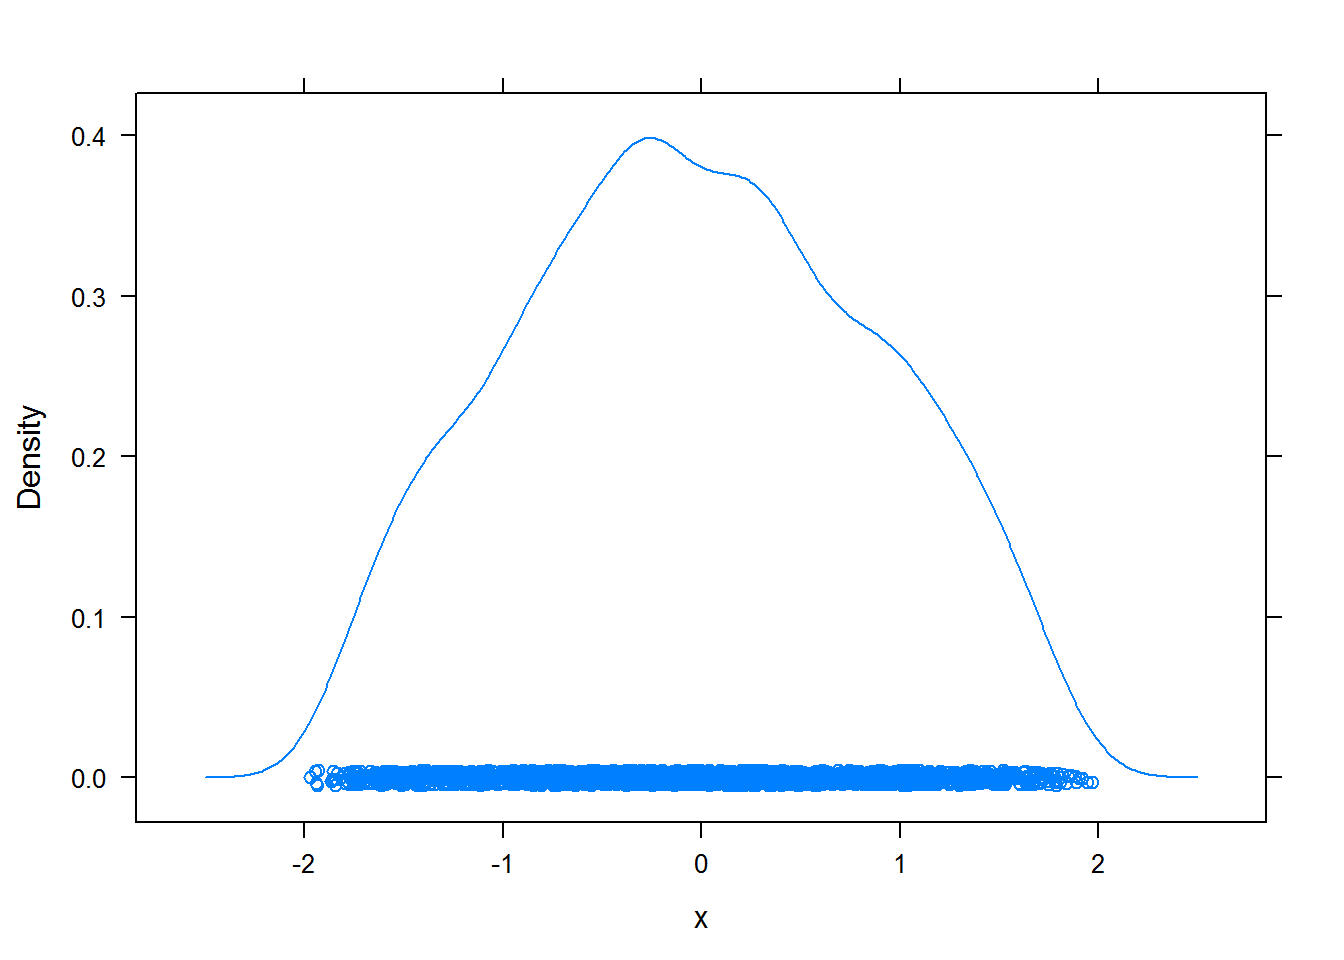
\includegraphics{fastR-Notes_files/figure-latex/unnamed-chunk-165-1.pdf}

This looks like our pdf.

\subsection{Transformation Problem}\label{transformation-problem}

For problem 3.1a, find the pdf of Y where Y=X+2.

Unlike the discrete case, we cannot simply substitute the transformation
relationship into the pdf. However, since equality of distributions
relies on the cdf we will use it.

We want to find the cdf of \(Y\) \[F_{Y}(y)=P(Y \leq y)=\]
\[P(X+2 \leq y)=\] \[P(X \leq y-2)=\] \[F_{X}(y-2)\]

This is the cdf of \(X\) which we know.

Thus the cdf of \(Y\) is \[0 \mbox{ for }y \leq 0\]
\[-{((y-2)^3-12(y-2)-16) \over 32} \mbox{ for } 0 \leq y \leq 4\]
\[1 \mbox{ for } y>4\]

We find the domain of the cdf for \(Y\) by substituting in the domain
values of \(X\) into the transformation relationship.

We have to be careful in this approach that the transformation in
one-to-one and unto. If not, we have to divide the problem into regions
where it is.

The pdf of \(Y\) is found by taking the derivative of the cdf.

\[f_{Y}(y)=-{(3(y-2)^2-12) \over 32} \mbox{ for } 0 \leq y \leq 4\]

We should check that this is a pdf. I will use R to do the work for me.

\begin{Shaded}
\begin{Highlighting}[]
\NormalTok{f3.1a<-}\ControlFlowTok{function}\NormalTok{(y)(}\OperatorTok{-}\DecValTok{3}\OperatorTok{/}\DecValTok{32}\OperatorTok{*}\NormalTok{((y}\OperatorTok{-}\DecValTok{2}\NormalTok{)}\OperatorTok{^}\DecValTok{2}\OperatorTok{-}\DecValTok{4}\NormalTok{)}\OperatorTok{*}\NormalTok{\{y}\OperatorTok{>=}\DecValTok{0}\OperatorTok{&}\NormalTok{y}\OperatorTok{<=}\DecValTok{4}\NormalTok{\})}
\end{Highlighting}
\end{Shaded}

\begin{Shaded}
\begin{Highlighting}[]
\KeywordTok{plot}\NormalTok{(}\KeywordTok{seq}\NormalTok{(}\DecValTok{0}\NormalTok{,}\DecValTok{4}\NormalTok{,.}\DecValTok{01}\NormalTok{),}\KeywordTok{f3.1a}\NormalTok{(}\KeywordTok{seq}\NormalTok{(}\DecValTok{0}\NormalTok{,}\DecValTok{4}\NormalTok{,.}\DecValTok{01}\NormalTok{)),}\DataTypeTok{type=}\StringTok{"l"}\NormalTok{,}\DataTypeTok{ylab=}\StringTok{"f(y)"}\NormalTok{,}\DataTypeTok{xlab=}\StringTok{"y"}\NormalTok{)}
\end{Highlighting}
\end{Shaded}

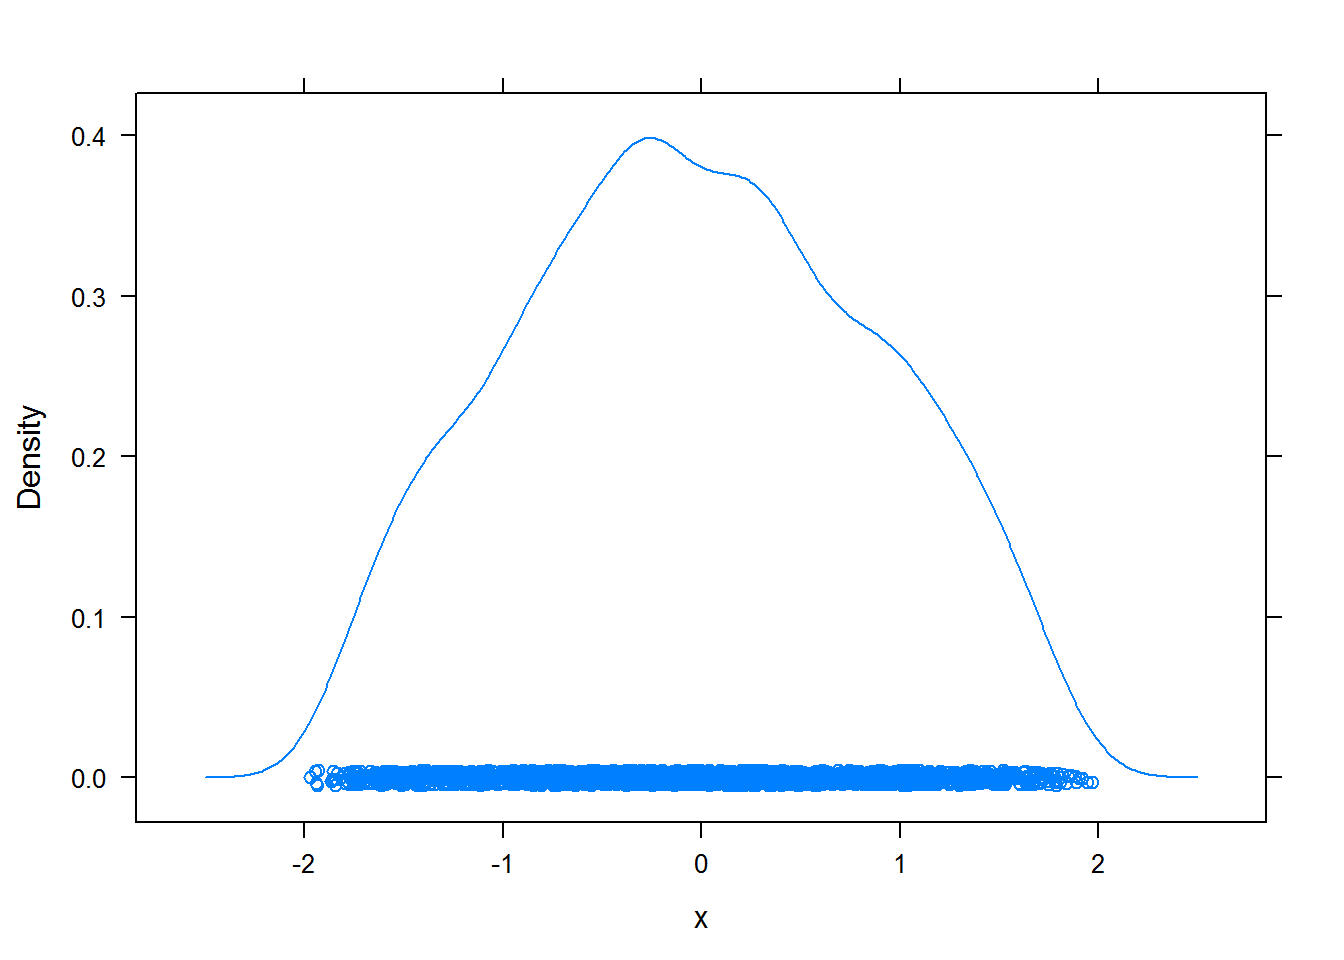
\includegraphics{fastR-Notes_files/figure-latex/unnamed-chunk-167-1.pdf}

\begin{Shaded}
\begin{Highlighting}[]
\KeywordTok{integrate}\NormalTok{(f3.1a,}\DecValTok{0}\NormalTok{,}\DecValTok{4}\NormalTok{)}\OperatorTok{$}\NormalTok{value}
\end{Highlighting}
\end{Shaded}

\begin{verbatim}
## [1] 1
\end{verbatim}

\subsection{Named Continuous Random Variables: Uniform and
Exponential}\label{named-continuous-random-variables-uniform-and-exponential}

We introduce two named distributions, the uniform and exponential.

\subsubsection{Uniform}\label{uniform}

Just as the name implies, for the uniform, the pdf is constant. It is
typically written as \(U(a,b)\). Using the properties of a pdf and the
fact that it must be a constant, the pdf is
\[f(x)={1 \over (b-a)} \mbox{ for } a \leq x \leq b\]

For a \(U(1,1.5)\) what is the pdf? Note that a pdf can be greater than
one.

The pdf is \(f(x)=2\) for \(1 \leq x \leq 1.5\).

Notice that you can use geometry to verify this is a proper pdf.
Likewise, to find the cdf, you can use geometry.

\subsubsection{Exponential}\label{exponential}

Exponential is the interval (time or distance) until next occurrence.
Here the interval is random and the occurrences are fixed, as one. In
the Poisson the occurrences are random and the interval is fixed. The
exponential also uses \(\lambda\) for the parameter but now it has to be
the average number of occurrences per unit time.

Let's work Prob 2.80a again using exponential.

Y = Time in minutes until the next customer arrives. We want
P(Y\textgreater{}20) \(\lambda = 6/60\) which is the average number of
customer per minute.

\begin{Shaded}
\begin{Highlighting}[]
\DecValTok{1}\OperatorTok{-}\KeywordTok{pexp}\NormalTok{(}\DecValTok{20}\NormalTok{,}\DecValTok{1}\OperatorTok{/}\DecValTok{10}\NormalTok{)}
\end{Highlighting}
\end{Shaded}

\begin{verbatim}
## [1] 0.1353353
\end{verbatim}

or using Poisson to check

\begin{Shaded}
\begin{Highlighting}[]
\KeywordTok{dpois}\NormalTok{(}\DecValTok{0}\NormalTok{,}\DecValTok{2}\NormalTok{)}
\end{Highlighting}
\end{Shaded}

\begin{verbatim}
## [1] 0.1353353
\end{verbatim}

The distribution is called exponential because the pdf is an exponential
function, \(f(y)=\lambda e^{-\lambda y}\) for \(y \geq 0\).

The exponential is often used for queuing models. It is also used in
reliability models where we are looking for time to failure. It makes a
strong assumption called the memory-less property. The probability of
failure being greater than time \(t_1 + t_2\) given the item has already
lasted time \(t_1\) is simply the probability an item last more than
time \(t_2\). This is a strong assumption and often not realistic.

\subsection{Additional Homework
Problems}\label{additional-homework-problems}

\begin{enumerate}
\def\labelenumi{\arabic{enumi}.}
\item
  Let the probability density function of \(X\) be exponential with
  \(\lambda = 1\). Find the probability density function of \(Y\) where
  \(y = \sqrt{X}\).
\item
  The average number of cars that enter the North Gate is 48 per hour.
  What is the probability that no cars enter the gate in the next 5
  minutes?
\end{enumerate}

\hypertarget{L13}{\section{Moments}\label{L13}}

\subsection{Objectives}\label{objectives-12}

\begin{enumerate}
\def\labelenumi{\arabic{enumi}.}
\tightlist
\item
  Use Lemma 3.2.2 to find any kth moment about the mean or origin.
\item
  Interpret coefficient of skewness and coefficient of kurtosis.
\end{enumerate}

\subsection{Review}\label{review-1}

Solve problem 2.80a both as a Poisson and an Exponential. Write the
random variable in each case.

\subsubsection{Solution Poisson:}\label{solution-poisson}

X = The number of customers in 20 minutes. We get an average of 6
customers per hour so \(\lambda\) is 2. We want \(P(X=0)\). Using R

\begin{Shaded}
\begin{Highlighting}[]
\KeywordTok{dpois}\NormalTok{(}\DecValTok{0}\NormalTok{,}\DecValTok{2}\NormalTok{)}
\end{Highlighting}
\end{Shaded}

\begin{verbatim}
## [1] 0.1353353
\end{verbatim}

\subsubsection{Solution Exponential:}\label{solution-exponential}

As an exponential, the random variable is Y = the time in minutes until
the next customer arrives. Here the parameter is the average number of
customer per minute, \(\lambda\) =\({1 \over 10}\). The probability
statement is \(P(Y>20)\). using R

\begin{Shaded}
\begin{Highlighting}[]
\DecValTok{1}\OperatorTok{-}\KeywordTok{pexp}\NormalTok{(}\DecValTok{20}\NormalTok{,}\DecValTok{1}\OperatorTok{/}\DecValTok{10}\NormalTok{)}
\end{Highlighting}
\end{Shaded}

\begin{verbatim}
## [1] 0.1353353
\end{verbatim}

Or if you wanted to use W = the time in hours until the next customer
arrives, \(P(W>{1 \over 3})\)

\begin{Shaded}
\begin{Highlighting}[]
\DecValTok{1}\OperatorTok{-}\KeywordTok{pexp}\NormalTok{(}\DecValTok{1}\OperatorTok{/}\DecValTok{3}\NormalTok{,}\DecValTok{6}\NormalTok{)}
\end{Highlighting}
\end{Shaded}

\begin{verbatim}
## [1] 0.1353353
\end{verbatim}

\subsection{Definitions}\label{definitions-2}

\begin{enumerate}
\def\labelenumi{\arabic{enumi}.}
\item
  The notation can be difficult as we now use \(\mu\) to represent
  expected values, which are also called moments. In addition, the prime
  indicates a moment about the mean and the absence of a prime indicates
  a moment about the origin. Note that \(\mu_1\) is sometimes just
  called \(\mu\) and \(\mu_{2}'\) is variance \(\sigma ^2\).
\item
  Lemma 3.2.2 is the key basic idea.
\end{enumerate}

\[E[t(X)]=\int_{-\infty}^{\infty}t(x)f(x)dx\]

\begin{enumerate}
\def\labelenumi{\arabic{enumi}.}
\setcounter{enumi}{2}
\item
  Moments about the origin:
  \[\mu_{k}=E(X^k)=\int_{-\infty}^{\infty}x^k f(x)dx\]
\item
  Moments about the mean:
  \[\mu_{k}'=E[(X-E(X))^k]=\int_{-\infty}^{\infty}(x-\mu)^k f(x)dx\]
\item
  Practical: Moments are used to summarize/describe the data. The first
  moment about the origin is the mean and describes location. The second
  moment about the mean is variance and describes spread of the
  distribution. The third moment about the mean is used to calculate the
  coefficient of skewness which describes symmetry of the distribution.
  Finally, the fourth moment about the mean can be used to calculate the
  coefficient of kurtosis which describes if the data has a peak.
\end{enumerate}

\subsection{Practice}\label{practice-1}

For X \textasciitilde{} U(0,2), find
\(E(X),E(X^2)\),\(V(X)\),\(E(X^3)\),\(\mu^{'}_3\), and \(\gamma_1\).

The pdf is \(f(x)={1 \over 2}\) for \(0\leq x \leq 2\).

\[E(X)=\int_{-\infty}^{\infty}xf(x)dx=\int_{0}^{2}{1 \over 2}xdx={x^2 \over 4}\vert_{0}^{2}=1\]
\[E(X^2)=\int_{-\infty}^{\infty}x^2f(x)dx=\int_{0}^{2}{1 \over 2}x^2dx={x^3 \over 6}\vert_{0}^{2}={4 \over 3}\]
Check using R

\begin{Shaded}
\begin{Highlighting}[]
\KeywordTok{library}\NormalTok{(MASS)}
\end{Highlighting}
\end{Shaded}

\begin{Shaded}
\begin{Highlighting}[]
\KeywordTok{fractions}\NormalTok{(}\KeywordTok{integrate}\NormalTok{(}\ControlFlowTok{function}\NormalTok{(x)}\DecValTok{1}\OperatorTok{/}\DecValTok{2}\OperatorTok{*}\NormalTok{x}\OperatorTok{*}\NormalTok{(x}\OperatorTok{>=}\DecValTok{0} \OperatorTok{&}\StringTok{ }\NormalTok{x}\OperatorTok{<=}\DecValTok{2}\NormalTok{),}\DecValTok{0}\NormalTok{,}\DecValTok{2}\NormalTok{)}\OperatorTok{$}\NormalTok{value)}
\end{Highlighting}
\end{Shaded}

\begin{verbatim}
## [1] 1
\end{verbatim}

\begin{Shaded}
\begin{Highlighting}[]
\KeywordTok{fractions}\NormalTok{(}\KeywordTok{integrate}\NormalTok{(}\ControlFlowTok{function}\NormalTok{(x)}\DecValTok{1}\OperatorTok{/}\DecValTok{2}\OperatorTok{*}\NormalTok{x}\OperatorTok{^}\DecValTok{2}\OperatorTok{*}\NormalTok{(x}\OperatorTok{>=}\DecValTok{0} \OperatorTok{&}\StringTok{ }\NormalTok{x}\OperatorTok{<=}\DecValTok{2}\NormalTok{),}\DecValTok{0}\NormalTok{,}\DecValTok{2}\NormalTok{)}\OperatorTok{$}\NormalTok{value)}
\end{Highlighting}
\end{Shaded}

\begin{verbatim}
## [1] 4/3
\end{verbatim}

\[V(X)=E[(X-\mu)^2]=E(X^2)-E(X)^2={4 \over 3}-1^2={1 \over 3}\]

\begin{Shaded}
\begin{Highlighting}[]
\KeywordTok{fractions}\NormalTok{(}\KeywordTok{integrate}\NormalTok{(}\ControlFlowTok{function}\NormalTok{(x)}\DecValTok{1}\OperatorTok{/}\DecValTok{2}\OperatorTok{*}\NormalTok{(x}\OperatorTok{-}\DecValTok{1}\NormalTok{)}\OperatorTok{^}\DecValTok{2}\OperatorTok{*}\NormalTok{(x}\OperatorTok{>=}\DecValTok{0} \OperatorTok{&}\StringTok{ }\NormalTok{x}\OperatorTok{<=}\DecValTok{2}\NormalTok{),}\DecValTok{0}\NormalTok{,}\DecValTok{2}\NormalTok{)}\OperatorTok{$}\NormalTok{value)}
\end{Highlighting}
\end{Shaded}

\begin{verbatim}
## [1] 1/3
\end{verbatim}

\[E(X^3)=\int_{-\infty}^{\infty}x^3f(x)dx=\int_{0}^{2}{1 \over 2}x^3dx={x^4 \over 8}\vert_{0}^{2}=2\]

\begin{Shaded}
\begin{Highlighting}[]
\KeywordTok{fractions}\NormalTok{(}\KeywordTok{integrate}\NormalTok{(}\ControlFlowTok{function}\NormalTok{(x)}\DecValTok{1}\OperatorTok{/}\DecValTok{2}\OperatorTok{*}\NormalTok{x}\OperatorTok{^}\DecValTok{3}\OperatorTok{*}\NormalTok{(x}\OperatorTok{>=}\DecValTok{0} \OperatorTok{&}\StringTok{ }\NormalTok{x}\OperatorTok{<=}\DecValTok{2}\NormalTok{),}\DecValTok{0}\NormalTok{,}\DecValTok{2}\NormalTok{)}\OperatorTok{$}\NormalTok{value)}
\end{Highlighting}
\end{Shaded}

\begin{verbatim}
## [1] 2
\end{verbatim}

\[\mu^{'}_3=E[(X-\mu)^3]=\int_{-\infty}^{\infty}(x-1)^3f(x)dx=\int_{0}^{2}{1 \over 2}(x-1)^3dx\]

This is going to be difficult but can be done if we expand the
polynomial. We could use R.

\begin{Shaded}
\begin{Highlighting}[]
\KeywordTok{fractions}\NormalTok{(}\KeywordTok{integrate}\NormalTok{(}\ControlFlowTok{function}\NormalTok{(x)}\DecValTok{1}\OperatorTok{/}\DecValTok{2}\OperatorTok{*}\NormalTok{(x}\OperatorTok{-}\DecValTok{1}\NormalTok{)}\OperatorTok{^}\DecValTok{3}\OperatorTok{*}\NormalTok{(x}\OperatorTok{>=}\DecValTok{0} \OperatorTok{&}\StringTok{ }\NormalTok{x}\OperatorTok{<=}\DecValTok{2}\NormalTok{),}\DecValTok{0}\NormalTok{,}\DecValTok{2}\NormalTok{)}\OperatorTok{$}\NormalTok{value)}
\end{Highlighting}
\end{Shaded}

\begin{verbatim}
## [1] 0
\end{verbatim}

We could also use Lemma 3.3.2.
\[\mu_{3}'=\mu_{3}-3\mu_{2}\mu+2\mu^3=2-3*{4 \over 3}*1+2*1^3=2-4+2=0\]

\[\gamma_1={\mu_{3}' \over \sigma^3}={0 \over \sigma^3}=0\]

It is a symmetric distribution.

Do Homework 3.12

\hypertarget{L14}{\section{Generating Functions}\label{L14}}

\subsection{Objectives}\label{objectives-13}

\begin{enumerate}
\def\labelenumi{\arabic{enumi}.}
\tightlist
\item
  Given a pdf/pmf find the mgf, \(M_{X}(t)\).
\item
  Find moments from a moment generating function.
\item
  Use moment generating function to find distributions of a
  transformation of a random variable, Thm 3.3.6.
\end{enumerate}

\subsection{Review}\label{review-2}

The Maclaurin series is a special case of the Taylor series. This is a
power series representation of a function. We now have a fourth way to
represent a function. One is a table, another is a formula, another is a
graph, and now we can use an infinite sum. In general the Maclaurin
series is

\[f(x)=f(0)+{f'(0)x \over 1!}+{f''(0)x^2 \over 2!}+{f^{(3)}(0)x^3 \over 3!}+\dots+{f^{(k)}(0)x^k \over k!}+\dots\]

In Calculus we were interested in using the power series to represent
function and one of the most common was

\[e^x=1+x+{x^2 \over 2!}+{x^3 \over 3!}+\dots\]

We will use this expression.

Also remember that moments characterize a distribution. However, to find
them we need to integrate. From last lesson we have

\[\mu_{k}=E(X^k)=\int_{-\infty}^{\infty}x^k f(x)dx\]

The key idea in this lesson is that we want to find a single function
that summarizes, generates, all the moments of a distribution. Sounds
like a crazy idea, but in fact it can be done. It is called the moment
generating function. There are two advantages of the moment generating
functions

\texttt{i)} You use derivatives instead of integration to find moments,
differentiation is often much easier than integration.

\texttt{ii)} If you can recognize a moment generating function, a big
if, then you can find the distribution of a linear transformation of a
random variable or the linear combination of random variables. This is
often easier than using the cdf method we learned earlier.

\subsection{Moment Generating
Functions}\label{moment-generating-functions}

By definition the moment generating function is:

\[M_{X}(t)=E[e^{tX}] = \int_{-\infty}^{\infty}e^{tx}f(x)dx\] for
continuous random variables; for discrete random variables, replace the
integration with a summation.

To find a the kth moment about the origin take the kth derivative of the
moment generating function and evaluate at t = 0. That is
\[\mu_{k}=\left(  {d^{k}M_{X}(t) \over dt^{k}} \right) _{t=0}\]

Why would this work? The book gives a nice summary of the ideas. Along a
similar thread, let's use the Maclaurin power series of \(e^tx\):

\[e^{tx}=1+tx+t^{2}x^{2}/2! + \dots \]

Thus

\[M_{X}(t)=E[e^{tX}]=E[1+tx+t^{2}x^{2}/2! + \dots]=1+tE[X]+t^{2}E[X^{2}]+\dots\]

Now taking the derivative with respect to \(t\) and then evaluating at
\(t=0\) leads to the kth moment about the origin.

\subsection{Practice}\label{practice-2}

\begin{enumerate}
\def\labelenumi{\arabic{enumi}.}
\tightlist
\item
  Find the moment generating function for \(U(0,1)\).
\end{enumerate}

\[E(e^{tX})=\int_{-\infty}^{\infty}e^{tx}f(x)dx=\int_{0}^{1}e^{tx}dx=={1 \over t}e^{tx}\vert_{0}^{1}={1 \over t}\left[e^{t}-1\right]\]

Note that this function is not defined at \(t=0\) but we can use our
Macluarin again to help us.

\[M_{X}(t)={1 \over t}\left[e^{t}-1\right]={1 \over t}\left[t+{t^2 \over 2!}+\dots \right]=\left[1+{t \over 2!}+{t^2 \over 3!}+\dots \right]\]

Now you can take the derivative and evaluate at \(t=0\).

\[{dM_{X}(t) \over dt}_{t=0}={1 \over 2}\]

\begin{enumerate}
\def\labelenumi{\arabic{enumi}.}
\setcounter{enumi}{1}
\tightlist
\item
  The moment generating function for the Poisson is
  \(e^{-\lambda + \lambda e^{t}}\), find the mean and variance.
\end{enumerate}

\[{dM_{X}(t) \over dt}=\left(e^{-\lambda + \lambda e^{t}}\right) \lambda e^{t}\]

Evaluating at \(t=0\) yields
\[E(X)=\left(e^{-\lambda + \lambda e^{0}}\right) \lambda e^{0}=\left(e^{-\lambda + \lambda} \right) \lambda=\lambda\]

\[E(X^2)=\mu_{2}=\left(  {d^{2}M_{X}(t) \over dt^{2}} \right) _{t=0}\]

\[{d^{2}M_{X}(t) \over dt^{2}}=\left(e^{-\lambda + \lambda e^{t}}\right) \lambda + \left(e^{-\lambda + \lambda e^{t}}\right) \lambda^2 e^{2t}\]

\[\left(  {d^{2}M_{X}(t) \over dt^{2}} \right) _{t=0}=\left(e^{-\lambda + \lambda e^{0}}\right) \lambda + \left(e^{-\lambda + \lambda e^{0}}\right) \lambda^2 e^{0}=\lambda +\lambda^2\]

Finally,

\[V(X)=E(X^2)-E(X)=\lambda +\lambda^2-(\lambda)^2=\lambda\]

\subsection{Transformations}\label{transformations}

There is no need to memorize the formulas in Theorem 3.3.6, you can
derive them. For example, let \(Y=aX\)

\[M_{Y}(t)=E(e^{tY})=E(e^{(ta)X)})=M_{X}(at)\]

The problem with this method is that we have to recognize the moment
generating function. This is not necessarily easy.

\subsection{Practice}\label{practice-3}

Given \(X\sim U(0,1)\) find \(Y=2X+3\) using Thm 3.3.6 and then the cdf
method.

\[M_{X}(t)={1 \over t}\left[e^{t}-1\right]\]
\[M_{Y}(t)=E(e^{tY})=E(e^{t(2X+3)})=E(e^{2tx}e^{3t})=e^{3t}E(e^{2tX})=e^{3t}M_{X}(2t)=\]
\[e^{3t}{1 \over 2t}\left[e^{2t}-1\right] = {1 \over 2t}\left[e^{5t}-e^{3t}\right]\]

Now we know \[M_{Y}(t)={1 \over 2t}\left[e^{5t}-e^{3t}\right]\] but the
difficult part is that we have to recognize this. It turns out, if you
look at the table in the back of the book, this is a uniform. Thus
\[Y \sim U(3,5)\]

Using the cdf method \[X \sim U(0,1)\] \[f(x)=1\] \[Y=2X+3\]

\[F_{Y}(y)=P(Y \leq y)=P(2X+3 \leq y)=P\left( X \leq {y-3 \over 2}\right) =\]
\[\int_{0}^{{y-3 \over 2}}1dx={y-3 \over 2}\]
\[f_{Y}(y)={dF_{Y}(y) \over dy}={1 \over 2} \mbox{ for } 0 \leq {y-3 \over 2} \leq 1\]
Cleaning this up \[f_{Y}(y)={1 \over 2} \mbox{ for } 3 \leq y \leq 5\]

This is a uniform.

\hypertarget{L15}{\section{Important Continous
Distributions}\label{L15}}

\subsection{Objectives}\label{objectives-14}

\begin{enumerate}
\def\labelenumi{\arabic{enumi}.}
\tightlist
\item
  Solve probability problems involving the normal, gamma, Weibull, and
  beta distributions.
\item
  Find distribution or mgf for transformations of known distributions.
\item
  Find quantiles of distributions.
\end{enumerate}

\subsection{Normal}\label{normal}

Normal arises from the sum of random variables, common when errors are
additive. The reading on this section is good, it brings in many ideas
from previous sections and motivates why the standard normal is
important.

The empirical rule is used for the normal. 68\% of population within one
standard deviation of the mean, 95\% within 2, and 99.7 within 3. This
is the idea behind the six sigma movement.

The normal has two parameters, the mean and the standard deviation. They
completely specify the distribution. The notation is
\[X \sim N(\mu,\sigma)\]

The pdf for a normal is difficult to integrate and there is no closed
form solution for the cdf. Software packages use a numerical method to
find the cdf.

A common distribution is the standard normal
\(Z={x - \mu \over \sigma}\) where \(X \sim N(\mu,\sigma)\)

We can check these in R. Using a standard normal, the default in R

\begin{Shaded}
\begin{Highlighting}[]
\KeywordTok{qnorm}\NormalTok{(.}\DecValTok{68}\OperatorTok{+}\NormalTok{.}\DecValTok{16}\NormalTok{)}
\end{Highlighting}
\end{Shaded}

\begin{verbatim}
## [1] 0.9944579
\end{verbatim}

\begin{Shaded}
\begin{Highlighting}[]
\KeywordTok{qnorm}\NormalTok{(.}\DecValTok{16}\NormalTok{)}
\end{Highlighting}
\end{Shaded}

\begin{verbatim}
## [1] -0.9944579
\end{verbatim}

So 68\% is between -1 and 1, which is within one standard deviation of
the mean. Or using pnorm

\begin{Shaded}
\begin{Highlighting}[]
\KeywordTok{pnorm}\NormalTok{(}\DecValTok{1}\NormalTok{)}\OperatorTok{-}\KeywordTok{pnorm}\NormalTok{(}\OperatorTok{-}\DecValTok{1}\NormalTok{)}
\end{Highlighting}
\end{Shaded}

\begin{verbatim}
## [1] 0.6826895
\end{verbatim}

Just to check, let's use a different Normal with \(\mu\) 4 and
\(\sigma\) of 3.

\begin{Shaded}
\begin{Highlighting}[]
\KeywordTok{pnorm}\NormalTok{(}\DecValTok{7}\NormalTok{,}\DecValTok{4}\NormalTok{,}\DecValTok{3}\NormalTok{)}\OperatorTok{-}\KeywordTok{pnorm}\NormalTok{(}\DecValTok{1}\NormalTok{,}\DecValTok{4}\NormalTok{,}\DecValTok{3}\NormalTok{)}
\end{Highlighting}
\end{Shaded}

\begin{verbatim}
## [1] 0.6826895
\end{verbatim}

Likewise for two and three standard deviations

\begin{Shaded}
\begin{Highlighting}[]
\KeywordTok{pnorm}\NormalTok{(}\DecValTok{2}\NormalTok{)}\OperatorTok{-}\KeywordTok{pnorm}\NormalTok{(}\OperatorTok{-}\DecValTok{2}\NormalTok{)}
\end{Highlighting}
\end{Shaded}

\begin{verbatim}
## [1] 0.9544997
\end{verbatim}

\begin{Shaded}
\begin{Highlighting}[]
\KeywordTok{pnorm}\NormalTok{(}\DecValTok{3}\NormalTok{)}\OperatorTok{-}\KeywordTok{pnorm}\NormalTok{(}\OperatorTok{-}\DecValTok{3}\NormalTok{)}
\end{Highlighting}
\end{Shaded}

\begin{verbatim}
## [1] 0.9973002
\end{verbatim}

The normal will place an important role in hypothesis testing because of
the Central Limit Theorem.

To bring some other ideas back in. The book claims that the moment
generating function for \(N(\mu,\sigma)\) is
\[M_{X}(t)=e^{\mu t + {\sigma ^2 t^2 \over 2}}\]

We can go from any Normal to the standard Normal using the following
transformation, Z is used for the standard normal:
\[Z={X - \mu \over \sigma}\]

We know \(E(X)=\mu\) so
\(E(Z)=E\left( {X - \mu \over \sigma} \right)={1\over \sigma}E(x-\mu)={1\over \sigma}(E(x)-\mu)=0\)

To find the distribution of \(Z\) use the cdf method or the mgf method.
We will use that later.

\[M_{Z}(t)=E(e^{Zt})=E\left[e^{\left( {X - \mu \over \sigma}t \right)} \right] = \]
\[e^{-{\mu \over \sigma}t}E\left[e^{\left( {X  \over \sigma}t \right)} \right] = \]
\[e^{-{\mu \over \sigma}t}M_{X}\left( {t  \over \sigma}\right)=\]
\[e^{-{\mu \over \sigma}t}\left[e^{\mu {t \over \sigma} + {\sigma ^2 t^2 \over \sigma^2 2}}\right]=e^{-{t^2 \over 2}}\]

Now we must recognize this moment generating function, which is the
Normal with \(\mu =\) 0 and \(\sigma =\) 1.

For a standard Normal, find \(E(X^2)\).

\[{d^2M(t) \over dt^2}\vert_{t=0}=\left(e^{-{t^2 \over 2}}+\left(e^{-{t^2 \over 2}}\right) t^2 \right)\vert_{t=0}=1\]

\subsection{Gamma}\label{gamma}

The gamma distribution is for non-negative random variables. It is an
extremely flexible distribution. It has been used in reliability
analysis as well as medical fields for survival analysis. The gamma
distribution has two parameters \(\alpha\) called the shape parameter
and \(\lambda\) called the rate. If \(\alpha\) is an integer then the
gamma is a generalization of the exponential and can represent the time
until \(\alpha\) occurrences. You can give R rate for the parameter or
1/rate, called scale, be careful. Look at the help menu.

The pdf has a gamma function in for the scaling constant. This function
is implemented in R.

\begin{Shaded}
\begin{Highlighting}[]
\KeywordTok{gamma}\NormalTok{(}\DecValTok{4}\NormalTok{)}
\end{Highlighting}
\end{Shaded}

\begin{verbatim}
## [1] 6
\end{verbatim}

\begin{Shaded}
\begin{Highlighting}[]
\KeywordTok{gamma}\NormalTok{(.}\DecValTok{5}\NormalTok{)}
\end{Highlighting}
\end{Shaded}

\begin{verbatim}
## [1] 1.772454
\end{verbatim}

\subsection{Weibull}\label{weibull}

This distributions is also used to model failures where the entire
system fails when the weakest link breaks. The Weibull has two
parameters, \(\alpha\) the shape parameter, and \(\beta\) the scale
parameter.

\subsection{Beta}\label{beta}

The Beta generalizes the uniform and is used to model proportions. The
beta distribution also has two parameters \(\alpha\) and \(\beta\). The
bottom of page 143 has a nice summary of the impact of \(\alpha\) and
\(\beta\) on the shape of the distribution.

Note: Read the last three paragraphs on page 144.

\subsection{Problems}\label{problems-1}

\begin{enumerate}
\def\labelenumi{\arabic{enumi})}
\tightlist
\item
  The scores on an exam can be model as a normal with mean 75 and
  variance 100.
\end{enumerate}

\begin{enumerate}
\def\labelenumi{\alph{enumi})}
\tightlist
\item
  Find the probability of scoring more than 90.
\item
  Find the .8-quantile
\item
  Given that someone scored more than 50, what is the probability of
  scoring less than 90?
\end{enumerate}

\begin{Shaded}
\begin{Highlighting}[]
\DecValTok{1}\OperatorTok{-}\KeywordTok{pnorm}\NormalTok{(}\DecValTok{90}\NormalTok{,}\DecValTok{75}\NormalTok{,}\DecValTok{10}\NormalTok{)}
\end{Highlighting}
\end{Shaded}

\begin{verbatim}
## [1] 0.0668072
\end{verbatim}

\begin{Shaded}
\begin{Highlighting}[]
\KeywordTok{qnorm}\NormalTok{(.}\DecValTok{8}\NormalTok{,}\DecValTok{75}\NormalTok{,}\DecValTok{10}\NormalTok{)}
\end{Highlighting}
\end{Shaded}

\begin{verbatim}
## [1] 83.41621
\end{verbatim}

\begin{Shaded}
\begin{Highlighting}[]
\NormalTok{(}\KeywordTok{pnorm}\NormalTok{(}\DecValTok{90}\NormalTok{,}\DecValTok{75}\NormalTok{,}\DecValTok{10}\NormalTok{)}\OperatorTok{-}\KeywordTok{pnorm}\NormalTok{(}\DecValTok{50}\NormalTok{,}\DecValTok{75}\NormalTok{,}\DecValTok{10}\NormalTok{))}\OperatorTok{/}\NormalTok{(}\DecValTok{1}\OperatorTok{-}\KeywordTok{pnorm}\NormalTok{(}\DecValTok{50}\NormalTok{,}\DecValTok{75}\NormalTok{,}\DecValTok{10}\NormalTok{))}
\end{Highlighting}
\end{Shaded}

\begin{verbatim}
## [1] 0.9327754
\end{verbatim}

\begin{enumerate}
\def\labelenumi{\arabic{enumi})}
\setcounter{enumi}{1}
\tightlist
\item
  The percentages on an exam can be modeled with a Beta distribution
  with \(\alpha = 5\) and \(\beta = 2.7\). Here is a plot of the pdf.
\end{enumerate}

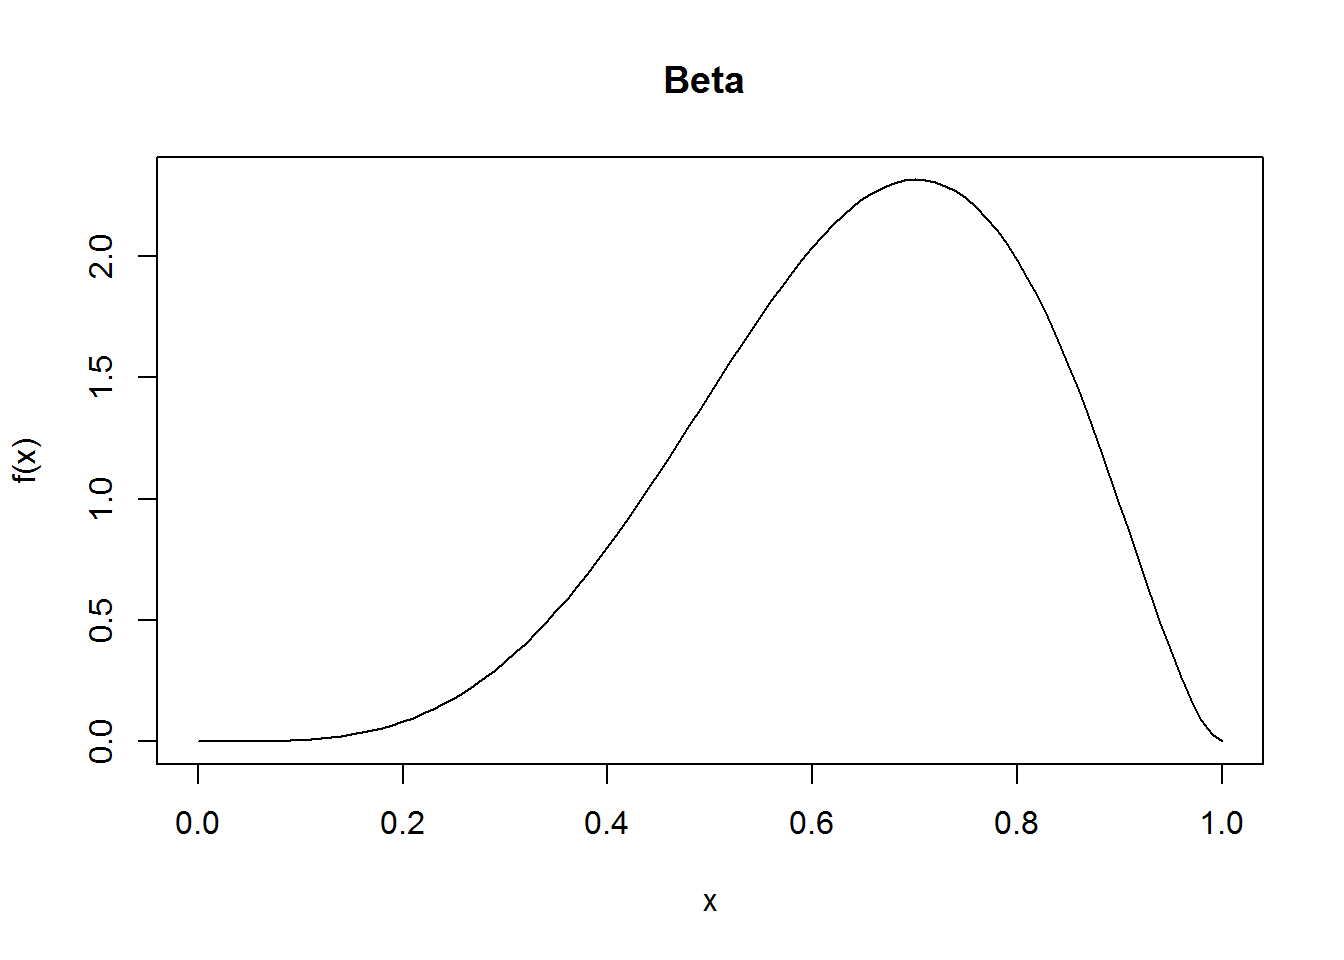
\includegraphics{fastR-Notes_files/figure-latex/unnamed-chunk-186-1.pdf}

\begin{enumerate}
\def\labelenumi{\alph{enumi})}
\tightlist
\item
  Find the probability of scoring more than .90.
\item
  Find the .8-quantile
\item
  Given that someone scored more than .50, what is the probability of
  scoring less than .90?
\end{enumerate}

\begin{Shaded}
\begin{Highlighting}[]
\DecValTok{1}\OperatorTok{-}\KeywordTok{pbeta}\NormalTok{(}\FloatTok{0.9}\NormalTok{,}\DecValTok{5}\NormalTok{,}\FloatTok{2.7}\NormalTok{)}
\end{Highlighting}
\end{Shaded}

\begin{verbatim}
## [1] 0.04089716
\end{verbatim}

\begin{Shaded}
\begin{Highlighting}[]
\KeywordTok{qbeta}\NormalTok{(.}\DecValTok{8}\NormalTok{,}\DecValTok{5}\NormalTok{,}\FloatTok{2.7}\NormalTok{)}
\end{Highlighting}
\end{Shaded}

\begin{verbatim}
## [1] 0.7967842
\end{verbatim}

\begin{Shaded}
\begin{Highlighting}[]
\NormalTok{(}\KeywordTok{pbeta}\NormalTok{(.}\DecValTok{9}\NormalTok{,}\DecValTok{5}\NormalTok{,}\FloatTok{2.7}\NormalTok{)}\OperatorTok{-}\KeywordTok{pbeta}\NormalTok{(.}\DecValTok{5}\NormalTok{,}\DecValTok{5}\NormalTok{,}\FloatTok{2.7}\NormalTok{))}\OperatorTok{/}\NormalTok{(}\DecValTok{1}\OperatorTok{-}\KeywordTok{pbeta}\NormalTok{(.}\DecValTok{5}\NormalTok{,}\DecValTok{5}\NormalTok{,}\FloatTok{2.7}\NormalTok{))}
\end{Highlighting}
\end{Shaded}

\begin{verbatim}
## [1] 0.9496102
\end{verbatim}

\begin{enumerate}
\def\labelenumi{\arabic{enumi})}
\setcounter{enumi}{2}
\tightlist
\item
  The arrival of customers at a restaurant follows a Poison process with
  15 customers per hour on average.
\end{enumerate}

\begin{enumerate}
\def\labelenumi{\alph{enumi})}
\tightlist
\item
  Using a Poisson random variable, find the probability of 2 or less
  customers in 15 minutes.
\item
  Same probability question as part a, but using a Gamma with the random
  variable as time in minutes until 3 customers arrive.
\end{enumerate}

\begin{Shaded}
\begin{Highlighting}[]
\KeywordTok{ppois}\NormalTok{(}\DecValTok{2}\NormalTok{,}\DecValTok{15}\OperatorTok{/}\DecValTok{4}\NormalTok{)}
\end{Highlighting}
\end{Shaded}

\begin{verbatim}
## [1] 0.2770684
\end{verbatim}

\begin{Shaded}
\begin{Highlighting}[]
\DecValTok{1}\OperatorTok{-}\KeywordTok{pgamma}\NormalTok{(}\DecValTok{15}\NormalTok{,}\DecValTok{3}\NormalTok{,}\DecValTok{1}\OperatorTok{/}\DecValTok{4}\NormalTok{)}
\end{Highlighting}
\end{Shaded}

\begin{verbatim}
## [1] 0.2770684
\end{verbatim}

\begin{Shaded}
\begin{Highlighting}[]
\DecValTok{1}\OperatorTok{-}\KeywordTok{pgamma}\NormalTok{(}\DecValTok{15}\NormalTok{,}\DecValTok{3}\NormalTok{,}\DataTypeTok{scale=}\DecValTok{4}\NormalTok{)}
\end{Highlighting}
\end{Shaded}

\begin{verbatim}
## [1] 0.2770684
\end{verbatim}

\hypertarget{L16}{\section{Plots of Distributions}\label{L16}}

\subsection{Objectives}\label{objectives-15}

\begin{enumerate}
\def\labelenumi{\arabic{enumi}.}
\tightlist
\item
  Interpret normal-quantile plots and explain the types of departures
  from normality.\\
\item
  Generate quantile-quantile plots for any distribution.\\
\item
  Given data, generate density plots in R.
\end{enumerate}

\subsection{Review}\label{review-3}

The time to failure of an anchor chain in years in follows a Weibull
distribution with shape parameter 2 and scale parameter 10. What is the
third quartile?

\begin{Shaded}
\begin{Highlighting}[]
\KeywordTok{qweibull}\NormalTok{(.}\DecValTok{75}\NormalTok{,}\DecValTok{2}\NormalTok{,}\DecValTok{10}\NormalTok{)}
\end{Highlighting}
\end{Shaded}

\begin{verbatim}
## [1] 11.7741
\end{verbatim}

\subsection{Background}\label{background-1}

When we have data how do we estimate the pdf and/or determine if one of
our known distributions is appropriate to use as a model? This is an
empirical study question and can never be answered in certainty. This is
the work of analysts and is difficult and a bit of an art.

\subsection{Density Estimation}\label{density-estimation}

First, we will use data to estimate the probability density function. We
actually did this before when we used a histogram, it is an estimate of
the pdf, but we will look at more up-to-date and state-of-the-art
methods. The idea of density estimation presented is similar to
convolution and band-pass filters for the engineers. For the math and OR
majors, we can think of it a running a window across the data and the
shape of the window determines the weighting of the data. We are using
data to develop a model of the population. This will be an important
idea for the remainder of the semester.

To start, let's use the height data we collected earlier this semester.

\begin{Shaded}
\begin{Highlighting}[]
\NormalTok{Lesson2_Height <-}\StringTok{ }\KeywordTok{read.csv}\NormalTok{(}\StringTok{"Lesson2_Height.csv"}\NormalTok{)}
\end{Highlighting}
\end{Shaded}

\begin{Shaded}
\begin{Highlighting}[]
\KeywordTok{summary}\NormalTok{(Lesson2_Height)}
\end{Highlighting}
\end{Shaded}

\begin{verbatim}
##     Gender       Height     
##  Female: 8   Min.   :62.50  
##  Male  :17   1st Qu.:67.00  
##              Median :70.00  
##              Mean   :70.14  
##              3rd Qu.:73.00  
##              Max.   :78.00
\end{verbatim}

Now, let's use the author's code to explore the idea of density
estimation.

\begin{Shaded}
\begin{Highlighting}[]
\KeywordTok{library}\NormalTok{(fastR)}
\end{Highlighting}
\end{Shaded}

\begin{Shaded}
\begin{Highlighting}[]
\NormalTok{K1 <-}\StringTok{ }\ControlFlowTok{function}\NormalTok{(x) \{ }\CommentTok{# rectangular}
     \KeywordTok{return}\NormalTok{( }\KeywordTok{as.numeric}\NormalTok{( }\OperatorTok{-}\DecValTok{1} \OperatorTok{<}\StringTok{ }\NormalTok{x }\OperatorTok{&}\StringTok{ }\NormalTok{x }\OperatorTok{<}\StringTok{ }\DecValTok{1}\NormalTok{ ) )}
\NormalTok{\}}
\NormalTok{K2 <-}\StringTok{ }\ControlFlowTok{function}\NormalTok{(x) \{ }\CommentTok{# triangular}
     \KeywordTok{return}\NormalTok{( (}\DecValTok{1} \OperatorTok{-}\StringTok{ }\KeywordTok{abs}\NormalTok{(x)) }\OperatorTok{*}\StringTok{ }\KeywordTok{as.numeric}\NormalTok{(}\KeywordTok{abs}\NormalTok{(x) }\OperatorTok{<}\StringTok{ }\DecValTok{1}\NormalTok{) )}
\NormalTok{ \}}

\NormalTok{K3 <-}\StringTok{ }\ControlFlowTok{function}\NormalTok{(x) \{     }\CommentTok{# parabola / Epanechnikov}
      \KeywordTok{return}\NormalTok{( (}\DecValTok{1} \OperatorTok{-}\StringTok{ }\NormalTok{x}\OperatorTok{^}\DecValTok{2}\NormalTok{) }\OperatorTok{*}\StringTok{ }\KeywordTok{as.numeric}\NormalTok{(}\KeywordTok{abs}\NormalTok{(x) }\OperatorTok{<}\StringTok{ }\DecValTok{1}\NormalTok{) )}
\NormalTok{\}}

\NormalTok{K4 <-}\StringTok{ }\NormalTok{dnorm         }\CommentTok{# Gaussian}
\end{Highlighting}
\end{Shaded}

\begin{Shaded}
\begin{Highlighting}[]
\NormalTok{kde <-}\StringTok{ }\ControlFlowTok{function}\NormalTok{(data,}\DataTypeTok{kernel=}\NormalTok{K1,...) \{}
\NormalTok{     n <-}\StringTok{ }\KeywordTok{length}\NormalTok{(data)}
\NormalTok{     scalingConstant=}\KeywordTok{integrate}\NormalTok{(}\ControlFlowTok{function}\NormalTok{(x)\{}\KeywordTok{kernel}\NormalTok{(x,...)\},}\OperatorTok{-}\OtherTok{Inf}\NormalTok{,}\OtherTok{Inf}\NormalTok{)}\OperatorTok{$}\NormalTok{value}
\NormalTok{     f <-}\StringTok{ }\ControlFlowTok{function}\NormalTok{(x) \{}
\NormalTok{         mat <-}\StringTok{ }\KeywordTok{outer}\NormalTok{(x,data, }\DataTypeTok{FUN=}\ControlFlowTok{function}\NormalTok{(x,data) \{}\KeywordTok{kernel}\NormalTok{(x}\OperatorTok{-}\NormalTok{data,...)\} )}
\NormalTok{         val <-}\StringTok{ }\KeywordTok{apply}\NormalTok{(mat,}\DecValTok{1}\NormalTok{,sum)}
\NormalTok{         val <-}\StringTok{ }\NormalTok{val}\OperatorTok{/}\NormalTok{(n}\OperatorTok{*}\NormalTok{scalingConstant)}
         \KeywordTok{return}\NormalTok{(val)}
\NormalTok{     \}}
     \KeywordTok{return}\NormalTok{(f)}
\NormalTok{ \}}
\end{Highlighting}
\end{Shaded}

Let's look at the kernel K4 at the point 69.

\begin{Shaded}
\begin{Highlighting}[]
\KeywordTok{plot}\NormalTok{(Lesson2_Height}\OperatorTok{$}\NormalTok{Height,}\KeywordTok{K4}\NormalTok{(Lesson2_Height}\OperatorTok{$}\NormalTok{Height}\OperatorTok{-}\DecValTok{69}\NormalTok{),}\DataTypeTok{xlab=}\StringTok{"Height"}\NormalTok{,}\DataTypeTok{ylab=}\StringTok{"Weight Used"}\NormalTok{,}\DataTypeTok{main=}\StringTok{"Weigthing of Data Points at 69"}\NormalTok{)}
\end{Highlighting}
\end{Shaded}

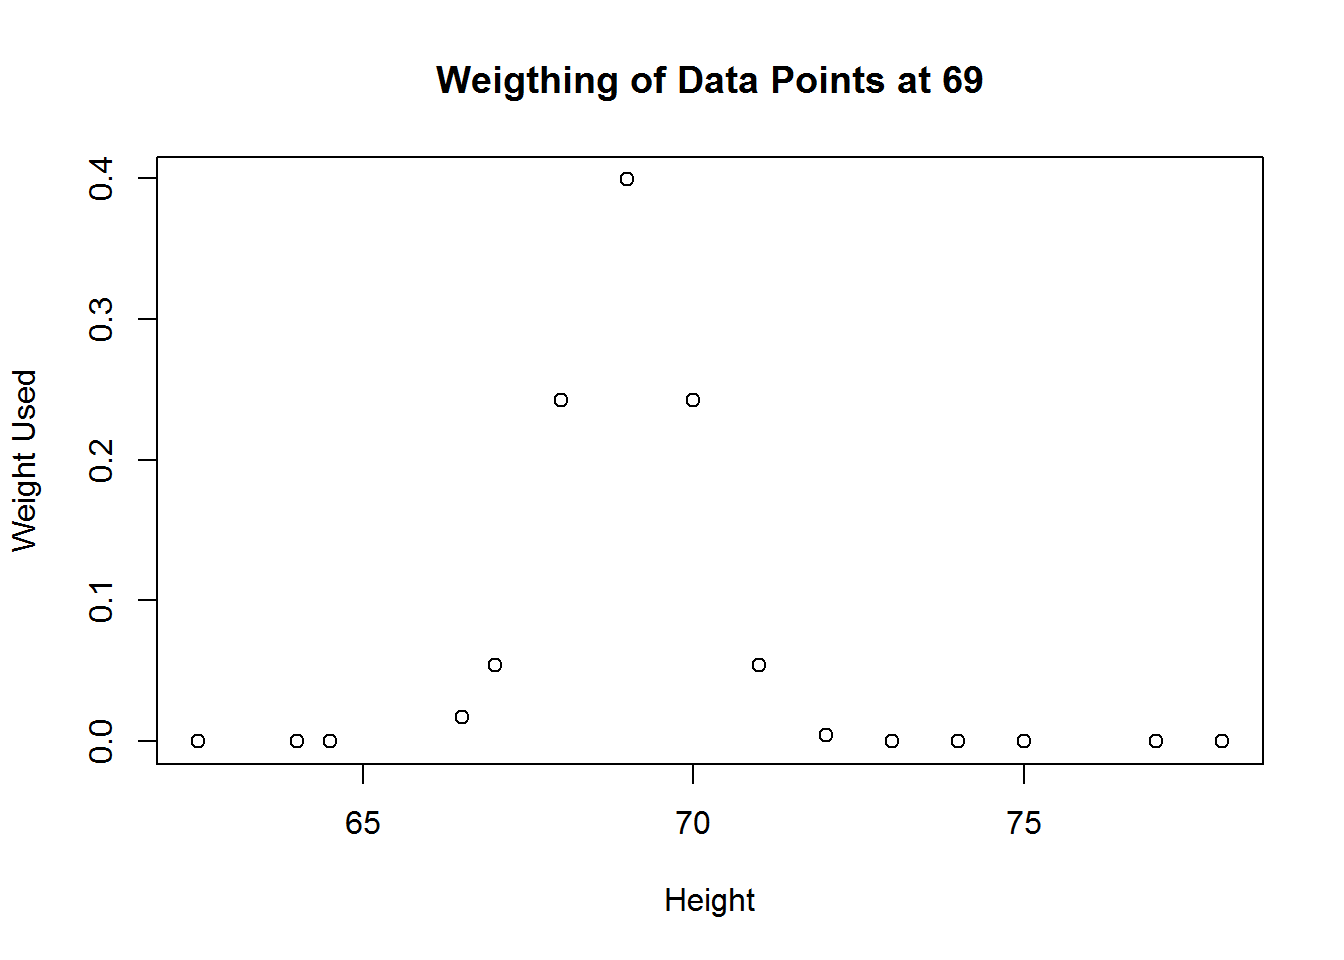
\includegraphics{fastR-Notes_files/figure-latex/unnamed-chunk-195-1.pdf}

Likewise, here it is at the point 73.

\begin{Shaded}
\begin{Highlighting}[]
\KeywordTok{plot}\NormalTok{(Lesson2_Height}\OperatorTok{$}\NormalTok{Height,}\KeywordTok{K4}\NormalTok{(Lesson2_Height}\OperatorTok{$}\NormalTok{Height}\OperatorTok{-}\DecValTok{73}\NormalTok{),}\DataTypeTok{xlab=}\StringTok{"Height"}\NormalTok{,}\DataTypeTok{ylab=}\StringTok{"Weight Used"}\NormalTok{,}\DataTypeTok{main=}\StringTok{"Weigthing of Data Points at 73"}\NormalTok{)}
\end{Highlighting}
\end{Shaded}

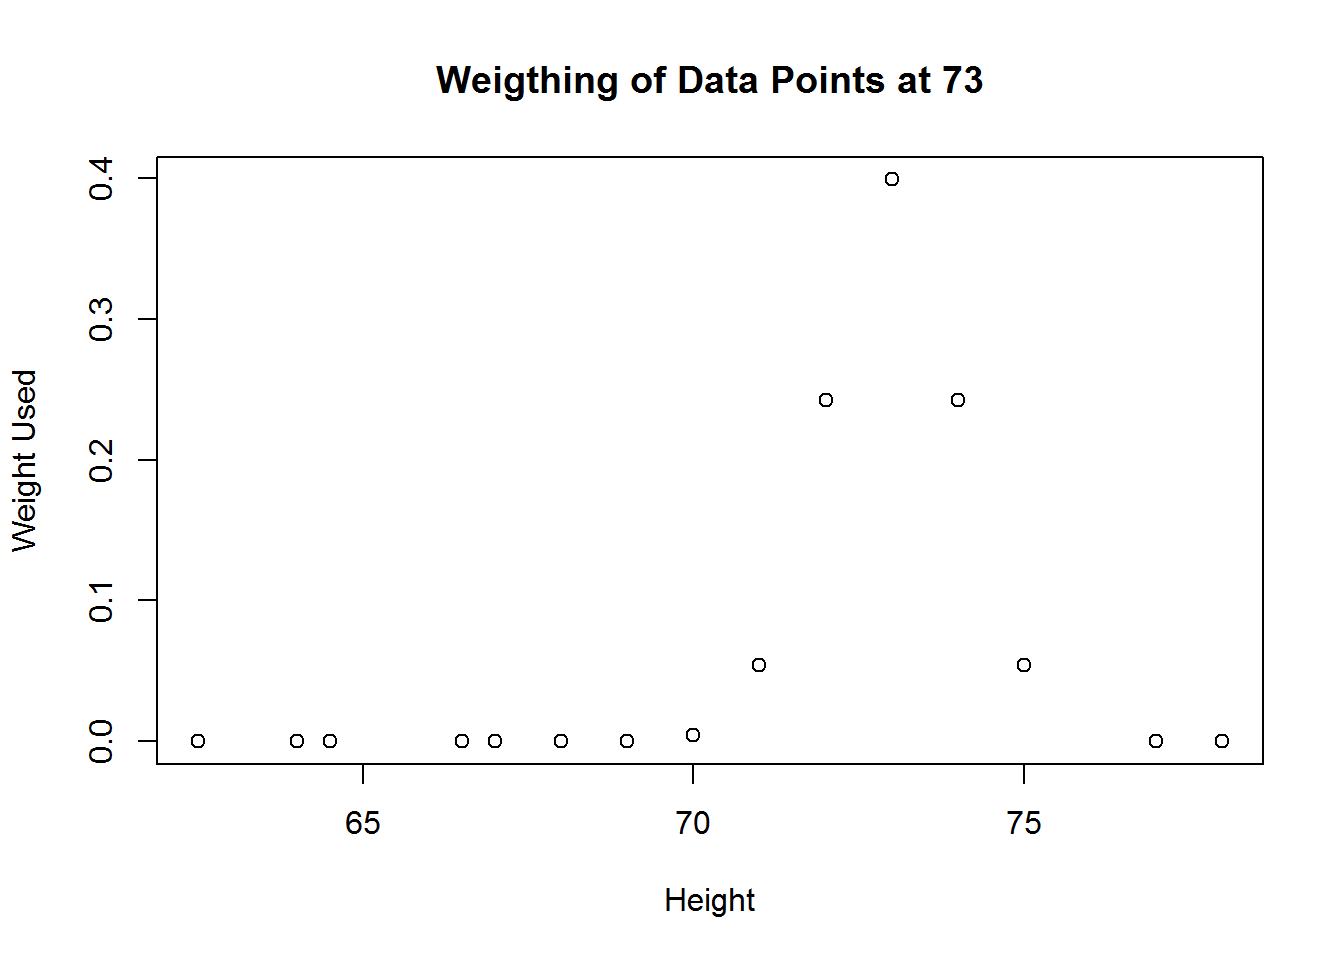
\includegraphics{fastR-Notes_files/figure-latex/unnamed-chunk-196-1.pdf}

Now the kde function, applies the kernel in a moving window across the
data. This gives an estimate of the pdf. For the height data, this is
the estimate.

\begin{Shaded}
\begin{Highlighting}[]
\KeywordTok{plot}\NormalTok{(}\KeywordTok{seq}\NormalTok{(}\DecValTok{64}\NormalTok{,}\DecValTok{75}\NormalTok{,.}\DecValTok{1}\NormalTok{),}\KeywordTok{kde}\NormalTok{(}\DataTypeTok{data=}\NormalTok{Lesson2_Height}\OperatorTok{$}\NormalTok{Height,}\DataTypeTok{kernel =}\NormalTok{ K4)(}\KeywordTok{seq}\NormalTok{(}\DecValTok{64}\NormalTok{,}\DecValTok{75}\NormalTok{,.}\DecValTok{1}\NormalTok{)),}\DataTypeTok{type=}\StringTok{"l"}\NormalTok{,}\DataTypeTok{xlab=}\StringTok{"Height"}\NormalTok{,}\DataTypeTok{ylab=}\StringTok{"Density"}\NormalTok{,}\DataTypeTok{main=}\StringTok{"Density Estimate using Normal Kernel"}\NormalTok{)}
\end{Highlighting}
\end{Shaded}

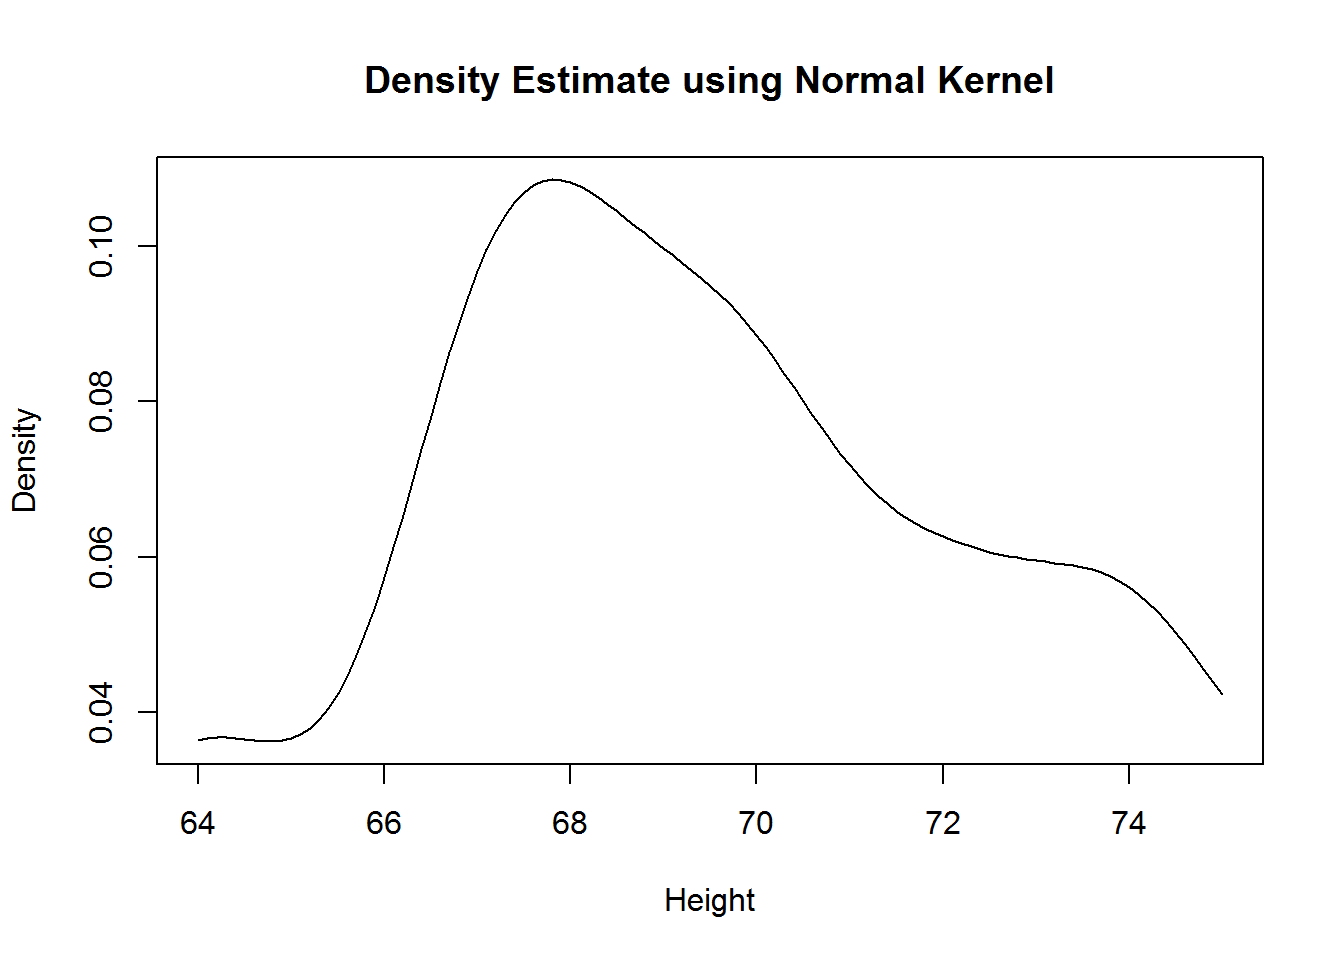
\includegraphics{fastR-Notes_files/figure-latex/unnamed-chunk-197-1.pdf}

Now the width of the kernel will impact the estimate of the pdf. Let's
change K4 to have a different width, standard deviation.

\begin{Shaded}
\begin{Highlighting}[]
\KeywordTok{plot}\NormalTok{(}\KeywordTok{seq}\NormalTok{(}\DecValTok{64}\NormalTok{,}\DecValTok{75}\NormalTok{,.}\DecValTok{1}\NormalTok{),}\KeywordTok{kde}\NormalTok{(}\DataTypeTok{data=}\NormalTok{Lesson2_Height}\OperatorTok{$}\NormalTok{Height,}\DataTypeTok{kernel =}\NormalTok{ K4,}\DataTypeTok{sd=}\NormalTok{.}\DecValTok{5}\NormalTok{)(}\KeywordTok{seq}\NormalTok{(}\DecValTok{64}\NormalTok{,}\DecValTok{75}\NormalTok{,.}\DecValTok{1}\NormalTok{)),}\DataTypeTok{type=}\StringTok{"l"}\NormalTok{,}\DataTypeTok{xlab=}\StringTok{"Height"}\NormalTok{,}\DataTypeTok{ylab=}\StringTok{"Density"}\NormalTok{,}\DataTypeTok{main=}\StringTok{"Density Estimate using Normal Kernel SD=.5"}\NormalTok{)       }
\end{Highlighting}
\end{Shaded}

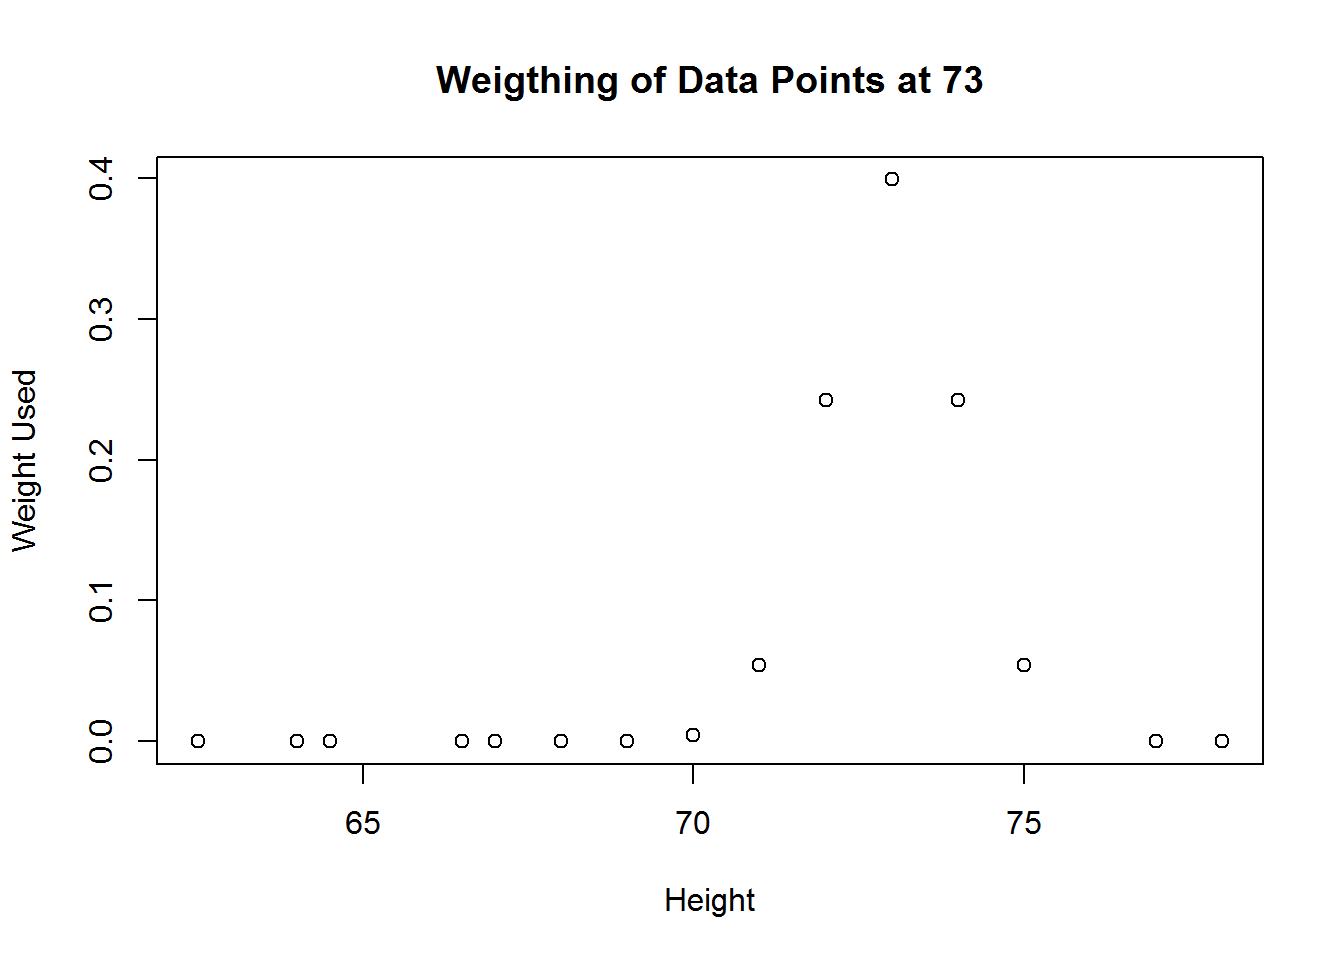
\includegraphics{fastR-Notes_files/figure-latex/unnamed-chunk-198-1.pdf}

This estimate is more sensitive to local data points. In the extreme we
have

\begin{Shaded}
\begin{Highlighting}[]
\KeywordTok{plot}\NormalTok{(}\KeywordTok{seq}\NormalTok{(}\DecValTok{64}\NormalTok{,}\DecValTok{75}\NormalTok{,.}\DecValTok{1}\NormalTok{),}\KeywordTok{kde}\NormalTok{(}\DataTypeTok{data=}\NormalTok{Lesson2_Height}\OperatorTok{$}\NormalTok{Height,}\DataTypeTok{kernel =}\NormalTok{ K4,}\DataTypeTok{sd=}\NormalTok{.}\DecValTok{1}\NormalTok{)(}\KeywordTok{seq}\NormalTok{(}\DecValTok{64}\NormalTok{,}\DecValTok{75}\NormalTok{,.}\DecValTok{1}\NormalTok{)),}\DataTypeTok{type=}\StringTok{"l"}\NormalTok{,}\DataTypeTok{xlab=}\StringTok{"Height"}\NormalTok{,}\DataTypeTok{ylab=}\StringTok{"Density"}\NormalTok{,}\DataTypeTok{main=}\StringTok{"Density Estimate using Normal Kernel SD=.1"}\NormalTok{)}
\end{Highlighting}
\end{Shaded}

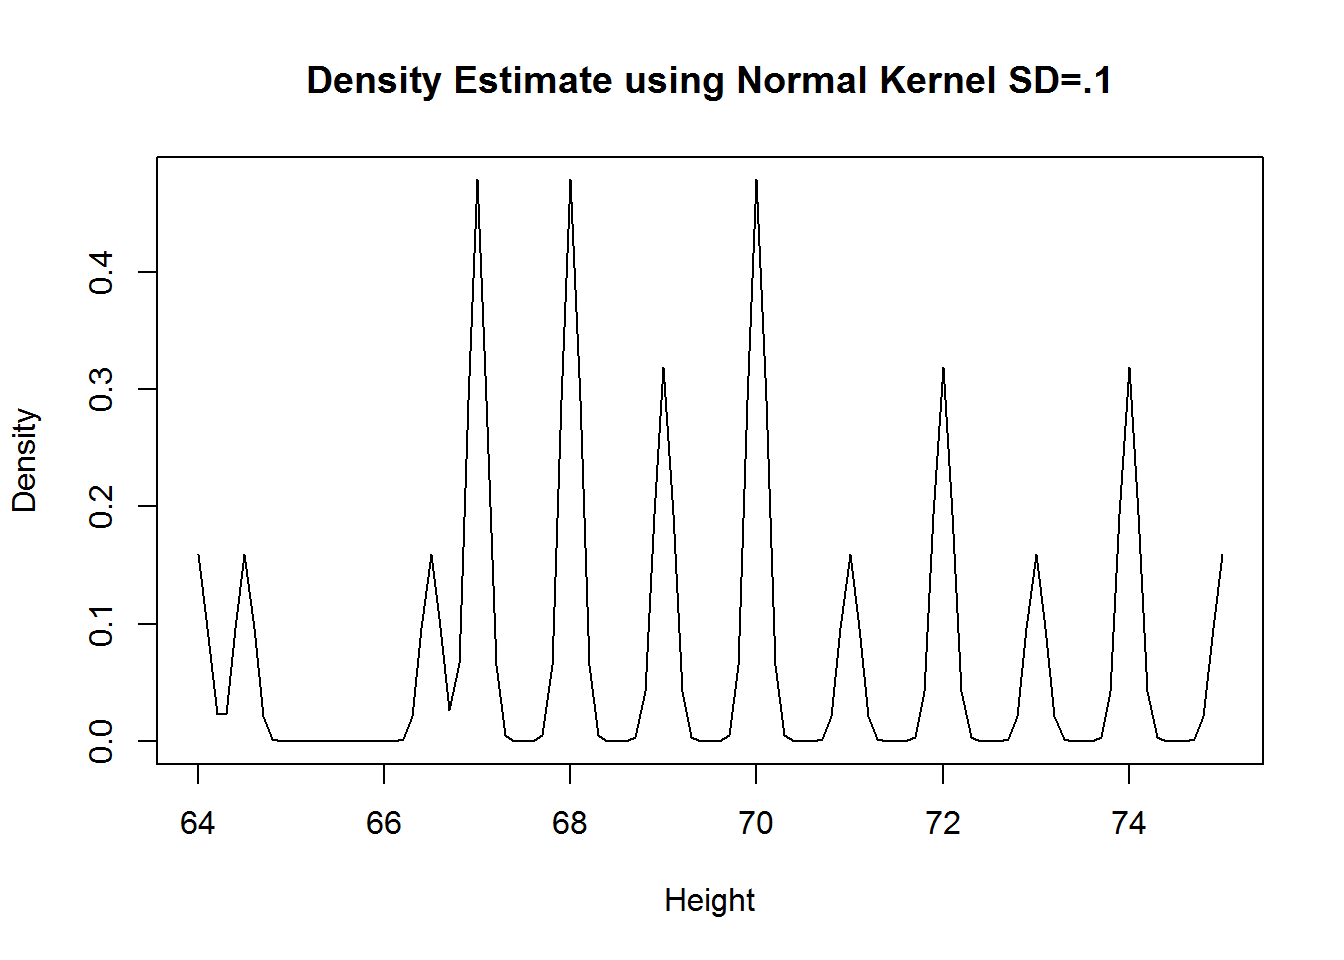
\includegraphics{fastR-Notes_files/figure-latex/unnamed-chunk-199-1.pdf}

The width of the kernel is a tuning parameter that we must choose. This
requires an objective function. The book talks about using mean
integrated square error. Luckily, R has a function that does this for
us.

\begin{Shaded}
\begin{Highlighting}[]
\KeywordTok{densityplot}\NormalTok{(Lesson2_Height}\OperatorTok{$}\NormalTok{Height,}\DataTypeTok{xlab=}\StringTok{"Height"}\NormalTok{,}\DataTypeTok{ylab=}\StringTok{"Density"}\NormalTok{,}\DataTypeTok{main=}\StringTok{"Density Estimate using densityplot"}\NormalTok{)}
\end{Highlighting}
\end{Shaded}

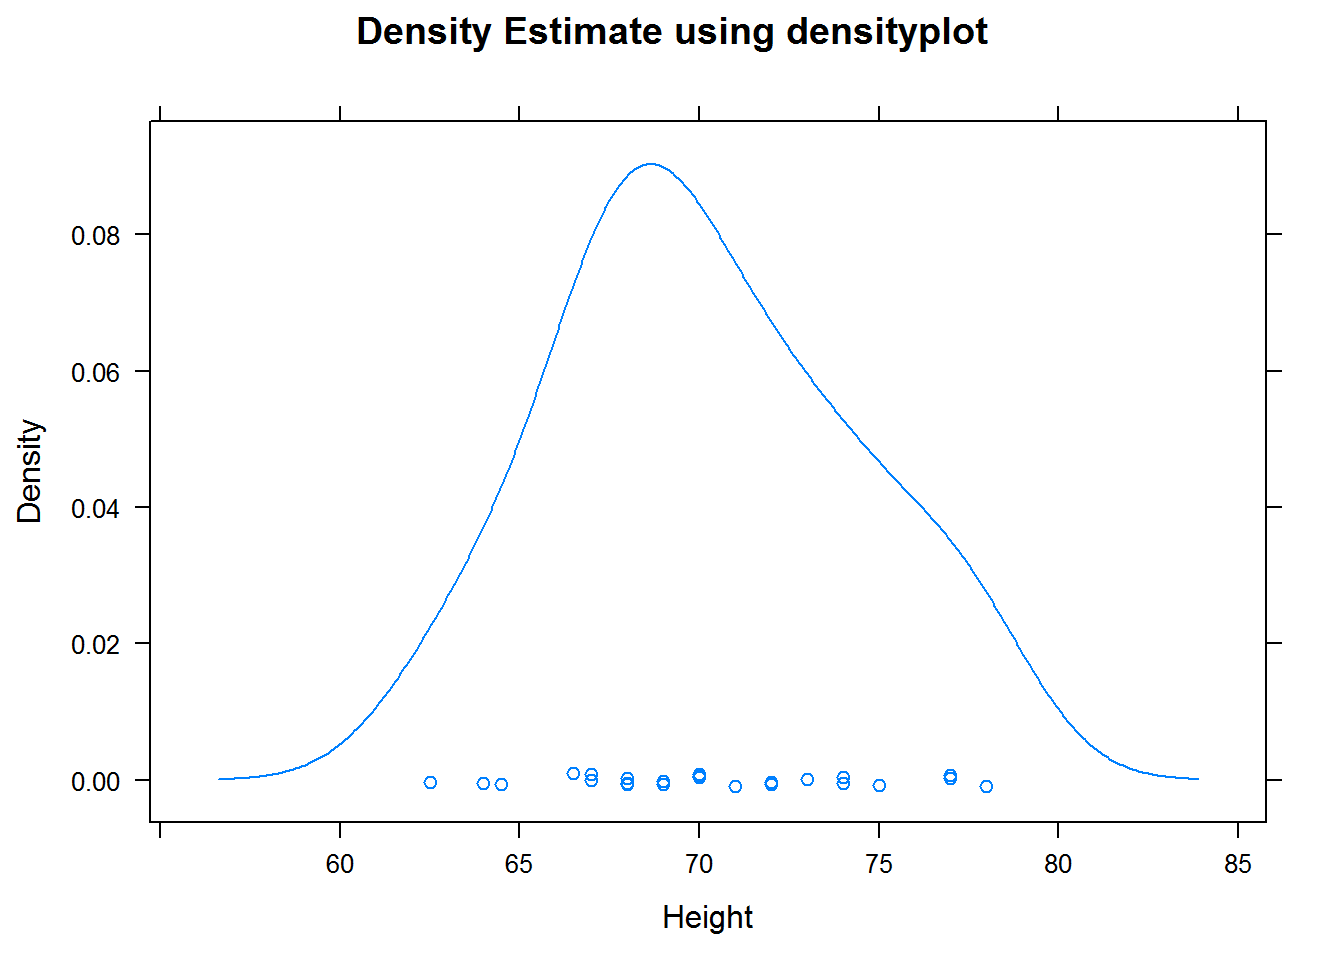
\includegraphics{fastR-Notes_files/figure-latex/unnamed-chunk-200-1.pdf}

We can change the bandwidth directly or just scale the selected
bandwidth using the \texttt{adjust} option.

\begin{Shaded}
\begin{Highlighting}[]
\KeywordTok{densityplot}\NormalTok{(Lesson2_Height}\OperatorTok{$}\NormalTok{Height,}\DataTypeTok{adjust=}\NormalTok{.}\DecValTok{5}\NormalTok{,}\DataTypeTok{xlab=}\StringTok{"Height"}\NormalTok{,}\DataTypeTok{ylab=}\StringTok{"Density"}\NormalTok{,}\DataTypeTok{main=}\StringTok{"Density Estimate using densityplot"}\NormalTok{)}
\end{Highlighting}
\end{Shaded}

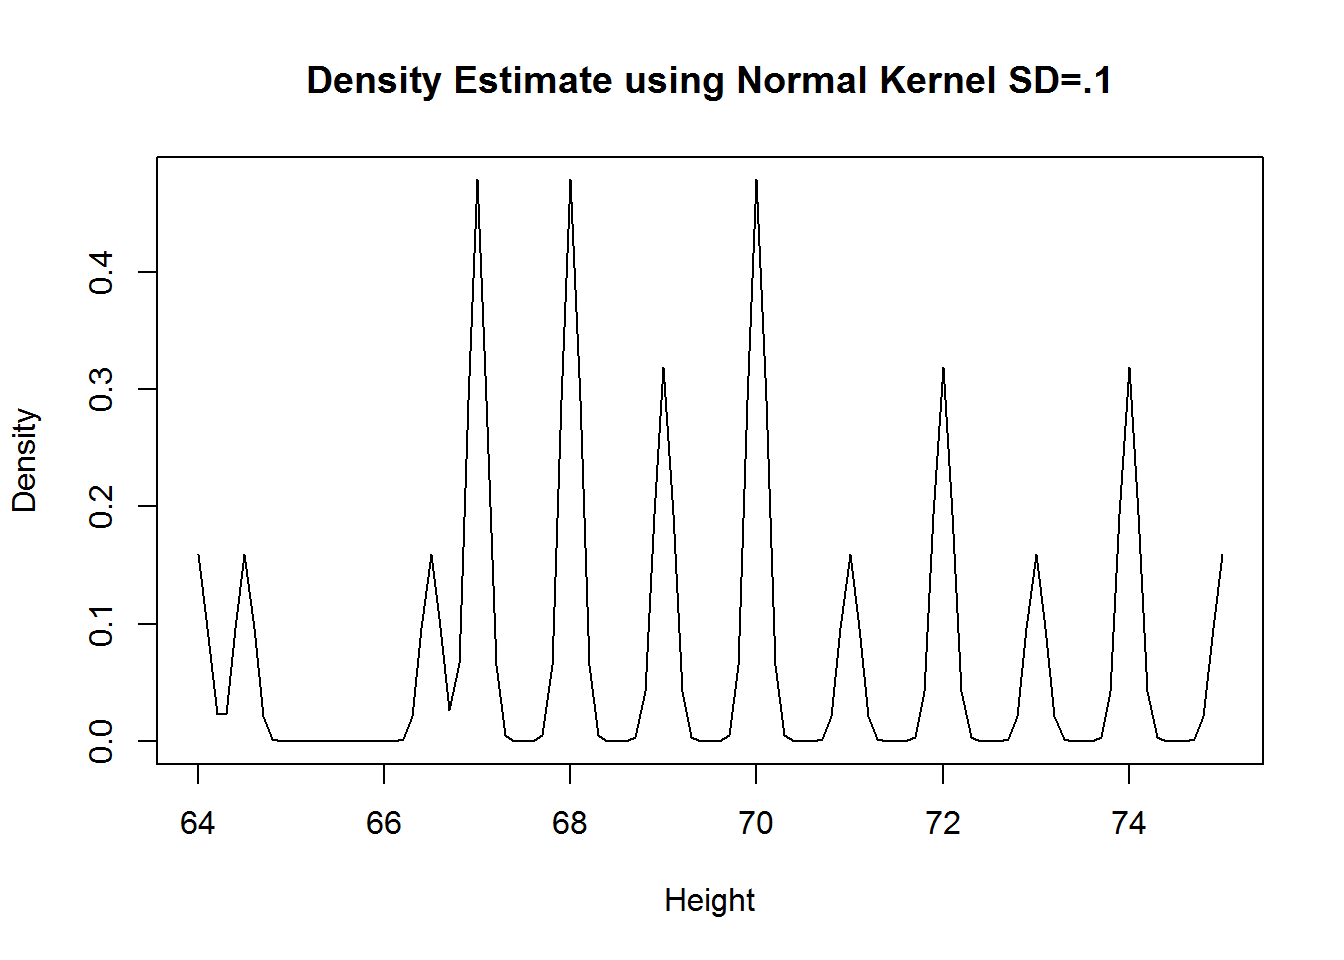
\includegraphics{fastR-Notes_files/figure-latex/unnamed-chunk-201-1.pdf}

\subsection{Practice}\label{practice-4}

Let's work an example using the \texttt{gpa} data in fastR.

\begin{Shaded}
\begin{Highlighting}[]
\KeywordTok{summary}\NormalTok{(gpa)}
\end{Highlighting}
\end{Shaded}

\begin{verbatim}
##       satm          satv            act            gpa       
##  Min.   :370   Min.   :280.0   Min.   :15.0   Min.   :1.704  
##  1st Qu.:560   1st Qu.:560.0   1st Qu.:25.0   1st Qu.:3.034  
##  Median :630   Median :630.0   Median :28.0   Median :3.475  
##  Mean   :623   Mean   :614.6   Mean   :27.7   Mean   :3.352  
##  3rd Qu.:690   3rd Qu.:680.0   3rd Qu.:31.0   3rd Qu.:3.764  
##  Max.   :800   Max.   :800.0   Max.   :35.0   Max.   :4.000
\end{verbatim}

In Chapter 1 we made a histogram to summarize the data. For examples to
summarize the gpa

\begin{Shaded}
\begin{Highlighting}[]
\KeywordTok{histogram}\NormalTok{(gpa}\OperatorTok{$}\NormalTok{gpa)}
\end{Highlighting}
\end{Shaded}

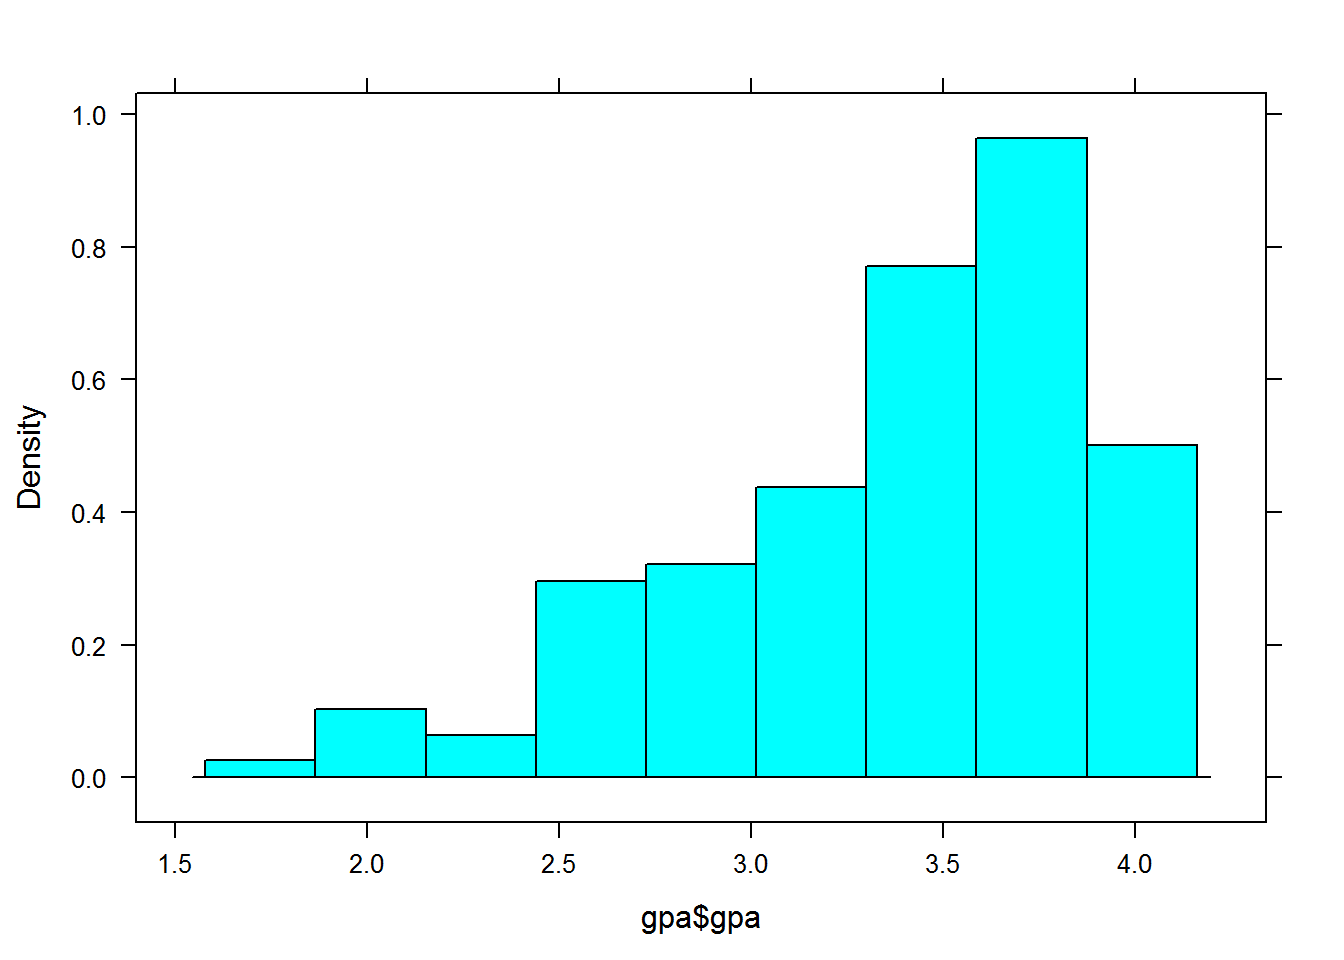
\includegraphics{fastR-Notes_files/figure-latex/unnamed-chunk-203-1.pdf}

Now let's use a density plot:

\begin{Shaded}
\begin{Highlighting}[]
\KeywordTok{densityplot}\NormalTok{(gpa}\OperatorTok{$}\NormalTok{gpa,}\DataTypeTok{xlab=}\StringTok{"GPA"}\NormalTok{)}
\end{Highlighting}
\end{Shaded}

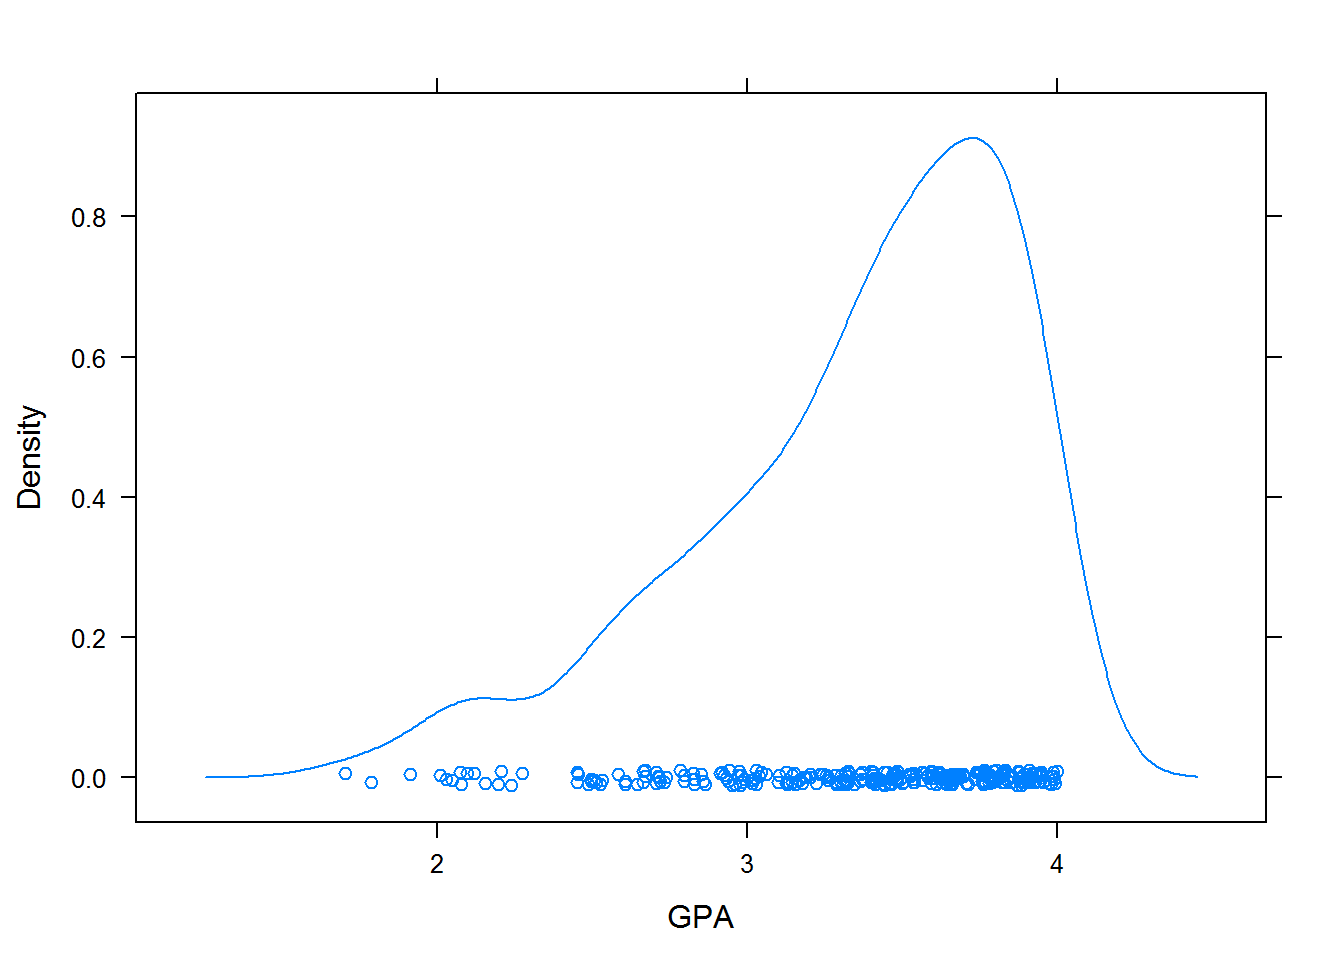
\includegraphics{fastR-Notes_files/figure-latex/unnamed-chunk-204-1.pdf}

I think this gives a better representation of the data. Let's make the
bandwidth 1/2 of the default.

\begin{Shaded}
\begin{Highlighting}[]
\KeywordTok{densityplot}\NormalTok{(gpa}\OperatorTok{$}\NormalTok{gpa,}\DataTypeTok{xlab=}\StringTok{"GPA"}\NormalTok{,}\DataTypeTok{adjust=}\NormalTok{.}\DecValTok{5}\NormalTok{)}
\end{Highlighting}
\end{Shaded}

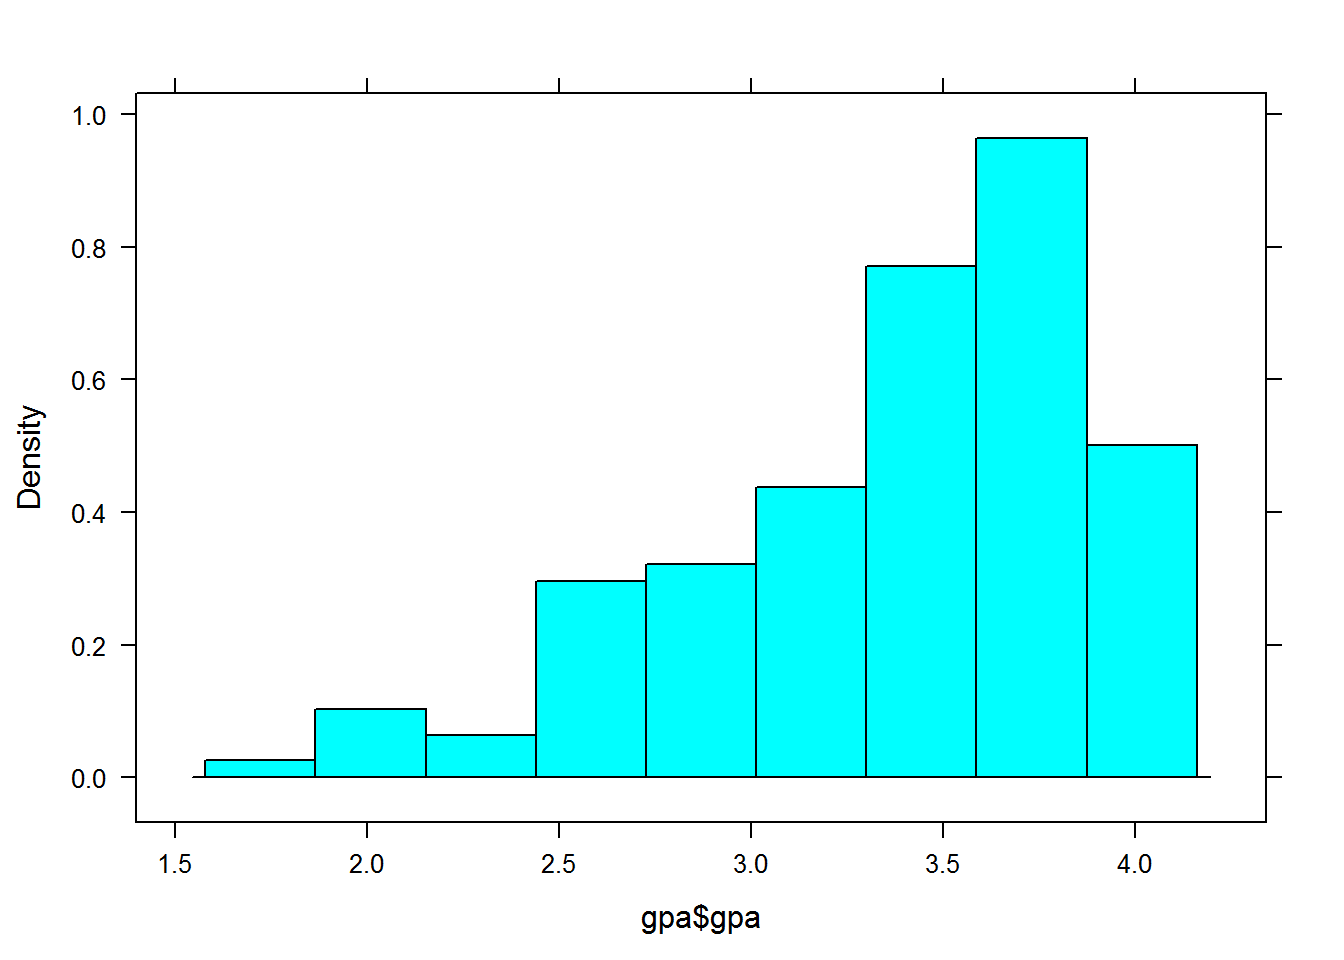
\includegraphics{fastR-Notes_files/figure-latex/unnamed-chunk-205-1.pdf}

This is picking up more of the noise. Let's make the bandwidth larger
which may cause too much smoothing.

\begin{Shaded}
\begin{Highlighting}[]
\KeywordTok{densityplot}\NormalTok{(gpa}\OperatorTok{$}\NormalTok{gpa,}\DataTypeTok{xlab=}\StringTok{"GPA"}\NormalTok{,}\DataTypeTok{adjust=}\DecValTok{4}\NormalTok{)}
\end{Highlighting}
\end{Shaded}

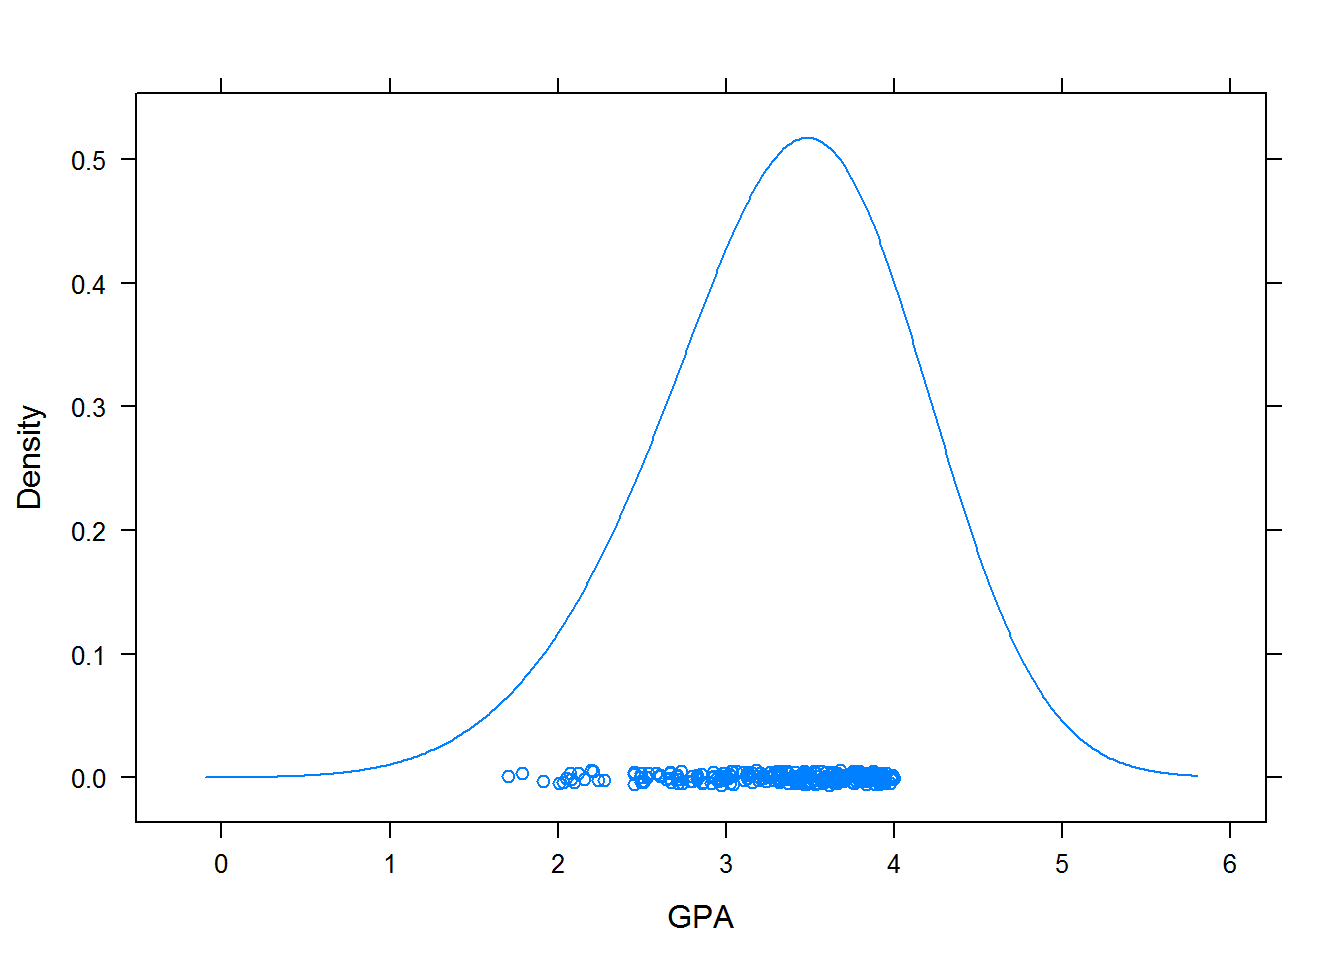
\includegraphics{fastR-Notes_files/figure-latex/unnamed-chunk-206-1.pdf}

\subsection{Q-Q Plots}\label{q-q-plots}

Next, we would like to be able to justify a certain distribution as a
reasonable model for our data. For example, with the gpa data, you may
be asked if it is valid to assume that the data is normally distributed.
One way to answer this is by comparing the empirical quantiles from the
data with the quantiles from the reference distribution. If it is a good
match, the scatterplot will have the data points lying on a straight
line. The function \texttt{xqqmath} in the fastR package makes this easy
for us.

Let's start with the height data

\begin{Shaded}
\begin{Highlighting}[]
\KeywordTok{xqqmath}\NormalTok{(}\OperatorTok{~}\NormalTok{Height,}\DataTypeTok{data=}\NormalTok{Lesson2_Height)}
\end{Highlighting}
\end{Shaded}

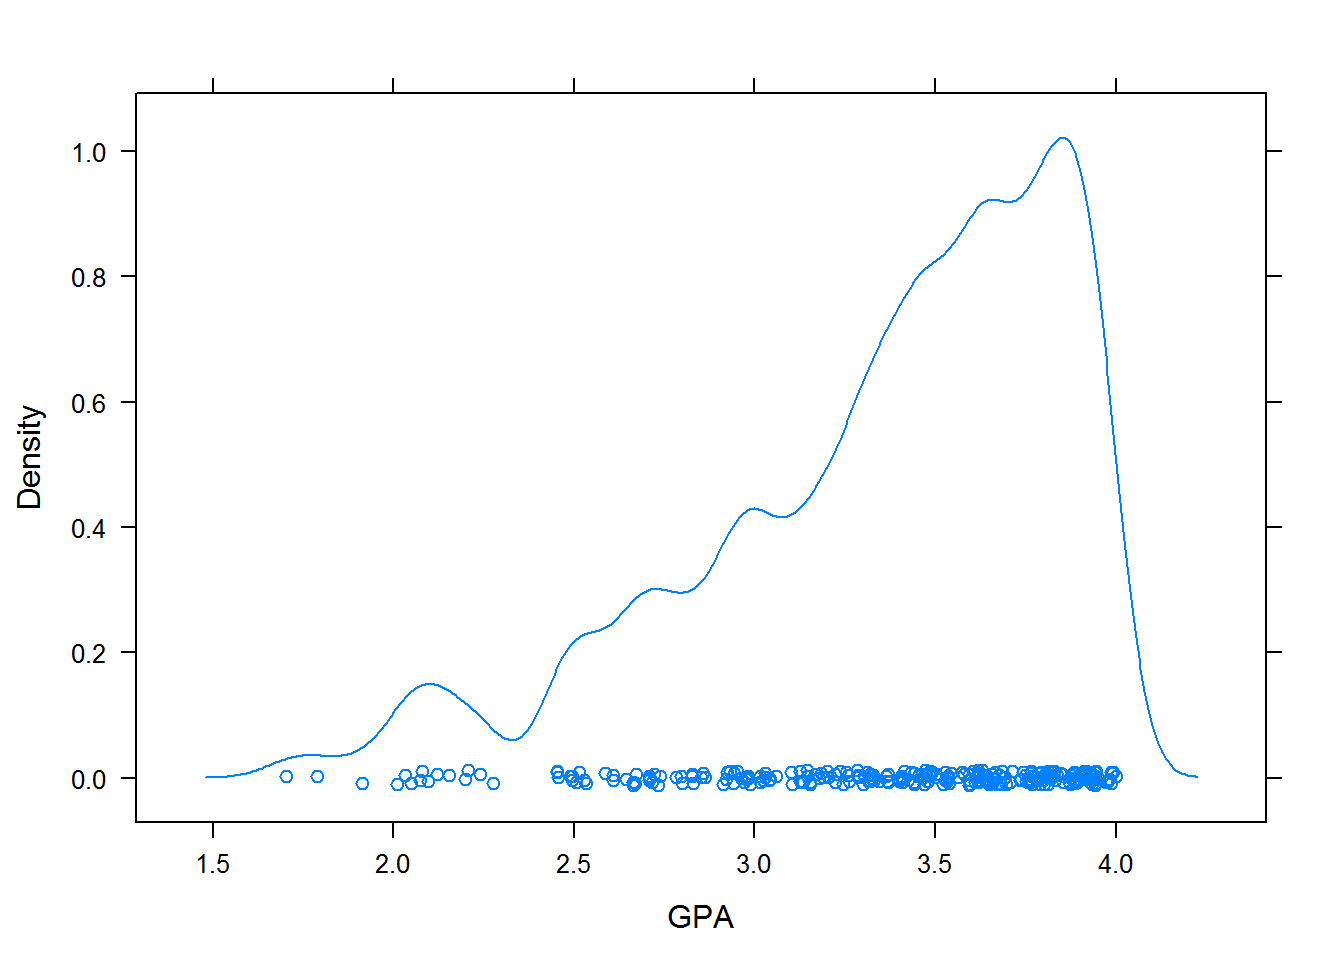
\includegraphics{fastR-Notes_files/figure-latex/unnamed-chunk-207-1.pdf}

\begin{Shaded}
\begin{Highlighting}[]
\KeywordTok{xqqmath}\NormalTok{(}\OperatorTok{~}\NormalTok{Height,}\DataTypeTok{data=}\NormalTok{Lesson2_Height,}\DataTypeTok{fitline=}\OtherTok{TRUE}\NormalTok{)}
\end{Highlighting}
\end{Shaded}

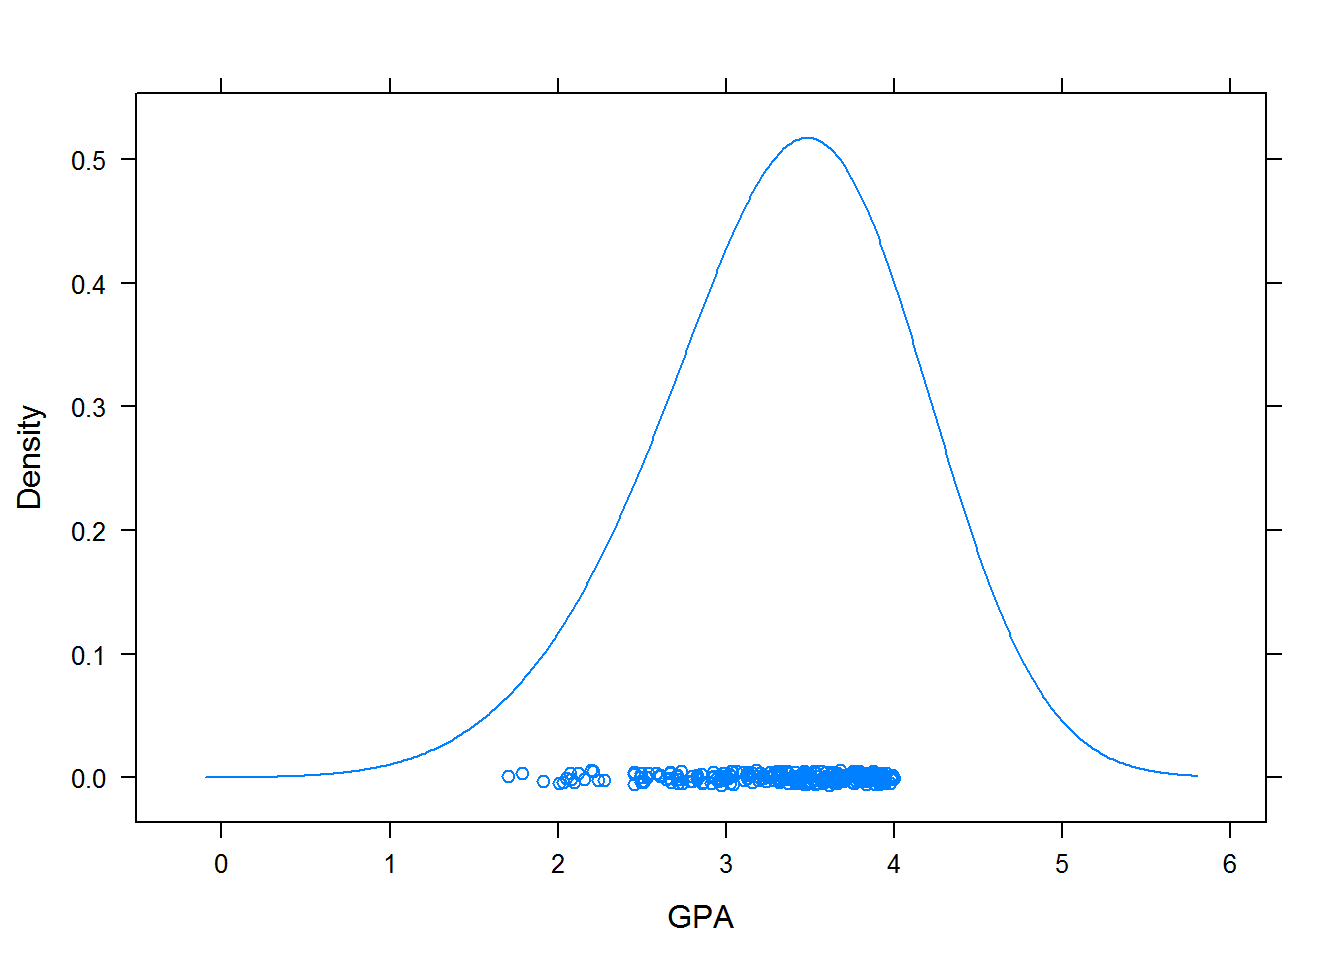
\includegraphics{fastR-Notes_files/figure-latex/unnamed-chunk-208-1.pdf}

This plot is subjective. It is finding the empirical quantiles and then
plotting these against the same quantiles from selected distribution,
the normal by default. If the data comes from the selected distribution,
the quantiles lie along a straight line. The data points will not be
perfectly along the line, but as long as they are close, we feel
comfortable with our assumption. As a follow-up, we can also check how
sensitive our analysis is to the distributional assumption.

We can build our own q-q plot just to understand the process.

We have 25 data points that we will sort. The empirical quantiles are
found by noticing that each data point is 1/25 or .04 of the data. We
don't want to start or stop at 0 or 1, so let's split the .04 and start
at .02 and end at .98. Thus the quantiles are

\begin{Shaded}
\begin{Highlighting}[]
 \KeywordTok{seq}\NormalTok{(.}\DecValTok{02}\NormalTok{,.}\DecValTok{98}\NormalTok{,.}\DecValTok{04}\NormalTok{)}
\end{Highlighting}
\end{Shaded}

\begin{verbatim}
##  [1] 0.02 0.06 0.10 0.14 0.18 0.22 0.26 0.30 0.34 0.38 0.42 0.46 0.50 0.54
## [15] 0.58 0.62 0.66 0.70 0.74 0.78 0.82 0.86 0.90 0.94 0.98
\end{verbatim}

Now, we must decide what to do with ties. We could just treat them as
separate data points or we can accumulate all the probability at each
point.

Here is the first method

\begin{Shaded}
\begin{Highlighting}[]
\KeywordTok{plot}\NormalTok{(}\KeywordTok{qnorm}\NormalTok{(}\KeywordTok{seq}\NormalTok{(.}\DecValTok{02}\NormalTok{,.}\DecValTok{98}\NormalTok{,.}\DecValTok{04}\NormalTok{)),}\KeywordTok{sort}\NormalTok{(Lesson2_Height}\OperatorTok{$}\NormalTok{Height),}\DataTypeTok{xlab=}\StringTok{"qnorm"}\NormalTok{,}\DataTypeTok{ylab=}\StringTok{"Height"}\NormalTok{,}\DataTypeTok{main=}\StringTok{"My Own Q-Q Plot"}\NormalTok{)}
\end{Highlighting}
\end{Shaded}

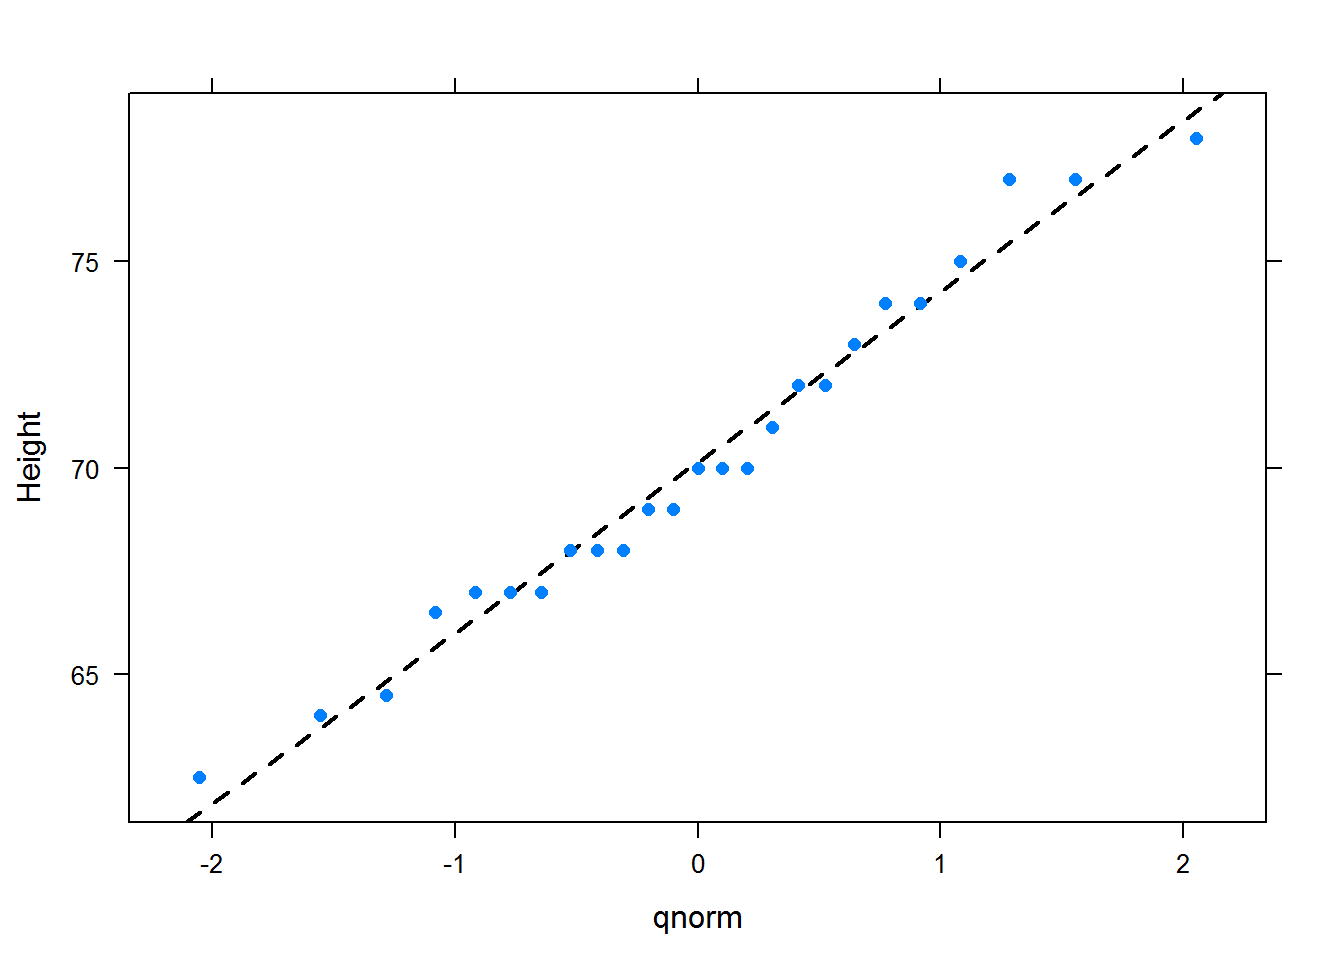
\includegraphics{fastR-Notes_files/figure-latex/unnamed-chunk-210-1.pdf}

The second method is harder to do. I must table the numbers

\begin{Shaded}
\begin{Highlighting}[]
\KeywordTok{table}\NormalTok{(Lesson2_Height}\OperatorTok{$}\NormalTok{Height)}
\end{Highlighting}
\end{Shaded}

\begin{verbatim}
## 
## 62.5   64 64.5 66.5   67   68   69   70   71   72   73   74   75   77   78 
##    1    1    1    1    3    3    2    3    1    2    1    2    1    2    1
\end{verbatim}

So at 67, the quantile will jump by 0.12 instead of 0.04. Thus the
empirical quantiles are

\begin{Shaded}
\begin{Highlighting}[]
\NormalTok{temp<-}\KeywordTok{c}\NormalTok{(}\FloatTok{0.02}\NormalTok{,}\FloatTok{0.06}\NormalTok{,}\FloatTok{0.10}\NormalTok{,}\FloatTok{0.14}\NormalTok{,}\FloatTok{0.26}\NormalTok{,}\FloatTok{0.38}\NormalTok{,}\FloatTok{0.46}\NormalTok{,}\FloatTok{0.58}\NormalTok{,}\FloatTok{0.62}\NormalTok{,}\FloatTok{0.70}\NormalTok{,}\FloatTok{0.74}\NormalTok{,}\FloatTok{0.82}\NormalTok{,}\FloatTok{0.86}\NormalTok{,}\FloatTok{0.94}\NormalTok{,}\FloatTok{0.98}\NormalTok{)}
\end{Highlighting}
\end{Shaded}

\begin{Shaded}
\begin{Highlighting}[]
\KeywordTok{plot}\NormalTok{(}\KeywordTok{qnorm}\NormalTok{(temp),}\KeywordTok{sort}\NormalTok{(}\KeywordTok{unique}\NormalTok{(Lesson2_Height}\OperatorTok{$}\NormalTok{Height)),}\DataTypeTok{xlab=}\StringTok{"qnorm"}\NormalTok{,}\DataTypeTok{ylab=}\StringTok{"Height"}\NormalTok{,}\DataTypeTok{main=}\StringTok{"My Own Q-Q Plot"}\NormalTok{)}
\end{Highlighting}
\end{Shaded}

\includegraphics{fastR-Notes_files/figure-latex/unnamed-chunk-213-1.pdf}

Back to \texttt{xqqmath}, the default method of inserting a line is to
put it through the first and third quartiles. Another is the fit a line
by estimating the mean and standard deviation. We will learn about these
ideas later.

\begin{Shaded}
\begin{Highlighting}[]
\KeywordTok{xqqmath}\NormalTok{(}\OperatorTok{~}\NormalTok{Height,}\DataTypeTok{data=}\NormalTok{Lesson2_Height,}\DataTypeTok{fitline=}\OtherTok{TRUE}\NormalTok{)}
\end{Highlighting}
\end{Shaded}

\includegraphics{fastR-Notes_files/figure-latex/unnamed-chunk-214-1.pdf}

From our data, the normal assumption is not bad.

Let's try it for the \texttt{gpa} data.

\begin{Shaded}
\begin{Highlighting}[]
\KeywordTok{xqqmath}\NormalTok{(}\OperatorTok{~}\NormalTok{gpa,}\DataTypeTok{data=}\NormalTok{gpa)}
\end{Highlighting}
\end{Shaded}

\includegraphics{fastR-Notes_files/figure-latex/unnamed-chunk-215-1.pdf}

From this plot we can see that our data is skewed to the left compared
with the normal distribution. Look at the right side of the figure, if
the quantiles from the data increased as fast as those from the normal
the points would fall along the line. Using a normal distribution for
this data is not a good idea.

Maybe if we put gpa on a scale of 0 to 1 and then compare with a Beta,
that is a better fit.

\begin{Shaded}
\begin{Highlighting}[]
\NormalTok{mygpa<-gpa}\OperatorTok{$}\NormalTok{gpa}\OperatorTok{/}\DecValTok{4}
\KeywordTok{densityplot}\NormalTok{(mygpa)}
\end{Highlighting}
\end{Shaded}

\includegraphics{fastR-Notes_files/figure-latex/unnamed-chunk-216-1.pdf}

Next chapter we will look at estimating the parameters of a
distributions; for now we will a Beta(5,2)

\begin{Shaded}
\begin{Highlighting}[]
\KeywordTok{plot}\NormalTok{(}\KeywordTok{seq}\NormalTok{(}\DecValTok{0}\NormalTok{,}\DecValTok{1}\NormalTok{,.}\DecValTok{01}\NormalTok{),}\KeywordTok{dbeta}\NormalTok{(}\KeywordTok{seq}\NormalTok{(}\DecValTok{0}\NormalTok{,}\DecValTok{1}\NormalTok{,.}\DecValTok{01}\NormalTok{),}\DecValTok{5}\NormalTok{,}\DecValTok{2}\NormalTok{),}\DataTypeTok{type=}\StringTok{"l"}\NormalTok{)}
\end{Highlighting}
\end{Shaded}

\includegraphics{fastR-Notes_files/figure-latex/unnamed-chunk-217-1.pdf}

\begin{Shaded}
\begin{Highlighting}[]
\NormalTok{qb<-}\ControlFlowTok{function}\NormalTok{(x)\{}\KeywordTok{qbeta}\NormalTok{(x,}\DecValTok{5}\NormalTok{,}\DecValTok{2}\NormalTok{)\}}
\KeywordTok{xqqmath}\NormalTok{(}\OperatorTok{~}\NormalTok{mygpa,}\DataTypeTok{distribution=}\NormalTok{qb)}
\end{Highlighting}
\end{Shaded}

\includegraphics{fastR-Notes_files/figure-latex/unnamed-chunk-218-1.pdf}

There are still some problems with the fit but it is better. The Beta
has a longer tail to the right versus our data.

Finding the parameters using ideas from Chapter 4

\begin{Shaded}
\begin{Highlighting}[]
\KeywordTok{plot}\NormalTok{(}\KeywordTok{seq}\NormalTok{(}\DecValTok{0}\NormalTok{,}\DecValTok{1}\NormalTok{,.}\DecValTok{01}\NormalTok{),}\KeywordTok{dbeta}\NormalTok{(}\KeywordTok{seq}\NormalTok{(}\DecValTok{0}\NormalTok{,}\DecValTok{1}\NormalTok{,.}\DecValTok{01}\NormalTok{),}\FloatTok{6.156995}\NormalTok{,}\FloatTok{1.189227}\NormalTok{),}\DataTypeTok{type=}\StringTok{"l"}\NormalTok{)}
\end{Highlighting}
\end{Shaded}

\includegraphics{fastR-Notes_files/figure-latex/unnamed-chunk-219-1.pdf}

\begin{Shaded}
\begin{Highlighting}[]
\NormalTok{qb<-}\ControlFlowTok{function}\NormalTok{(x)\{}\KeywordTok{qbeta}\NormalTok{(x,}\FloatTok{6.156995}\NormalTok{,}\FloatTok{1.189227}\NormalTok{)\}}
\KeywordTok{xqqmath}\NormalTok{(}\OperatorTok{~}\NormalTok{mygpa,}\DataTypeTok{distribution=}\NormalTok{qb)}
\end{Highlighting}
\end{Shaded}

\includegraphics{fastR-Notes_files/figure-latex/unnamed-chunk-220-1.pdf}

Do Homework 3.38

\hypertarget{L17}{\section{Continuous Joint Distributions}\label{L17}}

\subsection{Objectives}\label{objectives-16}

\begin{enumerate}
\def\labelenumi{\arabic{enumi}.}
\tightlist
\item
  From a joint pdf find the marginal and conditional pdf\\
\item
  Calculate marginal, joint, and conditional probabilities using
  integration\\
\item
  Determine if two random variables are independent\\
\item
  Find the distribution of a sum of independent random variables, the
  most important case being normal random variables
\end{enumerate}

\subsection{Background}\label{background-2}

With continuous random variables, we use all the same ideas from joint
distributions for discrete as well as the ideas from univariate
continuous except

\begin{enumerate}
\def\labelenumi{\arabic{enumi}.}
\tightlist
\item
  To find \(P(X<x|Y=y)\) we need to find the conditional pdf
  \({f_{X,Y}(x,y) \over f_{Y}(y)}|_{Y=y}\)\\
\item
  Independence, iff \(f_{X,Y}(x,y)=g(x)h(y)\) and the domain is
  rectangular \(a \leq x \leq b\) and \(c \leq y \leq d\) for real
  numbers \(a,b,c,\) and \(d\).\\
\item
  Distribution of a sum of independent random variables, you can use the
  moment generating function and Thm 3.7.10.
\end{enumerate}

Note: most of the problems in this section require Calc III ideas. Draw
a picture of the domain to setup limits of integration. Also, for
inequalities, set as an equality and then pick a point on one side of
the line to check if it meets the condition of the inequality.

\subsection{Practice}\label{practice-5}

To make use of the ideas we will practice

\begin{enumerate}
\def\labelenumi{\arabic{enumi}.}
\tightlist
\item
  Problem 3.45\\
\end{enumerate}

\begin{enumerate}
\def\labelenumi{\alph{enumi}.}
\tightlist
\item
  Find joint pdf and verify it is a proper pdf\\
\item
  Find the probability that Alice and Bob arrive before 5:15\\
\item
  Find the probability that Alice arrives before Bob\\
\item
  Find the probability that Alice arrives before 5:30 given that Bob
  arrives before 5:30\\
\item
  Find the probability that Alice arrives before 5:30 given that Bob
  arrives at exactly 5:30
\end{enumerate}

\begin{enumerate}
\def\labelenumi{\arabic{enumi}.}
\setcounter{enumi}{1}
\tightlist
\item
  Change the problem to state that Alice will always arrive before Bob.
  Thus the domain is \(5 \leq x < y \leq 6\). Assume the joint pdf is
  uniform.
\end{enumerate}

\begin{enumerate}
\def\labelenumi{\alph{enumi}.}
\tightlist
\item
  Find joint pdf and verify it is a proper pdf\\
\item
  Find the probability that Alice and Bob arrive before 5:15\\
\item
  Find the probability that Alice arrives before Bob\\
\item
  Find the probability that Alice arrives before 5:30 given that Bob
  arrives before 5:45\\
\item
  Find the probability that Alice arrives before 5:30 given that Bob
  arrives at 5:45\\
\item
  Are X and Y independent?
\end{enumerate}

\begin{enumerate}
\def\labelenumi{\arabic{enumi}.}
\setcounter{enumi}{2}
\item
  Problem 3.51
\item
  If \(X_{i} \overset{iid}{\sim} \mbox{Norm} (2,3)\) what is the
  distribution of \(\bar{X}\) for a sample size of 10?
\end{enumerate}

Here is some interesting code to perform multivariate integration.

\begin{Shaded}
\begin{Highlighting}[]
\NormalTok{f<-}\ControlFlowTok{function}\NormalTok{(x,y)}\DecValTok{1}\OperatorTok{/}\DecValTok{4}\OperatorTok{*}\NormalTok{(x}\OperatorTok{+}\DecValTok{2}\OperatorTok{*}\NormalTok{y)}
\KeywordTok{integrate}\NormalTok{(}\ControlFlowTok{function}\NormalTok{(y)\{}\KeywordTok{sapply}\NormalTok{(y,}\ControlFlowTok{function}\NormalTok{(y)\{}\KeywordTok{integrate}\NormalTok{(}\ControlFlowTok{function}\NormalTok{(x)}\KeywordTok{f}\NormalTok{(x,y),y,}\DecValTok{2}\NormalTok{)}\OperatorTok{$}\NormalTok{value\})\},}\DecValTok{0}\NormalTok{,}\DecValTok{1}\NormalTok{)}
\end{Highlighting}
\end{Shaded}

\begin{verbatim}
## 0.7916667 with absolute error < 8.8e-15
\end{verbatim}

\begin{Shaded}
\begin{Highlighting}[]
\KeywordTok{integrate}\NormalTok{(}\ControlFlowTok{function}\NormalTok{(y)\{}\KeywordTok{sapply}\NormalTok{(y,}\ControlFlowTok{function}\NormalTok{(y)\{}\KeywordTok{integrate}\NormalTok{(}\ControlFlowTok{function}\NormalTok{(x)}\KeywordTok{f}\NormalTok{(x,y),}\DecValTok{0}\NormalTok{,}\DecValTok{2}\NormalTok{)}\OperatorTok{$}\NormalTok{value\})\},}\DecValTok{0}\NormalTok{,}\DecValTok{1}\NormalTok{)}
\end{Highlighting}
\end{Shaded}

\begin{verbatim}
## 1 with absolute error < 1.1e-14
\end{verbatim}

\chapter{Parameter Estimation and Testing}\label{Chpt4}

The fourth chapter is completed in seven lessons. Sections 4.1 and 4.2
are combined into one lesson. The same is true for sections 4.6 and 4.7
as well as 4.8 and 4.9. Section 4.6 tends to be technical and
mathematical so we only require the students to know Lemma 4.6.1,
Theorem 4.6.5, Definition 4.6.6, Lemma 4.6.7, Lemma 4.6.8, and Corollary
4.6.9.

\hypertarget{L18}{\section{Method of Moments}\label{L18}}

\subsection{Objectives}\label{objectives-17}

\begin{enumerate}
\def\labelenumi{\arabic{enumi}.}
\tightlist
\item
  Know and properly use the new terminology and notation to include but
  not limited to, sample moment, around origin and sample mean,
  parameter, and independent and identically distributed\\
\item
  Find parameter estimates, univariate and multivariate, using the
  method of moments, this may include using a root solver\\
\item
  Know the relationship between the second sample moment about the
  sample mean and the sample variance
\end{enumerate}

\subsection{Introduction}\label{introduction}

The book does a great job introducing the idea of statistical
mathematical models. Typically in this class, we want to use them by
using a sample and model of the population to make an inference about
the population. In Math 378, we will start to use them to make
predictions. We also see this a little at the end of this course when we
introduce linear regression.

There are several issues that we have to handle. First we have to decide
which model is appropriate. We already partially addressed this with the
Q-Q plots of last chapter. The second issue is how to estimate
parameters for the model. That is this lesson. Finally, we will have to
address how to make inferences about the population parameter from the
sample estimate.

\subsection{Method of Moment
Estimates}\label{method-of-moment-estimates}

Once we have decided on a model for the population, we typically want to
estimate parameters by using data from a sample. The idea that we will
use is simply that we will equate sample moments to population moments
and then try to solve for the parameter(s) of interest.

The book defines sample moments both around the origin and around the
sample mean. See page 180. Do not confuse these with the population
moments from Chapter 3, see page 126. Those are moments for the entire
population and not just a sample.

As a comparison, here are the formulas for the \texttt{kth} sample
moment about the origin and the \texttt{kth} moment about the origin.

\[\hat{\mu}_{k}={1 \over n}\sum_{i=1}^n\left( x_{i} \right)^k\]
\[\mu_{k}=E\left(x^k \right)\]

Notice the \texttt{hat} on the sample moment. This notation is used to
denote an estimate.

\subsection{Example}\label{example-1}

Suppose I have some data

\begin{Shaded}
\begin{Highlighting}[]
\NormalTok{Les22Data}
\end{Highlighting}
\end{Shaded}

\begin{verbatim}
##  [1] 3.1014985 1.7371363 5.2919977 1.4964655 2.6323325 2.8416648 2.1685008
##  [8] 4.2943013 1.2207340 4.3090411 2.1333155 3.2770935 0.7652807 2.1089708
## [15] 2.5630758 3.3944054 3.2639452 3.9491399 1.4743717 1.0406365 2.2933009
## [22] 5.9144906 4.4901816 1.8617249 1.3017419 1.1851448 3.0619336 3.9773334
## [29] 1.5961078 2.3282182 2.9802030 2.4739417 3.2587091 2.4006987 2.0145723
## [36] 3.9677253 3.1962093 3.4056244 2.6510675 2.4499892
\end{verbatim}

Let's plot it:

\begin{Shaded}
\begin{Highlighting}[]
\KeywordTok{library}\NormalTok{(fastR)}
\end{Highlighting}
\end{Shaded}

\begin{Shaded}
\begin{Highlighting}[]
\KeywordTok{densityplot}\NormalTok{(Les22Data)}
\end{Highlighting}
\end{Shaded}

\includegraphics{fastR-Notes_files/figure-latex/unnamed-chunk-225-1.pdf}

I don't know the population mean, what would be a reasonable estimate?
The sample mean is an obvious choice. Thus my estimate of \(E(X)\) which
is also called \(\mu\) is \(\hat{\mu}\).

Again, the key idea from this section is that the population moments are
a function of the parameters of the distribution. Thus we can estimate
those parameters by equating sample moments with population moments.

Here are the first sample moment about the origin and the second sample
moment about the sample mean. Notice that the second sample moment about
the sample mean is not the same as the sample variance. That is because
one divides by \texttt{n} and the other by \texttt{n-1}.

\begin{Shaded}
\begin{Highlighting}[]
\NormalTok{(Les22Datamean<-}\KeywordTok{mean}\NormalTok{(Les22Data))}
\end{Highlighting}
\end{Shaded}

\begin{verbatim}
## [1] 2.746821
\end{verbatim}

\begin{Shaded}
\begin{Highlighting}[]
\KeywordTok{sum}\NormalTok{((Les22Data}\OperatorTok{-}\NormalTok{Les22Datamean)}\OperatorTok{^}\DecValTok{2}\NormalTok{)}\OperatorTok{/}\KeywordTok{length}\NormalTok{(Les22Data)}
\end{Highlighting}
\end{Shaded}

\begin{verbatim}
## [1] 1.334194
\end{verbatim}

\begin{Shaded}
\begin{Highlighting}[]
\KeywordTok{var}\NormalTok{(Les22Data)}
\end{Highlighting}
\end{Shaded}

\begin{verbatim}
## [1] 1.368404
\end{verbatim}

Now suppose we think the data comes from a gamma with \(\alpha = 2\).
Estimate \(\lambda\).

From the back of the book, \(E(X)\) for a gamma is
\({\alpha \over \lambda} = {2 \over \lambda}\). So
\(\bar{x}= {2 \over \lambda}\) and we have
\(\hat{\lambda}={2 \over \bar{x}}\). Finally \(\hat{\lambda}=\)
0.7281145.

We could check using a q-q plot.

\begin{Shaded}
\begin{Highlighting}[]
\NormalTok{qLes22<-}\ControlFlowTok{function}\NormalTok{(x)\{}\KeywordTok{qgamma}\NormalTok{(x,}\DecValTok{2}\NormalTok{,}\DataTypeTok{rate=}\DecValTok{2}\OperatorTok{/}\NormalTok{Les22Datamean)\}}
\KeywordTok{xqqmath}\NormalTok{(}\OperatorTok{~}\NormalTok{Les22Data,}\DataTypeTok{distribution=}\NormalTok{qLes22)}
\end{Highlighting}
\end{Shaded}

\includegraphics{fastR-Notes_files/figure-latex/unnamed-chunk-227-1.pdf}

This is not a good model, so we need to estimate both \(\alpha\) and
\(\lambda\).

\subsection{Practice}\label{practice-6}

\begin{enumerate}
\def\labelenumi{\arabic{enumi}.}
\tightlist
\item
  We think the data in this lesson comes from either an exponential or
  gamma. Use the method of moments to estimate the parameters of each
  model.
\item
  Homework 4.2
\item
  Homework 4.3 and 4.5
\end{enumerate}

For the gamma \[E(X)={\alpha \over \lambda}\]
\[V(X)=E\left( x-\mu  \right)^2=\mu_{2}'={\alpha \over \lambda^2}\] So
\[\hat{\mu}_{1}=\bar{x}={\alpha \over \lambda}\]
\[\hat{\mu}_{2}'={\alpha \over \lambda^2}\]

so \[\hat{\lambda}={\hat{\mu}_{1} \over \hat{\mu}_{2}'}\]
\[\hat{\alpha}={\hat{\mu}_{1}^{2} \over \hat{\mu}_{2}'}\]

\begin{Shaded}
\begin{Highlighting}[]
\NormalTok{prob4.}\DecValTok{3}\NormalTok{<-}\ControlFlowTok{function}\NormalTok{(}\DataTypeTok{n=}\DecValTok{6}\NormalTok{,}\DataTypeTok{theta=}\DecValTok{1}\NormalTok{)\{}
\NormalTok{    x<-}\KeywordTok{runif}\NormalTok{(n,}\DataTypeTok{max=}\NormalTok{theta)}
    \KeywordTok{return}\NormalTok{(}\KeywordTok{as.numeric}\NormalTok{(}\DecValTok{2}\OperatorTok{*}\KeywordTok{mean}\NormalTok{(x)}\OperatorTok{<}\KeywordTok{max}\NormalTok{(x)))}
\NormalTok{\}}
\KeywordTok{sum}\NormalTok{(}\KeywordTok{replicate}\NormalTok{(}\DecValTok{10000}\NormalTok{,}\KeywordTok{prob4.3}\NormalTok{(}\DecValTok{6}\NormalTok{,}\DecValTok{1}\NormalTok{)))}\OperatorTok{/}\DecValTok{10000}
\end{Highlighting}
\end{Shaded}

\begin{verbatim}
## [1] 0.2266
\end{verbatim}

\hypertarget{L19}{\section{Estimates and Estimators}\label{L19}}

\subsection{Objectives}\label{objectives-18}

\begin{enumerate}
\def\labelenumi{\arabic{enumi}.}
\tightlist
\item
  Know and use notation and terminology such as estimate, estimator,
  simple random sample, independent and identically distributed
  sampling, unbiased estimator, consistent estimator, sequence of
  estimators, and the weak law of large numbers.\\
\item
  Determine if an estimator is unbiased and consistent by finding its
  mean and variance.\\
\item
  Know and apply Chebyshev's Inequality.\\
\item
  Use simulation in R to evaluate properties of estimators.
\end{enumerate}

\subsection{Background}\label{background-3}

This section is technical and only a small subset of estimator theory.
The most important idea is to think of an estimator as a random
variable. For example, the sample mean. If we have numbers, actual
values, we could find the sample mean by adding all the numbers together
and dividing by the total number. This will give us a single number, an
estimate. However if we think of each value as a random variable, then
the sample mean is a random variable. This is called an estimator. It
will have a probability distribution, called the sampling distribution.
We can then use this probability distribution to make inference
decisions.

To compare estimators, we will use two ideas. Unbiased and consistency.
There are many other ideas to compare estimators such as mean squared
error (MSE) and minimum variance. However, we will only focus on the two
in this class.

\subsection{Estimator as a Random
Variable}\label{estimator-as-a-random-variable}

The abstraction in the sampling process and generation of an estimate is
difficult is to think about. That is because we are repeating the
process of sampling over and over when in practice we only get one
sample. Let's do a simulation to help us understand. The advantage of
simulation is that we know the answer and can compare it with the
sampling results from the simulation.

Let's simulate data from a gamma with parameters 5 and 2. Suppose we
claim that we have data on the length of time in months until a light
bulb fails. Here is the data:

\begin{Shaded}
\begin{Highlighting}[]
\NormalTok{Les23Data<-}\KeywordTok{rgamma}\NormalTok{(}\DecValTok{40}\NormalTok{,}\DecValTok{5}\NormalTok{,}\DecValTok{2}\NormalTok{)}
\end{Highlighting}
\end{Shaded}

\begin{Shaded}
\begin{Highlighting}[]
\NormalTok{Les23Data}
\end{Highlighting}
\end{Shaded}

\begin{verbatim}
##  [1] 1.8237222 1.4380527 2.5464852 4.4669474 1.9779904 2.7675456 2.6284489
##  [8] 2.3932812 3.3676660 2.4363537 1.0743492 1.8020264 0.9286575 0.7292569
## [15] 3.0696257 5.0779691 2.5321907 4.5423615 1.1422669 1.4758949 2.7168385
## [22] 1.9717843 2.2220833 3.6738394 1.9764378 2.6641604 2.3605102 1.5289561
## [29] 1.2540347 1.6633310 1.8849037 1.9858505 3.5072801 2.0951056 1.3010411
## [36] 1.4997930 1.7766213 1.6700590 2.0199093 1.1035990
\end{verbatim}

Suppose we think the distribution is an exponential. From this we
calculated a method of moments estimate for an exponential distribution
as \[\hat{\lambda}={1 \over \bar{x}}\]

For this data set, the estimate is

\begin{Shaded}
\begin{Highlighting}[]
\DecValTok{1}\OperatorTok{/}\KeywordTok{mean}\NormalTok{(Les23Data)}
\end{Highlighting}
\end{Shaded}

\begin{verbatim}
## [1] 0.4489477
\end{verbatim}

Now suppose we could repeat this process with another data set. We would
get another estimate of \(\hat{\lambda}\).

\begin{Shaded}
\begin{Highlighting}[]
\NormalTok{Les23Data2<-}\KeywordTok{rgamma}\NormalTok{(}\DecValTok{40}\NormalTok{,}\DecValTok{5}\NormalTok{,}\DecValTok{2}\NormalTok{)}
\end{Highlighting}
\end{Shaded}

\begin{Shaded}
\begin{Highlighting}[]
\NormalTok{Les23Data2}
\end{Highlighting}
\end{Shaded}

\begin{verbatim}
##  [1] 2.5355098 0.9900852 6.0742837 2.6326927 1.6244409 1.9699979 2.4340282
##  [8] 1.8101994 2.9695040 3.3516984 3.1451989 5.2537976 1.8012785 2.6318453
## [15] 2.8893933 2.2435369 2.7449025 3.0926211 2.1138304 3.1076069 2.1564097
## [22] 1.5444007 4.3389450 1.4993788 2.1243461 0.8083089 1.3913246 1.5392261
## [29] 4.2871195 0.9067133 3.8727659 4.1743425 3.2076029 2.9951832 2.0447721
## [36] 3.0208547 1.5488772 2.9257329 3.0873947 2.2799768
\end{verbatim}

\begin{Shaded}
\begin{Highlighting}[]
\DecValTok{1}\OperatorTok{/}\KeywordTok{mean}\NormalTok{(Les23Data2)}
\end{Highlighting}
\end{Shaded}

\begin{verbatim}
## [1] 0.3803361
\end{verbatim}

Repeating this process many times, I start to get an idea of the
distribution of \(\hat{\lambda}\). Here is a density plot of 1000
estimates of \(\lambda\). That is, I collected 40 data points, found the
method of moment estimate and repeated 1000 times.

Load \texttt{fastR} and set the seed for repeatability.

\begin{Shaded}
\begin{Highlighting}[]
\KeywordTok{library}\NormalTok{(fastR) }
\end{Highlighting}
\end{Shaded}

\begin{Shaded}
\begin{Highlighting}[]
\NormalTok{Les23DataMany<-}\KeywordTok{replicate}\NormalTok{(}\DecValTok{1000}\NormalTok{,}\KeywordTok{rgamma}\NormalTok{(}\DecValTok{40}\NormalTok{,}\DecValTok{5}\NormalTok{,}\DecValTok{2}\NormalTok{))}
\NormalTok{LambdaEstimator<-}\KeywordTok{apply}\NormalTok{(Les23DataMany,}\DecValTok{2}\NormalTok{,}\ControlFlowTok{function}\NormalTok{(x)(}\DecValTok{1}\OperatorTok{/}\KeywordTok{mean}\NormalTok{(x)))}
\end{Highlighting}
\end{Shaded}

\includegraphics{fastR-Notes_files/figure-latex/unnamed-chunk-239-1.pdf}

This is just a simulation but this is the idea of thinking of an
estimator as a random variable. It will vary from sample to sample and
have a distribution. The distribution of the estimator is not
necessarily the same as the distribution of the parent population. Since
the estimator has a distribution, we can use ideas from previous
sections such as moments, \(E(X)\).

\subsection{Properties of Estimators}\label{properties-of-estimators}

Now that we have seen how to view estimators as random variables, let's
look at some properties of estimators. We could understand properties of
the distribution of estimators by using

\begin{enumerate}
\def\labelenumi{\arabic{enumi}.}
\tightlist
\item
  Mathematical approach - this is general and abstract. We will do this
  with unbiased and consistent.\\
\item
  Repeat the experiment - this approach is the easiest but is way to
  costly in terms of time and money to be practical.\\
\item
  simulation - this is fast and easy but we must write programs and make
  assumptions about parent distribution and parameters.
\end{enumerate}

The method of moments estimator uses the idea that the sample mean
\(\bar{X}\), as a random variable, is a good estimator of the population
mean \(E(x)\). What does good mean? There are many ways to answer this
questions but our book will only focus on two, unbiased and consistent.
Note also that the book discusses two sampling methods, simple random
sample and independent and identically distributed. In either case,
these two methods don't change the two properties we want to discuss.

Let's explore these ideas using problem 4.1 as a reference. Here we flip
a coin and record 0 if it is tails and 1 if it is heads. Thus \(X\) is a
binomial random variable and is described as the number of heads in one
flip of a coin. Now if we repeat this process \(n\) number of times, we
have a sequence of random variables \(X_{1},X_{2},X_{3},...,X_{n}\).
These are independent and identically distributed. The method of moments
estimator of the probability of heads is \[\hat{\pi}=\bar{X}\]

As a example, suppose we repeat the flip 100 times. Here is a simulation
of our data:

\begin{Shaded}
\begin{Highlighting}[]
\NormalTok{Les23flips<-}\KeywordTok{rbinom}\NormalTok{(}\DecValTok{100}\NormalTok{,}\DecValTok{1}\NormalTok{,.}\DecValTok{5}\NormalTok{)}
\end{Highlighting}
\end{Shaded}

\begin{verbatim}
##   [1] 0 0 1 1 0 1 1 0 0 0 0 0 1 1 1 1 1 1 0 0 0 0 0 0 1 0 0 0 0 1 1 0 1 0 1
##  [36] 0 1 0 0 0 0 1 1 0 0 0 0 1 0 1 1 0 1 1 1 0 1 1 0 1 0 0 1 0 1 0 0 0 0 0
##  [71] 0 1 1 0 1 0 0 1 0 0 1 0 0 1 1 1 0 1 0 1 1 1 1 1 0 0 1 0 1 0
\end{verbatim}

We would estimate \(\hat{\pi}\) as

\begin{verbatim}
## [1] 0.45
\end{verbatim}

If we think of \(\bar{X}\) as estimator of \(\pi\), then we could
simulate it sampling distribution.

\begin{Shaded}
\begin{Highlighting}[]
\NormalTok{Les23FlipsMany<-}\KeywordTok{replicate}\NormalTok{(}\DecValTok{1000}\NormalTok{,}\KeywordTok{rbinom}\NormalTok{(}\DecValTok{100}\NormalTok{,}\DecValTok{1}\NormalTok{,.}\DecValTok{5}\NormalTok{))}
\NormalTok{PiEstimator<-}\KeywordTok{apply}\NormalTok{(Les23FlipsMany,}\DecValTok{2}\NormalTok{,mean)}
\end{Highlighting}
\end{Shaded}

\includegraphics{fastR-Notes_files/figure-latex/unnamed-chunk-246-1.pdf}

The two properties of estimators that we are interested in are\\
1) Unbiased, definition 4.3.4 and\\
2) Consistent, definition 4.3.6

Unbiased means

\[E(\hat{\pi})=\pi\]

We have \(X_{i} \overset{iid}{\sim} \mbox{binom} (1,\pi)\) and we know
\[E(X_{i})=\pi\]\\
\[Var(X_{i})=\pi(1-\pi)\]

Our method of moments estimator is \[\hat{\pi}=\bar{X}\] and by
definition\\
\[\bar{X}={\sum_{i=1}^{n}X_{i} \over n}\] Thus
\[E(\bar{X})=E \left( {\sum_{i=1}^{n}X_{i} \over n}\right)={1 \over n} E \left( \sum_{i=1}^{n}X_{i}\right)={1 \over n}\sum_{i=1}^{n}E(X_{i})={1 \over n}(n\pi)=\pi\]

Thus we have an unbiased estimator. Let's simulate to get an idea

\begin{Shaded}
\begin{Highlighting}[]
\KeywordTok{histogram}\NormalTok{(}\OperatorTok{~}\KeywordTok{replicate}\NormalTok{(}\DecValTok{10000}\NormalTok{, }\KeywordTok{mean}\NormalTok{(}\KeywordTok{rbinom}\NormalTok{(}\DecValTok{100}\NormalTok{, }\DecValTok{1}\NormalTok{, }\FloatTok{0.5}\NormalTok{))), }\DataTypeTok{v =} \FloatTok{0.5}\NormalTok{, }\DataTypeTok{xlab =} \KeywordTok{expression}\NormalTok{(}\KeywordTok{hat}\NormalTok{(pi)), }
    \DataTypeTok{main =} \StringTok{"Simulation of the Distribution of the Method of Moments Estimator }\CharTok{\textbackslash{}n}\StringTok{for Binom(0,.5), Sample Size 10"}\NormalTok{, }
    \DataTypeTok{xlim =} \KeywordTok{c}\NormalTok{(}\DecValTok{0}\NormalTok{, }\DecValTok{1}\NormalTok{))}
\end{Highlighting}
\end{Shaded}

\includegraphics{fastR-Notes_files/figure-latex/unnamed-chunk-248-1.pdf}

\begin{Shaded}
\begin{Highlighting}[]
\KeywordTok{densityplot}\NormalTok{(}\OperatorTok{~}\KeywordTok{replicate}\NormalTok{(}\DecValTok{10000}\NormalTok{, }\KeywordTok{mean}\NormalTok{(}\KeywordTok{rbinom}\NormalTok{(}\DecValTok{100}\NormalTok{, }\DecValTok{1}\NormalTok{, }\FloatTok{0.5}\NormalTok{))), }\DataTypeTok{v =} \FloatTok{0.5}\NormalTok{, }\DataTypeTok{xlim =} \KeywordTok{c}\NormalTok{(}\DecValTok{0}\NormalTok{, }
    \DecValTok{1}\NormalTok{), }\DataTypeTok{xlab =} \KeywordTok{expression}\NormalTok{(}\KeywordTok{hat}\NormalTok{(pi)))}
\end{Highlighting}
\end{Shaded}

\includegraphics{fastR-Notes_files/figure-latex/unnamed-chunk-250-1.pdf}

\begin{Shaded}
\begin{Highlighting}[]
\KeywordTok{mean}\NormalTok{(}\KeywordTok{replicate}\NormalTok{(}\DecValTok{10000}\NormalTok{, }\KeywordTok{mean}\NormalTok{(}\KeywordTok{rbinom}\NormalTok{(}\DecValTok{100}\NormalTok{, }\DecValTok{1}\NormalTok{, }\FloatTok{0.5}\NormalTok{))))}
\end{Highlighting}
\end{Shaded}

\begin{verbatim}
## [1] 0.499146
\end{verbatim}

Notice that mean we calculated from the simulated sampling distribution
is close to the true mean of 0.50.

The idea of consistent is what happens as I make the sample size
arbitrarily large. A desirable property is that as the sample size
increases, the estimator gets arbitrarily close to the value being
estimated. For us this means that the probability approaches one. We
call this convergence in probability. There are many different types of
convergence, convergence in distribution, convergence in mean, almost
sure convergence, etc. To understand consistency, let's increase the
sample size and see what happens in our simulation.

\begin{Shaded}
\begin{Highlighting}[]
\KeywordTok{histogram}\NormalTok{(}\OperatorTok{~}\KeywordTok{replicate}\NormalTok{(}\DecValTok{10000}\NormalTok{, }\KeywordTok{mean}\NormalTok{(}\KeywordTok{rbinom}\NormalTok{(}\DecValTok{200}\NormalTok{, }\DecValTok{1}\NormalTok{, }\FloatTok{0.5}\NormalTok{))), }\DataTypeTok{v =} \FloatTok{0.5}\NormalTok{, }\DataTypeTok{xlab =} \KeywordTok{expression}\NormalTok{(}\KeywordTok{hat}\NormalTok{(pi)), }
    \DataTypeTok{main =} \StringTok{"Simulation of the Distribution of the Method of Moments Estimator }\CharTok{\textbackslash{}n}\StringTok{for Binom(0,.5) Sample Size 20"}\NormalTok{, }
    \DataTypeTok{xlim =} \KeywordTok{c}\NormalTok{(}\DecValTok{0}\NormalTok{, }\DecValTok{1}\NormalTok{))}
\end{Highlighting}
\end{Shaded}

\includegraphics{fastR-Notes_files/figure-latex/unnamed-chunk-253-1.pdf}

\begin{Shaded}
\begin{Highlighting}[]
\KeywordTok{densityplot}\NormalTok{(}\OperatorTok{~}\KeywordTok{replicate}\NormalTok{(}\DecValTok{10000}\NormalTok{, }\KeywordTok{mean}\NormalTok{(}\KeywordTok{rbinom}\NormalTok{(}\DecValTok{200}\NormalTok{, }\DecValTok{1}\NormalTok{, }\FloatTok{0.5}\NormalTok{))), }\DataTypeTok{v =} \FloatTok{0.5}\NormalTok{, }\DataTypeTok{xlim =} \KeywordTok{c}\NormalTok{(}\DecValTok{0}\NormalTok{, }
    \DecValTok{1}\NormalTok{), }\DataTypeTok{xlab =} \KeywordTok{expression}\NormalTok{(}\KeywordTok{hat}\NormalTok{(pi)))}
\end{Highlighting}
\end{Shaded}

\includegraphics{fastR-Notes_files/figure-latex/unnamed-chunk-254-1.pdf}

\begin{Shaded}
\begin{Highlighting}[]
\KeywordTok{histogram}\NormalTok{(}\OperatorTok{~}\KeywordTok{replicate}\NormalTok{(}\DecValTok{10000}\NormalTok{, }\KeywordTok{mean}\NormalTok{(}\KeywordTok{rbinom}\NormalTok{(}\DecValTok{1000}\NormalTok{, }\DecValTok{1}\NormalTok{, }\FloatTok{0.5}\NormalTok{))), }\DataTypeTok{v =} \FloatTok{0.5}\NormalTok{, }\DataTypeTok{xlab =} \KeywordTok{expression}\NormalTok{(}\KeywordTok{hat}\NormalTok{(pi)), }
    \DataTypeTok{main =} \StringTok{"Simulation of the Distribution of the Method of Moments Estimator }\CharTok{\textbackslash{}n}\StringTok{for Binom(0,.5) Sample Size 100"}\NormalTok{, }
    \DataTypeTok{xlim =} \KeywordTok{c}\NormalTok{(}\DecValTok{0}\NormalTok{, }\DecValTok{1}\NormalTok{))}
\end{Highlighting}
\end{Shaded}

\includegraphics{fastR-Notes_files/figure-latex/unnamed-chunk-255-1.pdf}

\begin{Shaded}
\begin{Highlighting}[]
\KeywordTok{densityplot}\NormalTok{(}\OperatorTok{~}\KeywordTok{replicate}\NormalTok{(}\DecValTok{10000}\NormalTok{, }\KeywordTok{mean}\NormalTok{(}\KeywordTok{rbinom}\NormalTok{(}\DecValTok{1000}\NormalTok{, }\DecValTok{1}\NormalTok{, }\FloatTok{0.5}\NormalTok{))), }\DataTypeTok{v =} \FloatTok{0.5}\NormalTok{, }\DataTypeTok{xlim =} \KeywordTok{c}\NormalTok{(}\DecValTok{0}\NormalTok{, }
    \DecValTok{1}\NormalTok{), }\DataTypeTok{xlab =} \KeywordTok{expression}\NormalTok{(}\KeywordTok{hat}\NormalTok{(pi)))}
\end{Highlighting}
\end{Shaded}

\includegraphics{fastR-Notes_files/figure-latex/unnamed-chunk-256-1.pdf}

\begin{Shaded}
\begin{Highlighting}[]
\KeywordTok{histogram}\NormalTok{(}\OperatorTok{~}\KeywordTok{replicate}\NormalTok{(}\DecValTok{10000}\NormalTok{, }\KeywordTok{mean}\NormalTok{(}\KeywordTok{rbinom}\NormalTok{(}\DecValTok{10000}\NormalTok{, }\DecValTok{1}\NormalTok{, }\FloatTok{0.5}\NormalTok{))), }\DataTypeTok{v =} \FloatTok{0.5}\NormalTok{, }\DataTypeTok{xlab =} \KeywordTok{expression}\NormalTok{(}\KeywordTok{hat}\NormalTok{(pi)), }
    \DataTypeTok{main =} \StringTok{"Simulation of the Distribution of the Method of Moments Estimator }\CharTok{\textbackslash{}n}\StringTok{for Binom(0,.5) Sample Size 100"}\NormalTok{, }
    \DataTypeTok{xlim =} \KeywordTok{c}\NormalTok{(}\DecValTok{0}\NormalTok{, }\DecValTok{1}\NormalTok{))}
\end{Highlighting}
\end{Shaded}

\includegraphics{fastR-Notes_files/figure-latex/unnamed-chunk-257-1.pdf}

\begin{Shaded}
\begin{Highlighting}[]
\KeywordTok{densityplot}\NormalTok{(}\OperatorTok{~}\KeywordTok{replicate}\NormalTok{(}\DecValTok{10000}\NormalTok{, }\KeywordTok{mean}\NormalTok{(}\KeywordTok{rbinom}\NormalTok{(}\DecValTok{10000}\NormalTok{, }\DecValTok{1}\NormalTok{, }\FloatTok{0.5}\NormalTok{))), }\DataTypeTok{v =} \FloatTok{0.5}\NormalTok{, }\DataTypeTok{xlim =} \KeywordTok{c}\NormalTok{(}\DecValTok{0}\NormalTok{, }
    \DecValTok{1}\NormalTok{), }\DataTypeTok{xlab =} \KeywordTok{expression}\NormalTok{(}\KeywordTok{hat}\NormalTok{(pi)))}
\end{Highlighting}
\end{Shaded}

\includegraphics{fastR-Notes_files/figure-latex/unnamed-chunk-258-1.pdf}

This is tiresome so let's write a function that will plot the behavior:

\begin{Shaded}
\begin{Highlighting}[]
\NormalTok{myrbinom<-}\ControlFlowTok{function}\NormalTok{(n)\{}\KeywordTok{rbinom}\NormalTok{(n,}\DecValTok{1}\NormalTok{,.}\DecValTok{5}\NormalTok{)\}}
\KeywordTok{xyplot}\NormalTok{(}\KeywordTok{sapply}\NormalTok{(}\KeywordTok{lapply}\NormalTok{(}\DecValTok{1}\OperatorTok{:}\DecValTok{10000}\NormalTok{,myrbinom),mean)}\OperatorTok{~}\DecValTok{1}\OperatorTok{:}\DecValTok{10000}\NormalTok{,}\DataTypeTok{xlab=}\StringTok{"n"}\NormalTok{,}\DataTypeTok{ylab=}\KeywordTok{expression}\NormalTok{(}\KeywordTok{hat}\NormalTok{(pi)),}\DataTypeTok{alpha=}\NormalTok{.}\DecValTok{4}\NormalTok{,}
       \DataTypeTok{panel =} \ControlFlowTok{function}\NormalTok{(...) \{}
         \KeywordTok{panel.abline}\NormalTok{(}\DataTypeTok{h=}\NormalTok{.}\DecValTok{5}\NormalTok{, }\DataTypeTok{lty =} \StringTok{"dotted"}\NormalTok{, }\DataTypeTok{col =} \StringTok{"black"}\NormalTok{,}\DataTypeTok{lwd=}\DecValTok{2}\NormalTok{)}
         \KeywordTok{panel.xyplot}\NormalTok{(...)\})}
\end{Highlighting}
\end{Shaded}

\includegraphics{fastR-Notes_files/figure-latex/unnamed-chunk-259-1.pdf}

It looks like the sample mean is a consistent estimator of the
probability of success. Mathematically we show this as
\[Var(\bar{X})={1 \over n^{2}} \sum_{i=1}^{n}Var(X_{i}) = {1 \over n^{2}}(n\pi(1-\pi))={\pi(1-\pi) \over n}\]
We made use of independence in this argument.\\
Now \[\lim{n \to \infty}{\pi(1-\pi) \over n}=0\].

\subsection{Chebyshev's Inequality}\label{chebyshevs-inequality}

\[P(\vert X- \mu \vert \geq k \sigma) \leq {1 \over k^2}\]

\subsection{Practice}\label{practice-7}

Homework 4.11 and 4.13

\hypertarget{L20}{\section{Limit Theorems}\label{L20}}

\subsection{Objectives}\label{objectives-19}

\begin{enumerate}
\def\labelenumi{\arabic{enumi}.}
\tightlist
\item
  Find the distribution and solve probability questions for the sum of
  independent and identically distributed normal random variables.\\
\item
  Find the distribution and solve probability questions with and without
  the continuity correction, to include hypothesis testing, using the
  central limit theorem for the sum of independent and identically
  distributed binomial random variables.\\
\item
  Find the distribution and solve probability questions using the
  central limit theorem for the sum of independent and identically
  distributed random variables that are not normal.
\end{enumerate}

\subsection{Introduction}\label{introduction-1}

This section has the important result of the Central Limit Theorem. This
idea has been and continues to be, at least for small sample inference,
the corner stone of statistical inference. Its importance cannot be
overstated.

From the previous two lessons, we have found a method to estimate
parameters. It is called the method of moments. Assuming a sample is
representative of the population, we set sample moments equal to
population moments to find estimators of the population parameters.

Then we learned these estimators were random variables. We look at
desirable properties based on the idea that these random variables have
a distribution. The first property we found useful was unbiased. On
average, the estimator should equal the true population parameter. This
is \(E(\hat{\theta})=\theta\). The second idea was consistency. The
estimator should get arbitrarily close to the parameter as the sample
size increases. For an unbiased estimator, this means the variance of
the estimator approaches 0 as the sample size becomes unbounded.

Without knowing the distribution of the estimator, we could use
Chebyshev's equality to find probabilities on the sample mean as an
estimator. In this section, we will try to find the distribution of the
sample mean.

\subsection{Parent Population is
Normal}\label{parent-population-is-normal}

The sample mean is often used as an estimator of the population mean. We
know it is unbiased and consistent. We could do more if we knew the
distribution of the sample mean.

We know from previous work that if
\[X_{i} \overset{iid}{\sim}\mbox{Norm}(\mu,\sigma)\] then
\[\sum_{i=1}^{n}X_{i} \sim\mbox{Norm}(n\mu,\sqrt{n}\sigma)\] or the more
well known results
\[\bar{X}=\sum_{i=1}^{n}{X_{i} \over n} \sim \mbox{Norm}(\mu,{\sigma \over \sqrt{n}})\]

You should be able to prove this using moment generating functions. Try
it!

Thus if the parent population is normal, then the sample mean is normal.

\subsection{Parent Population is not
Normal}\label{parent-population-is-not-normal}

The central limit theorem states that even if the parent population is
not normal, a sum of iid random variables will be approximately normal.

\[\bar{X}_{n} \dot{\sim} \mbox{Norm}(\mu,{\sigma \over \sqrt{n}})\]

This is called convergence in distribution.

Let's simulate the idea using the binomial from problem 4.1.

\[X_{i} \overset{iid}{\sim}\mbox{Binom}(1,\pi)\]

We found the method of moments estimator to be \[\hat{\pi}=\bar{X}\]

Using the central limit theorem the distribution of \(\bar{X}\) is

\[\bar{X}_{n} \dot{\sim} \mbox{Norm}(\pi,\sqrt{{\pi(1-\pi) \over n}})\]

\begin{Shaded}
\begin{Highlighting}[]
\KeywordTok{set.seed}\NormalTok{(}\DecValTok{6574}\NormalTok{)}
\end{Highlighting}
\end{Shaded}

\begin{Shaded}
\begin{Highlighting}[]
\KeywordTok{library}\NormalTok{(fastR)}
\end{Highlighting}
\end{Shaded}

\begin{Shaded}
\begin{Highlighting}[]
\NormalTok{Less24Data<-}\KeywordTok{apply}\NormalTok{(}\KeywordTok{replicate}\NormalTok{(}\DecValTok{10000}\NormalTok{,}\KeywordTok{rbinom}\NormalTok{(}\DecValTok{200}\NormalTok{,}\DecValTok{1}\NormalTok{,.}\DecValTok{5}\NormalTok{)),}\DecValTok{2}\NormalTok{,mean)}
\end{Highlighting}
\end{Shaded}

\begin{Shaded}
\begin{Highlighting}[]
\KeywordTok{favstats}\NormalTok{(Less24Data)}
\end{Highlighting}
\end{Shaded}

\begin{verbatim}
##    min    Q1 median    Q3  max     mean         sd     n missing
##  0.365 0.475    0.5 0.525 0.64 0.500005 0.03516857 10000       0
\end{verbatim}

\begin{Shaded}
\begin{Highlighting}[]
\KeywordTok{histogram}\NormalTok{(}\OperatorTok{~}\NormalTok{Less24Data,}\DataTypeTok{xlab=}\StringTok{"Binomial Sample Mean"}\NormalTok{,}\DataTypeTok{xlim=}\KeywordTok{c}\NormalTok{(}\DecValTok{0}\NormalTok{,}\DecValTok{1}\NormalTok{))}
\end{Highlighting}
\end{Shaded}

\includegraphics{fastR-Notes_files/figure-latex/unnamed-chunk-264-1.pdf}

\begin{Shaded}
\begin{Highlighting}[]
\KeywordTok{densityplot}\NormalTok{(Less24Data)}
\end{Highlighting}
\end{Shaded}

\includegraphics{fastR-Notes_files/figure-latex/unnamed-chunk-265-1.pdf}

\begin{Shaded}
\begin{Highlighting}[]
\KeywordTok{xqqmath}\NormalTok{(}\OperatorTok{~}\NormalTok{Less24Data)}
\end{Highlighting}
\end{Shaded}

\includegraphics{fastR-Notes_files/figure-latex/unnamed-chunk-265-2.pdf}

There is some difficulty because the binomial is discrete while the
normal is continuous. We will deal with that shortly.

There is also a question of how fast the convergence to the normal is.
We will investigate that next with a simulation.

\subsection{More examples of the CLT}\label{more-examples-of-the-clt}

Instead of using our own code, the package \texttt{TeachingDemos} has a
function built-in that will help.

\begin{Shaded}
\begin{Highlighting}[]
\KeywordTok{library}\NormalTok{(TeachingDemos)}
\end{Highlighting}
\end{Shaded}

This package has four distributions, the normal, the gamma, the uniform,
and the beta. They each have different degrees of symmetry/skewness.

As a baseline, here are the four distributions,

\begin{Shaded}
\begin{Highlighting}[]
\KeywordTok{clt.examp}\NormalTok{(}\DecValTok{1}\NormalTok{)}
\end{Highlighting}
\end{Shaded}

\includegraphics{fastR-Notes_files/figure-latex/unnamed-chunk-267-1.pdf}

Now let's plot the distribution of the sample mean from each of these
where the sample size is 2.

\begin{Shaded}
\begin{Highlighting}[]
\KeywordTok{clt.examp}\NormalTok{(}\DecValTok{2}\NormalTok{)}
\end{Highlighting}
\end{Shaded}

\includegraphics{fastR-Notes_files/figure-latex/unnamed-chunk-268-1.pdf}

Of course, the sample mean from a normal is already normal. The uniform
is already looking like a normal but it was symmetric to begin with.

Now let's take the sample size to 5.

\begin{Shaded}
\begin{Highlighting}[]
\KeywordTok{clt.examp}\NormalTok{(}\DecValTok{5}\NormalTok{)}
\end{Highlighting}
\end{Shaded}

\includegraphics{fastR-Notes_files/figure-latex/unnamed-chunk-269-1.pdf}

The results are even better.

Finally let's try 30.

\begin{Shaded}
\begin{Highlighting}[]
\KeywordTok{clt.examp}\NormalTok{(}\DecValTok{30}\NormalTok{)}
\end{Highlighting}
\end{Shaded}

\includegraphics{fastR-Notes_files/figure-latex/unnamed-chunk-270-1.pdf}

A better plot would be the q-q plot. But you should get the idea.

In practice, people make the claim that a sample size of 30 is enough to
use a normal approximation for the mean.

\subsection{Continuity Correction}\label{continuity-correction}

Since the binomial is discrete and the normal is continuous, we can do a
better job approximating the binomial with a normal by expanding the
limits of integration by 0.50.

\begin{Shaded}
\begin{Highlighting}[]
\KeywordTok{pbinom}\NormalTok{(}\DecValTok{80}\NormalTok{,}\DecValTok{100}\NormalTok{,.}\DecValTok{75}\NormalTok{)}\OperatorTok{-}\KeywordTok{pbinom}\NormalTok{(}\DecValTok{69}\NormalTok{,}\DecValTok{100}\NormalTok{,.}\DecValTok{75}\NormalTok{)}
\end{Highlighting}
\end{Shaded}

\begin{verbatim}
## [1] 0.7966824
\end{verbatim}

\begin{Shaded}
\begin{Highlighting}[]
\KeywordTok{pnorm}\NormalTok{(}\DecValTok{80}\NormalTok{,}\DecValTok{75}\NormalTok{,}\KeywordTok{sqrt}\NormalTok{(}\DecValTok{100}\OperatorTok{*}\NormalTok{.}\DecValTok{75}\OperatorTok{*}\NormalTok{.}\DecValTok{25}\NormalTok{))}\OperatorTok{-}\KeywordTok{pnorm}\NormalTok{(}\DecValTok{70}\NormalTok{,}\DecValTok{75}\NormalTok{,}\KeywordTok{sqrt}\NormalTok{(}\DecValTok{100}\OperatorTok{*}\NormalTok{.}\DecValTok{75}\OperatorTok{*}\NormalTok{.}\DecValTok{25}\NormalTok{))}
\end{Highlighting}
\end{Shaded}

\begin{verbatim}
## [1] 0.7517869
\end{verbatim}

\begin{Shaded}
\begin{Highlighting}[]
\KeywordTok{pnorm}\NormalTok{(}\FloatTok{80.5}\NormalTok{,}\DecValTok{75}\NormalTok{,}\KeywordTok{sqrt}\NormalTok{(}\DecValTok{100}\OperatorTok{*}\NormalTok{.}\DecValTok{75}\OperatorTok{*}\NormalTok{.}\DecValTok{25}\NormalTok{))}\OperatorTok{-}\KeywordTok{pnorm}\NormalTok{(}\FloatTok{69.5}\NormalTok{,}\DecValTok{75}\NormalTok{,}\KeywordTok{sqrt}\NormalTok{(}\DecValTok{100}\OperatorTok{*}\NormalTok{.}\DecValTok{75}\OperatorTok{*}\NormalTok{.}\DecValTok{25}\NormalTok{))}
\end{Highlighting}
\end{Shaded}

\begin{verbatim}
## [1] 0.7959761
\end{verbatim}

\subsection{Practice}\label{practice-8}

Homework 4.20, 4.21

\hypertarget{L21}{\section{Inference for Mean (Variance
Known)}\label{L21}}

\subsection{Objectives}\label{objectives-20}

\begin{enumerate}
\def\labelenumi{\arabic{enumi})}
\tightlist
\item
  Conduct and interpret a hypothesis test for the mean with variance
  known using correct terminology\\
\item
  Calculate and interpret a confidence interval for the mean\\
\item
  Use to the link between confidence intervals and hypothesis testing to
  use confidence intervals for hypothesis testing
\end{enumerate}

\subsection{Background}\label{background-4}

The author of textbook does a nice job re-introducing us to the idea of
hypothesis testing on page 200. Read the 5 points of the general
framework again. The basic idea is that we want to make a decision about
a population from a sample since we can't access the entire population
due to time, money, or other practical constraints. We use statistics
from the sample to make inference about the population.

\subsection{Problem}\label{problem-3}

We will look at statistical inference, that is obtaining information
about a population parameter from a sample, by using both a hypothesis
test and a confidence interval. These two ideas are linked and we will
explore that relationship as well.

In 2016 there is a proposition,
\href{https://ballotpedia.org/Colorado_\%22End_of_Life_Options_Act,\%22_Proposition_106_(2016)}{106}
on the Colorado ballot. Briefly, a ``yes'' vote supports making assisted
death legal among patients with a terminal illness who receive a
prognosis of death within six months. To estimate if the measure will
pass, a poll of 504 voters was taken and 282 stated they would vote yes.
Will proposition 106 pass?

To make things simple we will be performing statistical hypothesis
testing for the population mean. The population are the voters and we
want to estimate the proportion that will vote yes. For simplicity we
will ignore not sure and assume that the outcome is either yes or no.
Each vote is a binomial random variable \(Y \sim \mbox{Binom}(1,\pi)\)
where \(\pi\) is the probability of voting yes on proposition 106. From
the method of moments, an estimate of \(\pi\) is \(\bar{Y}\) the mean of
the number of yes votes from a sample of size \(n\), see homework
problem 4.1.

To setup as a hypothesis test, we have

\[H_{0}: \pi = 0.50\] \[H_{A}: \pi > 0.50\]

where \(\pi\) is the population proportion of yes votes. In Chapter 2,
we solved this with the binomial test.

\begin{Shaded}
\begin{Highlighting}[]
\KeywordTok{binom.test}\NormalTok{(}\DecValTok{282}\NormalTok{,}\DecValTok{504}\NormalTok{,.}\DecValTok{5}\NormalTok{,}\DataTypeTok{alt=}\StringTok{"greater"}\NormalTok{)}
\end{Highlighting}
\end{Shaded}

\begin{verbatim}
## 
## 
## 
## data:  282 out of 504
## number of successes = 282, number of trials = 504, p-value =
## 0.004261
## alternative hypothesis: true probability of success is greater than 0.5
## 95 percent confidence interval:
##  0.5219685 1.0000000
## sample estimates:
## probability of success 
##              0.5595238
\end{verbatim}

Now, let's use the Central Limit Theorem. From what we now know about
the Central Limit Theorem, we can use a normal because the sample mean,
treated as a random variable is
\[\bar{Y}\dot{\sim} \mbox{Norm}\left(\pi,{\sqrt{\pi(1-\pi)  \over n}}\right)\]

The question is what to use for \(\pi\) in the standard deviation. Most
people use the hypothesized value but you could also use the estimated
value. Thus the p-value is

\begin{Shaded}
\begin{Highlighting}[]
\DecValTok{1}\OperatorTok{-}\KeywordTok{pnorm}\NormalTok{(}\DecValTok{282}\OperatorTok{/}\DecValTok{504}\NormalTok{,}\FloatTok{0.50}\NormalTok{,}\KeywordTok{sqrt}\NormalTok{(.}\DecValTok{5}\OperatorTok{*}\NormalTok{(}\DecValTok{1}\OperatorTok{-}\NormalTok{.}\DecValTok{5}\NormalTok{)}\OperatorTok{/}\DecValTok{504}\NormalTok{))}
\end{Highlighting}
\end{Shaded}

\begin{verbatim}
## [1] 0.003763158
\end{verbatim}

There is a built-in function

\begin{Shaded}
\begin{Highlighting}[]
\KeywordTok{prop.test}\NormalTok{(}\DecValTok{282}\NormalTok{,}\DecValTok{504}\NormalTok{,}\DataTypeTok{p=}\NormalTok{.}\DecValTok{5}\NormalTok{,}\DataTypeTok{alt=}\StringTok{"greater"}\NormalTok{,}\DataTypeTok{correct=}\OtherTok{FALSE}\NormalTok{)}
\end{Highlighting}
\end{Shaded}

\begin{verbatim}
## 
##  1-sample proportions test without continuity correction
## 
## data:  282 out of 504
## X-squared = 7.1429, df = 1, p-value = 0.003763
## alternative hypothesis: true p is greater than 0.5
## 95 percent confidence interval:
##  0.5229285 1.0000000
## sample estimates:
##         p 
## 0.5595238
\end{verbatim}

Since the binomial is discrete, we can do better using the continuity
correction.

\begin{Shaded}
\begin{Highlighting}[]
\DecValTok{1}\OperatorTok{-}\KeywordTok{pnorm}\NormalTok{((}\DecValTok{282}\OperatorTok{-}\NormalTok{.}\DecValTok{5}\NormalTok{)}\OperatorTok{/}\DecValTok{504}\NormalTok{,}\FloatTok{0.50}\NormalTok{,}\KeywordTok{sqrt}\NormalTok{(.}\DecValTok{5}\OperatorTok{*}\NormalTok{(}\DecValTok{1}\OperatorTok{-}\NormalTok{.}\DecValTok{5}\NormalTok{)}\OperatorTok{/}\DecValTok{504}\NormalTok{))}
\end{Highlighting}
\end{Shaded}

\begin{verbatim}
## [1] 0.004293556
\end{verbatim}

or using built-in function

\begin{Shaded}
\begin{Highlighting}[]
\KeywordTok{prop.test}\NormalTok{(}\DecValTok{282}\NormalTok{,}\DecValTok{504}\NormalTok{,}\DataTypeTok{p=}\NormalTok{.}\DecValTok{5}\NormalTok{,}\DataTypeTok{alt=}\StringTok{"greater"}\NormalTok{)}
\end{Highlighting}
\end{Shaded}

\begin{verbatim}
## 
##  1-sample proportions test with continuity correction
## 
## data:  282 out of 504
## X-squared = 6.9067, df = 1, p-value = 0.004294
## alternative hypothesis: true p is greater than 0.5
## 95 percent confidence interval:
##  0.5219332 1.0000000
## sample estimates:
##         p 
## 0.5595238
\end{verbatim}

Notice the output gives us a confidence interval. We will discuss this
shortly.

\subsection{Hypothesis Testing for the
Mean}\label{hypothesis-testing-for-the-mean}

Below we give more insight to hypothesis testing. But example 4.5.1
gives a good example. If we assume that a sample size of 10 is
sufficient to use the central limit theorem, a questionable assumption
without more support, then to test

\[H_{0}: \mu = 5\] \[H_{A}: \mu < 5\]

By the Central Limit Theorem, the sample mean is

\[\bar{X}\dot{\sim} \mbox{Norm}\left(\mu,{\sqrt{\sigma^{2}  \over n}}\right)\]

This is more difficult than the last example since we don't know
\(\sigma\). To simplify understanding, our author assumes we know
\(\sigma\). In practice this is often not the case but could be if we
had historical data. Later in the chapter we will remove this
assumption.

We can calculate the p-value as given the null is true. \(\mu = 5\),
then we want the probability of our data or more extreme.

\begin{Shaded}
\begin{Highlighting}[]
\KeywordTok{pnorm}\NormalTok{(}\FloatTok{4.96}\NormalTok{,}\DecValTok{5}\NormalTok{,}\FloatTok{0.05}\OperatorTok{/}\KeywordTok{sqrt}\NormalTok{(}\DecValTok{10}\NormalTok{))}
\end{Highlighting}
\end{Shaded}

\begin{verbatim}
## [1] 0.005706018
\end{verbatim}

We may want to know the power of this test. A tool to help us understand
power comes from the \texttt{TeachingDemos} package. Use the command
\texttt{run.power.examp(hscale=1.5,\ vscale=1.5,\ wait=FALSE)} to
experiment.

\subsubsection{Confidence Intervals}\label{confidence-intervals}

The idea of confidence intervals is to make use of the idea that if the
variance is known then the distribution of \(\bar{X}\) will be, at least
approximately:

\[\bar{X}\dot{\sim} \mbox{Norm}\left(\mu,{\sigma \over \sqrt{n}}\right)\]

Going back to example 4.5.1, this means that

\[\bar{X}\dot{\sim} \mbox{Norm}\left(\mu,{0.05 \over \sqrt{10}}\right)\]

A plot of this distribution is

\includegraphics{fastR-Notes_files/figure-latex/unnamed-chunk-278-1.pdf}

For a normal we know that 95\% of the possible value will fall within
\(\pm\) 1.96 standard deviations.

\includegraphics{fastR-Notes_files/figure-latex/unnamed-chunk-279-1.pdf}

What a confidence interval does is invert this. It centers the
distribution on the observed sample mean with the hope that the true
mean is captured in an interval.

For our example, the standard deviation was 0.05 and the sample size was
10. Let's pretend that the true mean, unknown to us, is 5. Thus the
sampling distribution of the mean would be

\includegraphics{fastR-Notes_files/figure-latex/unnamed-chunk-280-1.pdf}

Our observed sample mean was 4.96. If we center the distribution on this
value we hope that the true unknown population mean is capture in an
interval around the value of 4.96.

\includegraphics{fastR-Notes_files/figure-latex/unnamed-chunk-281-1.pdf}

Our 95\% confidence interval in this case is

\begin{Shaded}
\begin{Highlighting}[]
\KeywordTok{qnorm}\NormalTok{(.}\DecValTok{025}\NormalTok{,}\FloatTok{4.96}\NormalTok{,.}\DecValTok{05}\OperatorTok{/}\KeywordTok{sqrt}\NormalTok{(}\DecValTok{10}\NormalTok{))}
\end{Highlighting}
\end{Shaded}

\begin{verbatim}
## [1] 4.92901
\end{verbatim}

\begin{Shaded}
\begin{Highlighting}[]
\KeywordTok{qnorm}\NormalTok{(.}\DecValTok{975}\NormalTok{,}\FloatTok{4.96}\NormalTok{,.}\DecValTok{05}\OperatorTok{/}\KeywordTok{sqrt}\NormalTok{(}\DecValTok{10}\NormalTok{))}
\end{Highlighting}
\end{Shaded}

\begin{verbatim}
## [1] 4.99099
\end{verbatim}

or equivalently

\begin{Shaded}
\begin{Highlighting}[]
\FloatTok{4.96}\OperatorTok{-}\KeywordTok{qnorm}\NormalTok{(.}\DecValTok{975}\NormalTok{)}\OperatorTok{*}\NormalTok{.}\DecValTok{05}\OperatorTok{/}\KeywordTok{sqrt}\NormalTok{(}\DecValTok{10}\NormalTok{)}
\end{Highlighting}
\end{Shaded}

\begin{verbatim}
## [1] 4.92901
\end{verbatim}

\begin{Shaded}
\begin{Highlighting}[]
\FloatTok{4.96}\OperatorTok{+}\KeywordTok{qnorm}\NormalTok{(.}\DecValTok{975}\NormalTok{)}\OperatorTok{*}\NormalTok{.}\DecValTok{05}\OperatorTok{/}\KeywordTok{sqrt}\NormalTok{(}\DecValTok{10}\NormalTok{)}
\end{Highlighting}
\end{Shaded}

\begin{verbatim}
## [1] 4.99099
\end{verbatim}

The discussion at the bottom of page 202 and top of 203 is important.
Once data is used a confidence interval has no random value and thus we
cannot use the word probability. Instead we use the word confidence to
describe the coverage of the process. That is in our example, if we were
to repeat the experiment many times, get 10 weights and calculate the
95\% confidence interval, 95\% of these intervals will capture the true
unknown mean. We know nothing about our one particular interval.

Note that we can also change the coverage of the interval. In the
extreme a 100\% confidence interval will be over the entire domain and a
0\% confidence interval will be the point estimate.

Figure 4.13 in the book illustrates the idea of coverage.

\subsubsection{Link Between Confidence Intervals and Hypothesis
Testing}\label{link-between-confidence-intervals-and-hypothesis-testing}

If my confidence interval does not include the value of the mean under
the null hypothesis, then I reject the null hypothesis. It is that
simple. One-sided confidence intervals and their relationship to
hypothesis testing is a little tricky. Think about it.

\subsection{Hypothesis Testing Explained in
Depth}\label{hypothesis-testing-explained-in-depth}

Let's first start with hypothesis testing. To make things even easier I
will use only simple hypothesis of the form:

\[H_{0}: \mu = \mu_{0}\] \[H_{A}: \mu = \mu_{A}\]

This is often not done in practice but it aids in understanding
hypothesis testing. To make this concrete lets use example 4.5.1 from
the book and modify it to have simple hypotheses.

\subsubsection{Example 4.5.1 Modified}\label{example-4.5.1-modified}

A manufacturer claims that its 5-pound free weights have a mean weight
of 5 pounds with a standard deviation of 0.05 pounds. You believe they
have a mean weight of 4.94 pounds. You decided to purchase 10 of these
weights and measure them.

Before we continue with this let's setup the hypothesis test

\[H_{0}: \mu = 5.0\] \[H_{A}: \mu = 4.94\]

We will use \(\bar{X}\) as the test statistic to test this hypothesis.
If \(H_{0}\) is true, then\\
\[\bar{X}\dot{\sim}\mbox{Norm}\left(5.0,{0.05 \over \sqrt{10}}\right)\]

A plot of this will look like

\includegraphics{fastR-Notes_files/figure-latex/unnamed-chunk-284-1.pdf}

If we use \(\alpha\) the level of significance or probability of a Type
I error to be 0.05, we can setup a rejection region. Remember that a
Type I error occurs when we reject given that the null hypothesis is
true. We calculate this rejection region as follows:

\begin{Shaded}
\begin{Highlighting}[]
\KeywordTok{qnorm}\NormalTok{(.}\DecValTok{05}\NormalTok{,}\DecValTok{5}\NormalTok{,.}\DecValTok{05}\OperatorTok{/}\KeywordTok{sqrt}\NormalTok{(}\DecValTok{10}\NormalTok{))}
\end{Highlighting}
\end{Shaded}

\begin{verbatim}
## [1] 4.973993
\end{verbatim}

Thus our plot

\includegraphics{fastR-Notes_files/figure-latex/unnamed-chunk-286-1.pdf}

Now since we know the value of \(\mu\) under the alternative hypothesis,
we can calculate \(\beta\) the probability of a Type II error or its
complement power. In the plot, if \(H_{A}\) were true we would have the
following

\includegraphics{fastR-Notes_files/figure-latex/unnamed-chunk-287-1.pdf}

The probability of a Type II error is the probability we fail to reject,
given the alternative is true. In R we calculate this as

\begin{Shaded}
\begin{Highlighting}[]
\DecValTok{1}\OperatorTok{-}\KeywordTok{pnorm}\NormalTok{(}\FloatTok{4.973993}\NormalTok{,}\FloatTok{4.94}\NormalTok{,.}\DecValTok{05}\OperatorTok{/}\KeywordTok{sqrt}\NormalTok{(}\DecValTok{10}\NormalTok{))}
\end{Highlighting}
\end{Shaded}

\begin{verbatim}
## [1] 0.01578132
\end{verbatim}

So the power, the probability we reject given the alternative is true is

\begin{Shaded}
\begin{Highlighting}[]
\KeywordTok{pnorm}\NormalTok{(}\FloatTok{4.973993}\NormalTok{,}\FloatTok{4.94}\NormalTok{,.}\DecValTok{05}\OperatorTok{/}\KeywordTok{sqrt}\NormalTok{(}\DecValTok{10}\NormalTok{))}
\end{Highlighting}
\end{Shaded}

\begin{verbatim}
## [1] 0.9842187
\end{verbatim}

Now that we have setup our test, we collect data. Here is the data for
the weights of the 10 free weights

\begin{Shaded}
\begin{Highlighting}[]
\NormalTok{Less25Data}
\end{Highlighting}
\end{Shaded}

\begin{verbatim}
##  [1] 4.9 5.0 5.0 5.0 4.8 4.9 4.9 4.9 5.0 5.2
\end{verbatim}

\begin{Shaded}
\begin{Highlighting}[]
\KeywordTok{mean}\NormalTok{(Less25Data)}
\end{Highlighting}
\end{Shaded}

\begin{verbatim}
## [1] 4.96
\end{verbatim}

Our observed sample mean, \(\bar{x}\) is 4.96. In the plot, we have

\includegraphics{fastR-Notes_files/figure-latex/unnamed-chunk-292-1.pdf}

Thus we reject. We could also calculate the p-value, the probability of
the data or more extreme given that the null hypothesis is true.

\begin{Shaded}
\begin{Highlighting}[]
\KeywordTok{pnorm}\NormalTok{(}\FloatTok{4.96}\NormalTok{,}\DecValTok{5}\NormalTok{,.}\DecValTok{05}\OperatorTok{/}\KeywordTok{sqrt}\NormalTok{(}\DecValTok{10}\NormalTok{))}
\end{Highlighting}
\end{Shaded}

\begin{verbatim}
## [1] 0.005706018
\end{verbatim}

Since the p-value is less than \(\alpha\) we reject the null in favor of
the alternative. That is based on our data, a sample of ten weights, if
the true mean weight were 5 pounds, the probability of observing the
sample mean of 4.96 or less is .006, thus we reject that the mean weight
is 5 pounds in favor of the hypothesis that the mean weight is 4.94
pounds.

Now let's see what happens when we change some of the conditions of the
problem.

\begin{enumerate}
\def\labelenumi{\arabic{enumi}.}
\tightlist
\item
  First we will change \(\alpha\) to 0.10. Here is the plot
\end{enumerate}

\includegraphics{fastR-Notes_files/figure-latex/unnamed-chunk-294-1.pdf}

The power of this test is

\begin{Shaded}
\begin{Highlighting}[]
\KeywordTok{qnorm}\NormalTok{(.}\DecValTok{1}\NormalTok{,}\DecValTok{5}\NormalTok{,.}\DecValTok{05}\OperatorTok{/}\KeywordTok{sqrt}\NormalTok{(}\DecValTok{10}\NormalTok{))}
\end{Highlighting}
\end{Shaded}

\begin{verbatim}
## [1] 4.979737
\end{verbatim}

\begin{Shaded}
\begin{Highlighting}[]
\KeywordTok{pnorm}\NormalTok{(}\FloatTok{4.979737}\NormalTok{,}\FloatTok{4.94}\NormalTok{,.}\DecValTok{05}\OperatorTok{/}\KeywordTok{sqrt}\NormalTok{(}\DecValTok{10}\NormalTok{))}
\end{Highlighting}
\end{Shaded}

\begin{verbatim}
## [1] 0.9940177
\end{verbatim}

Keeping everything the same, increasing \(\alpha\) decreases \(\beta\)
or equivalently increases power.

\begin{enumerate}
\def\labelenumi{\arabic{enumi}.}
\setcounter{enumi}{1}
\tightlist
\item
  Change sample size, but leave \(\alpha\) at 0.05. Here is the plot for
  a sample size of 20.
\end{enumerate}

\includegraphics{fastR-Notes_files/figure-latex/unnamed-chunk-296-1.pdf}

Here the power changed to

\begin{Shaded}
\begin{Highlighting}[]
\KeywordTok{qnorm}\NormalTok{(.}\DecValTok{1}\NormalTok{,}\DecValTok{5}\NormalTok{,.}\DecValTok{05}\OperatorTok{/}\KeywordTok{sqrt}\NormalTok{(}\DecValTok{20}\NormalTok{))}
\end{Highlighting}
\end{Shaded}

\begin{verbatim}
## [1] 4.985672
\end{verbatim}

\begin{Shaded}
\begin{Highlighting}[]
\KeywordTok{pnorm}\NormalTok{(}\FloatTok{4.985672}\NormalTok{,}\FloatTok{4.94}\NormalTok{,.}\DecValTok{05}\OperatorTok{/}\KeywordTok{sqrt}\NormalTok{(}\DecValTok{20}\NormalTok{))}
\end{Highlighting}
\end{Shaded}

\begin{verbatim}
## [1] 0.999978
\end{verbatim}

And the p-value, assuming that the sample mean still stayed at 4.96, is

\begin{Shaded}
\begin{Highlighting}[]
\KeywordTok{pnorm}\NormalTok{(}\FloatTok{4.96}\NormalTok{,}\DecValTok{5}\NormalTok{,.}\DecValTok{05}\OperatorTok{/}\KeywordTok{sqrt}\NormalTok{(}\DecValTok{20}\NormalTok{))}
\end{Highlighting}
\end{Shaded}

\begin{verbatim}
## [1] 0.0001733097
\end{verbatim}

\begin{enumerate}
\def\labelenumi{\arabic{enumi}.}
\setcounter{enumi}{2}
\tightlist
\item
  It should be obvious what happens if we change the value of the
  alternative hypothesis keeping everything else the same.
\end{enumerate}

In practice we use a complex alternative hypothesis such as
\[H_{A}: \mu \neq \mu_{0}\] or \[H_{A}: \mu < \mu_{0}\]

All the ideas are the same except that we don't know the value of
\(\mu\) under the alternative hypothesis and thus can't calculate power.
What is done in practice is to specify a practical difference in means
between the null and alternative hypothesis. That is, you need a subject
matter expert to answer the question ``How much would the mean have to
differ from the null value for to matter?'' Then what is done is that
power is specified, typically 0.8 or greater, and a sample size
calculated.

The example 4.5.1 in the book show how to calculate the p-value for a
two-sided test of means with a known variance. It also gives a nice
summary of the possible interpretations of the results.

\hypertarget{L22}{\section{Estimating Variance}\label{L22}}

\subsection{Objectives}\label{objectives-21}

\begin{enumerate}
\def\labelenumi{\arabic{enumi}.}
\tightlist
\item
  Know the assumptions for hypotheses tests of the mean and associated
  confidence intervals for both known and unknown variance and interpret
  the results of these tests or confidence intervals\\
\item
  Know the link between and the important properties of the Chi-square,
  t, z, and F distributions. Know how these distributions relate to the
  sample variance\\
\item
  Know and apply the rules of thumb for inferences about the mean
\end{enumerate}

\subsection{Sample Variance}\label{sample-variance}

The first idea of this lesson is that the sample variance is an unbiased
estimator of population variance. The book shows this from a theoretical
approach. We will do it using simulation in R.

I will pick a Beta distribution with parameters \(\alpha\)=5 and
\(\beta\)=2, but you can select any other distribution. Here is a plot

\includegraphics{fastR-Notes_files/figure-latex/unnamed-chunk-299-1.pdf}

From theory we know the variance of a Beta is

\[{\alpha \beta \over (\alpha + \beta)^{2}(\alpha + \beta +1)}\]

or for our specific problem

\begin{Shaded}
\begin{Highlighting}[]
\NormalTok{(}\DecValTok{5}\OperatorTok{*}\DecValTok{2}\NormalTok{)}\OperatorTok{/}\NormalTok{((}\DecValTok{5}\OperatorTok{+}\DecValTok{2}\NormalTok{)}\OperatorTok{^}\DecValTok{2}\OperatorTok{*}\NormalTok{(}\DecValTok{5}\OperatorTok{+}\DecValTok{2}\OperatorTok{+}\DecValTok{1}\NormalTok{))}
\end{Highlighting}
\end{Shaded}

\begin{verbatim}
## [1] 0.0255102
\end{verbatim}

Let's take a sample of size 10 from this distribution and find the
sample variance (set the seed for reproducibility)

\begin{Shaded}
\begin{Highlighting}[]
\KeywordTok{var}\NormalTok{(}\KeywordTok{rbeta}\NormalTok{(}\DecValTok{10}\NormalTok{,}\DecValTok{5}\NormalTok{,}\DecValTok{2}\NormalTok{))}
\end{Highlighting}
\end{Shaded}

\begin{verbatim}
## [1] 0.02815764
\end{verbatim}

Now let's get the sampling distribution of the sample variance for this
distribution using simulation

\begin{Shaded}
\begin{Highlighting}[]
\NormalTok{sampdata<-}\KeywordTok{replicate}\NormalTok{(}\DecValTok{10000}\NormalTok{,}\KeywordTok{var}\NormalTok{(}\KeywordTok{rbeta}\NormalTok{(}\DecValTok{10}\NormalTok{,}\DecValTok{5}\NormalTok{,}\DecValTok{2}\NormalTok{)))}
\end{Highlighting}
\end{Shaded}

A plot of the data

\begin{Shaded}
\begin{Highlighting}[]
\KeywordTok{library}\NormalTok{(fastR)}
\end{Highlighting}
\end{Shaded}

\begin{Shaded}
\begin{Highlighting}[]
\KeywordTok{densityplot}\NormalTok{(sampdata)}
\end{Highlighting}
\end{Shaded}

\includegraphics{fastR-Notes_files/figure-latex/unnamed-chunk-306-1.pdf}

The mean of this is

\begin{Shaded}
\begin{Highlighting}[]
\KeywordTok{mean}\NormalTok{(sampdata)}
\end{Highlighting}
\end{Shaded}

\begin{verbatim}
## [1] 0.02558336
\end{verbatim}

Which is close to the true population variance. Thus is seems reasonable
that the sample variance is an unbiased estimator.

Note that dividing by \(n\) instead of \(n-1\) leads to a biased
estimator.

\begin{Shaded}
\begin{Highlighting}[]
\NormalTok{sampdata2<-}\KeywordTok{replicate}\NormalTok{(}\DecValTok{10000}\NormalTok{,}\KeywordTok{var}\NormalTok{(}\KeywordTok{rbeta}\NormalTok{(}\DecValTok{10}\NormalTok{,}\DecValTok{5}\NormalTok{,}\DecValTok{2}\NormalTok{))}\OperatorTok{*}\NormalTok{(.}\DecValTok{9}\NormalTok{))}
\KeywordTok{mean}\NormalTok{(sampdata2)}
\end{Highlighting}
\end{Shaded}

\begin{verbatim}
## [1] 0.02302502
\end{verbatim}

You can change the sample size to convince yourself that it is a
consistent estimator. Also note that sample standard deviation is a
biased estimator of population standard deviation.

\subsection{Inference for Variance}\label{inference-for-variance}

Remember to perform statistical inference we need an estimator of the
population parameter and its distribution.

If the parent population is Normal,
\(X_{i}\overset{iid}{\sim}\mbox{Norm}(\mu,\sigma)\) then sample variance
has a chi-squared distribution. This allows us to make inference about
variance. Formally
\[{(n-1)S^{2} \over \sigma ^{2}} \sim Chisq(n-1) \mbox{ or } \chi^{2}(n-1)\]

To see what a chi-squared distribution looks like, plot it

\begin{Shaded}
\begin{Highlighting}[]
\KeywordTok{plot}\NormalTok{(}\KeywordTok{seq}\NormalTok{(}\DecValTok{0}\NormalTok{,}\DecValTok{30}\NormalTok{,.}\DecValTok{01}\NormalTok{),}\KeywordTok{dchisq}\NormalTok{(}\KeywordTok{seq}\NormalTok{(}\DecValTok{0}\NormalTok{,}\DecValTok{30}\NormalTok{,.}\DecValTok{01}\NormalTok{),}\DecValTok{9}\NormalTok{),}\DataTypeTok{type=}\StringTok{"l"}\NormalTok{,}
     \DataTypeTok{xlab=}\StringTok{"X"}\NormalTok{,}\DataTypeTok{ylab=}\StringTok{"Density"}\NormalTok{,}\DataTypeTok{main=}\StringTok{"Chi-square with 9 degrees of freedom"}\NormalTok{)}
\end{Highlighting}
\end{Shaded}

\includegraphics{fastR-Notes_files/figure-latex/unnamed-chunk-310-1.pdf}

Using the example from last class

\begin{Shaded}
\begin{Highlighting}[]
\NormalTok{Less25Data}
\end{Highlighting}
\end{Shaded}

\begin{verbatim}
##  [1] 4.9 5.0 5.0 5.0 4.8 4.9 4.9 4.9 5.0 5.2
\end{verbatim}

If we believe the parent population is Normal, then we could calculate a
95\% confidence interval for the variance as follows
\[qchisq(.025,9) \leq {(n-1)S^{2} \over \sigma ^{2}} \leq qchisq(.975,9)\]
or
\[{(n-1)S^{2} \over qchisq(.975,9)} \leq \sigma ^{2} \leq {(n-1)S^{2} \over qchisq(.025,9)}\]

For our problem, the limits are

\begin{Shaded}
\begin{Highlighting}[]
\DecValTok{9}\OperatorTok{*}\KeywordTok{var}\NormalTok{(Less25Data)}\OperatorTok{/}\KeywordTok{qchisq}\NormalTok{(.}\DecValTok{975}\NormalTok{,}\DecValTok{9}\NormalTok{)}
\end{Highlighting}
\end{Shaded}

\begin{verbatim}
## [1] 0.005467133
\end{verbatim}

\begin{Shaded}
\begin{Highlighting}[]
\DecValTok{9}\OperatorTok{*}\KeywordTok{var}\NormalTok{(Less25Data)}\OperatorTok{/}\KeywordTok{qchisq}\NormalTok{(.}\DecValTok{025}\NormalTok{,}\DecValTok{9}\NormalTok{)}
\end{Highlighting}
\end{Shaded}

\begin{verbatim}
## [1] 0.03851296
\end{verbatim}

\subsection{Inference for Mean when Population Variance is
Unknown}\label{inference-for-mean-when-population-variance-is-unknown}

Next, let's look at inference of the mean where the variance is unknown.
In this case, the test statistic is
\[T= {\bar{X} - \mu \over {S \over \sqrt{n}}}\] This sampling
distribution is called a t-distribution and is a ratio of a standard
normal and chi-squared. It has one parameter, the degrees of freedom
which is \(n-1\).

The assumptions of this test are that the sample is iid from a normal
distribution.

The t-distribution is similar to the normal except that it has more
density in the tails and center.

We could test the hypothesis from last lesson assuming we don't know the
variance. Let the test be

\[H_{0}: \mu = 5.0\] \[H_{A}: \mu \neq 5.0\]

and again the data is

\begin{Shaded}
\begin{Highlighting}[]
\NormalTok{Less25Data}
\end{Highlighting}
\end{Shaded}

\begin{verbatim}
##  [1] 4.9 5.0 5.0 5.0 4.8 4.9 4.9 4.9 5.0 5.2
\end{verbatim}

\begin{Shaded}
\begin{Highlighting}[]
\KeywordTok{mean}\NormalTok{(Less25Data)}
\end{Highlighting}
\end{Shaded}

\begin{verbatim}
## [1] 4.96
\end{verbatim}

\begin{Shaded}
\begin{Highlighting}[]
\KeywordTok{var}\NormalTok{(Less25Data)}
\end{Highlighting}
\end{Shaded}

\begin{verbatim}
## [1] 0.01155556
\end{verbatim}

The test statistic is

\begin{Shaded}
\begin{Highlighting}[]
\NormalTok{(Less25teststat<-(}\KeywordTok{mean}\NormalTok{(Less25Data)}\OperatorTok{-}\DecValTok{5}\NormalTok{)}\OperatorTok{/}\KeywordTok{sqrt}\NormalTok{(}\KeywordTok{var}\NormalTok{(Less25Data)}\OperatorTok{/}\DecValTok{10}\NormalTok{))}
\end{Highlighting}
\end{Shaded}

\begin{verbatim}
## [1] -1.176697
\end{verbatim}

The p-value is

\begin{Shaded}
\begin{Highlighting}[]
\DecValTok{2}\OperatorTok{*}\KeywordTok{pt}\NormalTok{(Less25teststat,}\DecValTok{9}\NormalTok{)}
\end{Highlighting}
\end{Shaded}

\begin{verbatim}
## [1] 0.2694995
\end{verbatim}

We could generate a 95\% confidence interval as well. Since we know that
\[T= {\bar{X} - \mu \over {S \over \sqrt{n}}} \sim t(n-1)\] we get
\[\bar{x}\pm t_{(.025,9)}{s \over \sqrt{n}}\] In R

\begin{Shaded}
\begin{Highlighting}[]
\KeywordTok{mean}\NormalTok{(Less25Data)}\OperatorTok{+}\KeywordTok{c}\NormalTok{(}\DecValTok{1}\NormalTok{,}\OperatorTok{-}\DecValTok{1}\NormalTok{)}\OperatorTok{*}\KeywordTok{qt}\NormalTok{(.}\DecValTok{025}\NormalTok{,}\DecValTok{9}\NormalTok{)}\OperatorTok{*}\KeywordTok{sqrt}\NormalTok{(}\KeywordTok{var}\NormalTok{(Less25Data)}\OperatorTok{/}\KeywordTok{length}\NormalTok{(Less25Data))}
\end{Highlighting}
\end{Shaded}

\begin{verbatim}
## [1] 4.883101 5.036899
\end{verbatim}

Of course there is a function in R that does this all for us

\begin{Shaded}
\begin{Highlighting}[]
\KeywordTok{t.test}\NormalTok{(Less25Data,}\DataTypeTok{mu=}\DecValTok{5}\NormalTok{)}
\end{Highlighting}
\end{Shaded}

\begin{verbatim}
## 
##  One Sample t-test
## 
## data:  Less25Data
## t = -1.1767, df = 9, p-value = 0.2695
## alternative hypothesis: true mean is not equal to 5
## 95 percent confidence interval:
##  4.883101 5.036899
## sample estimates:
## mean of x 
##      4.96
\end{verbatim}

The most important section of the lesson is the ideas of robustness and
rules of thumb. Read these.

\subsubsection{Practice}\label{practice-9}

Try 4.29, 4.39

\hypertarget{L23}{\section{Two Additional Tests}\label{L23}}

\subsection{Objectives}\label{objectives-22}

\begin{enumerate}
\def\labelenumi{\arabic{enumi}.}
\tightlist
\item
  Construct and interpret Wald, Score, Wilson, and Clopper-Pearson
  confidence intervals for a proportion
\item
  Conduct and interpret a paired hypothesis test using t-test, sign
  test, and confidence intervals
\item
  Know the assumptions of the paired t-test
\end{enumerate}

\subsubsection{Confidence Intervals for
Proportions}\label{confidence-intervals-for-proportions}

In Chapter 2 we made hypothesis tests about \(\pi\) the proportions of
successes in a binomial trial. In this lesson we will generate
confidence intervals.

To put things in context we will use an example. In game 7 of the 2014
World Series, the National League champion San Francisco Giants' pitcher
Madison Bumgarner threw 50 strikes in 68 pitches. Let's use this data to
estimate his true unknown proportion of strikes.

The first interval uses the normal approximation to the binomial. The
confidence interval then is
\[\hat{\pi} \pm z_{\alpha /2}\sqrt{ {\hat{\pi}(1-\hat{\pi}) \over n}}\]

In R, the limits of the confidence interval are:

\begin{Shaded}
\begin{Highlighting}[]
\NormalTok{(phat<-}\DecValTok{50}\OperatorTok{/}\DecValTok{68}\NormalTok{)}
\end{Highlighting}
\end{Shaded}

\begin{verbatim}
## [1] 0.7352941
\end{verbatim}

\begin{Shaded}
\begin{Highlighting}[]
\NormalTok{phat}\OperatorTok{+}\KeywordTok{c}\NormalTok{(}\DecValTok{1}\NormalTok{,}\OperatorTok{-}\DecValTok{1}\NormalTok{)}\OperatorTok{*}\KeywordTok{qnorm}\NormalTok{(.}\DecValTok{025}\NormalTok{)}\OperatorTok{*}\KeywordTok{sqrt}\NormalTok{(phat}\OperatorTok{*}\NormalTok{(}\DecValTok{1}\OperatorTok{-}\NormalTok{phat)}\OperatorTok{/}\DecValTok{68}\NormalTok{)}
\end{Highlighting}
\end{Shaded}

\begin{verbatim}
## [1] 0.6304351 0.8401532
\end{verbatim}

If I wanted to get fancy, I could write my own function in r;

\begin{Shaded}
\begin{Highlighting}[]
\NormalTok{wald.ci=}\ControlFlowTok{function}\NormalTok{(x,n,}\DataTypeTok{conf.level=}\NormalTok{.}\DecValTok{95}\NormalTok{,}\DataTypeTok{alternative =} \KeywordTok{c}\NormalTok{(}\StringTok{"two.sided"}\NormalTok{, }\StringTok{"less"}\NormalTok{, }\StringTok{"greater"}\NormalTok{))\{}
\NormalTok{  DNAME <-}\StringTok{ }\KeywordTok{deparse}\NormalTok{(}\KeywordTok{substitute}\NormalTok{(x))}
\NormalTok{  DNAME <-}\StringTok{ }\KeywordTok{paste}\NormalTok{(DNAME, }\StringTok{"successes and"}\NormalTok{, }\KeywordTok{deparse}\NormalTok{(}\KeywordTok{substitute}\NormalTok{(n)),}\StringTok{"trials"}\NormalTok{)}
\NormalTok{  alternative <-}\StringTok{ }\KeywordTok{match.arg}\NormalTok{(alternative)}
\NormalTok{  CONFINT <-}\StringTok{ }\ControlFlowTok{switch}\NormalTok{(alternative,}
                    \DataTypeTok{two.sided =}\NormalTok{ x}\OperatorTok{/}\NormalTok{n }\OperatorTok{+}
\StringTok{                      }\KeywordTok{c}\NormalTok{(}\OperatorTok{-}\DecValTok{1}\NormalTok{,}\DecValTok{1}\NormalTok{)}\OperatorTok{*}\KeywordTok{qnorm}\NormalTok{(}\DecValTok{1}\OperatorTok{-}\NormalTok{(}\DecValTok{1}\OperatorTok{-}\NormalTok{conf.level)}\OperatorTok{/}\DecValTok{2}\NormalTok{)}\OperatorTok{*}\KeywordTok{sqrt}\NormalTok{(x}\OperatorTok{/}\NormalTok{n}\OperatorTok{*}\NormalTok{(}\DecValTok{1}\OperatorTok{-}\NormalTok{x}\OperatorTok{/}\NormalTok{n)}\OperatorTok{/}\NormalTok{n),}
                    \DataTypeTok{less =} \KeywordTok{c}\NormalTok{(}\OperatorTok{-}\OtherTok{Inf}\NormalTok{, x}\OperatorTok{/}\NormalTok{n}\OperatorTok{+}\KeywordTok{qnorm}\NormalTok{(conf.level)}\OperatorTok{*}\KeywordTok{sqrt}\NormalTok{(x}\OperatorTok{/}\NormalTok{n}\OperatorTok{*}\NormalTok{(}\DecValTok{1}\OperatorTok{-}\NormalTok{x}\OperatorTok{/}\NormalTok{n)}\OperatorTok{/}\NormalTok{n)),}
                    \DataTypeTok{greater =} \KeywordTok{c}\NormalTok{(x}\OperatorTok{/}\NormalTok{n}\OperatorTok{-}\KeywordTok{qnorm}\NormalTok{(conf.level)}\OperatorTok{*}\KeywordTok{sqrt}\NormalTok{(x}\OperatorTok{/}\NormalTok{n}\OperatorTok{*}\NormalTok{(}\DecValTok{1}\OperatorTok{-}\NormalTok{x}\OperatorTok{/}\NormalTok{n)}\OperatorTok{/}\NormalTok{n), }\OtherTok{Inf}\NormalTok{)}
\NormalTok{  )}
  \KeywordTok{attr}\NormalTok{(CONFINT,}\StringTok{"conf.level"}\NormalTok{)<-conf.level}
  \KeywordTok{structure}\NormalTok{(}\KeywordTok{list}\NormalTok{(}\DataTypeTok{conf.int=}\NormalTok{CONFINT,}\DataTypeTok{data.name=}\NormalTok{DNAME),}\DataTypeTok{class=}\StringTok{"htest"}\NormalTok{)}
\NormalTok{\}}
\end{Highlighting}
\end{Shaded}

\begin{Shaded}
\begin{Highlighting}[]
\KeywordTok{wald.ci}\NormalTok{(}\DecValTok{50}\NormalTok{,}\DecValTok{68}\NormalTok{)}
\end{Highlighting}
\end{Shaded}

\begin{verbatim}
## 
## 
## 
## data:  50 successes and 68 trials
## 
## 95 percent confidence interval:
##  0.6304351 0.8401532
\end{verbatim}

The score interval works by inverting the hypothesis test

\begin{Shaded}
\begin{Highlighting}[]
\NormalTok{(phat}\OperatorTok{+}\KeywordTok{qnorm}\NormalTok{(.}\DecValTok{025}\NormalTok{)}\OperatorTok{^}\DecValTok{2}\OperatorTok{/}\NormalTok{(}\DecValTok{2}\OperatorTok{*}\DecValTok{68}\NormalTok{)}\OperatorTok{+}\KeywordTok{c}\NormalTok{(}\DecValTok{1}\NormalTok{,}\OperatorTok{-}\DecValTok{1}\NormalTok{)}\OperatorTok{*}\KeywordTok{qnorm}\NormalTok{(.}\DecValTok{025}\NormalTok{)}\OperatorTok{*}\KeywordTok{sqrt}\NormalTok{(phat}\OperatorTok{*}\NormalTok{(}\DecValTok{1}\OperatorTok{-}\NormalTok{phat)}\OperatorTok{/}\DecValTok{68}\OperatorTok{+}\KeywordTok{qnorm}\NormalTok{(.}\DecValTok{025}\NormalTok{)}\OperatorTok{^}\DecValTok{2}\OperatorTok{/}\NormalTok{(}\DecValTok{4}\OperatorTok{*}\DecValTok{68}\OperatorTok{^}\DecValTok{2}\NormalTok{)))}\OperatorTok{/}\NormalTok{(}\DecValTok{1}\OperatorTok{+}\KeywordTok{qnorm}\NormalTok{(.}\DecValTok{025}\NormalTok{)}\OperatorTok{^}\DecValTok{2}\OperatorTok{/}\NormalTok{(}\DecValTok{68}\NormalTok{))}
\end{Highlighting}
\end{Shaded}

\begin{verbatim}
## [1] 0.6199227 0.8255026
\end{verbatim}

This is also what we get from

\begin{Shaded}
\begin{Highlighting}[]
\KeywordTok{prop.test}\NormalTok{(}\DecValTok{50}\NormalTok{,}\DecValTok{68}\NormalTok{,}\DataTypeTok{correct=}\OtherTok{FALSE}\NormalTok{)}
\end{Highlighting}
\end{Shaded}

\begin{verbatim}
## 
##  1-sample proportions test without continuity correction
## 
## data:  50 out of 68
## X-squared = 15.059, df = 1, p-value = 0.0001042
## alternative hypothesis: true p is not equal to 0.5
## 95 percent confidence interval:
##  0.6199227 0.8255026
## sample estimates:
##         p 
## 0.7352941
\end{verbatim}

The Wilson is a plus 4 and we get as follows

\begin{Shaded}
\begin{Highlighting}[]
\NormalTok{(phat<-}\DecValTok{52}\OperatorTok{/}\DecValTok{72}\NormalTok{)}
\end{Highlighting}
\end{Shaded}

\begin{verbatim}
## [1] 0.7222222
\end{verbatim}

\begin{Shaded}
\begin{Highlighting}[]
\NormalTok{phat}\OperatorTok{+}\KeywordTok{c}\NormalTok{(}\DecValTok{1}\NormalTok{,}\OperatorTok{-}\DecValTok{1}\NormalTok{)}\OperatorTok{*}\KeywordTok{qnorm}\NormalTok{(.}\DecValTok{025}\NormalTok{)}\OperatorTok{*}\KeywordTok{sqrt}\NormalTok{(phat}\OperatorTok{*}\NormalTok{(}\DecValTok{1}\OperatorTok{-}\NormalTok{phat)}\OperatorTok{/}\DecValTok{72}\NormalTok{)}
\end{Highlighting}
\end{Shaded}

\begin{verbatim}
## [1] 0.6187638 0.8256807
\end{verbatim}

The Clopper-Pearson comes from looking at a beta distribution. Here is
some code

\begin{Shaded}
\begin{Highlighting}[]
\NormalTok{CPCI<-}\ControlFlowTok{function}\NormalTok{(x, n, }\DataTypeTok{alternative =} \KeywordTok{c}\NormalTok{(}\StringTok{"two.sided"}\NormalTok{, }\StringTok{"upper"}\NormalTok{, }\StringTok{"lower"}\NormalTok{),}\DataTypeTok{conf.level =} \FloatTok{0.95}\NormalTok{, ... )\{}
\NormalTok{  alternative <-}\StringTok{ }\KeywordTok{match.arg}\NormalTok{(alternative)}
\NormalTok{  phat <-}\StringTok{ }\NormalTok{(x)}\OperatorTok{/}\NormalTok{(n)}
\NormalTok{  out <-}\StringTok{ }\KeywordTok{list}\NormalTok{(}\DataTypeTok{method=}\StringTok{"Clopper-Pearson Confidence Interval"}\NormalTok{)}
  \KeywordTok{class}\NormalTok{(out) <-}\StringTok{ 'htest'}
\NormalTok{  out}\OperatorTok{$}\NormalTok{parameter <-}\StringTok{ }\KeywordTok{c}\NormalTok{(}\StringTok{"Sample size"}\NormalTok{=n,}\StringTok{"Number of Successes"}\NormalTok{ =}\StringTok{ }\NormalTok{x)}
\NormalTok{  out}\OperatorTok{$}\NormalTok{conf.int <-}\StringTok{ }\ControlFlowTok{switch}\NormalTok{(alternative,}
        \DataTypeTok{two.sided =} \KeywordTok{c}\NormalTok{(}\KeywordTok{qbeta}\NormalTok{((}\DecValTok{1}\OperatorTok{-}\NormalTok{conf.level)}\OperatorTok{/}\DecValTok{2}\NormalTok{,x,n}\OperatorTok{-}\NormalTok{x}\OperatorTok{+}\DecValTok{1}\NormalTok{),}\KeywordTok{qbeta}\NormalTok{(}\DecValTok{1}\OperatorTok{-}\NormalTok{(}\DecValTok{1}\OperatorTok{-}\NormalTok{conf.level)}\OperatorTok{/}\DecValTok{2}\NormalTok{,x}\OperatorTok{+}\DecValTok{1}\NormalTok{,n}\OperatorTok{-}\NormalTok{x)),}
        \DataTypeTok{upper =} \KeywordTok{c}\NormalTok{(}\DecValTok{0}\NormalTok{, }\KeywordTok{qbeta}\NormalTok{(conf.level,x}\OperatorTok{+}\DecValTok{1}\NormalTok{,n}\OperatorTok{-}\NormalTok{x)),}
        \DataTypeTok{lower =} \KeywordTok{c}\NormalTok{(}\KeywordTok{qbeta}\NormalTok{(}\DecValTok{1}\OperatorTok{-}\NormalTok{conf.level,x,n}\OperatorTok{-}\NormalTok{x}\OperatorTok{+}\DecValTok{1}\NormalTok{), }\DecValTok{1}\NormalTok{)}
\NormalTok{                         )}
  \KeywordTok{attr}\NormalTok{(out}\OperatorTok{$}\NormalTok{conf.int, }\StringTok{"conf.level"}\NormalTok{) <-}\StringTok{ }\NormalTok{conf.level}
\NormalTok{  out}\OperatorTok{$}\NormalTok{statistic <-}\StringTok{ }\NormalTok{phat}
\NormalTok{  out}\OperatorTok{$}\NormalTok{data.name <-}\StringTok{ "Data entered as summary numbers"}
  \KeywordTok{names}\NormalTok{(out}\OperatorTok{$}\NormalTok{statistic) <-}\StringTok{ "Estimated probability of success"}

  \KeywordTok{return}\NormalTok{(out)}
\NormalTok{\}}
\end{Highlighting}
\end{Shaded}

\begin{Shaded}
\begin{Highlighting}[]
\KeywordTok{CPCI}\NormalTok{(}\DecValTok{50}\NormalTok{,}\DecValTok{68}\NormalTok{)}
\end{Highlighting}
\end{Shaded}

\begin{verbatim}
## 
##  Clopper-Pearson Confidence Interval
## 
## data:  Data entered as summary numbers
## Estimated probability of success = 0.73529, Sample size = 68,
## Number of Successes = 50
## 95 percent confidence interval:
##  0.6142896 0.8349615
\end{verbatim}

But this is what \texttt{binom.test} returns

\begin{Shaded}
\begin{Highlighting}[]
\KeywordTok{binom.test}\NormalTok{(}\DecValTok{50}\NormalTok{,}\DecValTok{68}\NormalTok{)}
\end{Highlighting}
\end{Shaded}

\begin{verbatim}
## 
## 
## 
## data:  50 out of 68
## number of successes = 50, number of trials = 68, p-value =
## 0.0001308
## alternative hypothesis: true probability of success is not equal to 0.5
## 95 percent confidence interval:
##  0.6142896 0.8349615
## sample estimates:
## probability of success 
##              0.7352941
\end{verbatim}

The book mentions that the best comprise in terms of coverage is the
score interval.

\subsubsection{Paired Tests}\label{paired-tests}

\begin{Shaded}
\begin{Highlighting}[]
\KeywordTok{library}\NormalTok{(fastR)}
\KeywordTok{library}\NormalTok{(MASS)}
\end{Highlighting}
\end{Shaded}

Suppose I want to test the wear of a material on the sole of a shoe. I
put the shoes on 20 boys. Here is the data

\begin{Shaded}
\begin{Highlighting}[]
\NormalTok{Shoe}
\end{Highlighting}
\end{Shaded}

\begin{verbatim}
##    Boy Wear Material
## 1    1 13.2        A
## 2    2  8.2        A
## 3    3 10.9        A
## 4    4 14.3        A
## 5    5 10.7        A
## 6    6  6.6        A
## 7    7  9.5        A
## 8    8 10.8        A
## 9    9  8.8        A
## 10  10 13.3        A
## 11   1 14.0        B
## 12   2  8.8        B
## 13   3 11.2        B
## 14   4 14.2        B
## 15   5 11.8        B
## 16   6  6.4        B
## 17   7  9.8        B
## 18   8 11.3        B
## 19   9  9.3        B
## 20  10 13.6        B
\end{verbatim}

If I simply look at the two materials it does not appear there is much
of a difference

\begin{Shaded}
\begin{Highlighting}[]
\KeywordTok{bwplot}\NormalTok{(Wear}\OperatorTok{~}\NormalTok{Material,Shoe)}
\end{Highlighting}
\end{Shaded}

\includegraphics{fastR-Notes_files/figure-latex/unnamed-chunk-331-1.pdf}

This is because there is so much variability in wear from boy to boy and
this variance masks the difference in the materials. Thus the
experiments put each type of material on each of the shoes for the boys.
Thus one shoe had type A and the other type B. This is called a blocked
design or paired design. Now I look at the difference in wear within the
boys. This data looks like

\begin{Shaded}
\begin{Highlighting}[]
\NormalTok{Shoe[}\DecValTok{1}\OperatorTok{:}\DecValTok{10}\NormalTok{,}\DecValTok{2}\NormalTok{]}\OperatorTok{-}\NormalTok{Shoe[}\DecValTok{11}\OperatorTok{:}\DecValTok{20}\NormalTok{,}\DecValTok{2}\NormalTok{]}
\end{Highlighting}
\end{Shaded}

\begin{verbatim}
##  [1] -0.8 -0.6 -0.3  0.1 -1.1  0.2 -0.3 -0.5 -0.5 -0.3
\end{verbatim}

\begin{Shaded}
\begin{Highlighting}[]
\KeywordTok{bwplot}\NormalTok{(}\OperatorTok{~}\NormalTok{Shoe[}\DecValTok{1}\OperatorTok{:}\DecValTok{10}\NormalTok{,}\DecValTok{2}\NormalTok{]}\OperatorTok{-}\NormalTok{Shoe[}\DecValTok{11}\OperatorTok{:}\DecValTok{20}\NormalTok{,}\DecValTok{2}\NormalTok{],}\DataTypeTok{xlab=}\StringTok{"Difference in Shoe Wear (A-B)"}\NormalTok{)}
\end{Highlighting}
\end{Shaded}

\includegraphics{fastR-Notes_files/figure-latex/unnamed-chunk-332-1.pdf}

The hypothesis test is

\[H_{0}: D = 0\] \[H_{A}: D \neq 0\] where \(D\) is the difference. If
the differences are iid and normal, then I can use a t-test on this
data.

First we could get the data in wide format

\begin{Shaded}
\begin{Highlighting}[]
\NormalTok{Shoe2<-}\KeywordTok{reshape}\NormalTok{(Shoe,}\DataTypeTok{v.names=}\StringTok{"Wear"}\NormalTok{,}\DataTypeTok{direction=}\StringTok{"wide"}\NormalTok{,}\DataTypeTok{idvar=}\StringTok{"Boy"}\NormalTok{,}\DataTypeTok{timevar=}\StringTok{"Material"}\NormalTok{)}
\end{Highlighting}
\end{Shaded}

\begin{Shaded}
\begin{Highlighting}[]
\KeywordTok{t.test}\NormalTok{(Shoe[}\DecValTok{1}\OperatorTok{:}\DecValTok{10}\NormalTok{,}\DecValTok{2}\NormalTok{]}\OperatorTok{-}\NormalTok{Shoe[}\DecValTok{11}\OperatorTok{:}\DecValTok{20}\NormalTok{,}\DecValTok{2}\NormalTok{])}
\end{Highlighting}
\end{Shaded}

\begin{verbatim}
## 
##  One Sample t-test
## 
## data:  Shoe[1:10, 2] - Shoe[11:20, 2]
## t = -3.3489, df = 9, p-value = 0.008539
## alternative hypothesis: true mean is not equal to 0
## 95 percent confidence interval:
##  -0.6869539 -0.1330461
## sample estimates:
## mean of x 
##     -0.41
\end{verbatim}

\begin{Shaded}
\begin{Highlighting}[]
\KeywordTok{t.test}\NormalTok{(Shoe2[}\StringTok{"Wear.A"}\NormalTok{]}\OperatorTok{-}\NormalTok{Shoe2[}\StringTok{"Wear.B"}\NormalTok{])}
\end{Highlighting}
\end{Shaded}

\begin{verbatim}
## 
##  One Sample t-test
## 
## data:  Shoe2["Wear.A"] - Shoe2["Wear.B"]
## t = -3.3489, df = 9, p-value = 0.008539
## alternative hypothesis: true mean is not equal to 0
## 95 percent confidence interval:
##  -0.6869539 -0.1330461
## sample estimates:
## mean of x 
##     -0.41
\end{verbatim}

\begin{Shaded}
\begin{Highlighting}[]
\KeywordTok{t.test}\NormalTok{(}\KeywordTok{diff}\NormalTok{(Shoe[,}\DecValTok{2}\NormalTok{],}\DataTypeTok{lag=}\DecValTok{10}\NormalTok{))}
\end{Highlighting}
\end{Shaded}

\begin{verbatim}
## 
##  One Sample t-test
## 
## data:  diff(Shoe[, 2], lag = 10)
## t = 3.3489, df = 9, p-value = 0.008539
## alternative hypothesis: true mean is not equal to 0
## 95 percent confidence interval:
##  0.1330461 0.6869539
## sample estimates:
## mean of x 
##      0.41
\end{verbatim}

or

\begin{Shaded}
\begin{Highlighting}[]
\KeywordTok{t.test}\NormalTok{(Wear}\OperatorTok{~}\NormalTok{Material,}\DataTypeTok{data=}\NormalTok{Shoe,}\DataTypeTok{paired=}\NormalTok{T)}
\end{Highlighting}
\end{Shaded}

\begin{verbatim}
## 
##  Paired t-test
## 
## data:  Wear by Material
## t = -3.3489, df = 9, p-value = 0.008539
## alternative hypothesis: true difference in means is not equal to 0
## 95 percent confidence interval:
##  -0.6869539 -0.1330461
## sample estimates:
## mean of the differences 
##                   -0.41
\end{verbatim}

We conclude that there is a difference in the mean differential wear on
the materials.

\subsubsection{Signed test}\label{signed-test}

If the assumption that the differences are normal is not reasonable, we
could use the sign test. This test makes on assumptions about the
distribution other than it is continuous. The idea is that if the two
materials came from the same distribution, then half the time one should
be larger than the other. Thus the hypothesis is

\[H_{0}: \pi = 0.5\] \[H_{A}: \pi \neq 0.5\]

I can test this with the binomial \texttt{binom.test}.

\begin{Shaded}
\begin{Highlighting}[]
\NormalTok{Shoe[}\DecValTok{1}\OperatorTok{:}\DecValTok{10}\NormalTok{,}\DecValTok{2}\NormalTok{]}\OperatorTok{>}\NormalTok{Shoe[}\DecValTok{11}\OperatorTok{:}\DecValTok{20}\NormalTok{,}\DecValTok{2}\NormalTok{]}
\end{Highlighting}
\end{Shaded}

\begin{verbatim}
##  [1] FALSE FALSE FALSE  TRUE FALSE  TRUE FALSE FALSE FALSE FALSE
\end{verbatim}

\begin{Shaded}
\begin{Highlighting}[]
\KeywordTok{sum}\NormalTok{(Shoe[}\DecValTok{1}\OperatorTok{:}\DecValTok{10}\NormalTok{,}\DecValTok{2}\NormalTok{]}\OperatorTok{>}\NormalTok{Shoe[}\DecValTok{11}\OperatorTok{:}\DecValTok{20}\NormalTok{,}\DecValTok{2}\NormalTok{])}
\end{Highlighting}
\end{Shaded}

\begin{verbatim}
## [1] 2
\end{verbatim}

\begin{Shaded}
\begin{Highlighting}[]
\KeywordTok{binom.test}\NormalTok{(}\KeywordTok{sum}\NormalTok{(Shoe[}\DecValTok{1}\OperatorTok{:}\DecValTok{10}\NormalTok{,}\DecValTok{2}\NormalTok{]}\OperatorTok{>}\NormalTok{Shoe[}\DecValTok{11}\OperatorTok{:}\DecValTok{20}\NormalTok{,}\DecValTok{2}\NormalTok{]),}\DecValTok{10}\NormalTok{)}
\end{Highlighting}
\end{Shaded}

\begin{verbatim}
## 
## 
## 
## data:  sum(Shoe[1:10, 2] > Shoe[11:20, 2]) out of 10
## number of successes = 2, number of trials = 10, p-value = 0.1094
## alternative hypothesis: true probability of success is not equal to 0.5
## 95 percent confidence interval:
##  0.02521073 0.55609546
## sample estimates:
## probability of success 
##                    0.2
\end{verbatim}

So we fail to reject that there is a difference. Because of the small
sample size, the fewer assumptions makes this test have less power.

In the case of ties, most people exclude that observation. Here is my
function to do this.

\begin{Shaded}
\begin{Highlighting}[]
\NormalTok{sign.test=}\ControlFlowTok{function}\NormalTok{(x, }\DataTypeTok{y =} \OtherTok{NULL}\NormalTok{, }\DataTypeTok{md =} \DecValTok{0}\NormalTok{, }\DataTypeTok{alternative =}  \KeywordTok{c}\NormalTok{(}\StringTok{"two.sided"}\NormalTok{, }\StringTok{"less"}\NormalTok{, }\StringTok{"greater"}\NormalTok{), }\DataTypeTok{conf.level =} \FloatTok{0.95}\NormalTok{)\{}
  \ControlFlowTok{if}\NormalTok{(}\KeywordTok{is.null}\NormalTok{(y)) y=}\KeywordTok{rep}\NormalTok{(md,}\KeywordTok{length}\NormalTok{(x))}
  \ControlFlowTok{if}\NormalTok{(}\KeywordTok{sum}\NormalTok{(}\KeywordTok{which}\NormalTok{(x}\OperatorTok{==}\NormalTok{y))}\OperatorTok{!=}\DecValTok{0}\NormalTok{)\{}
\NormalTok{    xx=x}
\NormalTok{    yy=y}
\NormalTok{    x=xx[}\OperatorTok{-}\DecValTok{1}\OperatorTok{*}\KeywordTok{which}\NormalTok{(xx}\OperatorTok{==}\NormalTok{yy)]}
\NormalTok{    y=yy[}\OperatorTok{-}\DecValTok{1}\OperatorTok{*}\KeywordTok{which}\NormalTok{(xx}\OperatorTok{==}\NormalTok{yy)]}
\NormalTok{  \}}
\NormalTok{  ans=}\KeywordTok{binom.test}\NormalTok{(}\KeywordTok{sum}\NormalTok{(x}\OperatorTok{>}\NormalTok{y),}\KeywordTok{length}\NormalTok{(x),}\DataTypeTok{alternative=}\NormalTok{alternative,}\DataTypeTok{conf.level=}\NormalTok{conf.level)}
\NormalTok{  ans}\OperatorTok{$}\NormalTok{method=}\StringTok{"Sign Test"}
  \KeywordTok{return}\NormalTok{(ans)}
\NormalTok{\}}
\end{Highlighting}
\end{Shaded}

\begin{Shaded}
\begin{Highlighting}[]
\KeywordTok{sign.test}\NormalTok{(Shoe[}\DecValTok{1}\OperatorTok{:}\DecValTok{10}\NormalTok{,}\DecValTok{2}\NormalTok{],Shoe[}\DecValTok{11}\OperatorTok{:}\DecValTok{20}\NormalTok{,}\DecValTok{2}\NormalTok{])}
\end{Highlighting}
\end{Shaded}

\begin{verbatim}
## 
##  Sign Test
## 
## data:  sum(x > y) out of length(x)
## number of successes = 2, number of trials = 10, p-value = 0.1094
## alternative hypothesis: true probability of success is not equal to 0.5
## 95 percent confidence interval:
##  0.02521073 0.55609546
## sample estimates:
## probability of success 
##                    0.2
\end{verbatim}

\hypertarget{L24}{\section{Permutations Tests}\label{L24}}

\subsection{Objectives}\label{objectives-23}

\begin{enumerate}
\def\labelenumi{\arabic{enumi}.}
\tightlist
\item
  Create a test statistic and calculate empirical p-values in R\\
\item
  Conduct permutation tests in R
\end{enumerate}

\subsection{Introduction}\label{introduction-2}

This is one of the most important sections of this course as it gives us
an idea how the use of technology is altering the way statistical
inference is done. In this section we will learn how to perform
statistical inference using a computer thus removing the need to know
exact sampling distributions.

This is our first departure from a traditional statistics course and an
introduction to computer-intensive methods.

\subsection{Review}\label{review-4}

Let's start with a review of the paired t-test. We have two methods that
measure the strength of a material. Since the variation in strength may
vary greatly from sample to sample, we test both methods on each sample.
Here is the data

\begin{Shaded}
\begin{Highlighting}[]
\NormalTok{Less28.Strength.Data<-}\KeywordTok{data.frame}\NormalTok{(}\DataTypeTok{Method1=}\KeywordTok{c}\NormalTok{(}\FloatTok{38.25}\NormalTok{,}\FloatTok{31.68}\NormalTok{,}\FloatTok{26.24}\NormalTok{,}\FloatTok{41.29}\NormalTok{,}\FloatTok{44.81}\NormalTok{,}\FloatTok{46.37}\NormalTok{,}\FloatTok{35.42}\NormalTok{,}\FloatTok{38.41}\NormalTok{,}\FloatTok{42.68}\NormalTok{,}\FloatTok{46.71}\NormalTok{,}\FloatTok{29.20}\NormalTok{,}\FloatTok{30.76}\NormalTok{),}\DataTypeTok{Method2=}\KeywordTok{c}\NormalTok{(}\FloatTok{38.27}\NormalTok{,}\FloatTok{31.71}\NormalTok{,}\FloatTok{26.22}\NormalTok{,}\FloatTok{41.33}\NormalTok{,}\FloatTok{44.80}\NormalTok{,}\FloatTok{46.39}\NormalTok{,}\FloatTok{35.46}\NormalTok{,}\FloatTok{38.39}\NormalTok{,}\FloatTok{42.72}\NormalTok{,}\FloatTok{46.76}\NormalTok{,}\FloatTok{29.18}\NormalTok{,}\FloatTok{30.79}\NormalTok{))}
\KeywordTok{head}\NormalTok{(Less28.Strength.Data)}
\end{Highlighting}
\end{Shaded}

\begin{verbatim}
##   Method1 Method2
## 1   38.25   38.27
## 2   31.68   31.71
## 3   26.24   26.22
## 4   41.29   41.33
## 5   44.81   44.80
## 6   46.37   46.39
\end{verbatim}

A longer form of this data is on the course web site in a file called
Less.csv.

We can change the format of the data using \texttt{reshape} library of
\texttt{stack}

\begin{Shaded}
\begin{Highlighting}[]
\NormalTok{(Lesson28StrengthLongForm<-}\KeywordTok{stack}\NormalTok{(Less28.Strength.Data))}
\end{Highlighting}
\end{Shaded}

\begin{verbatim}
##    values     ind
## 1   38.25 Method1
## 2   31.68 Method1
## 3   26.24 Method1
## 4   41.29 Method1
## 5   44.81 Method1
## 6   46.37 Method1
## 7   35.42 Method1
## 8   38.41 Method1
## 9   42.68 Method1
## 10  46.71 Method1
## 11  29.20 Method1
## 12  30.76 Method1
## 13  38.27 Method2
## 14  31.71 Method2
## 15  26.22 Method2
## 16  41.33 Method2
## 17  44.80 Method2
## 18  46.39 Method2
## 19  35.46 Method2
## 20  38.39 Method2
## 21  42.72 Method2
## 22  46.76 Method2
## 23  29.18 Method2
## 24  30.79 Method2
\end{verbatim}

A plot of the data:

\begin{Shaded}
\begin{Highlighting}[]
\KeywordTok{boxplot}\NormalTok{(values}\OperatorTok{~}\NormalTok{ind,}\DataTypeTok{data=}\NormalTok{Lesson28StrengthLongForm,}\DataTypeTok{main=}\StringTok{"Strength Measured with Two Different Methods"}\NormalTok{)}
\end{Highlighting}
\end{Shaded}

\includegraphics{fastR-Notes_files/figure-latex/unnamed-chunk-342-1.pdf}

Again, the sample to sample variation is so large that it is hard to see
a difference in means. If we look at the differences within sample we
get:

\begin{Shaded}
\begin{Highlighting}[]
\NormalTok{(Lesson28Strength<-}\KeywordTok{transform}\NormalTok{(Less28.Strength.Data,}\DataTypeTok{Diff=}\NormalTok{Method2}\OperatorTok{-}\NormalTok{Method1))}
\end{Highlighting}
\end{Shaded}

\begin{verbatim}
##    Method1 Method2  Diff
## 1    38.25   38.27  0.02
## 2    31.68   31.71  0.03
## 3    26.24   26.22 -0.02
## 4    41.29   41.33  0.04
## 5    44.81   44.80 -0.01
## 6    46.37   46.39  0.02
## 7    35.42   35.46  0.04
## 8    38.41   38.39 -0.02
## 9    42.68   42.72  0.04
## 10   46.71   46.76  0.05
## 11   29.20   29.18 -0.02
## 12   30.76   30.79  0.03
\end{verbatim}

\begin{Shaded}
\begin{Highlighting}[]
\KeywordTok{boxplot}\NormalTok{(Lesson28Strength}\OperatorTok{$}\NormalTok{Diff,}\DataTypeTok{ylim=}\KeywordTok{c}\NormalTok{(}\OperatorTok{-}\NormalTok{.}\DecValTok{05}\NormalTok{,.}\DecValTok{05}\NormalTok{))}
\end{Highlighting}
\end{Shaded}

\includegraphics{fastR-Notes_files/figure-latex/unnamed-chunk-343-1.pdf}

Now the t-test. The following are all equivalent:

\begin{Shaded}
\begin{Highlighting}[]
\KeywordTok{t.test}\NormalTok{(Lesson28Strength}\OperatorTok{$}\NormalTok{Diff)}
\end{Highlighting}
\end{Shaded}

\begin{verbatim}
## 
##  One Sample t-test
## 
## data:  Lesson28Strength$Diff
## t = 2.1589, df = 11, p-value = 0.0538
## alternative hypothesis: true mean is not equal to 0
## 95 percent confidence interval:
##  -0.0003245909  0.0336579242
## sample estimates:
##  mean of x 
## 0.01666667
\end{verbatim}

\begin{Shaded}
\begin{Highlighting}[]
\KeywordTok{t.test}\NormalTok{(Lesson28Strength}\OperatorTok{$}\NormalTok{Method2,Lesson28Strength}\OperatorTok{$}\NormalTok{Method1,}\DataTypeTok{paired=}\NormalTok{T)}
\end{Highlighting}
\end{Shaded}

\begin{verbatim}
## 
##  Paired t-test
## 
## data:  Lesson28Strength$Method2 and Lesson28Strength$Method1
## t = 2.1589, df = 11, p-value = 0.0538
## alternative hypothesis: true difference in means is not equal to 0
## 95 percent confidence interval:
##  -0.0003245909  0.0336579242
## sample estimates:
## mean of the differences 
##              0.01666667
\end{verbatim}

\begin{Shaded}
\begin{Highlighting}[]
\KeywordTok{t.test}\NormalTok{(values}\OperatorTok{~}\NormalTok{ind,}\DataTypeTok{data=}\NormalTok{Lesson28StrengthLongForm,}\DataTypeTok{paired=}\NormalTok{T)}
\end{Highlighting}
\end{Shaded}

\begin{verbatim}
## 
##  Paired t-test
## 
## data:  values by ind
## t = -2.1589, df = 11, p-value = 0.0538
## alternative hypothesis: true difference in means is not equal to 0
## 95 percent confidence interval:
##  -0.0336579242  0.0003245909
## sample estimates:
## mean of the differences 
##             -0.01666667
\end{verbatim}

The p-value is on the margin of being significant. More data would be
needed for this problem to detect a difference.

The sample is so small that it will be hard to check the normality
assumption. As a reference here is the qq-plot:

\begin{Shaded}
\begin{Highlighting}[]
\KeywordTok{library}\NormalTok{(fastR)}
\end{Highlighting}
\end{Shaded}

\begin{Shaded}
\begin{Highlighting}[]
\KeywordTok{xqqmath}\NormalTok{(Lesson28Strength}\OperatorTok{$}\NormalTok{Diff)}
\end{Highlighting}
\end{Shaded}

\begin{verbatim}
## Warning in qqmath.numeric(x, data = data, panel = panel, ...): explicit
## 'data' specification ignored
\end{verbatim}

\includegraphics{fastR-Notes_files/figure-latex/unnamed-chunk-346-1.pdf}

If we are not comfortable with the normality assumption, we could use
the sign test we learned about from last lesson. If the null hypothesis
were true, the number of positive difference would be equal to the
number of negative differences. The result of the sign test is:

\begin{Shaded}
\begin{Highlighting}[]
\KeywordTok{binom.test}\NormalTok{( }\KeywordTok{sum}\NormalTok{(Lesson28Strength}\OperatorTok{$}\NormalTok{Diff}\OperatorTok{>}\DecValTok{0}\NormalTok{),}\KeywordTok{length}\NormalTok{(Lesson28Strength}\OperatorTok{$}\NormalTok{Diff))}
\end{Highlighting}
\end{Shaded}

\begin{verbatim}
## 
## 
## 
## data:  sum(Lesson28Strength$Diff > 0) out of length(Lesson28Strength$Diff)
## number of successes = 8, number of trials = 12, p-value = 0.3877
## alternative hypothesis: true probability of success is not equal to 0.5
## 95 percent confidence interval:
##  0.3488755 0.9007539
## sample estimates:
## probability of success 
##              0.6666667
\end{verbatim}

Again, you can see this test does not have much power because we took a
continuous variable and made it binary.

\subsubsection{Permutation Test}\label{permutation-test}

The idea of the permutation test is that if we have the null hypothesis
and a test statistics, we could simulate the sampling distribution. Even
though the strength data is small, we will try the permutation method
for this problem.

Under the null hypothesis, there is no difference between the measured
strength of either method. Thus the test statistics is the sum of the
difference. If there were no difference in the methods, then the
difference could either be positive of negative. Thus our permutation
test would be to randomly switch the sign on the differences.

First we will get the observed value of the test statistic.

\begin{Shaded}
\begin{Highlighting}[]
\NormalTok{(Les28teststat<-}\KeywordTok{sum}\NormalTok{(Lesson28Strength}\OperatorTok{$}\NormalTok{Diff))}
\end{Highlighting}
\end{Shaded}

\begin{verbatim}
## [1] 0.2
\end{verbatim}

As an example of one permutation, we get another value of the test
statistic

\begin{Shaded}
\begin{Highlighting}[]
\KeywordTok{set.seed}\NormalTok{(}\DecValTok{1024}\NormalTok{)}
\KeywordTok{sum}\NormalTok{(Lesson28Strength}\OperatorTok{$}\NormalTok{Diff}\OperatorTok{*}\KeywordTok{sample}\NormalTok{(}\KeywordTok{c}\NormalTok{(}\OperatorTok{-}\DecValTok{1}\NormalTok{,}\DecValTok{1}\NormalTok{),}\DecValTok{12}\NormalTok{,}\DataTypeTok{replace=}\OtherTok{TRUE}\NormalTok{))}
\end{Highlighting}
\end{Shaded}

\begin{verbatim}
## [1] 0.14
\end{verbatim}

Now we will repeat the process many times, say 10000.

\begin{Shaded}
\begin{Highlighting}[]
\NormalTok{Less28teststat.sample.dist<-}\KeywordTok{replicate}\NormalTok{(}\DecValTok{10000}\NormalTok{,}\KeywordTok{sum}\NormalTok{(Lesson28Strength}\OperatorTok{$}\NormalTok{Diff}\OperatorTok{*}\KeywordTok{sample}\NormalTok{(}\KeywordTok{c}\NormalTok{(}\OperatorTok{-}\DecValTok{1}\NormalTok{,}\DecValTok{1}\NormalTok{),}\DecValTok{12}\NormalTok{,}\DataTypeTok{replace=}\OtherTok{TRUE}\NormalTok{)))}
\end{Highlighting}
\end{Shaded}

Here is a plot of the sampling distribution of the test statistic.

\begin{Shaded}
\begin{Highlighting}[]
\KeywordTok{densityplot}\NormalTok{(Less28teststat.sample.dist)}
\end{Highlighting}
\end{Shaded}

\includegraphics{fastR-Notes_files/figure-latex/unnamed-chunk-351-1.pdf}

Or using a ``fancy'' histogram

\begin{Shaded}
\begin{Highlighting}[]
\KeywordTok{histogram}\NormalTok{(Less28teststat.sample.dist,}\DataTypeTok{breaks=}\KeywordTok{seq}\NormalTok{(}\OperatorTok{-}\NormalTok{.}\DecValTok{4}\NormalTok{,.}\DecValTok{4}\NormalTok{,.}\DecValTok{02}\NormalTok{), }\DataTypeTok{xlim=}\KeywordTok{c}\NormalTok{(}\OperatorTok{-}\NormalTok{.}\DecValTok{5}\NormalTok{, .}\DecValTok{5}\NormalTok{),}
\DataTypeTok{groups=}\NormalTok{(Les28teststat}\OperatorTok{>}\NormalTok{Less28teststat.sample.dist)}\OperatorTok{&}\NormalTok{(}\OperatorTok{-}\NormalTok{Les28teststat}\OperatorTok{<}\NormalTok{Less28teststat.sample.dist), }\DataTypeTok{pch=}\DecValTok{16}\NormalTok{, }\DataTypeTok{cex=}\NormalTok{.}\DecValTok{8}\NormalTok{)}
\end{Highlighting}
\end{Shaded}

\includegraphics{fastR-Notes_files/figure-latex/unnamed-chunk-352-1.pdf}

Now we can calculate the simulated p-value.

\begin{Shaded}
\begin{Highlighting}[]
\KeywordTok{sum}\NormalTok{(}\KeywordTok{abs}\NormalTok{(Less28teststat.sample.dist)}\OperatorTok{>=}\NormalTok{Les28teststat)}\OperatorTok{/}\DecValTok{10000}
\end{Highlighting}
\end{Shaded}

\begin{verbatim}
## [1] 0.0609
\end{verbatim}

The p-value is close to the paired t-test and much smaller than the sign
test.

In class, we came up with a test statistic of the difference of means
for the two methods. This is tricky to code but here was our attempt.

\begin{Shaded}
\begin{Highlighting}[]
\NormalTok{temp.data<-Less28.Strength.Data}
\NormalTok{results<-}\KeywordTok{rep}\NormalTok{(}\DecValTok{0}\NormalTok{,}\DecValTok{10000}\NormalTok{)}
\ControlFlowTok{for}\NormalTok{ (j }\ControlFlowTok{in} \DecValTok{1}\OperatorTok{:}\DecValTok{10000}\NormalTok{)\{}
\ControlFlowTok{for}\NormalTok{ (i }\ControlFlowTok{in} \DecValTok{1}\OperatorTok{:}\DecValTok{12}\NormalTok{)\{}
\NormalTok{temp<-}\KeywordTok{sample}\NormalTok{(}\KeywordTok{t}\NormalTok{(Less28.Strength.Data[i,]),}\DecValTok{2}\NormalTok{)}
\NormalTok{temp.data[i,}\DecValTok{1}\NormalTok{]<-temp[}\DecValTok{1}\NormalTok{]}
\NormalTok{temp.data[i,}\DecValTok{2}\NormalTok{]<-temp[}\DecValTok{2}\NormalTok{]}
\NormalTok{\}}
\NormalTok{results[j]<-}\KeywordTok{diff}\NormalTok{(}\KeywordTok{apply}\NormalTok{(temp.data,}\DecValTok{2}\NormalTok{,mean))}
\NormalTok{\}}
\KeywordTok{sum}\NormalTok{(}\KeywordTok{abs}\NormalTok{(results)}\OperatorTok{>}\KeywordTok{diff}\NormalTok{(}\KeywordTok{apply}\NormalTok{(Less28.Strength.Data,}\DecValTok{2}\NormalTok{,mean)))}\OperatorTok{/}\DecValTok{10000}
\end{Highlighting}
\end{Shaded}

\begin{verbatim}
## [1] 0.0446
\end{verbatim}

Notice that this p-value is a little smaller but still close to the
others. Which is better? The best way to answer is the one that is the
most powerful. Unfortunately, we do not have the tools to answer this
question mathematically. We could do some simulations to gain insight.

\subsection{Another Example}\label{another-example}

Let's try another problem. In the \texttt{fastR} package there is a data
set called \texttt{batting}. This is baseball data from the years 2000
to 2005. If we assume that this data is representative of the future, a
big leap, we can use it to conduct a hypothesis test. We want to answer
the question of whether there is a difference in the home runs between
the American League and National League. One way to answer this is to
compare the average number of home runs. Thus the hypothesis test would
be

\[H_{0}: \mu_{AL}=\mu_{NL}\] \[H_{a}: \mu_{AL} \neq \mu_{NL}\]

We could answer this with two-sample t-test even though we have not
learned about this.

First we need to subset and clean the data.

\begin{Shaded}
\begin{Highlighting}[]
\NormalTok{mybatting<-batting[,}\KeywordTok{c}\NormalTok{(}\StringTok{"HR"}\NormalTok{,}\StringTok{"league"}\NormalTok{)]}
\KeywordTok{head}\NormalTok{(mybatting)}
\end{Highlighting}
\end{Shaded}

\begin{verbatim}
##       HR league
## 34289  3     AL
## 34290  0     AL
## 34291  4     AL
## 34292  4     AL
## 34293  6     AL
## 34294  0     AL
\end{verbatim}

\begin{Shaded}
\begin{Highlighting}[]
\KeywordTok{str}\NormalTok{(mybatting)}
\end{Highlighting}
\end{Shaded}

\begin{verbatim}
## 'data.frame':    8062 obs. of  2 variables:
##  $ HR    : int  3 0 4 4 6 0 2 19 7 0 ...
##  $ league: Factor w/ 3 levels "AA","AL","NL": 2 2 2 2 2 2 2 2 2 2 ...
\end{verbatim}

\begin{Shaded}
\begin{Highlighting}[]
\NormalTok{mybatting}\OperatorTok{$}\NormalTok{league<-}\KeywordTok{as.character}\NormalTok{(mybatting}\OperatorTok{$}\NormalTok{league)}
\end{Highlighting}
\end{Shaded}

If we learned about the two-sample t-test, we could perform the test as
follows:

\begin{Shaded}
\begin{Highlighting}[]
\KeywordTok{t.test}\NormalTok{(HR}\OperatorTok{~}\NormalTok{league,}\DataTypeTok{data=}\NormalTok{mybatting)}
\end{Highlighting}
\end{Shaded}

\begin{verbatim}
## 
##  Welch Two Sample t-test
## 
## data:  HR by league
## t = 0.83371, df = 7912.2, p-value = 0.4045
## alternative hypothesis: true difference in means is not equal to 0
## 95 percent confidence interval:
##  -0.2024097  0.5019960
## sample estimates:
## mean in group AL mean in group NL 
##         4.034776         3.884983
\end{verbatim}

We can generate our own permutation test. The test statistic is the
difference in means between the two leagues.

\begin{Shaded}
\begin{Highlighting}[]
\KeywordTok{with}\NormalTok{(mybatting,}\KeywordTok{tapply}\NormalTok{(HR,league,mean))}
\end{Highlighting}
\end{Shaded}

\begin{verbatim}
##       AL       NL 
## 4.034776 3.884983
\end{verbatim}

\begin{Shaded}
\begin{Highlighting}[]
\NormalTok{(teststat<-}\KeywordTok{with}\NormalTok{(mybatting,}\KeywordTok{abs}\NormalTok{(}\KeywordTok{diff}\NormalTok{(}\KeywordTok{tapply}\NormalTok{(HR,league,mean)))))}
\end{Highlighting}
\end{Shaded}

\begin{verbatim}
##        NL 
## 0.1497931
\end{verbatim}

Now we can simulate the distribution of the test statistic.

\begin{Shaded}
\begin{Highlighting}[]
\NormalTok{simans<-}\KeywordTok{with}\NormalTok{(mybatting,}\KeywordTok{replicate}\NormalTok{(}\DecValTok{10000}\NormalTok{,}\KeywordTok{abs}\NormalTok{(}\KeywordTok{diff}\NormalTok{(}\KeywordTok{tapply}\NormalTok{(HR,}\KeywordTok{sample}\NormalTok{(league),mean)))))}
\KeywordTok{sum}\NormalTok{(simans}\OperatorTok{>=}\NormalTok{teststat)}\OperatorTok{/}\DecValTok{10000}
\end{Highlighting}
\end{Shaded}

\begin{verbatim}
## [1] 0.4028
\end{verbatim}

\begin{Shaded}
\begin{Highlighting}[]
 \KeywordTok{histogram}\NormalTok{(simans,}\DataTypeTok{n=}\DecValTok{25}\NormalTok{, }\DataTypeTok{xlim=}\KeywordTok{c}\NormalTok{(}\DecValTok{0}\NormalTok{, .}\DecValTok{5}\NormalTok{),}\DataTypeTok{groups=}\NormalTok{simans }\OperatorTok{>=}\StringTok{ }\NormalTok{teststat, }\DataTypeTok{pch=}\DecValTok{16}\NormalTok{, }\DataTypeTok{cex=}\NormalTok{.}\DecValTok{8}\NormalTok{)}
\end{Highlighting}
\end{Shaded}

\includegraphics{fastR-Notes_files/figure-latex/unnamed-chunk-360-1.pdf}

This is close to the two-sample t-test.

Of course with the permutation test, we could use different test
statistics. Suppose instead of mean we look at a difference of the
90th-percentile.

I will write a function to find the 90th-percentile.

\begin{Shaded}
\begin{Highlighting}[]
\NormalTok{myquantile<-}\ControlFlowTok{function}\NormalTok{(x)\{}\KeywordTok{quantile}\NormalTok{(x,}\DataTypeTok{probs=}\NormalTok{.}\DecValTok{9}\NormalTok{)\}}
\end{Highlighting}
\end{Shaded}

\begin{Shaded}
\begin{Highlighting}[]
\KeywordTok{with}\NormalTok{(mybatting,}\KeywordTok{tapply}\NormalTok{(HR,league,myquantile))}
\end{Highlighting}
\end{Shaded}

\begin{verbatim}
## AL NL 
## 15 13
\end{verbatim}

\begin{Shaded}
\begin{Highlighting}[]
\NormalTok{(teststat2<-}\KeywordTok{with}\NormalTok{(mybatting,}\KeywordTok{abs}\NormalTok{(}\KeywordTok{diff}\NormalTok{(}\KeywordTok{tapply}\NormalTok{(HR,league,myquantile)))))}
\end{Highlighting}
\end{Shaded}

\begin{verbatim}
## NL 
##  2
\end{verbatim}

Now we can simulate the distribution of the test statistic.

\begin{Shaded}
\begin{Highlighting}[]
\NormalTok{simans2<-}\KeywordTok{with}\NormalTok{(mybatting,}\KeywordTok{replicate}\NormalTok{(}\DecValTok{10000}\NormalTok{,}\KeywordTok{abs}\NormalTok{(}\KeywordTok{diff}\NormalTok{(}\KeywordTok{tapply}\NormalTok{(HR,}\KeywordTok{sample}\NormalTok{(league),myquantile)))))}
\KeywordTok{sum}\NormalTok{(simans2}\OperatorTok{>=}\NormalTok{teststat2)}\OperatorTok{/}\DecValTok{10000}
\end{Highlighting}
\end{Shaded}

\begin{verbatim}
## [1] 0.0601
\end{verbatim}

This is marginally significant. Interesting result but probably not a
good test as there are not many unique values.

\begin{Shaded}
\begin{Highlighting}[]
\KeywordTok{unique}\NormalTok{(simans2)}
\end{Highlighting}
\end{Shaded}

\begin{verbatim}
## [1] 1.0 2.0 0.0 0.4 0.6 1.6 1.4 2.4 3.0
\end{verbatim}

\subsection{Test of the Median}\label{test-of-the-median}

Instead of testing a hypothesis about the mean, you may want to test a
hypothesis about the median. This is easily done using the idea of a
permutation test.

To keep things simple, suppose the null hypothesis is that the median
strength measurement for method 1 is 40. This means that 50\% of the
data values should be above 40. We could use the binomial test. We first
subtract 40 from each value and then determine the number that are
positive.

\begin{Shaded}
\begin{Highlighting}[]
\KeywordTok{sum}\NormalTok{((Less28.Strength.Data}\OperatorTok{$}\NormalTok{Method1}\OperatorTok{-}\DecValTok{40}\NormalTok{)}\OperatorTok{>}\DecValTok{0}\NormalTok{)}
\end{Highlighting}
\end{Shaded}

\begin{verbatim}
## [1] 5
\end{verbatim}

\begin{Shaded}
\begin{Highlighting}[]
\KeywordTok{binom.test}\NormalTok{(}\KeywordTok{sum}\NormalTok{((Less28.Strength.Data}\OperatorTok{$}\NormalTok{Method1}\OperatorTok{-}\DecValTok{40}\NormalTok{)}\OperatorTok{>}\DecValTok{0}\NormalTok{),}\KeywordTok{length}\NormalTok{(Less28.Strength.Data}\OperatorTok{$}\NormalTok{Method1))}
\end{Highlighting}
\end{Shaded}

\begin{verbatim}
## 
## 
## 
## data:  sum((Less28.Strength.Data$Method1 - 40) > 0) out of length(Less28.Strength.Data$Method1)
## number of successes = 5, number of trials = 12, p-value = 0.7744
## alternative hypothesis: true probability of success is not equal to 0.5
## 95 percent confidence interval:
##  0.1516522 0.7233303
## sample estimates:
## probability of success 
##              0.4166667
\end{verbatim}

Thus we fail to reject.

\chapter{Likelihood-Based Statistics}\label{Chpt5}

This is a difficult chapter for students. Even though it is only seven
sections, they are difficult. We only teach from sections 5.1, 5.2, 5.4,
and 5.5. This was done based on trying to introduce linear regression as
well as students struggling with the other sections.

You could drop the material from Chapter 6 and spend more time on
Chapter 5.

\hypertarget{L25}{\section{Maximum Likelihood Estimators}\label{L25}}

\subsection{Objectives}\label{objectives-24}

\begin{enumerate}
\def\labelenumi{\arabic{enumi}.}
\tightlist
\item
  Find maximum likelihood estimators and estimates both analytically and
  numerically\\
\item
  Know the assumptions and find probabilities from a multinomial
  distribution
\end{enumerate}

There are a couple of videos that I made several years ago on maximum
likelihood estimators that may help you. The links are:\\
\href{https://www.youtube.com/watch?v=Y17eACMRw2Y}{Part 1}\\
\href{https://www.youtube.com/watch?v=46C5-g7W6fE}{Part 2}

\subsection{Introduction}\label{introduction-3}

The second method we will use to estimate parameters is called maximum
likelihood. The first method was called method of moments and the idea
there was that sample moments should be close to population moments. We
are matching moments from the population distribution and sample
distribution. In maximum likelihood estimation the idea is what value of
the parameter make the data most likely? We are finding parameters that
make the data most likely. Again, just as in the method of moments, we
need a model, that is a distribution. We will use the pmf or pdf for
this type of estimation.

As a simple example of the maximum likelihood idea, let's consider a
discrete case. Suppose the lab that performs urinalysis has 10 samples
from Base X and found 3 positive results. They also have a second sample
of 10 from Base Y and found 5 positive samples. Unfortunately, the
technician has mixed up the samples and now does not know which came
from Base X and which came from Base Y. The test is expensive so you
decide to test two samples from one of the groups. You find one sample
positive and one negative. Do you believe it is from Base X or Base Y?

Since this is a sampling without replacement scheme, you realize that a
hypergeometric will help you. If the sample came from Base X, the
probability of getting one positive result and one negative result is:
\[{\left( \begin{array}{c} 3 \\ 1 \end{array} \right) \left( \begin{array}{c} 7 \\ 1 \end{array} \right) \over \left( \begin{array}{c} 10 \\ 2 \end{array} \right)}\]
This is because we have three positives and want to select one, seven
negatives and want to select one all divided by the number of ways to
select two from ten. This value is

\begin{Shaded}
\begin{Highlighting}[]
\NormalTok{(}\DecValTok{3}\OperatorTok{*}\DecValTok{7}\NormalTok{)}\OperatorTok{/}\DecValTok{45}
\end{Highlighting}
\end{Shaded}

\begin{verbatim}
## [1] 0.4666667
\end{verbatim}

\begin{Shaded}
\begin{Highlighting}[]
\KeywordTok{dhyper}\NormalTok{(}\DecValTok{1}\NormalTok{,}\DecValTok{3}\NormalTok{,}\DecValTok{7}\NormalTok{,}\DecValTok{2}\NormalTok{)}
\end{Highlighting}
\end{Shaded}

\begin{verbatim}
## [1] 0.4666667
\end{verbatim}

If the two tested samples came from Base Y then we would have

\[{\left( \begin{array}{c} 5 \\ 1 \end{array} \right) \left( \begin{array}{c} 5 \\ 1 \end{array} \right) \over \left( \begin{array}{c} 10 \\ 2 \end{array} \right)}\]

\begin{Shaded}
\begin{Highlighting}[]
\NormalTok{(}\DecValTok{5}\OperatorTok{*}\DecValTok{5}\NormalTok{)}\OperatorTok{/}\DecValTok{45}
\end{Highlighting}
\end{Shaded}

\begin{verbatim}
## [1] 0.5555556
\end{verbatim}

\begin{Shaded}
\begin{Highlighting}[]
\KeywordTok{dhyper}\NormalTok{(}\DecValTok{1}\NormalTok{,}\DecValTok{5}\NormalTok{,}\DecValTok{5}\NormalTok{,}\DecValTok{2}\NormalTok{)}
\end{Highlighting}
\end{Shaded}

\begin{verbatim}
## [1] 0.5555556
\end{verbatim}

Thus we would conclude that the samples came from Base Y because this
choice maximizes the probability. This is the idea of maximum
likelihood.

In more detail:

If \[X_{1},X_{2},X_{3},...,X_{n} \overset{iid}{\sim} f(X|\theta)\] where
\(f(X|\theta)\) is the pdf or pmf with \(\theta\) the parameter(s),
then, since the random variables are independent, the joint pdf or pmf
is
\[f(X_{1},X_{2},X_{3},...,X_{n}|\theta)= f(X_{1}|\theta)f(X_{2}|\theta)f(X_{3}|\theta)..f(X_{n}|\theta)=\Pi_{i=1}^{n}f(X_{i}|\theta)\]

If we change our view of this formula, we get the likelihood function.
We consider the data known and the parameter unknown. Thus the
likelihood function is:
\[L(\theta \vert X_{i})=\Pi_{i=1}^{n}f(X_{i}\vert \theta)\]

The idea of maximum likelihood estimation is to find the value of
\(\theta\) that maximizes \(L(\theta)\) for the given data. The
difficulty is that finding a global maximum is not always easy. If the
function is continuous in the parameter, we may try using calculus but
we still need to check boundary conditions. The question of optimization
is important and a field of study in of itself.

Note: Since the likelihood function often involves products and
exponents it is often easier to maximize the log of the likelihood. This
is because the log function is a monotonic increasing function. That is,
if \(x_{1}>x_{2}\) then \(log(x_{1})>log(x_{2})\). Thus
\[log(L(\theta))=l(\theta)=log\left( \Pi_{i=1}^{n}f(X_{i}|\theta)  \right)=\sum_{i=1}^{n}log(f(X_{i}|\theta))\]

\subsection{Example:}\label{example-2}

Suppose we have a discrete random variable with the following
probability mass function: \[
\begin{array}{c|c|c|c|c} 
x & 0 & 1 & 2 & 3 \\ \hline \\ f(x|\theta) & {2 \theta \over 3} & {\theta \over 3} & {2 (1 - \theta) \over 3} & {(1- \theta) \over 3}
\end{array} 
\] for \(0 \leq \theta \leq 1\).

Find the method of moments estimator for this problem.

\[E(X)=0*\left( {2 \theta \over 3} \right) +1*\left( { \theta \over 3} \right)+2*\left( {2 (1- \theta) \over 3} \right)+3*\left( {(1 - \theta ) \over 3} \right)=\bar{X}\]

simplifying
\[\hat{\theta} +4(1- \hat{\theta})+3(1- \hat{\theta})=3\bar{X}\]
\[-6\hat{\theta}=3\bar{X}-7\] \[\hat{\theta}={(7-3\bar{X}) \over 6}\]

The maximum likelihood estimate is derived by finding the likelihood
function and then maximizing with respect to \(\theta\). The likelihood
function is
\[L(\theta)= \left( {\left(X_{0}+X_{1}+X_{2}+X_{3} \right)! \over X_{0}!X_{1}!X_{2}!X_{3}!} \right) \left( {2 \theta \over 3} \right)^{X_{0}}\left( { \theta \over 3} \right)^{X_{1}}\left( {2 (1- \theta) \over 3} \right)^{X_{2}}\left( {(1 - \theta ) \over 3} \right)^{X_{3}}\]
where \(X_{0}\) is the number of zero values in the data.

This is a multinomial because\\
1. The random process is repeated n times,\\
2. Each trial has 4 possible outcomes,\\
3. The probability of each outcome stays constant from trial to trial,
and\\
4. The outcome of each trial is independent of the others.

The binomial is a special case of the multinomial.

It will be easier to maximize the log-likelihood, notice we drop the
first term since it does not involve \(\theta\).

\[l(\theta)=X_{0}log(2/3)+X_{0}log(\theta)+X_{1}log(1/3)+X_{1}log(\theta)+X_{2}log(2/3)+X_{2}log(1-\theta)+X_{3}log(1/3)+X_{3}log(1-\theta)\]

Since the likelihood is a continuous function of \(\theta\), we will use
calculus to find the maximum.
\[{\partial l \over \partial \theta} = {X_{0} \over \theta}+{X_{1} \over \theta}-{X_{2} \over (1- \theta)}-{X_{3} \over (1-\theta)}=0\]
\[(X_{0}+X_{1})(1-\theta)=(X_{2}+X_{3})(\theta)\]
\[\hat{\theta}={ (X_{0}+X_{1}) \over (X_{0}+X_{1}+X_{2}+X_{3}) }\]

At the endpoints, the likelihood function is zero and the likelihood
function is non-negative, so we found a maximum.

\subsection{Data}\label{data}

Now suppose we observe the following data:

(3,0,2,1,3,2,1,0,2,1)

The summary of the data is:

\begin{Shaded}
\begin{Highlighting}[]
\NormalTok{(Less31Data<-}\KeywordTok{c}\NormalTok{(}\DecValTok{3}\NormalTok{,}\DecValTok{0}\NormalTok{,}\DecValTok{2}\NormalTok{,}\DecValTok{1}\NormalTok{,}\DecValTok{3}\NormalTok{,}\DecValTok{2}\NormalTok{,}\DecValTok{1}\NormalTok{,}\DecValTok{0}\NormalTok{,}\DecValTok{2}\NormalTok{,}\DecValTok{1}\NormalTok{))}
\end{Highlighting}
\end{Shaded}

\begin{verbatim}
##  [1] 3 0 2 1 3 2 1 0 2 1
\end{verbatim}

\begin{Shaded}
\begin{Highlighting}[]
\NormalTok{(TabLess31Data<-}\KeywordTok{table}\NormalTok{(Less31Data))}
\end{Highlighting}
\end{Shaded}

\begin{verbatim}
## Less31Data
## 0 1 2 3 
## 2 3 3 2
\end{verbatim}

\begin{Shaded}
\begin{Highlighting}[]
\NormalTok{(Thetahat<-(TabLess31Data[}\DecValTok{1}\NormalTok{]}\OperatorTok{+}\NormalTok{TabLess31Data[}\DecValTok{2}\NormalTok{])}\OperatorTok{/}\KeywordTok{sum}\NormalTok{(TabLess31Data))}
\end{Highlighting}
\end{Shaded}

\begin{verbatim}
##   0 
## 0.5
\end{verbatim}

Thus our maximum likelihood estimate of \(\theta\) is 0.5 from this
data.

We could have used R and done everything numerically.

\begin{Shaded}
\begin{Highlighting}[]
\KeywordTok{library}\NormalTok{(fastR)}
\end{Highlighting}
\end{Shaded}

\begin{Shaded}
\begin{Highlighting}[]
\NormalTok{loglik<-}\ControlFlowTok{function}\NormalTok{(theta,x)\{}
\NormalTok{    (x[}\DecValTok{1}\NormalTok{]}\OperatorTok{+}\NormalTok{x[}\DecValTok{2}\NormalTok{])}\OperatorTok{*}\KeywordTok{log}\NormalTok{(theta)}\OperatorTok{+}\NormalTok{(x[}\DecValTok{3}\NormalTok{]}\OperatorTok{+}\NormalTok{x[}\DecValTok{4}\NormalTok{])}\OperatorTok{*}\KeywordTok{log}\NormalTok{(}\DecValTok{1}\OperatorTok{-}\NormalTok{theta)}
\NormalTok{\}}
\KeywordTok{nlmax}\NormalTok{(loglik,}\DataTypeTok{p=}\NormalTok{.}\DecValTok{25}\NormalTok{,}\DataTypeTok{x=}\NormalTok{TabLess31Data)}
\end{Highlighting}
\end{Shaded}

\begin{verbatim}
## Warning in log(1 - theta): NaNs produced
\end{verbatim}

\begin{verbatim}
## Warning in nlm(g, ...): NA/Inf replaced by maximum positive value
\end{verbatim}

\begin{verbatim}
## Warning in log(1 - theta): NaNs produced
\end{verbatim}

\begin{verbatim}
## Warning in nlm(g, ...): NA/Inf replaced by maximum positive value
\end{verbatim}

\begin{verbatim}
## $maximum
## [1] -6.931472
## 
## $estimate
## [1] 0.4999995
## 
## $gradient
## [1] -1.953993e-08
## 
## $code
## [1] 1
## 
## $iterations
## [1] 5
## 
## attr(,"class")
## [1] "nlmax" "list"
\end{verbatim}

A plot of the log-likelihood revels that the function is flat for a wide
range of \(\theta\) values.

\begin{Shaded}
\begin{Highlighting}[]
\KeywordTok{plot}\NormalTok{(}\KeywordTok{seq}\NormalTok{(}\DecValTok{0}\NormalTok{,}\DecValTok{1}\NormalTok{,.}\DecValTok{01}\NormalTok{),}\KeywordTok{loglik}\NormalTok{(}\KeywordTok{seq}\NormalTok{(}\DecValTok{0}\NormalTok{,}\DecValTok{1}\NormalTok{,.}\DecValTok{01}\NormalTok{),TabLess31Data),}
     \DataTypeTok{type=}\StringTok{"l"}\NormalTok{,}\DataTypeTok{xlab=}\KeywordTok{expression}\NormalTok{(theta),}\DataTypeTok{ylab=}\StringTok{"log-likelihood"}\NormalTok{)}
\KeywordTok{abline}\NormalTok{(}\DataTypeTok{v=}\NormalTok{.}\DecValTok{5}\NormalTok{)}
\end{Highlighting}
\end{Shaded}

\includegraphics{fastR-Notes_files/figure-latex/unnamed-chunk-372-1.pdf}

Just for interest, let's plot the likelihood. We will drop the terms
that don't have \(\theta\) in them as there are only constants.

\begin{Shaded}
\begin{Highlighting}[]
\NormalTok{lik<-}\ControlFlowTok{function}\NormalTok{(theta,x)\{}
\NormalTok{    (}\DecValTok{2}\OperatorTok{*}\NormalTok{theta}\OperatorTok{/}\DecValTok{3}\NormalTok{)}\OperatorTok{^}\NormalTok{x[}\DecValTok{1}\NormalTok{]}\OperatorTok{*}\NormalTok{(theta}\OperatorTok{/}\DecValTok{3}\NormalTok{)}\OperatorTok{^}\NormalTok{x[}\DecValTok{2}\NormalTok{]}\OperatorTok{*}\NormalTok{((}\DecValTok{2}\OperatorTok{/}\DecValTok{3}\NormalTok{)}\OperatorTok{*}\NormalTok{(}\DecValTok{1}\OperatorTok{-}\NormalTok{theta))}\OperatorTok{^}\NormalTok{x[}\DecValTok{3}\NormalTok{]}\OperatorTok{*}\NormalTok{((}\DecValTok{1}\OperatorTok{/}\DecValTok{3}\NormalTok{)}\OperatorTok{*}\NormalTok{(}\DecValTok{1}\OperatorTok{-}\NormalTok{theta))}\OperatorTok{^}\NormalTok{x[}\DecValTok{4}\NormalTok{]}
\NormalTok{    \}}
\end{Highlighting}
\end{Shaded}

\begin{Shaded}
\begin{Highlighting}[]
\KeywordTok{plot}\NormalTok{(}\KeywordTok{seq}\NormalTok{(}\DecValTok{0}\NormalTok{,}\DecValTok{1}\NormalTok{,.}\DecValTok{01}\NormalTok{),}\KeywordTok{lik}\NormalTok{(}\KeywordTok{seq}\NormalTok{(}\DecValTok{0}\NormalTok{,}\DecValTok{1}\NormalTok{,.}\DecValTok{01}\NormalTok{),TabLess31Data),}
     \DataTypeTok{type=}\StringTok{"l"}\NormalTok{,}\DataTypeTok{xlab=}\KeywordTok{expression}\NormalTok{(theta),}\DataTypeTok{ylab=}\StringTok{"Likelihood"}\NormalTok{)}
\KeywordTok{abline}\NormalTok{(}\DataTypeTok{v=}\NormalTok{.}\DecValTok{5}\NormalTok{)}
\end{Highlighting}
\end{Shaded}

\includegraphics{fastR-Notes_files/figure-latex/unnamed-chunk-374-1.pdf}
As a comparison, our method of moments estimate is

\begin{Shaded}
\begin{Highlighting}[]
\OperatorTok{-}\NormalTok{((}\DecValTok{3}\OperatorTok{*}\KeywordTok{mean}\NormalTok{(Less31Data)}\OperatorTok{-}\DecValTok{7}\NormalTok{)}\OperatorTok{/}\DecValTok{6}\NormalTok{)}
\end{Highlighting}
\end{Shaded}

\begin{verbatim}
## [1] 0.4166667
\end{verbatim}

\subsection{Practice}\label{practice-10}

The angle \(\theta\) at which electrons are emitted in muon decay has
the distribution\\
\[f(x|\alpha)={(1+\alpha x) \over 2}\] with \(-1 \leq x \leq 1\) and
\(-1 \leq \alpha \leq 1\) with \(x=cos \theta\) and \(\alpha\) related
to polarization.

\begin{enumerate}
\def\labelenumi{\arabic{enumi}.}
\tightlist
\item
  Find the method of moments estimator for \(\alpha\).\\
\item
  Find the maximum likelihood estimator for \(\alpha\).
\end{enumerate}

\hypertarget{LRT}{\section{Likelihood Ratio Tests}\label{LRT}}

\subsection{Objective}\label{objective}

Find and evaluate likelihood ratio tests, both analytically and
numerically.

\subsection{Introduction}\label{introduction-4}

In the last chapter we found computational methods to conduct hypothesis
testing. We used empirical p-values if we had a distribution and
permutation methods if our null hypothesis was equality of two methods.
Prior to the modern advance of computers, we needed analytic methods to
conduct general hypothesis testing. The method developed is introduced
in this section and is called the likelihood ratio test. Note that
computational methods also aid likelihood ratio tests as we often have
to perform non-linear optimization. The likelihood ration test gives us
a test statistic that we can use in our empirical p-value methods. As
you may remember, we just came up with test statistics last chapter
without any formal reasoning. The likelihood ratio test statistic tends
to be more powerful than other test statistics and in this sense is
best.

Warning: The later portion of this section of the book gets involved and
detailed. There is also substantial code. The important idea here is to
show the power of the likelihood ratio test. It can be used to test
fairly complicated hypothesis tests. It is worth the time to at least
try to follow the main idea in the author's example of the Yellowstone
eruption data.

\subsection{Review}\label{review-5}

From last class we had the problem

\[
\begin{array}{c|c|c|c|c} 
x & 0 & 1 & 2 & 3 \\ \hline \\ f(x|\theta) & {2 \theta \over 3} & {\theta \over 3} & {2 (1 - \theta) \over 3} & {(1- \theta) \over 3}
\end{array} 
\] for \(0 \leq \theta \leq 1\).

We found the maximum likelihood estimator to be
\[\hat{\theta}={ (X_{0}+X_{1}) \over (X_{0}+X_{1}+X_{2}+X_{3}) }\]

The reason that maximum likelihood estimators are so popular is that
asymptotically the maximum likelihood estimator will be unbiased and
consistent. In addition, it will be approximately normal. Finally, the
maximum likelihood estimator is invariant. That is, if \(\hat{\theta}\)
is an maximum likelihood estimator of \(\theta\), then for any function
\(\tau(\theta)\), the maximum likelihood estimator of \(\tau(\theta)\),
denoted \(\widehat{\tau(\theta)}\), is \(\tau(\hat{\theta})\). That is
convenient.

Back to our problem, the maximum likelihood estimator of
\({2 \theta \over 3}\) is \({2 \hat{\theta} \over 3}\).

\subsection{Hypothesis Testing}\label{hypothesis-testing}

\begin{Shaded}
\begin{Highlighting}[]
\KeywordTok{library}\NormalTok{(fastR)}
\end{Highlighting}
\end{Shaded}

Suppose we collected a sample of size 20 and we think the model above is
appropriate, in fact we believe that \(\theta\) is 0.5. Thus we want to
perform a hypothesis test of the following: \[H_{0}: \theta = 0.5\]
\[H_{a}: \theta \neq 0.5\]

Next we need to develop a test statistic. In the next section, we will
use a likelihood ratio test, but for this section let's use an empirical
p-value from the last chapter.

We know that the maximum likelihood estimator is

\[\hat{\theta}={ (X_{0}+X_{1}) \over (X_{0}+X_{1}+X_{2}+X_{3}) }\]

so I will use a test statistic of

\[\theta_{0}-\hat{\theta}=0.5-\hat{\theta}\]

I just made this one up, but it seems reasonable that if the null
hypothesis is true, then maximum likelihood estimator should be close to
0.5.

Now we collect data, here it is

\begin{Shaded}
\begin{Highlighting}[]
\NormalTok{Less32Data}
\end{Highlighting}
\end{Shaded}

\begin{verbatim}
##  [1] 3 0 1 0 0 2 0 0 2 2 0 0 3 2 3 2 2 0 3 2
\end{verbatim}

In table form, it is

\begin{Shaded}
\begin{Highlighting}[]
\KeywordTok{table}\NormalTok{(Less32Data)}
\end{Highlighting}
\end{Shaded}

\begin{verbatim}
## Less32Data
## 0 1 2 3 
## 8 1 7 4
\end{verbatim}

The maximum likelihood estimate is:

\begin{Shaded}
\begin{Highlighting}[]
\NormalTok{Less32tab<-}\KeywordTok{table}\NormalTok{(Less32Data)}
\NormalTok{(Less32tab[}\DecValTok{1}\NormalTok{]}\OperatorTok{+}\NormalTok{Less32tab[}\DecValTok{2}\NormalTok{])}\OperatorTok{/}\KeywordTok{sum}\NormalTok{(Less32tab)}
\end{Highlighting}
\end{Shaded}

\begin{verbatim}
##    0 
## 0.45
\end{verbatim}

The test statistic is

\begin{Shaded}
\begin{Highlighting}[]
\NormalTok{(Less32teststat<-.}\DecValTok{5}\OperatorTok{-}\NormalTok{(Less32tab[}\DecValTok{1}\NormalTok{]}\OperatorTok{+}\NormalTok{Less32tab[}\DecValTok{2}\NormalTok{])}\OperatorTok{/}\KeywordTok{sum}\NormalTok{(Less32tab))}
\end{Highlighting}
\end{Shaded}

\begin{verbatim}
##    0 
## 0.05
\end{verbatim}

If the null is true, then we would have a multinomial distribution with
probabilities of 1/3, 1/6, 1/3, 1/6. We will sample from this
distribution and calculate the test statistic.

\begin{Shaded}
\begin{Highlighting}[]
\NormalTok{teststat<-}\KeywordTok{apply}\NormalTok{(}\KeywordTok{rmultinom}\NormalTok{(}\DecValTok{10000}\NormalTok{,}\DecValTok{20}\NormalTok{,}\KeywordTok{c}\NormalTok{(}\DecValTok{1}\OperatorTok{/}\DecValTok{3}\NormalTok{,}\DecValTok{1}\OperatorTok{/}\DecValTok{6}\NormalTok{,}\DecValTok{1}\OperatorTok{/}\DecValTok{3}\NormalTok{,}\DecValTok{1}\OperatorTok{/}\DecValTok{6}\NormalTok{)),}\DecValTok{2}\NormalTok{,}\ControlFlowTok{function}\NormalTok{(x)(.}\DecValTok{5}\OperatorTok{-}\NormalTok{(x[}\DecValTok{1}\NormalTok{]}\OperatorTok{+}\NormalTok{x[}\DecValTok{2}\NormalTok{])}\OperatorTok{/}\KeywordTok{sum}\NormalTok{(x)))}
\end{Highlighting}
\end{Shaded}

A plot of the values

\begin{Shaded}
\begin{Highlighting}[]
\KeywordTok{histogram}\NormalTok{(teststat)}
\end{Highlighting}
\end{Shaded}

\includegraphics{fastR-Notes_files/figure-latex/unnamed-chunk-384-1.pdf}

It looks normal. The empirical p-value is

\begin{Shaded}
\begin{Highlighting}[]
\KeywordTok{sum}\NormalTok{(}\KeywordTok{abs}\NormalTok{(teststat)}\OperatorTok{>=}\NormalTok{Less32teststat)}\OperatorTok{/}\DecValTok{10000}
\end{Highlighting}
\end{Shaded}

\begin{verbatim}
## [1] 0.8205
\end{verbatim}

The fastR package has a function, \texttt{statTally} that makes this
process a little easier.

\begin{Shaded}
\begin{Highlighting}[]
\NormalTok{rdata<-}\KeywordTok{rmultinom}\NormalTok{(}\DecValTok{10000}\NormalTok{,}\DecValTok{20}\NormalTok{,}\KeywordTok{c}\NormalTok{(}\DecValTok{1}\OperatorTok{/}\DecValTok{3}\NormalTok{,}\DecValTok{1}\OperatorTok{/}\DecValTok{6}\NormalTok{,}\DecValTok{1}\OperatorTok{/}\DecValTok{3}\NormalTok{,}\DecValTok{1}\OperatorTok{/}\DecValTok{6}\NormalTok{))}
\NormalTok{mystat<-}\ControlFlowTok{function}\NormalTok{(x)\{}
\NormalTok{    .}\DecValTok{5}\OperatorTok{-}\NormalTok{(x[}\DecValTok{1}\NormalTok{]}\OperatorTok{+}\NormalTok{x[}\DecValTok{2}\NormalTok{])}\OperatorTok{/}\KeywordTok{sum}\NormalTok{(x)}
\NormalTok{\}}
\KeywordTok{mystat}\NormalTok{(Less32tab)}
\end{Highlighting}
\end{Shaded}

\begin{verbatim}
##    0 
## 0.05
\end{verbatim}

\begin{Shaded}
\begin{Highlighting}[]
\KeywordTok{statTally}\NormalTok{(Less32tab,rdata,mystat,}\DataTypeTok{q =} \KeywordTok{c}\NormalTok{(.}\DecValTok{01}\NormalTok{,.}\DecValTok{05}\NormalTok{,.}\DecValTok{1}\NormalTok{,}\FloatTok{0.5}\NormalTok{, }\FloatTok{0.9}\NormalTok{, }\FloatTok{0.95}\NormalTok{),}\DataTypeTok{alt=}\StringTok{"two.sided"}\NormalTok{)}
\end{Highlighting}
\end{Shaded}

\begin{verbatim}
## 
## Test statistic applied to sample data =  0.05
\end{verbatim}

\begin{verbatim}
## 
## Quantiles of test statistic applied to random data:
\end{verbatim}

\begin{verbatim}
##    1%    5%   10%   50%   90%   95% 
## -0.25 -0.20 -0.15  0.00  0.15  0.20
\end{verbatim}

\begin{verbatim}
## 
\end{verbatim}

\begin{verbatim}
## 
## Of the 10001 samples (1 original + 10000 random),
\end{verbatim}

\begin{verbatim}
## 
##  1614 ( 16.14 % ) had test stats = 0.05
\end{verbatim}

\begin{verbatim}
## 
##  4103 ( 41.03 % ) had test stats <= -0.05
\end{verbatim}

\begin{verbatim}
## 
##  4103 ( 41.03 % ) had test stats >= 0.05
\end{verbatim}

\includegraphics{fastR-Notes_files/figure-latex/unnamed-chunk-387-1.pdf}

\subsection{Likelihood Ratio Test}\label{likelihood-ratio-test}

The idea behind the likelihood ratio test is that for a test statistic
we use a ratio of the likelihood under the null hypothesis to the
likelihood using the maximum likelihood estimate. The idea is that if
the null hypothesis is true, then the ratio of these two likelihoods
should be close to one. This test statistic is advantageous because the
asymptotic distribution is known and the test tends to be more powerful
than other test statistics.

Continuing with our problem from above. The hypothesis test is
\[H_{0}: \theta = 0.5\] \[H_{a}: \theta \neq 0.5\] The likelihood ratio,
our test statistic, is \[\lambda={L(\theta_{0}) \over L(\hat{\theta})}\]
where \(\theta_{0}=0.5\) and \(\hat{\theta}=0.45\)

The likelihood function is
\[L(\theta)= \left( {\left(X_{0}+X_{1}+X_{2}+X_{3} \right)! \over X_{0}!X_{1}!X_{2}!X_{3}!} \right) \left( {2 \theta \over 3} \right)^{X_{0}}\left( { \theta \over 3} \right)^{X_{1}}\left( {2 (1- \theta) \over 3} \right)^{X_{2}}\left( {(1 - \theta ) \over 3} \right)^{X_{3}}\]

We will write a function in R to calculate the likelihood, note we made
use of equation 5.3 of the text:

\begin{Shaded}
\begin{Highlighting}[]
\NormalTok{like<-}\ControlFlowTok{function}\NormalTok{(x,theta)\{}
    \KeywordTok{choose}\NormalTok{(}\KeywordTok{sum}\NormalTok{(x),x[}\DecValTok{1}\NormalTok{])}\OperatorTok{*}\KeywordTok{choose}\NormalTok{(}\KeywordTok{sum}\NormalTok{(x)}\OperatorTok{-}\NormalTok{x[}\DecValTok{1}\NormalTok{],x[}\DecValTok{2}\NormalTok{])}\OperatorTok{*}\KeywordTok{choose}\NormalTok{(}\KeywordTok{sum}\NormalTok{(x)}\OperatorTok{-}\NormalTok{x[}\DecValTok{1}\NormalTok{]}\OperatorTok{-}\NormalTok{x[}\DecValTok{2}\NormalTok{],x[}\DecValTok{3}\NormalTok{])}\OperatorTok{*}\NormalTok{(}\DecValTok{2}\OperatorTok{*}\NormalTok{theta}\OperatorTok{/}\DecValTok{3}\NormalTok{)}\OperatorTok{^}\NormalTok{(x[}\DecValTok{1}\NormalTok{])}\OperatorTok{*}\NormalTok{(theta}\OperatorTok{/}\DecValTok{3}\NormalTok{)}\OperatorTok{^}\NormalTok{(x[}\DecValTok{2}\NormalTok{])}\OperatorTok{*}\NormalTok{(}\DecValTok{2}\OperatorTok{*}\NormalTok{(}\DecValTok{1}\OperatorTok{-}\NormalTok{theta)}\OperatorTok{/}\DecValTok{3}\NormalTok{)}\OperatorTok{^}\NormalTok{(x[}\DecValTok{3}\NormalTok{])}\OperatorTok{*}\NormalTok{((}\DecValTok{1}\OperatorTok{-}\NormalTok{theta)}\OperatorTok{/}\DecValTok{3}\NormalTok{)}\OperatorTok{^}\NormalTok{(x[}\DecValTok{4}\NormalTok{])}
\NormalTok{\}}
\end{Highlighting}
\end{Shaded}

We know that \(-2ln(\lambda) \sim \chi^{2}(1)\)

The degrees of freedom comes from that under the unrestricted model
there is one parameter that needs to be estimated, \(\theta\), and under
the null no parameters.

Our p-value is

\begin{Shaded}
\begin{Highlighting}[]
\DecValTok{1}\OperatorTok{-}\KeywordTok{pchisq}\NormalTok{(}\OperatorTok{-}\DecValTok{2}\OperatorTok{*}\KeywordTok{log}\NormalTok{(}\KeywordTok{like}\NormalTok{(Less32tab,.}\DecValTok{5}\NormalTok{)}\OperatorTok{/}\KeywordTok{like}\NormalTok{(Less32tab,.}\DecValTok{45}\NormalTok{)),}\DecValTok{1}\NormalTok{)}
\end{Highlighting}
\end{Shaded}

\begin{verbatim}
##         0 
## 0.6544508
\end{verbatim}

That is we fall to reject the null hypothesis.

\subsection{Practice}\label{practice-11}

Let \(X\) be the time to failure of a computer in years, an exponential
model.

\begin{enumerate}
\def\labelenumi{\arabic{enumi}.}
\tightlist
\item
  Find the maximum likelihood estimator of \(\lambda\).
\end{enumerate}

2.Using a likelihood ratio test, test the hypothesis

\[H_{0}: \lambda = 10\] \[H_{a}: \lambda \neq 10\]

for the data

\begin{Shaded}
\begin{Highlighting}[]
\NormalTok{lesson32a}
\end{Highlighting}
\end{Shaded}

\begin{verbatim}
## [1] 0.09174087 0.15185291 0.29387550 0.23516074 0.01433223 0.02978746
## [7] 0.11316773
\end{verbatim}

\hypertarget{L27}{\section{Goodness of Fit Testing}\label{L27}}

\subsection{Objectives}\label{objectives-25}

\begin{enumerate}
\def\labelenumi{\arabic{enumi}.}
\tightlist
\item
  Setup and conduct a goodness of fit test using both the Pearson
  chi-squared statistic and the likelihood ratio test. This includes
  binning and collapsing cells in an appropriate manner\\
\item
  Give a bound on the p-value from a Pearson chi-squared or likelihood
  ratio statistics\\
\item
  Generate empirical p-values for the Pearson chi-squared or likelihood
  ratio statistics
\end{enumerate}

\subsection{Introduction}\label{introduction-5}

In the estimation problem, either method of moments or maximum
likelihood, we needed a model, a parent population distribution, to
derive our results. Earlier we had talked about using q-q plots and
density estimation to help with the problem of model selection but now
we will do it as a hypothesis test. The problem we are trying to solve
is to verify that the assumed model is correct. We will do this as a
hypothesis test, but in advance be warned that this method has many
potential problems.

In this section, we are testing the idea that the data comes a specified
probability model. To do this, we bin the data. We make it discrete. In
the case of a multinomial problem, this is already done for us. For
continuous data, we have to make it discrete by selecting bins. The
choice of number of bins and bin size, similar to histograms, is
subjective and does have an impact on the results. There are some
heuristics to guide but these are often just best guesses.

\subsection{Review}\label{review-6}

\begin{Shaded}
\begin{Highlighting}[]
\KeywordTok{library}\NormalTok{(lattice)}
\end{Highlighting}
\end{Shaded}

Continuing with the previous problem where we had in \ref{LRT}

\[
\begin{array}{c|c|c|c|c} 
x & 0 & 1 & 2 & 3 \\ \hline \\ f(x|\theta) & {2 \theta \over 3} & {\theta \over 3} & {2 (1 - \theta) \over 3} & {(1- \theta) \over 3}
\end{array} 
\] for \(0 \leq \theta \leq 1\).

We found the maximum likelihood estimator to be
\[\hat{\theta}={ (X_{0}+X_{1}) \over (X_{0}+X_{1}+X_{2}+X_{3}) }\]

Next we performed a likelihood ratio test of he hypothesis
\[H_{0}: \theta = 0.5\] \[H_{a}: \theta \neq 0.5\]

The likelihood ratio, our test statistic, is
\[\lambda={L(\theta_{0}) \over L(\hat{\theta})}\] where
\(\theta_{0}=0.5\) and \(\hat{\theta}=0.45\). This is because for our
data

\begin{Shaded}
\begin{Highlighting}[]
\KeywordTok{table}\NormalTok{(Less32Data)}
\end{Highlighting}
\end{Shaded}

\begin{verbatim}
## Less32Data
## 0 1 2 3 
## 8 1 7 4
\end{verbatim}

the maximum likelihood estimate is 0.45.

The likelihood function is
\[L(\theta)= \left( {\left(X_{0}+X_{1}+X_{2}+X_{3} \right)! \over X_{0}!X_{1}!X_{2}!X_{3}!} \right) \left( {2 \theta \over 3} \right)^{X_{0}}\left( { \theta \over 3} \right)^{X_{1}}\left( {2 (1- \theta) \over 3} \right)^{X_{2}}\left( {(1 - \theta ) \over 3} \right)^{X_{3}}\]

We know that \(-2ln(\lambda) \sim \chi^{2}(1)\)

The degrees of freedom are determined by counting the free parameters
under the unrestricted model, in this case one \(\theta\), and the
number of free parameters under the null, no free parameters.

Our p-value was 0.6545

The obvious question at this point is whether the probability mass
function specified above is the correct model.

\subsection{Goodness of Fit Test}\label{goodness-of-fit-test}

\subsubsection{Hueristic Test}\label{hueristic-test}

We want to test the idea that our data comes from the distribution

\[
\begin{array}{c|c|c|c|c} 
x & 0 & 1 & 2 & 3 \\ \hline \\ f(x|\theta) & {2 \theta \over 3} & {\theta \over 3} & {2 (1 - \theta) \over 3} & {(1- \theta) \over 3}
\end{array} 
\] for \(0 \leq \theta \leq 1\).

To proceed we need to know if we also have a hypothesized value for
\(\theta\) as this will impact our test statistic. We will attack the
problem in both cases so to start let's assume that we also believe that
\(\theta = 0.5\). Thus we want to test if our data comes from the
distribution

\[
\begin{array}{c|c|c|c|c} 
x & 0 & 1 & 2 & 3 \\ \hline \\ f(x|\theta) & {1 \over 3} & {1 \over 6} & {1 \over 3} & {1 \over 6}
\end{array} 
\]

Next we need a test statistic. Again, just making one up, if the null
hypothesis were true and the data came from the distribution above, the
number of 0's should equal the number of 2's. My test statistic is the
difference between the number of 0's and 2's.

Since I don't know the distribution of this test statistic, I will use
an empirical p-value. We will generate random samples from a multinomial
and calculate the test statistic.

\begin{Shaded}
\begin{Highlighting}[]
\NormalTok{teststat<-}\KeywordTok{apply}\NormalTok{(}\KeywordTok{rmultinom}\NormalTok{(}\DecValTok{10000}\NormalTok{,}\DecValTok{20}\NormalTok{,}\KeywordTok{c}\NormalTok{(}\DecValTok{1}\OperatorTok{/}\DecValTok{3}\NormalTok{,}\DecValTok{1}\OperatorTok{/}\DecValTok{6}\NormalTok{,}\DecValTok{1}\OperatorTok{/}\DecValTok{3}\NormalTok{,}\DecValTok{1}\OperatorTok{/}\DecValTok{6}\NormalTok{)),}\DecValTok{2}\NormalTok{,}\ControlFlowTok{function}\NormalTok{(x)(x[}\DecValTok{1}\NormalTok{]}\OperatorTok{-}\NormalTok{x[}\DecValTok{3}\NormalTok{]))}
\end{Highlighting}
\end{Shaded}

A plot of the values

\begin{Shaded}
\begin{Highlighting}[]
\KeywordTok{histogram}\NormalTok{(teststat)}
\end{Highlighting}
\end{Shaded}

\includegraphics{fastR-Notes_files/figure-latex/unnamed-chunk-398-1.pdf}

This is our data

\begin{Shaded}
\begin{Highlighting}[]
\NormalTok{Less32Data}
\end{Highlighting}
\end{Shaded}

\begin{verbatim}
##  [1] 3 0 1 0 0 2 0 0 2 2 0 0 3 2 3 2 2 0 3 2
\end{verbatim}

\begin{Shaded}
\begin{Highlighting}[]
\KeywordTok{table}\NormalTok{(Less32Data)}
\end{Highlighting}
\end{Shaded}

\begin{verbatim}
## Less32Data
## 0 1 2 3 
## 8 1 7 4
\end{verbatim}

The observed value of the test statistic is

\begin{Shaded}
\begin{Highlighting}[]
\KeywordTok{table}\NormalTok{(Less32Data)[}\DecValTok{1}\NormalTok{]}\OperatorTok{-}\KeywordTok{table}\NormalTok{(Less32Data)[}\DecValTok{3}\NormalTok{]}
\end{Highlighting}
\end{Shaded}

\begin{verbatim}
## 0 
## 1
\end{verbatim}

And our empirical p-value is

\begin{Shaded}
\begin{Highlighting}[]
\KeywordTok{sum}\NormalTok{(}\KeywordTok{abs}\NormalTok{(teststat)}\OperatorTok{>=}\DecValTok{1}\NormalTok{)}\OperatorTok{/}\DecValTok{10000}
\end{Highlighting}
\end{Shaded}

\begin{verbatim}
## [1] 0.8913
\end{verbatim}

Thus we have no reason to reject the hypothesis that our data comes the
distribution above. We do have to worry about the Type II error which
could be extremely high for this test.

\subsection{Improved Test}\label{improved-test}

The test we developed above does not use all the information in the
cells. An improved test statistic would use all four cells. To do this
consider what the expected cell count would be in each cell if the null
hypothesis were true. In other words, if the distribution were really

\[
\begin{array}{c|c|c|c|c} 
x & 0 & 1 & 2 & 3 \\ \hline \\ f(x|\theta) & {1 \over 3} & {1 \over 6} & {1 \over 3} & {1 \over 6}
\end{array} 
\]

We would expect \(20* \left( {1 \over 3} \right)\) or \({20 \over 3}\)
zeros in the first cell. Similar calculations can be done for the other
cells. We call these values the expected cell counts. We could come up
with several test statistics that use all the cells, such as
\[\sum_{i=1}^{n}|o_{i}-e_{i}|\] \[\sum_{i=1}^{n}(o_{i}-e_{i})^{2}\]
\[\sum_{i=1}^{n}{(o_{i}-e_{i})^{2} \over e_{i}}\]

where \(o_{i}\) is the observed cell count and \(e_{i}\) is the expected
cell count under the null hypothesis.

The problem again is knowing the distribution of these test statistics.
We could use empirical p-values such as we did above. However, the last
test statistics is called the Pearson chi-squared statistics and
asymptotically has a chi-squared distribution with \(c-1\) degrees of
freedom, where \(c\) is the number of cells.

First let's calculate an empirical p-value using the Pearson chi-squared
statistic and then compare it with the calculated value from the
asymptotic distribution.

\begin{Shaded}
\begin{Highlighting}[]
\NormalTok{(e<-}\DecValTok{20}\OperatorTok{*}\KeywordTok{c}\NormalTok{(}\DecValTok{1}\OperatorTok{/}\DecValTok{3}\NormalTok{,}\DecValTok{1}\OperatorTok{/}\DecValTok{6}\NormalTok{,}\DecValTok{1}\OperatorTok{/}\DecValTok{3}\NormalTok{,}\DecValTok{1}\OperatorTok{/}\DecValTok{6}\NormalTok{))}
\end{Highlighting}
\end{Shaded}

\begin{verbatim}
## [1] 6.666667 3.333333 6.666667 3.333333
\end{verbatim}

\begin{Shaded}
\begin{Highlighting}[]
\KeywordTok{set.seed}\NormalTok{(}\DecValTok{8913}\NormalTok{)}
\NormalTok{teststat<-}\KeywordTok{apply}\NormalTok{(}\KeywordTok{rmultinom}\NormalTok{(}\DecValTok{10000}\NormalTok{,}\DecValTok{20}\NormalTok{,}\KeywordTok{c}\NormalTok{(}\DecValTok{1}\OperatorTok{/}\DecValTok{3}\NormalTok{,}\DecValTok{1}\OperatorTok{/}\DecValTok{6}\NormalTok{,}\DecValTok{1}\OperatorTok{/}\DecValTok{3}\NormalTok{,}\DecValTok{1}\OperatorTok{/}\DecValTok{6}\NormalTok{)),}\DecValTok{2}\NormalTok{,}\ControlFlowTok{function}\NormalTok{(x)(}\KeywordTok{sum}\NormalTok{((x}\OperatorTok{-}\NormalTok{e)}\OperatorTok{^}\DecValTok{2}\OperatorTok{/}\NormalTok{e)))}
\NormalTok{obsstat<-}\KeywordTok{sum}\NormalTok{((}\KeywordTok{table}\NormalTok{(Less32Data)}\OperatorTok{-}\NormalTok{e)}\OperatorTok{^}\DecValTok{2}\OperatorTok{/}\NormalTok{e)}
\KeywordTok{sum}\NormalTok{(teststat}\OperatorTok{>=}\NormalTok{obsstat)}\OperatorTok{/}\DecValTok{10000}
\end{Highlighting}
\end{Shaded}

\begin{verbatim}
## [1] 0.57
\end{verbatim}

The calculated value is

\begin{Shaded}
\begin{Highlighting}[]
\DecValTok{1}\OperatorTok{-}\KeywordTok{pchisq}\NormalTok{(obsstat,}\DecValTok{3}\NormalTok{)}
\end{Highlighting}
\end{Shaded}

\begin{verbatim}
## [1] 0.5620941
\end{verbatim}

Both of these are close to each other. The power of this test is higher
than the previous heuristic test statistic we used.

\subsubsection{Likelihood Ratio Goodness of Fit
Test}\label{likelihood-ratio-goodness-of-fit-test}

We could also test the hypothesis using a likelihood ratio test. The
hypothesis would be \[H_{0}: (\pi = (1/3,1/6,1/3,1/6))\]
\[H_{a}: \pi_{i} \geq 0 \mbox{ and } \sum_{i} \pi_{i}=1\]

Where \(\pi_{i}\) are the cell probabilities. The likelihood ratio test
is

\[\lambda = {L(H_{0}) \over L(H_{a})}\]

Under the alternative, we would maximize the likelihood by estimating
each of the cell probabilities of a multinomial. This is a constrained
optimization problem as the cell probabilities must add up to one. The
maximum likelihood estimators of the cell probabilities are

\[{o_{i} \over n}\]

Here \(o_{i}\) is what we have been calling \(n_{i}\) in previous
sections.

Thus the likelihood ratio is

\[\lambda =\left( {\left( {1 \over 3} \right)  \over \left( {o_{0} \over n}\right) } \right)^{o_{0}}\left( {\left( {1 \over 6} \right)  \over \left( {o_{1} \over n}\right) } \right)^{o_{1}} \left( {\left( {1 \over 3} \right)  \over \left( {o_{2} \over n}\right) } \right)^{o_{2}}\left( {\left( {1 \over 6} \right)  \over \left( {o_{3} \over n}\right) } \right)^{o_{3}}\]

The notation is a little different in that most books would use
\(o_{1}\) for the first cell but we are using \(o_{0}\) since the first
cell is the number of zeros.

Note that \(e_{i}=n*\pi_{i}\) so the likelihood statistic could be
written

\[\lambda =\left( { e_{0}  \over o_{0}} \right)^{o_{0}}\left( { e_{1}  \over o_{1}} \right)^{o_{1}}\left( { e_{2}  \over o_{2}} \right)^{o_{2}}\left( { e_{3}  \over o_{3}} \right)^{o_{3}}\]

The distribution of \(-2log \lambda\) is known to be a chi-squared with
3 degrees of freedom.
\[-2log(\lambda)=2 \sum_{i}o_{i}log \left({ o_{i}  \over e_{i}} \right) \]

\begin{Shaded}
\begin{Highlighting}[]
\DecValTok{2}\OperatorTok{*}\KeywordTok{sum}\NormalTok{(}\KeywordTok{table}\NormalTok{(Less32Data)}\OperatorTok{*}\KeywordTok{log}\NormalTok{(}\KeywordTok{table}\NormalTok{(Less32Data)}\OperatorTok{/}\NormalTok{e))}
\end{Highlighting}
\end{Shaded}

\begin{verbatim}
## [1] 2.650834
\end{verbatim}

\begin{Shaded}
\begin{Highlighting}[]
\DecValTok{1}\OperatorTok{-}\KeywordTok{pchisq}\NormalTok{(}\DecValTok{2}\OperatorTok{*}\KeywordTok{sum}\NormalTok{(}\KeywordTok{table}\NormalTok{(Less32Data)}\OperatorTok{*}\KeywordTok{log}\NormalTok{(}\KeywordTok{table}\NormalTok{(Less32Data)}\OperatorTok{/}\NormalTok{e)),}\DecValTok{3}\NormalTok{)}
\end{Highlighting}
\end{Shaded}

\begin{verbatim}
## [1] 0.4486473
\end{verbatim}

This is similar to the Pearson chi-squared test.

\subsection{\texorpdfstring{\(\theta\)
Unknown}{\textbackslash{}theta Unknown}}\label{theta-unknown}

In this case we have to estimate \(\theta\) using maximum likelihood.
Thus under the null hypothesis, the estimated cell probabilities are

\begin{Shaded}
\begin{Highlighting}[]
\KeywordTok{c}\NormalTok{(}\DecValTok{2}\OperatorTok{*}\NormalTok{.}\DecValTok{45}\OperatorTok{/}\DecValTok{3}\NormalTok{,.}\DecValTok{45}\OperatorTok{/}\DecValTok{3}\NormalTok{,}\DecValTok{2}\OperatorTok{*}\NormalTok{(}\DecValTok{1}\OperatorTok{-}\NormalTok{.}\DecValTok{45}\NormalTok{)}\OperatorTok{/}\DecValTok{3}\NormalTok{,(}\DecValTok{1}\OperatorTok{-}\NormalTok{.}\DecValTok{45}\NormalTok{)}\OperatorTok{/}\DecValTok{3}\NormalTok{)}
\end{Highlighting}
\end{Shaded}

\begin{verbatim}
## [1] 0.3000000 0.1500000 0.3666667 0.1833333
\end{verbatim}

The likelihood ratio test is

\begin{Shaded}
\begin{Highlighting}[]
\NormalTok{(e2<-}\DecValTok{20}\OperatorTok{*}\KeywordTok{c}\NormalTok{(}\DecValTok{2}\OperatorTok{*}\NormalTok{.}\DecValTok{45}\OperatorTok{/}\DecValTok{3}\NormalTok{,.}\DecValTok{45}\OperatorTok{/}\DecValTok{3}\NormalTok{,}\DecValTok{2}\OperatorTok{*}\NormalTok{(}\DecValTok{1}\OperatorTok{-}\NormalTok{.}\DecValTok{45}\NormalTok{)}\OperatorTok{/}\DecValTok{3}\NormalTok{,(}\DecValTok{1}\OperatorTok{-}\NormalTok{.}\DecValTok{45}\NormalTok{)}\OperatorTok{/}\DecValTok{3}\NormalTok{))}
\end{Highlighting}
\end{Shaded}

\begin{verbatim}
## [1] 6.000000 3.000000 7.333333 3.666667
\end{verbatim}

\begin{Shaded}
\begin{Highlighting}[]
\DecValTok{2}\OperatorTok{*}\KeywordTok{sum}\NormalTok{(}\KeywordTok{table}\NormalTok{(Less32Data)}\OperatorTok{*}\KeywordTok{log}\NormalTok{(}\KeywordTok{table}\NormalTok{(Less32Data)}\OperatorTok{/}\NormalTok{e2))}
\end{Highlighting}
\end{Shaded}

\begin{verbatim}
## [1] 2.450499
\end{verbatim}

\begin{Shaded}
\begin{Highlighting}[]
\DecValTok{1}\OperatorTok{-}\KeywordTok{pchisq}\NormalTok{(}\DecValTok{2}\OperatorTok{*}\KeywordTok{sum}\NormalTok{(}\KeywordTok{table}\NormalTok{(Less32Data)}\OperatorTok{*}\KeywordTok{log}\NormalTok{(}\KeywordTok{table}\NormalTok{(Less32Data)}\OperatorTok{/}\NormalTok{e2)),}\DecValTok{2}\NormalTok{)}
\end{Highlighting}
\end{Shaded}

\begin{verbatim}
## [1] 0.2936844
\end{verbatim}

There are 2 degrees of freedom because we have three free parameters in
the alternative hypothesis and one free parameter in the null
hypothesis.

Using a Pearson chi-squared statistic, we get

\begin{Shaded}
\begin{Highlighting}[]
\NormalTok{(teststat2<-}\KeywordTok{sum}\NormalTok{((}\KeywordTok{table}\NormalTok{(Less32Data)}\OperatorTok{-}\NormalTok{e2)}\OperatorTok{^}\DecValTok{2}\OperatorTok{/}\NormalTok{e2))}
\end{Highlighting}
\end{Shaded}

\begin{verbatim}
## [1] 2.045455
\end{verbatim}

\begin{Shaded}
\begin{Highlighting}[]
\DecValTok{1}\OperatorTok{-}\KeywordTok{pchisq}\NormalTok{(teststat2,}\DecValTok{2}\NormalTok{)}
\end{Highlighting}
\end{Shaded}

\begin{verbatim}
## [1] 0.3596128
\end{verbatim}

This p-value tends to be anti-conservative and thus too small. Some
people like to be conservative and use 3 degrees of freedom.

\begin{Shaded}
\begin{Highlighting}[]
\DecValTok{1}\OperatorTok{-}\KeywordTok{pchisq}\NormalTok{(teststat2,}\DecValTok{3}\NormalTok{)}
\end{Highlighting}
\end{Shaded}

\begin{verbatim}
## [1] 0.5630262
\end{verbatim}

In this case it does not change our conclusion.

\subsection{Practice}\label{practice-12}

Try testing a complex hypothesis such as for the problem we have been
working, test:

\[H_{0}: \pi_{0}=\pi_{2} \mbox{ and } \pi_{1}=\pi_{3}\]
\[H_{0}: \pi_{0}\neq \pi_{2} \mbox{ or } \pi_{1}\neq \pi_{3}\]

Try testing a goodness of fit for a continuous distribution. Test that
the following data comes from an exponential distribution.

\begin{Shaded}
\begin{Highlighting}[]
\NormalTok{lesson32a}
\end{Highlighting}
\end{Shaded}

\begin{verbatim}
## [1] 0.09174087 0.15185291 0.29387550 0.23516074 0.01433223 0.02978746
## [7] 0.11316773
\end{verbatim}

\subsection{Solution}\label{solution}

First, seven data points is small and thus we are off to a weak start.
We don't want empty cells and would like at least 4 or 5 values per
cell. This data does not support it so we will make our best attempt but
we should already suspect that this test will not have much power.

Our null hypothesis is that the data comes from an exponential
distribution. The alternative is that it does not. This is a large set
of alternatives and thus another reason to believe we will not have much
power.

Let's bin the data. Since we only have 7 data points, I will pick three
bins.

\begin{Shaded}
\begin{Highlighting}[]
\NormalTok{cutpoints<-}\KeywordTok{c}\NormalTok{(}\DecValTok{0}\NormalTok{,.}\DecValTok{1}\NormalTok{,.}\DecValTok{2}\NormalTok{,}\OtherTok{Inf}\NormalTok{)}
\NormalTok{bin.data<-}\KeywordTok{cut}\NormalTok{(lesson32a,cutpoints)}
\end{Highlighting}
\end{Shaded}

Notice that since the domain of an exponential is all non-negative real
numbers, we used infinite in our bins.

Our estimate of \(\theta\) is \({1 \over \bar{x}}\)

\begin{Shaded}
\begin{Highlighting}[]
\NormalTok{mle<-}\DecValTok{1}\OperatorTok{/}\KeywordTok{mean}\NormalTok{(lesson32a)}
\end{Highlighting}
\end{Shaded}

Now to find the expected number of values in each cell, we need the
probability of being in the cell from an exponential.

\begin{Shaded}
\begin{Highlighting}[]
\NormalTok{e<-}\KeywordTok{rep}\NormalTok{(}\DecValTok{0}\NormalTok{,}\DecValTok{3}\NormalTok{)}
\NormalTok{e[}\DecValTok{1}\NormalTok{]<-}\KeywordTok{pexp}\NormalTok{(cutpoints[}\DecValTok{2}\NormalTok{],mle)}\OperatorTok{*}\DecValTok{7}
\NormalTok{e[}\DecValTok{2}\NormalTok{]<-(}\KeywordTok{pexp}\NormalTok{(cutpoints[}\DecValTok{3}\NormalTok{],mle)}\OperatorTok{-}\KeywordTok{pexp}\NormalTok{(cutpoints[}\DecValTok{2}\NormalTok{],mle))}\OperatorTok{*}\DecValTok{7}
\NormalTok{e[}\DecValTok{3}\NormalTok{]<-(}\DecValTok{1}\OperatorTok{-}\KeywordTok{pexp}\NormalTok{(cutpoints[}\DecValTok{3}\NormalTok{],mle))}\OperatorTok{*}\DecValTok{7}
\end{Highlighting}
\end{Shaded}

Now the table of values

\begin{Shaded}
\begin{Highlighting}[]
\NormalTok{o<-}\KeywordTok{table}\NormalTok{(bin.data)}
\KeywordTok{cbind}\NormalTok{(}\DataTypeTok{o=}\NormalTok{o,}\DataTypeTok{e=}\NormalTok{e)}
\end{Highlighting}
\end{Shaded}

\begin{verbatim}
##           o        e
## (0,0.1]   3 3.702531
## (0.1,0.2] 2 1.744140
## (0.2,Inf] 2 1.553329
\end{verbatim}

The likelihood ratio test is

\begin{Shaded}
\begin{Highlighting}[]
\NormalTok{(lrt<-}\DecValTok{2}\OperatorTok{*}\KeywordTok{sum}\NormalTok{(o}\OperatorTok{*}\KeywordTok{log}\NormalTok{(o}\OperatorTok{/}\NormalTok{e)))}
\end{Highlighting}
\end{Shaded}

\begin{verbatim}
## [1] 0.2961037
\end{verbatim}

The degrees of freedom are tricky. Under the unrestricted model, we have
estimated 2 two parameters. Under the null we have estimated 1. This is
anti-conservative to use 2-1 or 1 degree of freedom. It makes the
p-value too small. So some people just use 2 degrees of freedom. We will
check both.

\begin{Shaded}
\begin{Highlighting}[]
\DecValTok{1}\OperatorTok{-}\KeywordTok{pchisq}\NormalTok{(lrt,}\DecValTok{2}\NormalTok{)}
\end{Highlighting}
\end{Shaded}

\begin{verbatim}
## [1] 0.8623864
\end{verbatim}

\begin{Shaded}
\begin{Highlighting}[]
\DecValTok{1}\OperatorTok{-}\KeywordTok{pchisq}\NormalTok{(lrt,}\DecValTok{1}\NormalTok{)}
\end{Highlighting}
\end{Shaded}

\begin{verbatim}
## [1] 0.5863354
\end{verbatim}

In both cases we fail to reject but the test does not have much power.

If we used Pearson's test statistic we get:

\begin{Shaded}
\begin{Highlighting}[]
\NormalTok{pearson<-}\KeywordTok{sum}\NormalTok{((o}\OperatorTok{-}\NormalTok{e)}\OperatorTok{^}\DecValTok{2}\OperatorTok{/}\NormalTok{e)}
\DecValTok{1}\OperatorTok{-}\KeywordTok{pchisq}\NormalTok{(pearson,}\DecValTok{2}\NormalTok{)}
\end{Highlighting}
\end{Shaded}

\begin{verbatim}
## [1] 0.8610186
\end{verbatim}

\begin{Shaded}
\begin{Highlighting}[]
\DecValTok{1}\OperatorTok{-}\KeywordTok{pchisq}\NormalTok{(pearson,}\DecValTok{1}\NormalTok{)}
\end{Highlighting}
\end{Shaded}

\begin{verbatim}
## [1] 0.5843353
\end{verbatim}

\subsection{Practice}\label{practice-13}

Problem 5.21 in the book.

\hypertarget{L28}{\section{Two-way Tables}\label{L28}}

\subsection{Objective}\label{objective-1}

Conduct and interpret hypothesis test for two-way tables

\subsection{Background}\label{background-5}

We are going to move towards looking at two random variables. The tools
we have developed for parameter estimation and hypothesis testing will
apply in this scenario as well.

\begin{Shaded}
\begin{Highlighting}[]
\KeywordTok{library}\NormalTok{(fastR)}
\end{Highlighting}
\end{Shaded}

\subsection{Review}\label{review-7}

To review, let's make a more complicated hypothesis test for a
univariate case and review the key ideas.

We want to test the following complex hypothesis:

\[H_{0}: \pi_{0}=\pi_{2} \mbox{ and } \pi_{1}=\pi_{3}\]
\[H_{0}: \pi_{0}\neq \pi_{2} \mbox{ or } \pi_{1}\neq \pi_{3}\]

Again, for this problem the data is:

\begin{Shaded}
\begin{Highlighting}[]
\NormalTok{(Less32tab<-}\KeywordTok{table}\NormalTok{(Less32Data))}
\end{Highlighting}
\end{Shaded}

\begin{verbatim}
## Less32Data
## 0 1 2 3 
## 8 1 7 4
\end{verbatim}

The model for the distribution is

\[
\begin{array}{c|c|c|c|c} 
x & 0 & 1 & 2 & 3 \\ \hline \\ f(x|\theta) & \pi_{0} & \pi_{1} & \pi_{2} & \pi_{3}
\end{array} 
\] for \(0 \leq \theta \leq 1\).

Now that the hypotheses are specified, we need to calculate the expected
cell counts. Under the null we need to calculate the maximum likelihood
estimate. Remember that the likelihood function is

\[L(H_{0})= \left( {\left(X_{0}+X_{1}+X_{2}+X_{3} \right)! \over X_{0}!X_{1}!X_{2}!X_{3}!} \right) \left( \pi_{0} \right)^{X_{0}} \left( \pi_{1} \right)^{X_{1}}\left( \pi_{2} \right)^{X_{2}}\left( \pi_{3} \right)^{X_{3}}\]

Under the null hypothesis and also to keep the notation simple, use
\(\alpha\) to denote \(\pi_{0}\) and \(\pi_{2}\) and \(\beta\) to denote
\(\pi_{1}\) and \(\pi_{3}\) so the likelihood function is

\[L(H_{0})= \left( {\left(X_{0}+X_{1}+X_{2}+X_{3} \right)! \over X_{0}!X_{1}!X_{2}!X_{3}!} \right) \left( \alpha \right)^{X_{0}} \left( \beta \right)^{X_{1}}\left( \alpha \right)^{X_{2}}\left( \beta \right)^{X_{3}}\]

For our data this becomes

\[L(H_{0})= K \left( \alpha \right)^{8} \left( \beta \right)^{1}\left( \alpha \right)^{7}\left( \beta \right)^{4}\]

Where \(K\) is the factorial which is simply a constant with respect to
\(\alpha\) and \(\beta\).

We know that \(2 \alpha + 2 \beta = 1\) so the likelihood becomes

\[L(H_{0})= K \left( \alpha \right)^{15} \left( 1/2 - \alpha \right)^{5}\]

and then

\[l(H_{0})= log(L(H_{0}))=log(K)+15log(\alpha)+5log( 1/2 - \alpha )\]

We used a Lagrange multiplier indirectly by replacing \(\beta\) with
\(1/2 - \alpha\).

Maximizing by taking the derivative, setting equal to zero, and solving
yields

\[\hat{\alpha}={15 \over 40}\] \[\hat{\beta}={5 \over 40}\]

The expected cell counts are

\begin{Shaded}
\begin{Highlighting}[]
\NormalTok{e<-}\DecValTok{20}\OperatorTok{*}\KeywordTok{rep}\NormalTok{(}\KeywordTok{c}\NormalTok{(}\DecValTok{15}\OperatorTok{/}\DecValTok{40}\NormalTok{,}\DecValTok{5}\OperatorTok{/}\DecValTok{40}\NormalTok{),}\DecValTok{2}\NormalTok{)}
\end{Highlighting}
\end{Shaded}

Next we can use either a Pearson chi-squared statistic or likelihood
ratio statistic to calculate the p-value. Using the Pearson chi-squared,
we get:

\begin{Shaded}
\begin{Highlighting}[]
\DecValTok{1}\OperatorTok{-}\KeywordTok{pchisq}\NormalTok{(}\KeywordTok{sum}\NormalTok{(((Less32tab}\OperatorTok{-}\NormalTok{e)}\OperatorTok{^}\DecValTok{2}\NormalTok{)}\OperatorTok{/}\NormalTok{e),}\DecValTok{2}\NormalTok{)}
\end{Highlighting}
\end{Shaded}

\begin{verbatim}
## [1] 0.3932407
\end{verbatim}

and using the likelihood ration test statistic, we get:

\begin{Shaded}
\begin{Highlighting}[]
\DecValTok{1}\OperatorTok{-}\KeywordTok{pchisq}\NormalTok{(}\DecValTok{2}\OperatorTok{*}\KeywordTok{sum}\NormalTok{(Less32tab}\OperatorTok{*}\KeywordTok{log}\NormalTok{(Less32tab}\OperatorTok{/}\NormalTok{e)),}\DecValTok{2}\NormalTok{)}
\end{Highlighting}
\end{Shaded}

\begin{verbatim}
## [1] 0.3689545
\end{verbatim}

There are two degrees of freedom because there are 3 free parameters
under the alternative, remember the probabilities sum to one, and only
one free parameter in the null hypothesis, again because
\(2 \alpha + 2 \beta = 1\).

These p-values are anti-conservative but since we fail to reject there
is no need to find the conservative p-value.

The conservative p-values would be

\begin{Shaded}
\begin{Highlighting}[]
\DecValTok{1}\OperatorTok{-}\KeywordTok{pchisq}\NormalTok{(}\KeywordTok{sum}\NormalTok{(((Less32tab}\OperatorTok{-}\NormalTok{e)}\OperatorTok{^}\DecValTok{2}\NormalTok{)}\OperatorTok{/}\NormalTok{e),}\DecValTok{3}\NormalTok{)}
\end{Highlighting}
\end{Shaded}

\begin{verbatim}
## [1] 0.6005361
\end{verbatim}

\begin{Shaded}
\begin{Highlighting}[]
\DecValTok{1}\OperatorTok{-}\KeywordTok{pchisq}\NormalTok{(}\DecValTok{2}\OperatorTok{*}\KeywordTok{sum}\NormalTok{(Less32tab}\OperatorTok{*}\KeywordTok{log}\NormalTok{(Less32tab}\OperatorTok{/}\NormalTok{e)),}\DecValTok{3}\NormalTok{)}
\end{Highlighting}
\end{Shaded}

\begin{verbatim}
## [1] 0.5736189
\end{verbatim}

R also has a built-in function that does this for us but it is not that
much of an advantage.

\begin{Shaded}
\begin{Highlighting}[]
\KeywordTok{chisq.test}\NormalTok{(Less32tab,}\DataTypeTok{p=}\NormalTok{e,}\DataTypeTok{rescale.p=}\OtherTok{TRUE}\NormalTok{)}
\end{Highlighting}
\end{Shaded}

\begin{verbatim}
## Warning in chisq.test(Less32tab, p = e, rescale.p = TRUE): Chi-squared
## approximation may be incorrect
\end{verbatim}

\begin{verbatim}
## 
##  Chi-squared test for given probabilities
## 
## data:  Less32tab
## X-squared = 1.8667, df = 3, p-value = 0.6005
\end{verbatim}

\subsection{Introduction to RxC
Tables}\label{introduction-to-rxc-tables}

For the final material in this area we will examine likelihood based
statistics for use on R x C tables, we have two random variables with R
rows and C columns. We typically have discrete random variables and we
want to know if there is a relationship between them. Before looking
into hypothesis testing, it is important to discuss the different
methods to collect data.

Consider the scenario where the State of Massachusetts is interested in
the relationship between seat-belt use (yes or no) and outcome of crash
(fatality, non-fatality). They summarize the data in a 2x2 table with
outcome of crash in the columns. Now let's look at different ways to
collect the data.

\begin{enumerate}
\def\labelenumi{\arabic{enumi}.}
\item
  The state police catalog all accidents on the turnpike for the next
  year classifying each by seat-belt use and result of crash. The total
  sample size is random and each cell represents a Poisson random
  variable. We will not analyze this type of data in this course.
\item
  The state police randomly sample 100 police reports of crashes on the
  turnpike and classify each. This is a cross-sectional study with the
  total sample size fixed but each row and column is random. Each cell
  is a random variable from a multinomial distribution and typically we
  would want to test if the two variables are independent.
\item
  Suppose police records for accidents involving fatalities were filed
  separately from the others. The researchers randomly sample 50 records
  form accidents with fatalities and 50 records from accidents without
  fatalities. This is a retrospective study where fatality is the
  dependent variable and has fixed size. Each column, the variable of
  seat-belt use, associated with fatality are independent binomials and
  we could test if they are equal. That is the probability of seat-belt
  use is equal for both fatalities and non-fatalities.
\item
  We could fix the row totals. Suppose non-use of seat belts is rare so
  we sample 20 records without seat belts and 20 with seat belts. This
  is a prospective study and we could test for independent binomials.
  Most prospective studies apply the treatment and then observe the
  outcome. Obviously in this scenario, we would not require drivers to
  drive without seat belts.
\end{enumerate}

\subsection{Example}\label{example-3}

Kennedy Assassination: 900 people were polled by Fox News in 2003 and
asked their political affiliation and thoughts on whether the President
Kennedy assassination was a conspiracy. This is a cross-sectional study.
The data is as follows

\begin{Shaded}
\begin{Highlighting}[]
\NormalTok{Kennedy=}\KeywordTok{rbind}\NormalTok{(}\DataTypeTok{Dem=}\KeywordTok{c}\NormalTok{(}\DecValTok{42}\NormalTok{,}\DecValTok{309}\NormalTok{,}\DecValTok{31}\NormalTok{),}\DataTypeTok{Rep=}\KeywordTok{c}\NormalTok{(}\DecValTok{64}\NormalTok{,}\DecValTok{246}\NormalTok{,}\DecValTok{46}\NormalTok{),}\DataTypeTok{Other=}\KeywordTok{c}\NormalTok{(}\DecValTok{20}\NormalTok{,}\DecValTok{115}\NormalTok{,}\DecValTok{27}\NormalTok{))}
\KeywordTok{colnames}\NormalTok{(Kennedy)=}\KeywordTok{c}\NormalTok{(}\StringTok{"Know All Facts"}\NormalTok{,}\StringTok{"Some Facts Withheld"}\NormalTok{,}\StringTok{"Not Sure"}\NormalTok{)}
\NormalTok{Kennedy}
\end{Highlighting}
\end{Shaded}

\begin{verbatim}
##       Know All Facts Some Facts Withheld Not Sure
## Dem               42                 309       31
## Rep               64                 246       46
## Other             20                 115       27
\end{verbatim}

The hypothesis test is

\(H_{0}: \mbox{Party Affiliation is independent of Conspiracy Views}\)

\(H_{a}: \mbox{Not Independent}\)

Some notation, let \(o_{ij}\) be the observed cell count in the cell in
row \(i\) and column \(i\); \(n_{i}=\sum_{j}o_{ij}\) is the row total of
row \(i\); \(n_{j}=\sum_{i}o_{ij}\) is the column total of column \(j\);
the total observations \(n=\sum_{i}\sum_{j}o_{ij}\);
\(\hat{\pi}_{ij}=n_{ij}/n\) is the estimated probability of cell \(ij\)
or similarly the estimated joint probability \(P(X=i,Y=j)\);and
\(\hat{\pi}_{j}=\sum_{i}n_{ij}/n=n_{j}/n\) is the estimated marginal
probability \(P(Y=j)\).

If the variables are independent, then
\(e_{ij}=n*\hat{\pi}_{i}*\hat{\pi}_{j}\). This comes from the null
hypothesis that assumes independence and thus that joint probabilities
are the product of marginal probabilities as well maximum likelihood
estimation of marginal probabilities using the constraint that the sum
of the column or row marginal probabilities are one.

We now can generate a Pearson chi-squared or likelihood ratio test.
First we calculate the expected cell counts under the null hypothesis.

\begin{Shaded}
\begin{Highlighting}[]
\NormalTok{(row.sum<-}\KeywordTok{apply}\NormalTok{(Kennedy,}\DecValTok{1}\NormalTok{,sum))}
\end{Highlighting}
\end{Shaded}

\begin{verbatim}
##   Dem   Rep Other 
##   382   356   162
\end{verbatim}

\begin{Shaded}
\begin{Highlighting}[]
\NormalTok{(col.sum<-}\KeywordTok{apply}\NormalTok{(Kennedy,}\DecValTok{2}\NormalTok{,sum))}
\end{Highlighting}
\end{Shaded}

\begin{verbatim}
##      Know All Facts Some Facts Withheld            Not Sure 
##                 126                 670                 104
\end{verbatim}

\begin{Shaded}
\begin{Highlighting}[]
\KeywordTok{sum}\NormalTok{(Kennedy)}
\end{Highlighting}
\end{Shaded}

\begin{verbatim}
## [1] 900
\end{verbatim}

\begin{Shaded}
\begin{Highlighting}[]
\NormalTok{(e<-}\KeywordTok{outer}\NormalTok{(row.sum,col.sum)}\OperatorTok{/}\DecValTok{900}\NormalTok{)}
\end{Highlighting}
\end{Shaded}

\begin{verbatim}
##       Know All Facts Some Facts Withheld Not Sure
## Dem            53.48            284.3778 44.14222
## Rep            49.84            265.0222 41.13778
## Other          22.68            120.6000 18.72000
\end{verbatim}

The Pearson chi-squared test is

\begin{Shaded}
\begin{Highlighting}[]
\DecValTok{1}\OperatorTok{-}\KeywordTok{pchisq}\NormalTok{(}\KeywordTok{sum}\NormalTok{((Kennedy}\OperatorTok{-}\NormalTok{e)}\OperatorTok{^}\DecValTok{2}\OperatorTok{/}\NormalTok{e),}\DecValTok{4}\NormalTok{)}
\end{Highlighting}
\end{Shaded}

\begin{verbatim}
## [1] 0.0008956518
\end{verbatim}

And the likelihood ratio test is

\begin{Shaded}
\begin{Highlighting}[]
\DecValTok{1}\OperatorTok{-}\KeywordTok{pchisq}\NormalTok{(}\DecValTok{2}\OperatorTok{*}\KeywordTok{sum}\NormalTok{(Kennedy}\OperatorTok{*}\KeywordTok{log}\NormalTok{(Kennedy}\OperatorTok{/}\NormalTok{e)),}\DecValTok{4}\NormalTok{)}
\end{Highlighting}
\end{Shaded}

\begin{verbatim}
## [1] 0.0009591528
\end{verbatim}

There are four degrees of freedom because under the null hypothesis we
are estimating the marginal probabilities. There are three marginal
probabilities for the rows but there are only two that are free since
the sum of the probabilities must be one. The same for the columns. Thus
we are estimating 4 parameters under the null. Under the alternative
there are nine cell probabilities but again only eight are free. The
difference between 8 and 4 is 4. In general for a table of size I x J,
under the null there are (I-1)+(J-1) free parameters and under the
alternative there are IJ-1 free parameters. Thus (IJ -
1)-(I-1)-(J-1)=(I-1)(J-1) degrees of freedom.

Of course R has a command to automatic this for us.

\begin{Shaded}
\begin{Highlighting}[]
\KeywordTok{chisq.test}\NormalTok{(Kennedy)}
\end{Highlighting}
\end{Shaded}

\begin{verbatim}
## 
##  Pearson's Chi-squared test
## 
## data:  Kennedy
## X-squared = 18.711, df = 4, p-value = 0.0008957
\end{verbatim}

We can also examine the expected and observed counts using the
\texttt{xchisq} function in the \texttt{fastR} package.

\begin{Shaded}
\begin{Highlighting}[]
\KeywordTok{xchisq.test}\NormalTok{(Kennedy)}
\end{Highlighting}
\end{Shaded}

\begin{verbatim}
## 
##  Pearson's Chi-squared test
## 
## data:  x
## X-squared = 18.711, df = 4, p-value = 0.0008957
## 
##   42.00   309.00    31.00 
## ( 53.48) (284.38) ( 44.14)
##  [2.46]   [2.13]   [3.91] 
## <-1.57>  < 1.46>  <-1.98> 
##      
##   64.00   246.00    46.00 
## ( 49.84) (265.02) ( 41.14)
##  [4.02]   [1.37]   [0.57] 
## < 2.01>  <-1.17>  < 0.76> 
##      
##   20.00   115.00    27.00 
## ( 22.68) (120.60) ( 18.72)
##  [0.32]   [0.26]   [3.66] 
## <-0.56>  <-0.51>  < 1.91> 
##      
## key:
##  observed
##  (expected)
##  [contribution to X-squared]
##  <Pearson residual>
\end{verbatim}

Notice that fewer democrats are not sure and more republicans are sure
we know all the facts than expected under independence. These are the
primary reasons for the rejection of the null hypothesis.

Using the package \texttt{vcd} we can visualize the results.

\begin{Shaded}
\begin{Highlighting}[]
\KeywordTok{library}\NormalTok{(vcd)}
\end{Highlighting}
\end{Shaded}

\begin{Shaded}
\begin{Highlighting}[]
\KeywordTok{mosaic}\NormalTok{(Kennedy,}\DataTypeTok{shade=}\NormalTok{T)}
\end{Highlighting}
\end{Shaded}

\includegraphics{fastR-Notes_files/figure-latex/unnamed-chunk-434-1.pdf}

From this visual analysis, the republicans that claim we know all the
facts are the significant reason for rejection of the null hypothesis.

\subsection{Second Example}\label{second-example}

Consider a study where a researcher is interested in how different wards
vote for an issue. The researcher selects 200 people at random from each
ward and asks if the will vote for or against the ballot measure. The
data are:

\begin{Shaded}
\begin{Highlighting}[]
\NormalTok{BillA=}\KeywordTok{rbind}\NormalTok{(}\DataTypeTok{Ward1=}\KeywordTok{c}\NormalTok{(}\DecValTok{76}\NormalTok{,}\DecValTok{124}\NormalTok{),}\DataTypeTok{Ward2=}\KeywordTok{c}\NormalTok{(}\DecValTok{53}\NormalTok{,}\DecValTok{147}\NormalTok{),}\DataTypeTok{Ward3=}\KeywordTok{c}\NormalTok{(}\DecValTok{59}\NormalTok{,}\DecValTok{141}\NormalTok{),}\DataTypeTok{Ward4=}\KeywordTok{c}\NormalTok{(}\DecValTok{48}\NormalTok{,}\DecValTok{152}\NormalTok{))}
\KeywordTok{colnames}\NormalTok{(BillA)=}\KeywordTok{c}\NormalTok{(}\StringTok{"In Favor"}\NormalTok{,}\StringTok{"Not in Favor"}\NormalTok{)}
\NormalTok{BillA}
\end{Highlighting}
\end{Shaded}

\begin{verbatim}
##       In Favor Not in Favor
## Ward1       76          124
## Ward2       53          147
## Ward3       59          141
## Ward4       48          152
\end{verbatim}

The hypotheses are:

\(H_{0}: \pi_{1}=\pi_{2}=\pi_{3}=\pi_{4}\)

\(H_{a}: \mbox{At least one different}\)

where \(\pi_{i}\) is the proportion in Ward \(i\) in favor of the
measure.

Next we need to calculate the expected cell counts. If the probabilities
are equal, then the estimate of proportion in favor is
\(\sum_{i}{o_{i1} \over n}\) or \({236 \over 800}\). Thus the expected
cell counts in favor are \(200*{236 \over 800}\) or 59.

The Pearson chi-squared test is

\begin{Shaded}
\begin{Highlighting}[]
\NormalTok{(e2<-}\KeywordTok{cbind}\NormalTok{(}\KeywordTok{rep}\NormalTok{(}\DecValTok{59}\NormalTok{,}\DecValTok{4}\NormalTok{),}\KeywordTok{rep}\NormalTok{(}\DecValTok{141}\NormalTok{,}\DecValTok{4}\NormalTok{)))}
\end{Highlighting}
\end{Shaded}

\begin{verbatim}
##      [,1] [,2]
## [1,]   59  141
## [2,]   59  141
## [3,]   59  141
## [4,]   59  141
\end{verbatim}

\begin{Shaded}
\begin{Highlighting}[]
\NormalTok{(}\KeywordTok{sum}\NormalTok{((BillA}\OperatorTok{-}\NormalTok{e2)}\OperatorTok{^}\DecValTok{2}\OperatorTok{/}\NormalTok{e2))}
\end{Highlighting}
\end{Shaded}

\begin{verbatim}
## [1] 10.72244
\end{verbatim}

\begin{Shaded}
\begin{Highlighting}[]
\DecValTok{1}\OperatorTok{-}\KeywordTok{pchisq}\NormalTok{((}\KeywordTok{sum}\NormalTok{((BillA}\OperatorTok{-}\NormalTok{e2)}\OperatorTok{^}\DecValTok{2}\OperatorTok{/}\NormalTok{e2)),}\DecValTok{3}\NormalTok{)}
\end{Highlighting}
\end{Shaded}

\begin{verbatim}
## [1] 0.01332543
\end{verbatim}

There are three degrees of freedom because under the alternative there
are 4 free parameters and under the null only one.

Or using R

\begin{Shaded}
\begin{Highlighting}[]
\KeywordTok{chisq.test}\NormalTok{(BillA)}
\end{Highlighting}
\end{Shaded}

\begin{verbatim}
## 
##  Pearson's Chi-squared test
## 
## data:  BillA
## X-squared = 10.722, df = 3, p-value = 0.01333
\end{verbatim}

\begin{Shaded}
\begin{Highlighting}[]
\KeywordTok{xchisq.test}\NormalTok{(BillA)}
\end{Highlighting}
\end{Shaded}

\begin{verbatim}
## 
##  Pearson's Chi-squared test
## 
## data:  x
## X-squared = 10.722, df = 3, p-value = 0.01333
## 
##   76.00   124.00 
## ( 59.00) (141.00)
##  [4.90]   [2.05] 
## < 2.21>  <-1.43> 
##    
##   53.00   147.00 
## ( 59.00) (141.00)
##  [0.61]   [0.26] 
## <-0.78>  < 0.51> 
##    
##   59.00   141.00 
## ( 59.00) (141.00)
##  [0.00]   [0.00] 
## < 0.00>  < 0.00> 
##    
##   48.00   152.00 
## ( 59.00) (141.00)
##  [2.05]   [0.86] 
## <-1.43>  < 0.93> 
##    
## key:
##  observed
##  (expected)
##  [contribution to X-squared]
##  <Pearson residual>
\end{verbatim}

\begin{Shaded}
\begin{Highlighting}[]
\KeywordTok{mosaic}\NormalTok{(BillA,}\DataTypeTok{shade=}\NormalTok{T)}
\end{Highlighting}
\end{Shaded}

\includegraphics{fastR-Notes_files/figure-latex/unnamed-chunk-437-1.pdf}

\begin{Shaded}
\begin{Highlighting}[]
\KeywordTok{prop.test}\NormalTok{(BillA[,}\DecValTok{1}\NormalTok{],}\KeywordTok{rep}\NormalTok{(}\DecValTok{200}\NormalTok{,}\DecValTok{4}\NormalTok{))}
\end{Highlighting}
\end{Shaded}

\begin{verbatim}
## 
##  4-sample test for equality of proportions without continuity
##  correction
## 
## data:  BillA[, 1] out of rep(200, 4)
## X-squared = 10.722, df = 3, p-value = 0.01333
## alternative hypothesis: two.sided
## sample estimates:
## prop 1 prop 2 prop 3 prop 4 
##  0.380  0.265  0.295  0.240
\end{verbatim}

\begin{Shaded}
\begin{Highlighting}[]
\KeywordTok{pairwise.prop.test}\NormalTok{(BillA[,}\DecValTok{1}\NormalTok{],}\KeywordTok{rep}\NormalTok{(}\DecValTok{200}\NormalTok{,}\DecValTok{4}\NormalTok{),}\DataTypeTok{p.adju=}\StringTok{"fdr"}\NormalTok{)}
\end{Highlighting}
\end{Shaded}

\begin{verbatim}
## 
##  Pairwise comparisons using Pairwise comparison of proportions 
## 
## data:  BillA[, 1] out of rep(200, 4) 
## 
##       Ward1 Ward2 Ward3
## Ward2 0.056 -     -    
## Ward3 0.181 0.645 -    
## Ward4 0.021 0.645 0.388
## 
## P value adjustment method: fdr
\end{verbatim}

It appears that Ward 1 has a higher proportion in favor of the measure.
The last command does a two-sample proportion test to determine which
ward is different. There is also a correction since we are doing 6
tests. Again, the results support that Ward 1 is different from Ward 2
and Ward 4.

Note that if did not pay attention to the data collection and ran the
problem as if both the row and column total were random, we would get
the same result.

\begin{Shaded}
\begin{Highlighting}[]
\NormalTok{(row.sum<-}\KeywordTok{apply}\NormalTok{(BillA,}\DecValTok{1}\NormalTok{,sum))}
\end{Highlighting}
\end{Shaded}

\begin{verbatim}
## Ward1 Ward2 Ward3 Ward4 
##   200   200   200   200
\end{verbatim}

\begin{Shaded}
\begin{Highlighting}[]
\NormalTok{(col.sum<-}\KeywordTok{apply}\NormalTok{(BillA,}\DecValTok{2}\NormalTok{,sum))}
\end{Highlighting}
\end{Shaded}

\begin{verbatim}
##     In Favor Not in Favor 
##          236          564
\end{verbatim}

\begin{Shaded}
\begin{Highlighting}[]
\KeywordTok{sum}\NormalTok{(BillA)}
\end{Highlighting}
\end{Shaded}

\begin{verbatim}
## [1] 800
\end{verbatim}

\begin{Shaded}
\begin{Highlighting}[]
\NormalTok{(e3<-}\KeywordTok{outer}\NormalTok{(row.sum,col.sum)}\OperatorTok{/}\DecValTok{800}\NormalTok{)}
\end{Highlighting}
\end{Shaded}

\begin{verbatim}
##       In Favor Not in Favor
## Ward1       59          141
## Ward2       59          141
## Ward3       59          141
## Ward4       59          141
\end{verbatim}

with the p-value

\begin{Shaded}
\begin{Highlighting}[]
\DecValTok{1}\OperatorTok{-}\KeywordTok{pchisq}\NormalTok{(}\KeywordTok{sum}\NormalTok{((BillA}\OperatorTok{-}\NormalTok{e3)}\OperatorTok{^}\DecValTok{2}\OperatorTok{/}\NormalTok{e3),}\DecValTok{3}\NormalTok{)}
\end{Highlighting}
\end{Shaded}

\begin{verbatim}
## [1] 0.01332543
\end{verbatim}

The answer is the same. A nice coincidence.

\chapter{Introduction to Linear Models}\label{Chpt6}

This is just a brief, 4 lesson, introduction to linear models and in
particular linear regression. This chapter is an excellent chapter and
it is unfortunate these is not enough time to cover the entire chapter.
The linear algebra approach does take some time to introduce to the
students and thus I spend an entire lesson on section 6.1.

\hypertarget{L29}{\section{Introduction to Linear Models}\label{L29}}

\subsection{Objectives}\label{objectives-26}

\begin{enumerate}
\def\labelenumi{\arabic{enumi}.}
\tightlist
\item
  Know and use all new terms for the linear model framework\\
\item
  Use R or linear algebra to find various vectors or matrices needed in
  simple linear regression\\
\item
  Create model using R formulas
\end{enumerate}

\subsection{Linear Regression}\label{linear-regression}

A more powerful way to conduct analysis is to consider a response
variable, typically called \(Y\), output, or dependent, and one or more
predictor variables, typically called \(X\) or input, independent,
explanatory. Then from a model perspective, the following relationship
is explored \[Y=f(X_{1},X_{2},X_{3}, ...,X_{p})+\epsilon\] where
\(\epsilon\) is the error and \(E[\epsilon]=0\).

The goal is to determine \(f\) and many techniques have been developed.
One of the oldest and most successful is to assume that \(f\) is linear.
That is
\[f(X_{1},X_{2},X_{3}, ...,X_{p})=\beta_{0}+\beta_{1}X_{1}+\beta_{2}X_{2}+...+\beta_{p}X_{p}\]

This model has \(p+1\) parameters denoted by \(\beta_{i}\). Note that it
is linear in the parameters and not in the dependent variables. The
following is a linear model:
\[Y=\beta_{0}+\beta_{1}X_{1}+\beta_{2}X_{2}^{2}+\epsilon\]

Finding the parameters \(\beta\) is a linear algebra problem. Before
explaining the linear algebra, let's look at a couple of examples to
demonstrate the power of this model.

\subsection{Examples}\label{examples-1}

From the \texttt{fastR} package, consider the \texttt{gpa} data set.

\begin{Shaded}
\begin{Highlighting}[]
\KeywordTok{library}\NormalTok{(fastR)}
\end{Highlighting}
\end{Shaded}

\begin{Shaded}
\begin{Highlighting}[]
\KeywordTok{summary}\NormalTok{(gpa)}
\end{Highlighting}
\end{Shaded}

\begin{verbatim}
##       satm          satv            act            gpa       
##  Min.   :370   Min.   :280.0   Min.   :15.0   Min.   :1.704  
##  1st Qu.:560   1st Qu.:560.0   1st Qu.:25.0   1st Qu.:3.034  
##  Median :630   Median :630.0   Median :28.0   Median :3.475  
##  Mean   :623   Mean   :614.6   Mean   :27.7   Mean   :3.352  
##  3rd Qu.:690   3rd Qu.:680.0   3rd Qu.:31.0   3rd Qu.:3.764  
##  Max.   :800   Max.   :800.0   Max.   :35.0   Max.   :4.000
\end{verbatim}

\begin{Shaded}
\begin{Highlighting}[]
\KeywordTok{head}\NormalTok{(gpa)}
\end{Highlighting}
\end{Shaded}

\begin{verbatim}
##   satm satv act   gpa
## 1  430  470  15 2.239
## 2  560  350  16 2.488
## 3  400  330  17 2.982
## 4  410  450  17 2.155
## 5  430  460  17 2.712
## 6  430  370  18 1.913
\end{verbatim}

Using R and its model notation, consider the model

\begin{Shaded}
\begin{Highlighting}[]
\KeywordTok{lm}\NormalTok{(act}\OperatorTok{~}\DecValTok{1}\NormalTok{,}\DataTypeTok{data=}\NormalTok{gpa)}
\end{Highlighting}
\end{Shaded}

\begin{verbatim}
## 
## Call:
## lm(formula = act ~ 1, data = gpa)
## 
## Coefficients:
## (Intercept)  
##        27.7
\end{verbatim}

Notice that this gave us a model where the function is a constant, in
this case the mean.

The model matrix will be a column vector of one's.

\begin{Shaded}
\begin{Highlighting}[]
\KeywordTok{head}\NormalTok{(}\KeywordTok{model.matrix}\NormalTok{(}\KeywordTok{lm}\NormalTok{(act}\OperatorTok{~}\DecValTok{1}\NormalTok{,}\DataTypeTok{data=}\NormalTok{gpa)),}\DataTypeTok{n=}\DecValTok{20}\NormalTok{)}
\end{Highlighting}
\end{Shaded}

\begin{verbatim}
##    (Intercept)
## 1            1
## 2            1
## 3            1
## 4            1
## 5            1
## 6            1
## 7            1
## 8            1
## 9            1
## 10           1
## 11           1
## 12           1
## 13           1
## 14           1
## 15           1
## 16           1
## 17           1
## 18           1
## 19           1
## 20           1
\end{verbatim}

Likewise we could explore a relationship between two continuous
variables

\begin{Shaded}
\begin{Highlighting}[]
\KeywordTok{lm}\NormalTok{(gpa}\OperatorTok{~}\NormalTok{act,}\DataTypeTok{data=}\NormalTok{gpa)}
\end{Highlighting}
\end{Shaded}

\begin{verbatim}
## 
## Call:
## lm(formula = gpa ~ act, data = gpa)
## 
## Coefficients:
## (Intercept)          act  
##      1.5024       0.0668
\end{verbatim}

This model suggests that \[GPA=1.5+.07*ACT+\epsilon\]

The model matrix is

\begin{Shaded}
\begin{Highlighting}[]
\KeywordTok{head}\NormalTok{(}\KeywordTok{model.matrix}\NormalTok{(}\KeywordTok{lm}\NormalTok{(gpa}\OperatorTok{~}\NormalTok{act,}\DataTypeTok{data=}\NormalTok{gpa)),}\DataTypeTok{n=}\DecValTok{20}\NormalTok{)}
\end{Highlighting}
\end{Shaded}

\begin{verbatim}
##    (Intercept) act
## 1            1  15
## 2            1  16
## 3            1  17
## 4            1  17
## 5            1  17
## 6            1  18
## 7            1  18
## 8            1  18
## 9            1  18
## 10           1  19
## 11           1  19
## 12           1  19
## 13           1  19
## 14           1  20
## 15           1  20
## 16           1  20
## 17           1  20
## 18           1  20
## 19           1  21
## 20           1  21
\end{verbatim}

The predicted values are

\begin{Shaded}
\begin{Highlighting}[]
\KeywordTok{head}\NormalTok{(}\KeywordTok{lm}\NormalTok{(gpa}\OperatorTok{~}\NormalTok{act,}\DataTypeTok{data=}\NormalTok{gpa)}\OperatorTok{$}\NormalTok{fitted,}\DataTypeTok{n=}\DecValTok{20}\NormalTok{)}
\end{Highlighting}
\end{Shaded}

\begin{verbatim}
##        1        2        3        4        5        6        7        8 
## 2.504329 2.571125 2.637921 2.637921 2.637921 2.704718 2.704718 2.704718 
##        9       10       11       12       13       14       15       16 
## 2.704718 2.771514 2.771514 2.771514 2.771514 2.838310 2.838310 2.838310 
##       17       18       19       20 
## 2.838310 2.838310 2.905106 2.905106
\end{verbatim}

And the residuals, the difference between observed and predicted are

\begin{Shaded}
\begin{Highlighting}[]
\KeywordTok{head}\NormalTok{(}\KeywordTok{lm}\NormalTok{(gpa}\OperatorTok{~}\NormalTok{act,}\DataTypeTok{data=}\NormalTok{gpa)}\OperatorTok{$}\NormalTok{residuals,}\DataTypeTok{n=}\DecValTok{20}\NormalTok{)}
\end{Highlighting}
\end{Shaded}

\begin{verbatim}
##           1           2           3           4           5           6 
## -0.26532883 -0.08312508  0.34407867 -0.48292133  0.07407867 -0.79171757 
##           7           8           9          10          11          12 
##  0.24828243 -0.04071757  0.22728243 -0.10151382 -0.69151382  0.02648618 
##          13          14          15          16          17          18 
##  0.02448618  0.52668993  0.07468993  0.20568993 -0.23031007 -1.04931007 
##          19          20 
##  0.29689368  0.33889368
\end{verbatim}

\begin{Shaded}
\begin{Highlighting}[]
\KeywordTok{histogram}\NormalTok{(}\KeywordTok{lm}\NormalTok{(gpa}\OperatorTok{~}\NormalTok{act,}\DataTypeTok{data=}\NormalTok{gpa)}\OperatorTok{$}\NormalTok{residuals)}
\end{Highlighting}
\end{Shaded}

\includegraphics{fastR-Notes_files/figure-latex/unnamed-chunk-448-1.pdf}

As another example, consider the baseball batting data set

\begin{Shaded}
\begin{Highlighting}[]
\KeywordTok{summary}\NormalTok{(batting)}
\end{Highlighting}
\end{Shaded}

\begin{verbatim}
##        player          year          stint            team      league   
##  chenbr01 :  11   Min.   :2000   Min.   :1.000   SDN    : 307   AA:   0  
##  micelda01:  10   1st Qu.:2001   1st Qu.:1.000   CLE    : 302   AL:3767  
##  chrisja01:   9   Median :2002   Median :1.000   TEX    : 300   NL:4295  
##  dejeami01:   9   Mean   :2002   Mean   :1.089   KCA    : 297            
##  embreal01:   9   3rd Qu.:2004   3rd Qu.:1.000   COL    : 296            
##  garcika01:   9   Max.   :2005   Max.   :4.000   BOS    : 288            
##  (Other)  :8005                                  (Other):6272            
##        G                AB            R                H         
##  Min.   :  1.00   Min.   :  0   Min.   :  0.00   Min.   :  0.00  
##  1st Qu.:  7.00   1st Qu.:  1   1st Qu.:  0.00   1st Qu.:  0.00  
##  Median : 29.00   Median : 20   Median :  1.00   Median :  3.00  
##  Mean   : 46.96   Mean   :124   Mean   : 17.27   Mean   : 32.87  
##  3rd Qu.: 74.00   3rd Qu.:186   3rd Qu.: 23.00   3rd Qu.: 47.00  
##  Max.   :163.00   Max.   :704   Max.   :152.00   Max.   :262.00  
##                                                                  
##       H2B              H3B                HR              RBI        
##  Min.   : 0.000   Min.   : 0.0000   Min.   : 0.000   Min.   :  0.00  
##  1st Qu.: 0.000   1st Qu.: 0.0000   1st Qu.: 0.000   1st Qu.:  0.00  
##  Median : 0.000   Median : 0.0000   Median : 0.000   Median :  1.00  
##  Mean   : 6.577   Mean   : 0.6848   Mean   : 3.955   Mean   : 16.44  
##  3rd Qu.: 9.000   3rd Qu.: 1.0000   3rd Qu.: 4.000   3rd Qu.: 22.00  
##  Max.   :59.000   Max.   :20.0000   Max.   :73.000   Max.   :160.00  
##                                                                      
##        SB               CS                BB               SO        
##  Min.   : 0.000   Min.   : 0.0000   Min.   :  0.00   Min.   :  0.00  
##  1st Qu.: 0.000   1st Qu.: 0.0000   1st Qu.:  0.00   1st Qu.:  0.00  
##  Median : 0.000   Median : 0.0000   Median :  1.00   Median :  6.00  
##  Mean   : 2.047   Mean   : 0.9072   Mean   : 12.11   Mean   : 23.37  
##  3rd Qu.: 1.000   3rd Qu.: 1.0000   3rd Qu.: 16.00   3rd Qu.: 35.00  
##  Max.   :70.000   Max.   :24.0000   Max.   :232.00   Max.   :195.00  
##                                                                      
##       IBB                HBP               SH               SF        
##  Min.   :  0.0000   Min.   : 0.000   Min.   : 0.000   Min.   : 0.000  
##  1st Qu.:  0.0000   1st Qu.: 0.000   1st Qu.: 0.000   1st Qu.: 0.000  
##  Median :  0.0000   Median : 0.000   Median : 0.000   Median : 0.000  
##  Mean   :  0.9871   Mean   : 1.329   Mean   : 1.221   Mean   : 1.036  
##  3rd Qu.:  1.0000   3rd Qu.: 1.000   3rd Qu.: 1.000   3rd Qu.: 1.000  
##  Max.   :120.0000   Max.   :30.000   Max.   :24.000   Max.   :16.000  
##  NA's   :1          NA's   :10                        NA's   :1       
##       GIDP       
##  Min.   : 0.000  
##  1st Qu.: 0.000  
##  Median : 0.000  
##  Mean   : 2.846  
##  3rd Qu.: 4.000  
##  Max.   :32.000  
## 
\end{verbatim}

This model will give us the average hits for each league

\begin{Shaded}
\begin{Highlighting}[]
\KeywordTok{lm}\NormalTok{(H}\OperatorTok{~}\NormalTok{league,}\DataTypeTok{data=}\NormalTok{batting)}
\end{Highlighting}
\end{Shaded}

\begin{verbatim}
## 
## Call:
## lm(formula = H ~ league, data = batting)
## 
## Coefficients:
## (Intercept)     leagueNL  
##      33.485       -1.162
\end{verbatim}

\begin{Shaded}
\begin{Highlighting}[]
\FloatTok{33.485}\OperatorTok{-}\FloatTok{1.162}
\end{Highlighting}
\end{Shaded}

\begin{verbatim}
## [1] 32.323
\end{verbatim}

\begin{Shaded}
\begin{Highlighting}[]
\KeywordTok{tapply}\NormalTok{(batting}\OperatorTok{$}\NormalTok{H,batting}\OperatorTok{$}\NormalTok{league,mean)}
\end{Highlighting}
\end{Shaded}

\begin{verbatim}
##      AA      AL      NL 
##      NA 33.4850 32.3234
\end{verbatim}

\subsection{Least Squares}\label{least-squares}

The parameters are found by minimizing the sum of the residuals squared.
That is we want to find the difference between the observed and
predicted, square the values to make sure all values are positive, and
sum the values. This is our objective function and we want to find the
values \(\beta\) that minimize this metric. This metric was developed
because it has nice mathematical properties. In particular it is
quadratic and thus has a nice closed form solution for the minimum. We
will explore this in the next lesson.

Section 6-1 Additional Problems:

\begin{enumerate}
\def\labelenumi{\arabic{enumi}.}
\item
  Verify the relationship in equation 6.5 of your text. Note: you will
  have to use properties of the inner product, see C.2.
\item
  Suppose that SATM and SATV, these variables are explained in the
  reading, are used to predict gpa. Write the model formula that
  correspond to the following R commands:

  \begin{enumerate}
  \def\labelenumii{\alph{enumii})}
  \item
    lm(gpa\textasciitilde{}I(SATV+SATM))
  \item
    lm(gpa\textasciitilde{}SATV+SATM)
  \end{enumerate}
\item
  Let y ⃑=〈1,2,0〉 be the response and (x\_1 ) ⃑=〈1,2,3〉 the
  predictor. These are used to create a linear model with an intercept.
  Answer the following questions using matrices and vectors:

  \begin{enumerate}
  \def\labelenumii{\alph{enumii})}
  \tightlist
  \item
    Write the design matrix
  \end{enumerate}
\end{enumerate}

\begin{enumerate}
\def\labelenumi{\alph{enumi})}
\setcounter{enumi}{1}
\tightlist
\item
  Find the vector of fitted values. Using the following commands in R
  will give you the intercept and slope. Make these values a vector and
  use linear algebra to find the solution.
  (Prob6.1\textless{}-data.frame(y=c(1,2,0),x=c(1,2,3)))
  lm(y\textasciitilde{}x,Prob6.1)

  \begin{enumerate}
  \def\labelenumii{\alph{enumii})}
  \setcounter{enumii}{2}
  \tightlist
  \item
    Find the vector of residuals
  \item
    Find the vector of effects
  \item
    Find the vector of variance
  \item
    Show that the vectors in parts c and d are orthogonal
  \end{enumerate}
\item
  Show that the vector in part e is the sum of the vectors in parts c
  and d.
\end{enumerate}

Here is a vector view of the third problem on the handout.

\begin{figure}
\centering
\includegraphics{./images/LeastSquares.png}
\caption{Least Squares}
\end{figure}

Here is a different view of the data

\begin{Shaded}
\begin{Highlighting}[]
\NormalTok{x<-}\KeywordTok{c}\NormalTok{(}\DecValTok{1}\NormalTok{,}\DecValTok{2}\NormalTok{,}\DecValTok{3}\NormalTok{)}
\NormalTok{y<-}\KeywordTok{c}\NormalTok{(}\DecValTok{1}\NormalTok{,}\DecValTok{2}\NormalTok{,}\DecValTok{0}\NormalTok{)}
\KeywordTok{plot}\NormalTok{(x,y)}
\KeywordTok{lm}\NormalTok{(y}\OperatorTok{~}\NormalTok{x)}
\end{Highlighting}
\end{Shaded}

\begin{verbatim}
## 
## Call:
## lm(formula = y ~ x)
## 
## Coefficients:
## (Intercept)            x  
##         2.0         -0.5
\end{verbatim}

\begin{Shaded}
\begin{Highlighting}[]
\KeywordTok{abline}\NormalTok{(}\DataTypeTok{a=}\DecValTok{2}\NormalTok{,}\DataTypeTok{b=}\OperatorTok{-}\NormalTok{.}\DecValTok{5}\NormalTok{)}
\KeywordTok{points}\NormalTok{(x,}\KeywordTok{lm}\NormalTok{(y}\OperatorTok{~}\NormalTok{x)}\OperatorTok{$}\NormalTok{fitted,}\DataTypeTok{col=}\StringTok{"red"}\NormalTok{)}
\end{Highlighting}
\end{Shaded}

\includegraphics{fastR-Notes_files/figure-latex/unnamed-chunk-453-1.pdf}

Or using a data frame

\begin{Shaded}
\begin{Highlighting}[]
\NormalTok{(Prob6.}\DecValTok{1}\NormalTok{<-}\KeywordTok{data.frame}\NormalTok{(}\DataTypeTok{y=}\KeywordTok{c}\NormalTok{(}\DecValTok{1}\NormalTok{,}\DecValTok{2}\NormalTok{,}\DecValTok{0}\NormalTok{),}\DataTypeTok{x=}\KeywordTok{c}\NormalTok{(}\DecValTok{1}\NormalTok{,}\DecValTok{2}\NormalTok{,}\DecValTok{3}\NormalTok{)))}
\end{Highlighting}
\end{Shaded}

\begin{verbatim}
##   y x
## 1 1 1
## 2 2 2
## 3 0 3
\end{verbatim}

\begin{Shaded}
\begin{Highlighting}[]
\KeywordTok{lm}\NormalTok{(y}\OperatorTok{~}\NormalTok{x,Prob6.}\DecValTok{1}\NormalTok{)}
\end{Highlighting}
\end{Shaded}

\begin{verbatim}
## 
## Call:
## lm(formula = y ~ x, data = Prob6.1)
## 
## Coefficients:
## (Intercept)            x  
##         2.0         -0.5
\end{verbatim}

\begin{Shaded}
\begin{Highlighting}[]
\KeywordTok{lm}\NormalTok{(y}\OperatorTok{~}\NormalTok{x,Prob6.}\DecValTok{1}\NormalTok{)}\OperatorTok{$}\NormalTok{fitted}
\end{Highlighting}
\end{Shaded}

\begin{verbatim}
##   1   2   3 
## 1.5 1.0 0.5
\end{verbatim}

\begin{Shaded}
\begin{Highlighting}[]
\KeywordTok{lm}\NormalTok{(y}\OperatorTok{~}\NormalTok{x,Prob6.}\DecValTok{1}\NormalTok{)}\OperatorTok{$}\NormalTok{residual}
\end{Highlighting}
\end{Shaded}

\begin{verbatim}
##    1    2    3 
## -0.5  1.0 -0.5
\end{verbatim}

\hypertarget{L30}{\section{Simple Linear Regression}\label{L30}}

\subsection{Objectives}\label{objectives-27}

\begin{enumerate}
\def\labelenumi{\arabic{enumi}.}
\tightlist
\item
  Find simple linear regression coefficients using least square, maximum
  likelihood, and linear algebra\\
\item
  Fit a simple linear regression model in R; find coefficients, fitted
  values, and plot results\\
\item
  Interpret the regression coefficients in the context of the problem
\end{enumerate}

\subsection{Review}\label{review-8}

Using the data from last lesson, let's look at the regression problem
from three different perspectives. First if we plot the data

\begin{Shaded}
\begin{Highlighting}[]
\NormalTok{x<-}\KeywordTok{c}\NormalTok{(}\DecValTok{1}\NormalTok{,}\DecValTok{2}\NormalTok{,}\DecValTok{3}\NormalTok{)}
\NormalTok{y<-}\KeywordTok{c}\NormalTok{(}\DecValTok{1}\NormalTok{,}\DecValTok{2}\NormalTok{,}\DecValTok{0}\NormalTok{)}
\KeywordTok{plot}\NormalTok{(x,y)}
\KeywordTok{lm}\NormalTok{(y}\OperatorTok{~}\NormalTok{x)}
\end{Highlighting}
\end{Shaded}

\begin{verbatim}
## 
## Call:
## lm(formula = y ~ x)
## 
## Coefficients:
## (Intercept)            x  
##         2.0         -0.5
\end{verbatim}

\begin{Shaded}
\begin{Highlighting}[]
\KeywordTok{abline}\NormalTok{(}\DataTypeTok{a=}\DecValTok{2}\NormalTok{,}\DataTypeTok{b=}\OperatorTok{-}\NormalTok{.}\DecValTok{5}\NormalTok{)}
\CommentTok{# abline(lm(y~x)) also works}
\KeywordTok{points}\NormalTok{(x,}\KeywordTok{lm}\NormalTok{(y}\OperatorTok{~}\NormalTok{x)}\OperatorTok{$}\NormalTok{fitted,}\DataTypeTok{col=}\StringTok{"red"}\NormalTok{)}
\end{Highlighting}
\end{Shaded}

\includegraphics{fastR-Notes_files/figure-latex/unnamed-chunk-455-1.pdf}

or using the lattice package

\begin{Shaded}
\begin{Highlighting}[]
\KeywordTok{library}\NormalTok{(lattice)}
\end{Highlighting}
\end{Shaded}

\begin{Shaded}
\begin{Highlighting}[]
\KeywordTok{xyplot}\NormalTok{(y}\OperatorTok{~}\NormalTok{x,}\DataTypeTok{type=}\KeywordTok{c}\NormalTok{(}\StringTok{"p"}\NormalTok{,}\StringTok{"r"}\NormalTok{))}
\end{Highlighting}
\end{Shaded}

\includegraphics{fastR-Notes_files/figure-latex/unnamed-chunk-457-1.pdf}

In this situation we want the best line, the line that minimizes the sum
of the squared errors, of the form \(y=\beta_{0}+\beta_{1}x\).

Another perspective is to solve an over-determined set of linear
equations \[1=\beta_{0}+1\beta_{1}\] \[2=\beta_{0}+2\beta_{1}\]
\[0=\beta_{0}+3\beta_{1}\]

And finally, similar but using matrices and vectors, solving
\[\left( \begin{array}{c} 1 \\ 2 \\ 0 \end{array} \right) = \left( \begin{array}{cc} 1 & 1 \\ 1 & 2 \\ 1 & 3 \end{array} \right)\left( \begin{array}{c} \beta_{0} \\ \beta_{1} \end{array} \right)\]

\subsection{Estimating parameters}\label{estimating-parameters}

We find estimates for \(\beta_{0}\) and \(\beta_{1}\) by minimizing the
sum of squared errors. This metric was selected because it is a
quadratic and has nice properties when you minimize it.

The sum of square errors is
\[\sum_{i}(y_{i}-\hat{y}_{i})^2=\sum_{i}(y_{i}-\beta_{0}-\beta_{1}x_{i})^2\]

Taking the derivative and setting equal to zero yields
\[\hat{\beta}_{1}={\sum_{i} (y_{i}-\bar{y})x_{i} \over \sum_{i} (x_{i}-\bar{x})x_{i}}\]
\[\hat{\beta}_{0}=\bar{y}-\hat{\beta}_{1}\bar{x}\]

for our problem

\begin{Shaded}
\begin{Highlighting}[]
\NormalTok{(beta1<-}\KeywordTok{sum}\NormalTok{((y}\OperatorTok{-}\KeywordTok{mean}\NormalTok{(y))}\OperatorTok{*}\NormalTok{x)}\OperatorTok{/}\KeywordTok{sum}\NormalTok{((x}\OperatorTok{-}\KeywordTok{mean}\NormalTok{(x))}\OperatorTok{*}\NormalTok{x))}
\end{Highlighting}
\end{Shaded}

\begin{verbatim}
## [1] -0.5
\end{verbatim}

\begin{Shaded}
\begin{Highlighting}[]
\NormalTok{(beta0<-}\KeywordTok{mean}\NormalTok{(y)}\OperatorTok{-}\NormalTok{beta1}\OperatorTok{*}\KeywordTok{mean}\NormalTok{(x))}
\end{Highlighting}
\end{Shaded}

\begin{verbatim}
## [1] 2
\end{verbatim}

Using linear algebra \[\vec{Y}=X\vec{\beta}\]
\[X^{T}\vec{Y}=X^{T}X\vec{\beta}\]
\[\vec{\beta}=(X^{T}X)^{-1}X^{T}\vec{Y}\]

Note that the columns of the model matrix must be linearly independent
for the inverse to exist. The estimates of \(Y\) are
\[\vec{\hat{Y}}=X(X^{T}X)^{-1}X^{T}\vec{Y}\] where
\(X(X^{T}X)^{-1}X^{T}\) is called the hat matrix.

\begin{Shaded}
\begin{Highlighting}[]
\NormalTok{(X<-}\KeywordTok{as.matrix}\NormalTok{(}\KeywordTok{cbind}\NormalTok{(}\DecValTok{1}\NormalTok{,x)))}
\end{Highlighting}
\end{Shaded}

\begin{verbatim}
##        x
## [1,] 1 1
## [2,] 1 2
## [3,] 1 3
\end{verbatim}

\begin{Shaded}
\begin{Highlighting}[]
\KeywordTok{solve}\NormalTok{(}\KeywordTok{t}\NormalTok{(X)}\OperatorTok\NormalTok{X)}\OperatorTok\KeywordTok{t}\NormalTok{(X)}\OperatorTok\NormalTok{y}
\end{Highlighting}
\end{Shaded}

\begin{verbatim}
##   [,1]
##    2.0
## x -0.5
\end{verbatim}

\begin{Shaded}
\begin{Highlighting}[]
\NormalTok{X}\OperatorTok\KeywordTok{solve}\NormalTok{(}\KeywordTok{t}\NormalTok{(X)}\OperatorTok\NormalTok{X)}\OperatorTok\KeywordTok{t}\NormalTok{(X)}\OperatorTok\NormalTok{y}
\end{Highlighting}
\end{Shaded}

\begin{verbatim}
##      [,1]
## [1,]  1.5
## [2,]  1.0
## [3,]  0.5
\end{verbatim}

Note that the interpretation of the slope coefficient is the change in
the average value of \(y\) for one unit of change in \(x\).

For maximum likelihood, we need a distribution for the error term. This
is not needed for the methods above. If we assume the errors are
independent and identically distributed from a normal with mean 0 and
standard deviation \(\sigma\), then the maximum likelihood estimates are
\[\hat{\beta}_{1}={\sum_{i} (y_{i}-\bar{y})x_{i} \over \sum_{i} (x_{i}-\bar{x})x_{i}}\]
\[\hat{\beta}_{0}=\bar{y}-\hat{\beta}_{1}\bar{x}\]
\[\hat{\sigma^{2}}={\sum_{i}e_{i}^2 \over n}\]

The variance estimate is biased. An unbiased estimate divides by
\(n-2\).

\subsection{In R}\label{in-r}

We can compute all this information in R.

\begin{Shaded}
\begin{Highlighting}[]
\KeywordTok{lm}\NormalTok{(y}\OperatorTok{~}\NormalTok{x)}
\end{Highlighting}
\end{Shaded}

\begin{verbatim}
## 
## Call:
## lm(formula = y ~ x)
## 
## Coefficients:
## (Intercept)            x  
##         2.0         -0.5
\end{verbatim}

\begin{Shaded}
\begin{Highlighting}[]
\KeywordTok{summary}\NormalTok{(}\KeywordTok{lm}\NormalTok{(y}\OperatorTok{~}\NormalTok{x))}
\end{Highlighting}
\end{Shaded}

\begin{verbatim}
## 
## Call:
## lm(formula = y ~ x)
## 
## Residuals:
##    1    2    3 
## -0.5  1.0 -0.5 
## 
## Coefficients:
##             Estimate Std. Error t value Pr(>|t|)
## (Intercept)    2.000      1.871   1.069    0.479
## x             -0.500      0.866  -0.577    0.667
## 
## Residual standard error: 1.225 on 1 degrees of freedom
## Multiple R-squared:   0.25,  Adjusted R-squared:   -0.5 
## F-statistic: 0.3333 on 1 and 1 DF,  p-value: 0.6667
\end{verbatim}

\begin{Shaded}
\begin{Highlighting}[]
\KeywordTok{names}\NormalTok{(}\KeywordTok{lm}\NormalTok{(y}\OperatorTok{~}\NormalTok{x))}
\end{Highlighting}
\end{Shaded}

\begin{verbatim}
##  [1] "coefficients"  "residuals"     "effects"       "rank"         
##  [5] "fitted.values" "assign"        "qr"            "df.residual"  
##  [9] "xlevels"       "call"          "terms"         "model"
\end{verbatim}

\begin{Shaded}
\begin{Highlighting}[]
\KeywordTok{names}\NormalTok{(}\KeywordTok{summary}\NormalTok{(}\KeywordTok{lm}\NormalTok{(y}\OperatorTok{~}\NormalTok{x)))}
\end{Highlighting}
\end{Shaded}

\begin{verbatim}
##  [1] "call"          "terms"         "residuals"     "coefficients" 
##  [5] "aliased"       "sigma"         "df"            "r.squared"    
##  [9] "adj.r.squared" "fstatistic"    "cov.unscaled"
\end{verbatim}

\begin{Shaded}
\begin{Highlighting}[]
\KeywordTok{fitted}\NormalTok{(}\KeywordTok{lm}\NormalTok{(y}\OperatorTok{~}\NormalTok{x))}
\end{Highlighting}
\end{Shaded}

\begin{verbatim}
##   1   2   3 
## 1.5 1.0 0.5
\end{verbatim}

\begin{Shaded}
\begin{Highlighting}[]
\KeywordTok{residuals}\NormalTok{(}\KeywordTok{lm}\NormalTok{(y}\OperatorTok{~}\NormalTok{x))}
\end{Highlighting}
\end{Shaded}

\begin{verbatim}
##    1    2    3 
## -0.5  1.0 -0.5
\end{verbatim}

Thus the maximum likelihood estimate of \(\sigma\) is

\begin{Shaded}
\begin{Highlighting}[]
\KeywordTok{sqrt}\NormalTok{(}\KeywordTok{sum}\NormalTok{(}\KeywordTok{residuals}\NormalTok{(}\KeywordTok{lm}\NormalTok{(y}\OperatorTok{~}\NormalTok{x))}\OperatorTok{^}\DecValTok{2}\NormalTok{)}\OperatorTok{/}\DecValTok{3}\NormalTok{)}
\end{Highlighting}
\end{Shaded}

\begin{verbatim}
## [1] 0.7071068
\end{verbatim}

\begin{Shaded}
\begin{Highlighting}[]
\NormalTok{(}\KeywordTok{summary}\NormalTok{(}\KeywordTok{lm}\NormalTok{(y}\OperatorTok{~}\NormalTok{x))}\OperatorTok{$}\NormalTok{sigma)}\OperatorTok{*}\KeywordTok{sqrt}\NormalTok{(}\DecValTok{1}\OperatorTok{/}\DecValTok{3}\NormalTok{)}
\end{Highlighting}
\end{Shaded}

\begin{verbatim}
## [1] 0.7071068
\end{verbatim}

Try Prob 6.4 and 6.5

\hypertarget{L31}{\section{Inference for Simple Linear
Regression}\label{L31}}

\subsection{Objectives}\label{objectives-28}

\begin{enumerate}
\def\labelenumi{\arabic{enumi}.}
\tightlist
\item
  Conduct and interpret a hypothesis test and confidence interval for
  the slope of a simple linear regression\\
\item
  Find and interpret a confidence interval and prediction interval for
  the estimated response\\
\item
  Construct and interpret an ANOVA, analysis of variance, table to also
  include the coefficient of determinism
\end{enumerate}

\subsection{Inference for Regression Model
Slope}\label{inference-for-regression-model-slope}

In regression we are typically interested in inference for the slope
coefficient and the predicted values. Inference could be in the form of
a hypothesis test or confidence interval. We could also perform
inference for the intercept but this is not common because the intercept
is typically not relevant to the context of the problem. For example, if
we have weight and height data on males and want to build a model with
weight as the response and height as the predictor. The intercept has
the interpretation of being the weight of a male who has no height. It
is not relevant to the problem.

To perform inference for the predicted/fitted values and the slope we
need their probability distributions. Since the model has the form
\[ Y=\beta_{0}+\beta_{1}X+\epsilon\] we really need the distribution of
\(\epsilon\), the errors. If the errors are normally distributed, then
the slope and intercept estimators from least squared regression are
normally distributed and in fact are unbiased. The inference problems
for the slope then become similar to inference for a mean. Thus if the
variance is not known, as is often the case, we will use a t
distribution. The big difference from testing a mean is that the degrees
of freedom is \(n-2\) for simple linear regression.

As an example, let's consider the problem we have been working

\begin{Shaded}
\begin{Highlighting}[]
\NormalTok{x<-}\KeywordTok{c}\NormalTok{(}\DecValTok{1}\NormalTok{,}\DecValTok{2}\NormalTok{,}\DecValTok{3}\NormalTok{)}
\NormalTok{y<-}\KeywordTok{c}\NormalTok{(}\DecValTok{1}\NormalTok{,}\DecValTok{2}\NormalTok{,}\DecValTok{0}\NormalTok{)}
\end{Highlighting}
\end{Shaded}

The standard error of the slope is
\[{s \over \sqrt{\sum{(x_{i}-\bar{x})^{2}}}}\]

where \(s\) is an estimate of the standard deviation. It is important to
note the standard error depends on the distribution of the \(x\) values.
In a designed experiment, we typically pick \(x\) values at the
endpoints of the region of interest. This will make the denominator
large and thus the standard error small.

For this problem the estimate of the slope is -0.5 and the estimate of
the intercept is 2.0. The predicted values are

\begin{Shaded}
\begin{Highlighting}[]
\NormalTok{X<-}\KeywordTok{cbind}\NormalTok{(}\DecValTok{1}\NormalTok{,x)}
\NormalTok{beta<-}\KeywordTok{c}\NormalTok{(}\FloatTok{2.0}\NormalTok{,}\OperatorTok{-}\NormalTok{.}\DecValTok{5}\NormalTok{)}
\NormalTok{(yhat<-}\KeywordTok{as.vector}\NormalTok{(X}\OperatorTok\NormalTok{beta))}
\end{Highlighting}
\end{Shaded}

\begin{verbatim}
## [1] 1.5 1.0 0.5
\end{verbatim}

\begin{Shaded}
\begin{Highlighting}[]
\NormalTok{s<-}\KeywordTok{sqrt}\NormalTok{(}\KeywordTok{sum}\NormalTok{((yhat}\OperatorTok{-}\NormalTok{y)}\OperatorTok{^}\DecValTok{2}\NormalTok{)}\OperatorTok{/}\NormalTok{(}\DecValTok{3}\OperatorTok{-}\DecValTok{2}\NormalTok{))}
\NormalTok{(slopese<-s}\OperatorTok{/}\KeywordTok{sqrt}\NormalTok{(}\KeywordTok{sum}\NormalTok{((x}\OperatorTok{-}\KeywordTok{mean}\NormalTok{(x))}\OperatorTok{^}\DecValTok{2}\NormalTok{)))}
\end{Highlighting}
\end{Shaded}

\begin{verbatim}
## [1] 0.8660254
\end{verbatim}

To test the hypothesis that the slope is zero, that is that x is not
correlated with y \[H_{0}:\beta_{1}=0\] \[H_{1}:\beta_{1}\neq 0\]

The test statistic is
\[t={\hat{\beta}_{1} - \beta_{H_{0}} \over SE(\hat{\beta}_{1})}\] or

\begin{Shaded}
\begin{Highlighting}[]
\NormalTok{(tstat<-(}\OperatorTok{-}\NormalTok{.}\DecValTok{5} \OperatorTok{-}\StringTok{ }\DecValTok{0}\NormalTok{)}\OperatorTok{/}\NormalTok{slopese)}
\end{Highlighting}
\end{Shaded}

\begin{verbatim}
## [1] -0.5773503
\end{verbatim}

and the p-value is

\begin{Shaded}
\begin{Highlighting}[]
\DecValTok{2}\OperatorTok{*}\KeywordTok{pt}\NormalTok{(tstat,}\DecValTok{1}\NormalTok{)}
\end{Highlighting}
\end{Shaded}

\begin{verbatim}
## [1] 0.6666667
\end{verbatim}

Thus we fail to reject to the null hypothesis.

This is the same as the output from the \texttt{lm} function in R.

\begin{Shaded}
\begin{Highlighting}[]
\KeywordTok{summary}\NormalTok{(}\KeywordTok{lm}\NormalTok{(y}\OperatorTok{~}\NormalTok{x))}
\end{Highlighting}
\end{Shaded}

\begin{verbatim}
## 
## Call:
## lm(formula = y ~ x)
## 
## Residuals:
##    1    2    3 
## -0.5  1.0 -0.5 
## 
## Coefficients:
##             Estimate Std. Error t value Pr(>|t|)
## (Intercept)    2.000      1.871   1.069    0.479
## x             -0.500      0.866  -0.577    0.667
## 
## Residual standard error: 1.225 on 1 degrees of freedom
## Multiple R-squared:   0.25,  Adjusted R-squared:   -0.5 
## F-statistic: 0.3333 on 1 and 1 DF,  p-value: 0.6667
\end{verbatim}

However, if we want to test

\[H_{0}:\beta_{1}=-.75\] \[H_{1}:\beta_{1}\neq -.75\]

then we would have to generate our own p-value but we could use the
values from the output \texttt{lm}.

\begin{Shaded}
\begin{Highlighting}[]
\NormalTok{(tstat<-(}\OperatorTok{-}\NormalTok{.}\DecValTok{5} \OperatorTok{-}\StringTok{ }\NormalTok{(}\OperatorTok{-}\NormalTok{.}\DecValTok{75}\NormalTok{))}\OperatorTok{/}\KeywordTok{summary}\NormalTok{(}\KeywordTok{lm}\NormalTok{(y}\OperatorTok{~}\NormalTok{x))}\OperatorTok{$}\NormalTok{coefficients[}\DecValTok{2}\NormalTok{,}\DecValTok{2}\NormalTok{])}
\end{Highlighting}
\end{Shaded}

\begin{verbatim}
## [1] 0.2886751
\end{verbatim}

\begin{Shaded}
\begin{Highlighting}[]
\DecValTok{2}\OperatorTok{*}\NormalTok{(}\DecValTok{1}\OperatorTok{-}\KeywordTok{pt}\NormalTok{(tstat,}\DecValTok{1}\NormalTok{))}
\end{Highlighting}
\end{Shaded}

\begin{verbatim}
## [1] 0.8210876
\end{verbatim}

Confidence intervals can be generated as follows
\[\hat{\beta}_{1} \pm t_{(1-{\alpha \over 2},n-2)} SE(\hat{\beta}_{1})\]

\begin{Shaded}
\begin{Highlighting}[]
\OperatorTok{-}\NormalTok{.}\DecValTok{5}\OperatorTok{+}\KeywordTok{c}\NormalTok{(}\OperatorTok{-}\DecValTok{1}\NormalTok{,}\DecValTok{1}\NormalTok{)}\OperatorTok{*}\KeywordTok{qt}\NormalTok{(.}\DecValTok{975}\NormalTok{,}\DecValTok{1}\NormalTok{)}\OperatorTok{*}\NormalTok{slopese}
\end{Highlighting}
\end{Shaded}

\begin{verbatim}
## [1] -11.5039  10.5039
\end{verbatim}

or

\begin{Shaded}
\begin{Highlighting}[]
\KeywordTok{confint}\NormalTok{(}\KeywordTok{lm}\NormalTok{(y}\OperatorTok{~}\NormalTok{x))}
\end{Highlighting}
\end{Shaded}

\begin{verbatim}
##                 2.5 %   97.5 %
## (Intercept) -21.77113 25.77113
## x           -11.50390 10.50390
\end{verbatim}

Since zero is in the confidence interval, we fail to reject the
hypothesis that the slope is zero.

\subsection{Inference for Regression Model Predicted
Values}\label{inference-for-regression-model-predicted-values}

Remember that the predicted values from the regression model are average
values. We typically want to form prediction intervals for both the
average value and an individual value for a given x value. These
intervals again will be form as above using the t distribution but the
standard errors are more difficult to determine. We will use software to
this portion.

For our example, assume we want to form a 90\% prediction interval for
the average value of y when x equals 1.5. The interval is

\begin{Shaded}
\begin{Highlighting}[]
\NormalTok{(simple_model<-}\KeywordTok{lm}\NormalTok{(y}\OperatorTok{~}\NormalTok{x))}
\end{Highlighting}
\end{Shaded}

\begin{verbatim}
## 
## Call:
## lm(formula = y ~ x)
## 
## Coefficients:
## (Intercept)            x  
##         2.0         -0.5
\end{verbatim}

\begin{Shaded}
\begin{Highlighting}[]
\KeywordTok{predict}\NormalTok{(simple_model,}\DataTypeTok{newdata=}\KeywordTok{data.frame}\NormalTok{(}\DataTypeTok{x=}\FloatTok{1.5}\NormalTok{),}\DataTypeTok{interval=}\StringTok{"confidence"}\NormalTok{,}\DataTypeTok{level=}\NormalTok{.}\DecValTok{9}\NormalTok{)}
\end{Highlighting}
\end{Shaded}

\begin{verbatim}
##    fit       lwr      upr
## 1 1.25 -3.985086 6.485086
\end{verbatim}

Note that we need to send a data.frame to the function even though we
only had one value. This is because the function allows us to send
multiple values. The interpretation is that we are 90\% confident that
the average value of y is between -3.99 and 6.49 when x equals 1.5.

As an example of multiple values

\begin{Shaded}
\begin{Highlighting}[]
\KeywordTok{predict}\NormalTok{(simple_model,}\DataTypeTok{newdata=}\KeywordTok{data.frame}\NormalTok{(}\DataTypeTok{x=}\KeywordTok{c}\NormalTok{(}\DecValTok{1}\NormalTok{,}\DecValTok{2}\NormalTok{,}\DecValTok{3}\NormalTok{)),}\DataTypeTok{interval=}\StringTok{"confidence"}\NormalTok{,}\DataTypeTok{level=}\NormalTok{.}\DecValTok{9}\NormalTok{)}
\end{Highlighting}
\end{Shaded}

\begin{verbatim}
##   fit       lwr      upr
## 1 1.5 -5.558989 8.558989
## 2 1.0 -3.464497 5.464497
## 3 0.5 -6.558989 7.558989
\end{verbatim}

If we want an interval for a single value of y, we would use

\begin{Shaded}
\begin{Highlighting}[]
\KeywordTok{predict}\NormalTok{(simple_model,}\DataTypeTok{newdata=}\KeywordTok{data.frame}\NormalTok{(}\DataTypeTok{x=}\FloatTok{1.5}\NormalTok{),}\DataTypeTok{interval=}\StringTok{"prediction"}\NormalTok{,}\DataTypeTok{level=}\NormalTok{.}\DecValTok{9}\NormalTok{)}
\end{Highlighting}
\end{Shaded}

\begin{verbatim}
##    fit       lwr      upr
## 1 1.25 -8.088164 10.58816
\end{verbatim}

Notice that this interval is wider than the interval for the average
value of y as we would expect since it is for a single value. The
interpretation is that we are 90\% confident the next value of y will be
between -8.09 and 10.59 when x is 1.5.

\subsection{ANOVA}\label{anova}

We saw the results from R using the linear model function, \texttt{lm},
was

\begin{Shaded}
\begin{Highlighting}[]
\KeywordTok{summary}\NormalTok{(}\KeywordTok{lm}\NormalTok{(y}\OperatorTok{~}\NormalTok{x))}
\end{Highlighting}
\end{Shaded}

\begin{verbatim}
## 
## Call:
## lm(formula = y ~ x)
## 
## Residuals:
##    1    2    3 
## -0.5  1.0 -0.5 
## 
## Coefficients:
##             Estimate Std. Error t value Pr(>|t|)
## (Intercept)    2.000      1.871   1.069    0.479
## x             -0.500      0.866  -0.577    0.667
## 
## Residual standard error: 1.225 on 1 degrees of freedom
## Multiple R-squared:   0.25,  Adjusted R-squared:   -0.5 
## F-statistic: 0.3333 on 1 and 1 DF,  p-value: 0.6667
\end{verbatim}

There is some additional information to cover in the output. The output
in the coefficients section provides the estimates of the intercept and
slope, their standard errors, and test statistics and p-values for
testing that these estimates are zero. The bottom portion provides some
additional information. The residual standard error is an estimate of
the standard deviation of the errors. It is also called the square root
of the mean squared errors. Thus MSE, mean squared errors, is
\[MSE={\sum_{i}(y_{i}-\hat{y}_{i})^{2} \over n-2}\].

The multiple R-squared is a ratio of the SSM, sum of squares model, over
SST, sum of square total, where
\[SSM=\sum_{i}(\hat{y}_{i}-\bar{y})^{2} \]
\[SST=\sum_{i}(y_{i}-\bar{y})^{2}\]

The sum of squares total is the variance in y. The sum of squares model
is the variance explained by the model. Thus R-squared is the proportion
of total variance explained by the model. This is a useful metric. We
will not discuss the adjusted R-squared but it is a penalized version of
the R-squared.

\begin{Shaded}
\begin{Highlighting}[]
\NormalTok{(SST<-}\KeywordTok{sum}\NormalTok{((y}\OperatorTok{-}\KeywordTok{mean}\NormalTok{(y))}\OperatorTok{^}\DecValTok{2}\NormalTok{))}
\end{Highlighting}
\end{Shaded}

\begin{verbatim}
## [1] 2
\end{verbatim}

\begin{Shaded}
\begin{Highlighting}[]
\NormalTok{(SSM<-}\KeywordTok{sum}\NormalTok{((yhat}\OperatorTok{-}\KeywordTok{mean}\NormalTok{(y))}\OperatorTok{^}\DecValTok{2}\NormalTok{))}
\end{Highlighting}
\end{Shaded}

\begin{verbatim}
## [1] 0.5
\end{verbatim}

\begin{Shaded}
\begin{Highlighting}[]
\NormalTok{SSM}\OperatorTok{/}\NormalTok{SST}
\end{Highlighting}
\end{Shaded}

\begin{verbatim}
## [1] 0.25
\end{verbatim}

The F-statistic simultaneous tests all the slope coefficients being
equal to zero, which is helpful if we have multiple predictors. Since we
only have one predictor, the p-value associated with the F-statistic is
the same as the p-value for testing that the slope is zero. The
F-statistic is the ratio of the mean squares for the model over the mean
squares for the errors. Note that the sum of squares for the model and
error as well as their degrees of freedom must add to the sum of squares
total. The degrees of freedom for the mean squares total is n-1, this is
because we are calculating a variance for y.

\begin{Shaded}
\begin{Highlighting}[]
\NormalTok{(SSE<-}\KeywordTok{sum}\NormalTok{((y}\OperatorTok{-}\NormalTok{yhat)}\OperatorTok{^}\DecValTok{2}\NormalTok{))}
\end{Highlighting}
\end{Shaded}

\begin{verbatim}
## [1] 1.5
\end{verbatim}

\begin{Shaded}
\begin{Highlighting}[]
\NormalTok{SSE}\OperatorTok{+}\NormalTok{SSM}
\end{Highlighting}
\end{Shaded}

\begin{verbatim}
## [1] 2
\end{verbatim}

\begin{Shaded}
\begin{Highlighting}[]
\NormalTok{SST}
\end{Highlighting}
\end{Shaded}

\begin{verbatim}
## [1] 2
\end{verbatim}

The F-statistic is

\begin{Shaded}
\begin{Highlighting}[]
\NormalTok{(SSM}\OperatorTok{/}\DecValTok{1}\NormalTok{)}\OperatorTok{/}\NormalTok{(SSE}\OperatorTok{/}\NormalTok{(}\DecValTok{3}\OperatorTok{-}\DecValTok{2}\NormalTok{))}
\end{Highlighting}
\end{Shaded}

\begin{verbatim}
## [1] 0.3333333
\end{verbatim}

And the p-value

\begin{Shaded}
\begin{Highlighting}[]
\DecValTok{2}\OperatorTok{*}\KeywordTok{pf}\NormalTok{((SSM}\OperatorTok{/}\DecValTok{1}\NormalTok{)}\OperatorTok{/}\NormalTok{(SSE}\OperatorTok{/}\NormalTok{(}\DecValTok{3}\OperatorTok{-}\DecValTok{2}\NormalTok{)),}\DecValTok{1}\NormalTok{,}\DecValTok{1}\NormalTok{)}
\end{Highlighting}
\end{Shaded}

\begin{verbatim}
## [1] 0.6666667
\end{verbatim}

Sometimes this same information is summarized in an ANOVA table.

\begin{Shaded}
\begin{Highlighting}[]
\KeywordTok{anova}\NormalTok{(}\KeywordTok{lm}\NormalTok{(y}\OperatorTok{~}\NormalTok{x))}
\end{Highlighting}
\end{Shaded}

\begin{verbatim}
## Analysis of Variance Table
## 
## Response: y
##           Df Sum Sq Mean Sq F value Pr(>F)
## x          1    0.5     0.5  0.3333 0.6667
## Residuals  1    1.5     1.5
\end{verbatim}

To assess the fit of the model, people use the p-value(s) for the slope,
the F-statistic, and the R-squared values.

\subsection{Example}\label{example-4}

Using the \texttt{gpa} from \texttt{fastR}, we could see if there is a
linear relationship between total SAT score and gpa.

\begin{Shaded}
\begin{Highlighting}[]
\KeywordTok{library}\NormalTok{(fastR)}
\end{Highlighting}
\end{Shaded}

\begin{Shaded}
\begin{Highlighting}[]
\KeywordTok{head}\NormalTok{(gpa)}
\end{Highlighting}
\end{Shaded}

\begin{verbatim}
##   satm satv act   gpa
## 1  430  470  15 2.239
## 2  560  350  16 2.488
## 3  400  330  17 2.982
## 4  410  450  17 2.155
## 5  430  460  17 2.712
## 6  430  370  18 1.913
\end{verbatim}

\begin{Shaded}
\begin{Highlighting}[]
\KeywordTok{summary}\NormalTok{(}\KeywordTok{lm}\NormalTok{(gpa}\OperatorTok{~}\KeywordTok{I}\NormalTok{(satm}\OperatorTok{+}\NormalTok{satv),}\DataTypeTok{data=}\NormalTok{gpa))}
\end{Highlighting}
\end{Shaded}

\begin{verbatim}
## 
## Call:
## lm(formula = gpa ~ I(satm + satv), data = gpa)
## 
## Residuals:
##     Min      1Q  Median      3Q     Max 
## -1.5883 -0.2074  0.1093  0.3178  0.7916 
## 
## Coefficients:
##                 Estimate Std. Error t value Pr(>|t|)    
## (Intercept)    1.2162611  0.1989227   6.114  3.4e-09 ***
## I(satm + satv) 0.0017261  0.0001594  10.831  < 2e-16 ***
## ---
## Signif. codes:  0 '***' 0.001 '**' 0.01 '*' 0.05 '.' 0.1 ' ' 1
## 
## Residual standard error: 0.4271 on 269 degrees of freedom
## Multiple R-squared:  0.3037, Adjusted R-squared:  0.3011 
## F-statistic: 117.3 on 1 and 269 DF,  p-value: < 2.2e-16
\end{verbatim}

\begin{Shaded}
\begin{Highlighting}[]
\KeywordTok{confint}\NormalTok{(}\KeywordTok{lm}\NormalTok{(gpa}\OperatorTok{~}\KeywordTok{I}\NormalTok{(satm}\OperatorTok{+}\NormalTok{satv),}\DataTypeTok{data=}\NormalTok{gpa),}\DataTypeTok{level=}\NormalTok{.}\DecValTok{9}\NormalTok{)}
\end{Highlighting}
\end{Shaded}

\begin{verbatim}
##                        5 %        95 %
## (Intercept)    0.887931668 1.544590630
## I(satm + satv) 0.001463102 0.001989174
\end{verbatim}

For a given set of scores on the SAT, we can generate a confidence
interval for the average gpa and a prediction interval for an individual
with those scores.

\begin{Shaded}
\begin{Highlighting}[]
\KeywordTok{predict}\NormalTok{(}\KeywordTok{lm}\NormalTok{(gpa}\OperatorTok{~}\KeywordTok{I}\NormalTok{(satm}\OperatorTok{+}\NormalTok{satv),}\DataTypeTok{data=}\NormalTok{gpa),}\DataTypeTok{newdata=}\KeywordTok{data.frame}\NormalTok{(}\DataTypeTok{satm=}\DecValTok{600}\NormalTok{,}\DataTypeTok{satv=}\DecValTok{600}\NormalTok{),}\DataTypeTok{interval=}\StringTok{"confidence"}\NormalTok{,}\DataTypeTok{level=}\NormalTok{.}\DecValTok{9}\NormalTok{)}
\end{Highlighting}
\end{Shaded}

\begin{verbatim}
##        fit      lwr      upr
## 1 3.287627 3.243675 3.331579
\end{verbatim}

\begin{Shaded}
\begin{Highlighting}[]
\KeywordTok{predict}\NormalTok{(}\KeywordTok{lm}\NormalTok{(gpa}\OperatorTok{~}\KeywordTok{I}\NormalTok{(satm}\OperatorTok{+}\NormalTok{satv),}\DataTypeTok{data=}\NormalTok{gpa),}\DataTypeTok{newdata=}\KeywordTok{data.frame}\NormalTok{(}\DataTypeTok{satm=}\DecValTok{600}\NormalTok{,}\DataTypeTok{satv=}\DecValTok{600}\NormalTok{),}\DataTypeTok{interval=}\StringTok{"prediction"}\NormalTok{,}\DataTypeTok{level=}\NormalTok{.}\DecValTok{9}\NormalTok{)}
\end{Highlighting}
\end{Shaded}

\begin{verbatim}
##        fit      lwr      upr
## 1 3.287627 2.581233 3.994021
\end{verbatim}

Notice that the prediction interval is wider.

\hypertarget{L32}{\section{Regression Diagnosics}\label{L32}}

\subsection{Objective}\label{objective-2}

Generate diagnostic plots to check for\\
i. Normality\\
ii. Equal variance\\
iii. Outliers\\
iv. Quality of fit

\subsection{Review}\label{review-9}

The linear regression model assumes that the errors are\\
1. Independent\\
2. Normally distributed\\
3. Constant variance (homoskedastic)

In this section we will test these assumptions.

We are also assuming that a linear fit is appropriate, so we need to
check this assumption.

Finally we need to check for observations that may have a large
influence on the model. These are sometimes called outliers.

\subsection{Assumptions about the
Errors}\label{assumptions-about-the-errors}

To understand the assumptions, let's simulate data and then explore
tools to evaluate the assumptions.

We will first build a data set where \[y=2x+\epsilon\] where
\[\epsilon \sim N(0,1.5)\]

\begin{Shaded}
\begin{Highlighting}[]
\KeywordTok{set.seed}\NormalTok{(}\DecValTok{1282015}\NormalTok{)}
\NormalTok{(x<-}\KeywordTok{sort}\NormalTok{(}\KeywordTok{runif}\NormalTok{(}\DecValTok{40}\NormalTok{,}\DataTypeTok{min=}\DecValTok{1}\NormalTok{,}\DataTypeTok{max=}\DecValTok{10}\NormalTok{)))}
\end{Highlighting}
\end{Shaded}

\begin{verbatim}
##  [1] 1.222363 1.570792 1.880924 2.085131 2.265512 2.396055 2.608625
##  [8] 2.700767 3.133305 4.169626 4.230697 4.266002 4.347764 4.449684
## [15] 4.487690 4.715550 4.789777 4.838021 5.241457 5.596986 5.899153
## [22] 6.347361 6.418660 6.794570 6.957827 6.963492 7.215243 7.252023
## [29] 7.340929 7.506853 7.809755 7.833709 7.903431 7.960009 8.400092
## [36] 8.515763 8.603725 8.833631 9.156319 9.884379
\end{verbatim}

\begin{Shaded}
\begin{Highlighting}[]
\KeywordTok{set.seed}\NormalTok{(}\DecValTok{2}\NormalTok{)}
\NormalTok{(error<-}\KeywordTok{rnorm}\NormalTok{(}\DecValTok{40}\NormalTok{,}\DecValTok{0}\NormalTok{,}\FloatTok{1.5}\NormalTok{))}
\end{Highlighting}
\end{Shaded}

\begin{verbatim}
##  [1] -1.345371820  0.277273777  2.381767997 -1.695563511 -0.120377635
##  [6]  0.198630427  1.061932094 -0.359547036  2.976710905 -0.208180518
## [11]  0.626476126  1.472629166 -0.589043033 -1.559503465  2.673343440
## [16] -3.466603627  1.317906871  0.053710077  1.519243038  0.648397732
## [21]  3.136228808 -1.799888729  2.384457300  2.931977463  0.007406665
## [26] -3.677559582  0.715855954 -0.894837253  1.188304905  0.434455065
## [31]  1.108407906  0.478440602  1.614246531 -0.426236581 -1.165012911
## [36] -0.893490748 -2.588969669 -1.353876720 -0.838592872 -0.369768851
\end{verbatim}

\begin{Shaded}
\begin{Highlighting}[]
\NormalTok{(y<-}\DecValTok{2}\OperatorTok{*}\NormalTok{x}\OperatorTok{+}\NormalTok{error)}
\end{Highlighting}
\end{Shaded}

\begin{verbatim}
##  [1]  1.099355  3.418857  6.143617  2.474698  4.410647  4.990741  6.279181
##  [8]  5.041987  9.243322  8.131071  9.087871 10.004633  8.106485  7.339865
## [15] 11.648724  5.964497 10.897461  9.729752 12.002157 11.842370 14.934534
## [22] 10.894832 15.221777 16.521117 13.923061 10.249425 15.146341 13.609209
## [29] 15.870163 15.448161 16.727917 16.145858 17.421108 15.493781 15.635171
## [36] 16.138036 14.618481 16.313386 17.474046 19.398989
\end{verbatim}

\begin{Shaded}
\begin{Highlighting}[]
\KeywordTok{plot}\NormalTok{(x,y)}
\end{Highlighting}
\end{Shaded}

\includegraphics{fastR-Notes_files/figure-latex/unnamed-chunk-486-1.pdf}

Independence is difficult to evaluate and can typically only be done if
the data is collected in an experiment and there is a time element. For
example, if our data were collected so that the first value was
1.2223634 and the last value collected at a latter time was 9.8843788.
Then we could check for independence by plotting the x-values, ordered
by time, against the residuals. Again, in an observational study this is
not possible but in an experiment it is. For our understanding, we will
treat the simulated data as an experiment and check for independence.

First we build the model.

\begin{Shaded}
\begin{Highlighting}[]
\NormalTok{modles40<-}\KeywordTok{lm}\NormalTok{(y}\OperatorTok{~}\NormalTok{x)}
\KeywordTok{summary}\NormalTok{(modles40)}
\end{Highlighting}
\end{Shaded}

\begin{verbatim}
## 
## Call:
## lm(formula = y ~ x)
## 
## Residuals:
##     Min      1Q  Median      3Q     Max 
## -3.7060 -0.8679 -0.1237  1.1873  3.0193 
## 
## Coefficients:
##             Estimate Std. Error t value Pr(>|t|)    
## (Intercept)   0.7274     0.6792   1.071    0.291    
## x             1.8965     0.1115  17.015   <2e-16 ***
## ---
## Signif. codes:  0 '***' 0.001 '**' 0.01 '*' 0.05 '.' 0.1 ' ' 1
## 
## Residual standard error: 1.67 on 38 degrees of freedom
## Multiple R-squared:  0.884,  Adjusted R-squared:  0.8809 
## F-statistic: 289.5 on 1 and 38 DF,  p-value: < 2.2e-16
\end{verbatim}

Then plot the x-values versus the residuals.

\begin{Shaded}
\begin{Highlighting}[]
\KeywordTok{plot}\NormalTok{(}\KeywordTok{residuals}\NormalTok{(modles40)}\OperatorTok{~}\NormalTok{x)}
\end{Highlighting}
\end{Shaded}

\includegraphics{fastR-Notes_files/figure-latex/unnamed-chunk-488-1.pdf}

If independence is not a valid assumption, then we would see a pattern
in the plot. We do not see any pattern here. Some examples of patterns
are a learning curve, where variance decreases or the slope changes,
environmental effects such as heat or humidity which change during the
day, or some change in the variable such as a different testing machine.

A similar plot which is more common, is to plot the fitted values
against the residuals.

\begin{Shaded}
\begin{Highlighting}[]
\KeywordTok{plot}\NormalTok{(}\KeywordTok{residuals}\NormalTok{(modles40)}\OperatorTok{~}\KeywordTok{fitted}\NormalTok{(modles40))}
\end{Highlighting}
\end{Shaded}

\includegraphics{fastR-Notes_files/figure-latex/unnamed-chunk-489-1.pdf}

To help us understand a lack of independence, let's put a shift in the
data after 20 data points have been observed.

\begin{Shaded}
\begin{Highlighting}[]
\NormalTok{y2<-y}
\NormalTok{y2[}\DecValTok{21}\OperatorTok{:}\DecValTok{40}\NormalTok{]<-y2[}\DecValTok{21}\OperatorTok{:}\DecValTok{40}\NormalTok{]}\OperatorTok{+}\DecValTok{10}
\KeywordTok{plot}\NormalTok{(x,y2)}
\end{Highlighting}
\end{Shaded}

\includegraphics{fastR-Notes_files/figure-latex/unnamed-chunk-490-1.pdf}

\begin{Shaded}
\begin{Highlighting}[]
\KeywordTok{summary}\NormalTok{(}\KeywordTok{lm}\NormalTok{(y2}\OperatorTok{~}\NormalTok{x))}
\end{Highlighting}
\end{Shaded}

\begin{verbatim}
## 
## Call:
## lm(formula = y2 ~ x)
## 
## Residuals:
##     Min      1Q  Median      3Q     Max 
## -7.0509 -2.2012 -0.0452  2.1429  7.4960 
## 
## Coefficients:
##             Estimate Std. Error t value Pr(>|t|)    
## (Intercept)   -4.606      1.274  -3.616 0.000865 ***
## x              3.737      0.209  17.878  < 2e-16 ***
## ---
## Signif. codes:  0 '***' 0.001 '**' 0.01 '*' 0.05 '.' 0.1 ' ' 1
## 
## Residual standard error: 3.131 on 38 degrees of freedom
## Multiple R-squared:  0.8937, Adjusted R-squared:  0.8909 
## F-statistic: 319.6 on 1 and 38 DF,  p-value: < 2.2e-16
\end{verbatim}

\begin{Shaded}
\begin{Highlighting}[]
\KeywordTok{plot}\NormalTok{(}\KeywordTok{residuals}\NormalTok{(}\KeywordTok{lm}\NormalTok{(y2}\OperatorTok{~}\NormalTok{x))}\OperatorTok{~}\NormalTok{x)}
\end{Highlighting}
\end{Shaded}

\includegraphics{fastR-Notes_files/figure-latex/unnamed-chunk-490-2.pdf}

\begin{Shaded}
\begin{Highlighting}[]
\KeywordTok{plot}\NormalTok{(}\KeywordTok{residuals}\NormalTok{(}\KeywordTok{lm}\NormalTok{(y2}\OperatorTok{~}\NormalTok{x))}\OperatorTok{~}\KeywordTok{fitted}\NormalTok{(}\KeywordTok{lm}\NormalTok{(y2}\OperatorTok{~}\NormalTok{x)))}
\end{Highlighting}
\end{Shaded}

\includegraphics{fastR-Notes_files/figure-latex/unnamed-chunk-490-3.pdf}

From the plot, it should be clear that the residuals are not in a random
pattern, there is a dependency. You could in this simulation, introduce
other types of dependencies.

The plot of residuals turns out to be one of the best diagnostic tools.
We can also use it to check for constant variance as well as the quality
of the linear fit.

Next, going back to our original data, let's let the variance decrease
as the x-values increase.

\begin{Shaded}
\begin{Highlighting}[]
\NormalTok{(error2<-error}\OperatorTok{/}\NormalTok{(}\DecValTok{5}\OperatorTok{*}\NormalTok{x))}
\end{Highlighting}
\end{Shaded}

\begin{verbatim}
##  [1] -0.2201263333  0.0353037015  0.2532550356 -0.1626337812 -0.0106269674
##  [6]  0.0165797866  0.0814170088 -0.0266255519  0.1900045228 -0.0099855730
## [11]  0.0296157372  0.0690402525 -0.0270963667 -0.0700950166  0.1191411784
## [16] -0.1470285982  0.0550299904  0.0022203326  0.0579702568  0.0231695320
## [21]  0.1063281089 -0.0567129823  0.0742976661  0.0863035495  0.0002129017
## [26] -0.1056240005  0.0198428798 -0.0246782792  0.0323747832  0.0115748922
## [31]  0.0283852169  0.0122149195  0.0408492614 -0.0107094497 -0.0277380991
## [36] -0.0209843961 -0.0601825269 -0.0306527790 -0.0183172482 -0.0074818835
\end{verbatim}

\begin{Shaded}
\begin{Highlighting}[]
\NormalTok{(y3<-}\DecValTok{2}\OperatorTok{*}\NormalTok{x}\OperatorTok{+}\NormalTok{error2)}
\end{Highlighting}
\end{Shaded}

\begin{verbatim}
##  [1]  2.224600  3.176887  4.015104  4.007628  4.520398  4.808690  5.298666
##  [8]  5.374908  6.456615  8.329266  8.491011  8.601044  8.668432  8.829274
## [15]  9.094521  9.284072  9.634584  9.678262 10.540884 11.217142 11.904634
## [22] 12.638008 12.911618 13.675443 13.915867 13.821361 14.450328 14.479368
## [29] 14.714233 15.025281 15.647895 15.679632 15.847711 15.909309 16.772446
## [36] 17.010542 17.147268 17.636610 18.294321 19.761276
\end{verbatim}

\begin{Shaded}
\begin{Highlighting}[]
\KeywordTok{plot}\NormalTok{(x,y3)}
\end{Highlighting}
\end{Shaded}

\includegraphics{fastR-Notes_files/figure-latex/unnamed-chunk-491-1.pdf}

\begin{Shaded}
\begin{Highlighting}[]
\KeywordTok{plot}\NormalTok{(}\KeywordTok{residuals}\NormalTok{(}\KeywordTok{lm}\NormalTok{(y3}\OperatorTok{~}\NormalTok{x))}\OperatorTok{~}\KeywordTok{fitted}\NormalTok{(}\KeywordTok{lm}\NormalTok{(y3}\OperatorTok{~}\NormalTok{x)))}
\end{Highlighting}
\end{Shaded}

\includegraphics{fastR-Notes_files/figure-latex/unnamed-chunk-492-1.pdf}

Notice how the spread of the residuals decreases as the fitted values
get larger, this is an indication that variance is not constant.

Now let's change the underlying model to not be linear and look at the
residual plot.

\begin{Shaded}
\begin{Highlighting}[]
\NormalTok{(y4<-x}\OperatorTok{^}\DecValTok{4}\OperatorTok{+}\NormalTok{error)}
\end{Highlighting}
\end{Shaded}

\begin{verbatim}
##  [1]    0.8871787    6.3652676   14.8983413   17.2075435   26.2226581
##  [6]   33.1586409   47.3689056   52.8449523   99.3620238  302.0571672
## [11]  320.9935650  332.6678704  356.7363122  390.4682270  408.2672661
## [16]  490.9914613  527.6515427  547.9154007  756.2779063  981.9824799
## [21] 1214.1764942 1621.4024905 1699.7582633 2134.2480641 2343.6669097
## [26] 2347.6243944 2710.9308302 2765.0066720 2905.2381582 3176.0770614
## [31] 3721.1652431 3766.3860278 3903.3926221 4014.2842430 4977.7665239
## [36] 5257.9993379 5476.9769666 6087.8014211 7028.0025738 9545.1046992
\end{verbatim}

\begin{Shaded}
\begin{Highlighting}[]
\KeywordTok{plot}\NormalTok{(x,y4)}
\end{Highlighting}
\end{Shaded}

\includegraphics{fastR-Notes_files/figure-latex/unnamed-chunk-493-1.pdf}

\begin{Shaded}
\begin{Highlighting}[]
\KeywordTok{plot}\NormalTok{(}\KeywordTok{residuals}\NormalTok{(}\KeywordTok{lm}\NormalTok{(y4}\OperatorTok{~}\NormalTok{x))}\OperatorTok{~}\KeywordTok{fitted}\NormalTok{(}\KeywordTok{lm}\NormalTok{(y4}\OperatorTok{~}\NormalTok{x)))}
\end{Highlighting}
\end{Shaded}

\includegraphics{fastR-Notes_files/figure-latex/unnamed-chunk-494-1.pdf}

The plot indicates that there is a non-linear relationship between x and
y.

Normality can be checked using a qq-plot.

\begin{Shaded}
\begin{Highlighting}[]
\KeywordTok{xqqmath}\NormalTok{(}\KeywordTok{residuals}\NormalTok{(modles40))}
\end{Highlighting}
\end{Shaded}

\begin{verbatim}
## Warning in qqmath.numeric(x, data = data, panel = panel, ...): explicit
## 'data' specification ignored
\end{verbatim}

\includegraphics{fastR-Notes_files/figure-latex/unnamed-chunk-495-1.pdf}

We have discussed this plot in detail in a previous lesson.

Often instead of using the residuals to check assumptions, standardized
residuals are used. This is done to remove the bias that an interpreter
of the plot may have just based on the size of the residuals. The
easiest standardization is to divide the residuals by the estimate of
standard error. The second method is called the studentized residual
which accounts for the fact that the variance of the residual depends on
the hat matrix. This second standardization is the most common.

\subsection{Outliers, Leverage, and
Influence}\label{outliers-leverage-and-influence}

An outlier can be an observed value that is much different than the
predicted value or a value of the predictor that is much different than
the other predictor values. The second type is called a leverage point.
The first simply an outlier. Outliers should be investigated to make
sure there was not a data recording error or measurement error. Be
careful about simply deleting them. There must be a reason to remove it
other than it is an outlier.

Outliers in the response are again found from the residual plot.

Leverage can be measured by looking at the impact an observation has on
the slope. This is done by calculating the slope without the observation
and then with the observation and looking at the difference in slopes.
This is called DFBETA, difference in the beta. We can also standardize
it so that we can easily compare across data sets.

\begin{Shaded}
\begin{Highlighting}[]
\KeywordTok{library}\NormalTok{(car)}
\end{Highlighting}
\end{Shaded}

\begin{Shaded}
\begin{Highlighting}[]
\KeywordTok{dfbetaPlots}\NormalTok{(modles40,}\DataTypeTok{ylim=}\KeywordTok{c}\NormalTok{(.}\DecValTok{15}\NormalTok{,}\OperatorTok{-}\NormalTok{.}\DecValTok{15}\NormalTok{),}\DataTypeTok{xlab =} \StringTok{"Observation Number"}\NormalTok{,}\DataTypeTok{ylab =} \StringTok{"DFBeta"}\NormalTok{)}
\end{Highlighting}
\end{Shaded}

\begin{figure}
\centering
\includegraphics{fastR-Notes_files/figure-latex/dfbeta-1.pdf}
\caption{\label{fig:dfbeta}Impact of Each Observation on the Slope Using
DFBETA}
\end{figure}

Figure \ref{fig:dfbeta} illustrates how each observation impacts the
slope. The dotted lines above and below the origin are one standard
deviation. None of the values seem extreme. We could also standardize
the output by using DFBETAS.

\begin{Shaded}
\begin{Highlighting}[]
\KeywordTok{dfbetasPlots}\NormalTok{(modles40,}\DataTypeTok{ylim=}\KeywordTok{c}\NormalTok{(}\FloatTok{1.1}\NormalTok{,}\OperatorTok{-}\FloatTok{1.1}\NormalTok{),}\DataTypeTok{xlab =} \StringTok{"Observation Number"}\NormalTok{,}\DataTypeTok{ylab =} \StringTok{"DFBetas"}\NormalTok{)}
\end{Highlighting}
\end{Shaded}

\begin{figure}
\centering
\includegraphics{fastR-Notes_files/figure-latex/dfbetas-1.pdf}
\caption{\label{fig:dfbetas}Impact of Each Observation on the Slope Using
DFBETAs}
\end{figure}

Figure \ref{fig:dfbetas} is standardized and the dotted line is at
positive and negative 1. Again, there are no points with high leverage.

Another measure of leverage is to take the value from the hat matrix and
compare it with \(2p/n\) where \(p\) is the number of parameters. This
is simply called leverage.

Influence is determined by how much the fitted values depend on an
observation. We could calculate the difference between the fitted values
with the observation in the model and without removed. This is called
DFFIT. It can also be standardized.

The second measure of influence is called Cook's Distance. It measures
the difference in all the observed and predicted values with the
observation removed. It is a vector distance squared. It also gets
standardized by the variance and number of parameters. A value in excess
of 1 is a concern.

Luckily, R has plots and functions for all of these measures.

\begin{Shaded}
\begin{Highlighting}[]
\KeywordTok{par}\NormalTok{(}\DataTypeTok{mfrow=}\KeywordTok{c}\NormalTok{(}\DecValTok{2}\NormalTok{,}\DecValTok{3}\NormalTok{))}
\KeywordTok{plot}\NormalTok{(modles40,}\DataTypeTok{w=}\DecValTok{1}\OperatorTok{:}\DecValTok{6}\NormalTok{)}
\end{Highlighting}
\end{Shaded}

\includegraphics{fastR-Notes_files/figure-latex/unnamed-chunk-497-1.pdf}

\begin{Shaded}
\begin{Highlighting}[]
\KeywordTok{par}\NormalTok{(}\DataTypeTok{mfrow=}\KeywordTok{c}\NormalTok{(}\DecValTok{1}\NormalTok{,}\DecValTok{1}\NormalTok{))}
\end{Highlighting}
\end{Shaded}

\subsection{Example}\label{example-5}

In the library Stat2Data, there is a data set that has the price of a
Porsche and its mileage. We will build a linear model and test the
assumptions.

\begin{Shaded}
\begin{Highlighting}[]
\KeywordTok{library}\NormalTok{(Stat2Data)}
\KeywordTok{library}\NormalTok{(fastR)}
\KeywordTok{library}\NormalTok{(DT)}
\end{Highlighting}
\end{Shaded}

\begin{Shaded}
\begin{Highlighting}[]
\KeywordTok{data}\NormalTok{(PorschePrice)}
\KeywordTok{head}\NormalTok{(PorschePrice)}
\end{Highlighting}
\end{Shaded}

\begin{verbatim}
##   Price Age Mileage
## 1  69.4   3    21.5
## 2  56.9   3    43.0
## 3  49.9   2    19.9
## 4  47.4   4    36.0
## 5  42.9   4    44.0
## 6  36.9   6    49.8
\end{verbatim}

Instead of using \texttt{head} we can use a datatable which creates an
html widget to examine the data.

\begin{Shaded}
\begin{Highlighting}[]
\NormalTok{DT}\OperatorTok{::}\KeywordTok{datatable}\NormalTok{(PorschePrice)}
\end{Highlighting}
\end{Shaded}

\includegraphics{fastR-Notes_files/figure-latex/unnamed-chunk-500-1.pdf}

\begin{Shaded}
\begin{Highlighting}[]
\KeywordTok{xyplot}\NormalTok{(Price}\OperatorTok{~}\NormalTok{Mileage,}\DataTypeTok{data=}\NormalTok{PorschePrice,}\DataTypeTok{type=}\KeywordTok{c}\NormalTok{(}\StringTok{"p"}\NormalTok{,}\StringTok{"r"}\NormalTok{))}
\end{Highlighting}
\end{Shaded}

\includegraphics{fastR-Notes_files/figure-latex/unnamed-chunk-501-1.pdf}

\begin{Shaded}
\begin{Highlighting}[]
\KeywordTok{summary}\NormalTok{(}\KeywordTok{lm}\NormalTok{(Price}\OperatorTok{~}\NormalTok{Mileage,}\DataTypeTok{data=}\NormalTok{PorschePrice))}
\end{Highlighting}
\end{Shaded}

\begin{verbatim}
## 
## Call:
## lm(formula = Price ~ Mileage, data = PorschePrice)
## 
## Residuals:
##      Min       1Q   Median       3Q      Max 
## -19.3077  -4.0470  -0.3945   3.8374  12.6758 
## 
## Coefficients:
##             Estimate Std. Error t value Pr(>|t|)    
## (Intercept) 71.09045    2.36986    30.0  < 2e-16 ***
## Mileage     -0.58940    0.05665   -10.4 3.98e-11 ***
## ---
## Signif. codes:  0 '***' 0.001 '**' 0.01 '*' 0.05 '.' 0.1 ' ' 1
## 
## Residual standard error: 7.17 on 28 degrees of freedom
## Multiple R-squared:  0.7945, Adjusted R-squared:  0.7872 
## F-statistic: 108.3 on 1 and 28 DF,  p-value: 3.982e-11
\end{verbatim}

Checking the assumptions.

\begin{Shaded}
\begin{Highlighting}[]
\KeywordTok{par}\NormalTok{(}\DataTypeTok{mfrow=}\KeywordTok{c}\NormalTok{(}\DecValTok{2}\NormalTok{,}\DecValTok{3}\NormalTok{))}
\KeywordTok{plot}\NormalTok{(}\KeywordTok{lm}\NormalTok{(Price}\OperatorTok{~}\NormalTok{Mileage,}\DataTypeTok{data=}\NormalTok{PorschePrice),}\DataTypeTok{w=}\DecValTok{1}\OperatorTok{:}\DecValTok{6}\NormalTok{)}
\end{Highlighting}
\end{Shaded}

\includegraphics{fastR-Notes_files/figure-latex/unnamed-chunk-502-1.pdf}

\begin{Shaded}
\begin{Highlighting}[]
\KeywordTok{par}\NormalTok{(}\DataTypeTok{mfrow=}\KeywordTok{c}\NormalTok{(}\DecValTok{1}\NormalTok{,}\DecValTok{1}\NormalTok{))}
\end{Highlighting}
\end{Shaded}

\begin{Shaded}
\begin{Highlighting}[]
\KeywordTok{plot}\NormalTok{(}\KeywordTok{cooks.distance}\NormalTok{(}\KeywordTok{lm}\NormalTok{(Price}\OperatorTok{~}\NormalTok{Mileage,}\DataTypeTok{data=}\NormalTok{PorschePrice)))}
\end{Highlighting}
\end{Shaded}

\includegraphics{fastR-Notes_files/figure-latex/unnamed-chunk-503-1.pdf}

What are your conclusions from these plots?

\appendix


\chapter{Syllabus}\label{AppA}

\begin{longtable}[]{@{}lcr@{}}
\toprule
\begin{minipage}[b]{0.29\columnwidth}\raggedright\strut
Lesson Topic\strut
\end{minipage} & \begin{minipage}[b]{0.33\columnwidth}\centering\strut
Reading\strut
\end{minipage} & \begin{minipage}[b]{0.29\columnwidth}\raggedleft\strut
Homework\strut
\end{minipage}\tabularnewline
\midrule
\endhead
\begin{minipage}[t]{0.29\columnwidth}\raggedright\strut
\protect\hyperlink{L1}{Admin and Course Introduction}\strut
\end{minipage} & \begin{minipage}[t]{0.33\columnwidth}\centering\strut
Page xv-xviii, A.1, A.2, A.4 up to A.4.1\strut
\end{minipage} & \begin{minipage}[t]{0.29\columnwidth}\raggedleft\strut
\strut
\end{minipage}\tabularnewline
\begin{minipage}[t]{0.29\columnwidth}\raggedright\strut
\protect\hyperlink{Les2}{Summarizing Univariate Data}\strut
\end{minipage} & \begin{minipage}[t]{0.33\columnwidth}\centering\strut
1.1 - 1.2\strut
\end{minipage} & \begin{minipage}[t]{0.29\columnwidth}\raggedleft\strut
1.2, 1.4, 1.6, 1.8, 1.10, 1.13\strut
\end{minipage}\tabularnewline
\begin{minipage}[t]{0.29\columnwidth}\raggedright\strut
\protect\hyperlink{L3}{Summarizing Multivariate Data}\strut
\end{minipage} & \begin{minipage}[t]{0.33\columnwidth}\centering\strut
1.3 - 1.4\strut
\end{minipage} & \begin{minipage}[t]{0.29\columnwidth}\raggedleft\strut
1.15, 1.16, 1.17, 1.19, 1.21, 1.25\strut
\end{minipage}\tabularnewline
\begin{minipage}[t]{0.29\columnwidth}\raggedright\strut
\protect\hyperlink{L4}{Random Variables}\strut
\end{minipage} & \begin{minipage}[t]{0.33\columnwidth}\centering\strut
2.1, B.1 - B.3\strut
\end{minipage} & \begin{minipage}[t]{0.29\columnwidth}\raggedleft\strut
2.1, 2.2, B.1, B.2, B.3, B.4, B.6, B.19\strut
\end{minipage}\tabularnewline
\begin{minipage}[t]{0.29\columnwidth}\raggedright\strut
\href{$L5}{Probability Rules}\strut
\end{minipage} & \begin{minipage}[t]{0.33\columnwidth}\centering\strut
2.2-2.2.6\strut
\end{minipage} & \begin{minipage}[t]{0.29\columnwidth}\raggedleft\strut
2.6, 2.7, 2.9, 2.10, 2.11, 2.29\strut
\end{minipage}\tabularnewline
\begin{minipage}[t]{0.29\columnwidth}\raggedright\strut
\protect\hyperlink{L6}{Inclusion-Exclusion, Conditional
Probability}\strut
\end{minipage} & \begin{minipage}[t]{0.33\columnwidth}\centering\strut
2.2.7\strut
\end{minipage} & \begin{minipage}[t]{0.29\columnwidth}\raggedleft\strut
2.14, 2.15, 2.18, 2.21, 2.24, 2.25\strut
\end{minipage}\tabularnewline
\begin{minipage}[t]{0.29\columnwidth}\raggedright\strut
\protect\hyperlink{L7}{Discrete Distributions}\strut
\end{minipage} & \begin{minipage}[t]{0.33\columnwidth}\centering\strut
2.3\strut
\end{minipage} & \begin{minipage}[t]{0.29\columnwidth}\raggedleft\strut
2.30, 2.40, 2.43, 2.44, 2.45, 2.46\strut
\end{minipage}\tabularnewline
\begin{minipage}[t]{0.29\columnwidth}\raggedright\strut
\protect\hyperlink{L8}{Intro to Hypothesis Testing}\strut
\end{minipage} & \begin{minipage}[t]{0.33\columnwidth}\centering\strut
2.4\strut
\end{minipage} & \begin{minipage}[t]{0.29\columnwidth}\raggedleft\strut
2.51, 2.52, 2.53, 2.55, 2.56\strut
\end{minipage}\tabularnewline
\begin{minipage}[t]{0.29\columnwidth}\raggedright\strut
\protect\hyperlink{L9}{Mean and Variance of Discrete Random
Variable}\strut
\end{minipage} & \begin{minipage}[t]{0.33\columnwidth}\centering\strut
2.5\strut
\end{minipage} & \begin{minipage}[t]{0.29\columnwidth}\raggedleft\strut
2.60, 2.61, 2.64, 2.65, 2.67\strut
\end{minipage}\tabularnewline
\begin{minipage}[t]{0.29\columnwidth}\raggedright\strut
\protect\hyperlink{L10}{Discrete Joint Distributions}\strut
\end{minipage} & \begin{minipage}[t]{0.33\columnwidth}\centering\strut
2.6\strut
\end{minipage} & \begin{minipage}[t]{0.29\columnwidth}\raggedleft\strut
2.71, 2.76, 2.92, 2.95\strut
\end{minipage}\tabularnewline
\begin{minipage}[t]{0.29\columnwidth}\raggedright\strut
\protect\hyperlink{L11}{Other Discrete Distributions}\strut
\end{minipage} & \begin{minipage}[t]{0.33\columnwidth}\centering\strut
2.7 thru 2.7.3\strut
\end{minipage} & \begin{minipage}[t]{0.29\columnwidth}\raggedleft\strut
2.80, 2.81, 2.85, 2.86, 2.88\strut
\end{minipage}\tabularnewline
\begin{minipage}[t]{0.29\columnwidth}\raggedright\strut
\protect\hyperlink{L12}{Uniform and Exponential Distribution}\strut
\end{minipage} & \begin{minipage}[t]{0.33\columnwidth}\centering\strut
3.1\strut
\end{minipage} & \begin{minipage}[t]{0.29\columnwidth}\raggedleft\strut
3.1, 3.3 3.5, 3.7\strut
\end{minipage}\tabularnewline
\begin{minipage}[t]{0.29\columnwidth}\raggedright\strut
\protect\hyperlink{L13}{Moments}\strut
\end{minipage} & \begin{minipage}[t]{0.33\columnwidth}\centering\strut
3.2 thru 3.3 Stop at 3.3.1\strut
\end{minipage} & \begin{minipage}[t]{0.29\columnwidth}\raggedleft\strut
3.8, 3.10, 3.12\strut
\end{minipage}\tabularnewline
\begin{minipage}[t]{0.29\columnwidth}\raggedright\strut
\protect\hyperlink{L14}{Generating Functions}\strut
\end{minipage} & \begin{minipage}[t]{0.33\columnwidth}\centering\strut
3.3.1 - 3.3.4\strut
\end{minipage} & \begin{minipage}[t]{0.29\columnwidth}\raggedleft\strut
3.14, 3.19, 3.30a\strut
\end{minipage}\tabularnewline
\begin{minipage}[t]{0.29\columnwidth}\raggedright\strut
\protect\hyperlink{L15}{Important Continuous Distributions}\strut
\end{minipage} & \begin{minipage}[t]{0.33\columnwidth}\centering\strut
3.4\strut
\end{minipage} & \begin{minipage}[t]{0.29\columnwidth}\raggedleft\strut
3.29, 3.31, 3.32, 3.33, 3.34\strut
\end{minipage}\tabularnewline
\begin{minipage}[t]{0.29\columnwidth}\raggedright\strut
\protect\hyperlink{L16}{Plots of Distributions}\strut
\end{minipage} & \begin{minipage}[t]{0.33\columnwidth}\centering\strut
3.5-3.6\strut
\end{minipage} & \begin{minipage}[t]{0.29\columnwidth}\raggedleft\strut
3.38, 3.39, 3.40, 3.41\strut
\end{minipage}\tabularnewline
\begin{minipage}[t]{0.29\columnwidth}\raggedright\strut
\protect\hyperlink{L17}{Continuous Joint Distributions}\strut
\end{minipage} & \begin{minipage}[t]{0.33\columnwidth}\centering\strut
3.7\strut
\end{minipage} & \begin{minipage}[t]{0.29\columnwidth}\raggedleft\strut
3.44, 3.45, 3.47, 3.50, 3.51\strut
\end{minipage}\tabularnewline
\begin{minipage}[t]{0.29\columnwidth}\raggedright\strut
\protect\hyperlink{L18}{Method of Moments}\strut
\end{minipage} & \begin{minipage}[t]{0.33\columnwidth}\centering\strut
4.1-4.2\strut
\end{minipage} & \begin{minipage}[t]{0.29\columnwidth}\raggedleft\strut
4.1, 4.2, 4.3, 4.5, 4.7, 4.9\strut
\end{minipage}\tabularnewline
\begin{minipage}[t]{0.29\columnwidth}\raggedright\strut
\protect\hyperlink{L19}{Estimates and Estimators}\strut
\end{minipage} & \begin{minipage}[t]{0.33\columnwidth}\centering\strut
4.3\strut
\end{minipage} & \begin{minipage}[t]{0.29\columnwidth}\raggedleft\strut
4.11, 4.13, 4.15, 4.16\strut
\end{minipage}\tabularnewline
\begin{minipage}[t]{0.29\columnwidth}\raggedright\strut
\protect\hyperlink{L20}{Limit Theorems}\strut
\end{minipage} & \begin{minipage}[t]{0.33\columnwidth}\centering\strut
4.4\strut
\end{minipage} & \begin{minipage}[t]{0.29\columnwidth}\raggedleft\strut
4.14, 4.19, 4.20, 4.21\strut
\end{minipage}\tabularnewline
\begin{minipage}[t]{0.29\columnwidth}\raggedright\strut
\protect\hyperlink{L21}{Inference for Mean (Variance Known)}\strut
\end{minipage} & \begin{minipage}[t]{0.33\columnwidth}\centering\strut
4.5\strut
\end{minipage} & \begin{minipage}[t]{0.29\columnwidth}\raggedleft\strut
4.22, 4.25, 4.26, 4.27, 4.28\strut
\end{minipage}\tabularnewline
\begin{minipage}[t]{0.29\columnwidth}\raggedright\strut
\protect\hyperlink{L22}{Estimating Variance}\strut
\end{minipage} & \begin{minipage}[t]{0.33\columnwidth}\centering\strut
4. 6 - 4.7\strut
\end{minipage} & \begin{minipage}[t]{0.29\columnwidth}\raggedleft\strut
4.30, 4.39, 4.41, 4.42, 4.44\strut
\end{minipage}\tabularnewline
\begin{minipage}[t]{0.29\columnwidth}\raggedright\strut
\protect\hyperlink{L23}{Two Additional Tests}\strut
\end{minipage} & \begin{minipage}[t]{0.33\columnwidth}\centering\strut
4.8-4.9\strut
\end{minipage} & \begin{minipage}[t]{0.29\columnwidth}\raggedleft\strut
4.50, 4.51, 4.52\strut
\end{minipage}\tabularnewline
\begin{minipage}[t]{0.29\columnwidth}\raggedright\strut
\protect\hyperlink{L24}{Permutations Tests}\strut
\end{minipage} & \begin{minipage}[t]{0.33\columnwidth}\centering\strut
4.10\strut
\end{minipage} & \begin{minipage}[t]{0.29\columnwidth}\raggedleft\strut
4.53, 4.54, 4.56, 4.57\strut
\end{minipage}\tabularnewline
\begin{minipage}[t]{0.29\columnwidth}\raggedright\strut
\protect\hyperlink{L25}{Maximum Likelihood Estimators}\strut
\end{minipage} & \begin{minipage}[t]{0.33\columnwidth}\centering\strut
5.1\strut
\end{minipage} & \begin{minipage}[t]{0.29\columnwidth}\raggedleft\strut
5.1, 5.2, 5.9,5.12\strut
\end{minipage}\tabularnewline
\begin{minipage}[t]{0.29\columnwidth}\raggedright\strut
\protect\hyperlink{LRT}{Likelihood Ratio Tests}\strut
\end{minipage} & \begin{minipage}[t]{0.33\columnwidth}\centering\strut
5.2\strut
\end{minipage} & \begin{minipage}[t]{0.29\columnwidth}\raggedleft\strut
5.17, 5.18, 5.22\strut
\end{minipage}\tabularnewline
\begin{minipage}[t]{0.29\columnwidth}\raggedright\strut
\protect\hyperlink{L27}{Goodness of fit}\strut
\end{minipage} & \begin{minipage}[t]{0.33\columnwidth}\centering\strut
5.4\strut
\end{minipage} & \begin{minipage}[t]{0.29\columnwidth}\raggedleft\strut
5.19, 5.20, 5.21\strut
\end{minipage}\tabularnewline
\begin{minipage}[t]{0.29\columnwidth}\raggedright\strut
\protect\hyperlink{L28}{Two-Way Tables}\strut
\end{minipage} & \begin{minipage}[t]{0.33\columnwidth}\centering\strut
5.5\strut
\end{minipage} & \begin{minipage}[t]{0.29\columnwidth}\raggedleft\strut
5.23(not f), 5.27, 5.28\strut
\end{minipage}\tabularnewline
\begin{minipage}[t]{0.29\columnwidth}\raggedright\strut
\protect\hyperlink{L29}{Introduction to Linear Models}\strut
\end{minipage} & \begin{minipage}[t]{0.33\columnwidth}\centering\strut
6.1, C.2\strut
\end{minipage} & \begin{minipage}[t]{0.29\columnwidth}\raggedleft\strut
Problem given in Notes\strut
\end{minipage}\tabularnewline
\begin{minipage}[t]{0.29\columnwidth}\raggedright\strut
\protect\hyperlink{L30}{Simple Linear Regression}\strut
\end{minipage} & \begin{minipage}[t]{0.33\columnwidth}\centering\strut
6.2\strut
\end{minipage} & \begin{minipage}[t]{0.29\columnwidth}\raggedleft\strut
6.2, 6.4, 6.5, 6.6\strut
\end{minipage}\tabularnewline
\begin{minipage}[t]{0.29\columnwidth}\raggedright\strut
\protect\hyperlink{L31}{Inference for Simple Linear Regression}\strut
\end{minipage} & \begin{minipage}[t]{0.33\columnwidth}\centering\strut
6.3\strut
\end{minipage} & \begin{minipage}[t]{0.29\columnwidth}\raggedleft\strut
6.7, 6.8, 6.25, 6.26\strut
\end{minipage}\tabularnewline
\begin{minipage}[t]{0.29\columnwidth}\raggedright\strut
\protect\hyperlink{L32}{Diagnostics}\strut
\end{minipage} & \begin{minipage}[t]{0.33\columnwidth}\centering\strut
6.4\strut
\end{minipage} & \begin{minipage}[t]{0.29\columnwidth}\raggedleft\strut
6.27, 6.28, 6.29, 6.32 (not part b)\strut
\end{minipage}\tabularnewline
\bottomrule
\end{longtable}

\chapter{Project}\label{AppB}

\subsection{Introduction}\label{introduction-6}

This project will guide you through a small research project. We will be
building a simple probability based spell checker in R, this work is
based on the blog of the same topic
\url{https://www.r-bloggers.com/a-spell-checker-in-r/}. The objectives
of this project are:\\
1. Read and summarize a research paper\\
2. Find and experiment with existing functions in R\\
3. Find existing code and pseudo code\\
4. Acquire appropriate materials\\
5. Implement in R\\
6. Test and validate

To complete this project you may need to run the 32-bit version of R in
RStudio. That is because the \texttt{qdap} package has the capability to
open interactive windows, widgets. This relies on RJava and this may
mean you are running 32-bit java. We will not use the interactive
windows in the package, which require \texttt{rjava}, but the package
will not load if your version of java does not match your version of R.

Authorized Resources: Anyone and anything.

Points: 75

\subsection{Deliverables}\label{deliverables}

You must use reproducible research by creating an RMarkdown file where
your compiled code and data is visible to the reader. There is an
RMarkdown information sheet on the course website under reference
materials to help get you started. You should add the following elements
to your file to show at the top of the compiled document:

Title\\
Name\\
Section\\
Documentation

You will complete each of the sections below. You will turn in an html
file with your section and name as the title on the course website. The
are some suggested completion dates as well to help keep you on track.

\subsection{Components}\label{components}

\texttt{1.} (5 pts) (September 8) Research the history of spell checkers
using \href{http://en.wikipedia.org/wiki/Spell_checker}{Wikipedia}.
Briefly, one paragraph, summarize your reading.

\texttt{2.} (10pts) (September 16) The
\href{https://trinkerrstuff.wordpress.com/2014/09/04/spell-checker-for-r-qdapcheck_spelling/}{package
\texttt{qdap} in R} has a spell checker. Load the package and use it in
your RMarkdown file to get the spelling of the following using the
function \texttt{check\_spelling} and the default options.

\begin{verbatim}
c("Robots are evl creatres and derv exterimanitation.","tes")
\end{verbatim}

Notice that word \texttt{desv} is probably \texttt{deserve} but it did
not appear in the list of suggestions. This is because \texttt{deserve}
is too far away from \texttt{derv}. Run the following command:

\begin{verbatim}
adist("derv","deserve")
\end{verbatim}

Now change the appropriate option in \texttt{check\_spelling} to get
\texttt{deserve} as a suggestion.

\texttt{3.} (10pts) (October 15) Read
\href{http://www.norvig.com/spell-correct.html}{Peter Norvig's article}.
Yes, the code is in Python but it gives us the ideas we need. Reading
the article, we are going to use Bayes Theorem to find a probability for
the suggestion given the typed word. You should spend some time thinking
about Professor Norvig's claim that \(P(c|w)\) is difficult to find
empirically. Instead we need to find \(P(c)\), the probability of
correctly spelled word, and \(P(w|c)\). To understand his code, we will
work with a smaller data set. Go the the
\href{http://www.gutenberg.org/ebooks/49163}{Gutenburg Project website}
and download the book the \emph{Journal of a Soldier} as a text file. We
need to read this data into R. It is a text file with line breaks so we
need to use the \texttt{readLines} command. Here is my command for
reading the first 10 lines from the file both from the website and my
local hard drive.

\begin{Shaded}
\begin{Highlighting}[]
\KeywordTok{readLines}\NormalTok{(}\StringTok{"http://www.gutenberg.org/files/49163/49163-0.txt"}\NormalTok{,}\DataTypeTok{n=}\DecValTok{10}\NormalTok{)}
\end{Highlighting}
\end{Shaded}

\begin{verbatim}
##  [1] "The Project Gutenberg EBook of Journal of a Soldier of the Seventy-First"
##  [2] "or Glasgow Regiment Highland Light Infant, by Anonymous"                    
##  [3] ""                                                                           
##  [4] "This eBook is for the use of anyone anywhere at no cost and with"           
##  [5] "almost no restrictions whatsoever.  You may copy it, give it away or"       
##  [6] "re-use it under the terms of the Project Gutenberg License included"        
##  [7] "with this eBook or online at www.gutenberg.org/license"                     
##  [8] ""                                                                           
##  [9] ""                                                                           
## [10] "Title: Journal of a Soldier"
\end{verbatim}

\begin{Shaded}
\begin{Highlighting}[]
\KeywordTok{readLines}\NormalTok{(}\StringTok{"./data/Journal of a Soldier.txt"}\NormalTok{,}\DataTypeTok{n=}\DecValTok{10}\NormalTok{)}
\end{Highlighting}
\end{Shaded}

\begin{verbatim}
##  [1] "The Project Gutenberg EBook of Journal of a Soldier of the Seventy-First"
##  [2] "or Glasgow Regiment Highland Light Infant, by Anonymous"                    
##  [3] ""                                                                           
##  [4] "This eBook is for the use of anyone anywhere at no cost and with"           
##  [5] "almost no restrictions whatsoever.  You may copy it, give it away or"       
##  [6] "re-use it under the terms of the Project Gutenberg License included"        
##  [7] "with this eBook or online at www.gutenberg.org/license"                     
##  [8] ""                                                                           
##  [9] ""                                                                           
## [10] "Title: Journal of a Soldier"
\end{verbatim}

I am going to save the first 100 rows to an object and then see what I
have to do to clean it up.

\begin{Shaded}
\begin{Highlighting}[]
\NormalTok{test_sample<-}\KeywordTok{readLines}\NormalTok{(}\StringTok{"~/Classes/Math 377/Fall 2015/Project/Journal of a Soldier.txt"}\NormalTok{,}\DataTypeTok{n=}\DecValTok{100}\NormalTok{)}
\KeywordTok{str}\NormalTok{(test_sample)}
\end{Highlighting}
\end{Shaded}

\begin{verbatim}
##  chr [1:100] "The Project Gutenberg EBook of Journal of a Soldier of the Seventy-First" ...
\end{verbatim}

This is a vector of characters that I need to collapse to one vector
using paste.

\begin{Shaded}
\begin{Highlighting}[]
\NormalTok{test_sample<-}\KeywordTok{paste}\NormalTok{(test_sample,}\DataTypeTok{collapse=}\StringTok{" "}\NormalTok{)}
\KeywordTok{str}\NormalTok{(test_sample)}
\end{Highlighting}
\end{Shaded}

\begin{verbatim}
##  chr "The Project Gutenberg EBook of Journal of a Soldier of the Seventy-First or Glasgow Regiment Highland Light "| __truncated__
\end{verbatim}

Next, in Professor Norvig's paper, he converts everything to lower case.

\begin{Shaded}
\begin{Highlighting}[]
\NormalTok{test_sample<-}\KeywordTok{tolower}\NormalTok{(test_sample)}
\KeywordTok{str}\NormalTok{(test_sample)}
\end{Highlighting}
\end{Shaded}

\begin{verbatim}
##  chr "the project gutenberg ebook of journal of a soldier of the seventy-first or glasgow regiment highland light "| __truncated__
\end{verbatim}

The next part is a little tricky. Professor Norvig is using a regular
expression to parse the character string. Luckily, R has a function
called \texttt{strsplit} that will do this for us. It returns a list so
we need to make it a vector.

\begin{Shaded}
\begin{Highlighting}[]
\NormalTok{test_sample<-}\KeywordTok{strsplit}\NormalTok{(test_sample, }\StringTok{"[^a-z]+"}\NormalTok{)}
\NormalTok{test_sample<-}\KeywordTok{unlist}\NormalTok{(test_sample)}
\KeywordTok{str}\NormalTok{(test_sample)}
\end{Highlighting}
\end{Shaded}

\begin{verbatim}
##  chr [1:363] "" "the" "project" "gutenberg" "ebook" "of" "journal" ...
\end{verbatim}

Wow, that was powerful. Notice that there are several odd entries such
as blank, www, or single letters. We could do more processing or simply
hope that in a large corpus, these will be so rare as to not impact our
answer. It appears that Professor Norvig assumes the later as he does no
more data cleaning. Now let's table our data to get the frequencies and
also the probabilities.

\begin{Shaded}
\begin{Highlighting}[]
\KeywordTok{head}\NormalTok{(}\KeywordTok{table}\NormalTok{(test_sample),}\DataTypeTok{n=}\DecValTok{30}\NormalTok{)}
\end{Highlighting}
\end{Shaded}

\begin{verbatim}
## test_sample
##                           a       account      accounts      accuracy 
##             1             8             2             1             1 
##          adam     adventure advertisement        almost    alteration 
##             1             1             1             1             1 
##       america      american           and     anecdotes     anonymous 
##             1             1            14             1             2 
##        anyone      anywhere       archive          army       arrival 
##             1             1             1             1             4 
##     ascertain            at        attack      attempts        author 
##             1             6             1             1             1 
##     available          away         ayres             b        battle 
##             1             1             1             1             2
\end{verbatim}

\begin{Shaded}
\begin{Highlighting}[]
\KeywordTok{head}\NormalTok{(}\KeywordTok{prop.table}\NormalTok{(}\KeywordTok{table}\NormalTok{(test_sample)),}\DataTypeTok{n=}\DecValTok{30}\NormalTok{)}
\end{Highlighting}
\end{Shaded}

\begin{verbatim}
## test_sample
##                           a       account      accounts      accuracy 
##   0.002754821   0.022038567   0.005509642   0.002754821   0.002754821 
##          adam     adventure advertisement        almost    alteration 
##   0.002754821   0.002754821   0.002754821   0.002754821   0.002754821 
##       america      american           and     anecdotes     anonymous 
##   0.002754821   0.002754821   0.038567493   0.002754821   0.005509642 
##        anyone      anywhere       archive          army       arrival 
##   0.002754821   0.002754821   0.002754821   0.002754821   0.011019284 
##     ascertain            at        attack      attempts        author 
##   0.002754821   0.016528926   0.002754821   0.002754821   0.002754821 
##     available          away         ayres             b        battle 
##   0.002754821   0.002754821   0.002754821   0.002754821   0.005509642
\end{verbatim}

I will save the data, sort it, and finally save the result as a
character vector

\begin{Shaded}
\begin{Highlighting}[]
\NormalTok{probs_of_word<-}\KeywordTok{sort}\NormalTok{(}\KeywordTok{prop.table}\NormalTok{(}\KeywordTok{table}\NormalTok{(test_sample)),}\DataTypeTok{decreasing=}\OtherTok{TRUE}\NormalTok{)}
\NormalTok{freq_word<-}\KeywordTok{names}\NormalTok{(}\KeywordTok{sort}\NormalTok{(}\KeywordTok{prop.table}\NormalTok{(}\KeywordTok{table}\NormalTok{(test_sample)), }\DataTypeTok{decreasing =} \OtherTok{TRUE}\NormalTok{))}
\KeywordTok{head}\NormalTok{(freq_word)}
\end{Highlighting}
\end{Shaded}

\begin{verbatim}
## [1] "the" "of"  "and" "a"   "at"  "for"
\end{verbatim}

\begin{Shaded}
\begin{Highlighting}[]
\KeywordTok{head}\NormalTok{(probs_of_word)}
\end{Highlighting}
\end{Shaded}

\begin{verbatim}
## test_sample
##        the         of        and          a         at        for 
## 0.07713499 0.06887052 0.03856749 0.02203857 0.01652893 0.01652893
\end{verbatim}

Based on this work, \texttt{the} is the most frequently used word and
has a probability of occurring of .077. Thus we now have \(P(c)\).

Your assignments is to now read in the entire document, Journal of a
Soldier, and report the 10th most common word and its probability of
occurrence.

\texttt{4.} (10pts) (October 30) Finding \(P(w|c)\) is difficult.
Professor Norvig made, what he called, the \texttt{trivial} model in the
he looked at the distance from the given word to the closest words in
the corpus and assumed that words with a distance of 1 were infinitely
more likely than words with a distance of 2. Also, he wrote his own code
to calculate the distance between two words but luckily for us, as we
saw in part 2, R has a function called \texttt{adist} that does this for
us. Thus Professor Norvig looked for words with a distance of zero and
if it existed returned this as the correct spelling. If this was not the
case, he found the words with distance one and returned the one that is
most probable. If there was not a word or set of words with a distance
of 1, he went to a distance of 2 and repeated. This stopped after 2
because he claimed that 98\% of spelling errors were within a distance
of 2. Let's implement this in R.

First we need to find the distance between our word and the words in the
sorted list, this is what I called freq\_word above. As an example,
suppose my word is ``tha''. I would type:

\begin{Shaded}
\begin{Highlighting}[]
\KeywordTok{adist}\NormalTok{(}\StringTok{"tha"}\NormalTok{,freq_word)}
\end{Highlighting}
\end{Shaded}

\begin{verbatim}
##      [,1] [,2] [,3] [,4] [,5] [,6] [,7] [,8] [,9] [,10] [,11] [,12] [,13]
## [1,]    1    3    3    2    3    3    5    6    3     7     6     4     6
##      [,14] [,15] [,16] [,17] [,18] [,19] [,20] [,21] [,22] [,23] [,24]
## [1,]     8     3     3     2     3     5     2     6     4     3     7
##      [,25] [,26] [,27] [,28] [,29] [,30] [,31] [,32] [,33] [,34] [,35]
## [1,]     8     7     3     7     9     5     4     4     9     8     7
##      [,36] [,37] [,38] [,39] [,40] [,41] [,42] [,43] [,44] [,45] [,46]
## [1,]     3     3     7     7     7     4     6     6     8     3     5
##      [,47] [,48] [,49] [,50] [,51] [,52] [,53] [,54] [,55] [,56] [,57]
## [1,]     4     6     4     1     2     3     5     3     5     3     3
##      [,58] [,59] [,60] [,61] [,62] [,63] [,64] [,65] [,66] [,67] [,68]
## [1,]     8     7     3     8    12     6     8     6     7     8     6
##      [,69] [,70] [,71] [,72] [,73] [,74] [,75] [,76] [,77] [,78] [,79]
## [1,]     7     6     4     8     4     7     4     8     3     5     3
##      [,80] [,81] [,82] [,83] [,84] [,85] [,86] [,87] [,88] [,89] [,90]
## [1,]     7     6     5     4     4     4     6     6     3     7     5
##      [,91] [,92] [,93] [,94] [,95] [,96] [,97] [,98] [,99] [,100] [,101]
## [1,]     4     3     3     9     7    11     4     9     4      5      4
##      [,102] [,103] [,104] [,105] [,106] [,107] [,108] [,109] [,110] [,111]
## [1,]      8     10      8      7     10      5      5      3      4      9
##      [,112] [,113] [,114] [,115] [,116] [,117] [,118] [,119] [,120] [,121]
## [1,]      3      6      8     10      4      4      5      7      4      3
##      [,122] [,123] [,124] [,125] [,126] [,127] [,128] [,129] [,130] [,131]
## [1,]      3      5     11      8      5      9      7      3      4      5
##      [,132] [,133] [,134] [,135] [,136] [,137] [,138] [,139] [,140] [,141]
## [1,]      5      4      2      8      6      6      5      3      5      4
##      [,142] [,143] [,144] [,145] [,146] [,147] [,148] [,149] [,150] [,151]
## [1,]      3      5     10      7      3      3      4      5      8      5
##      [,152] [,153] [,154] [,155] [,156] [,157] [,158] [,159] [,160] [,161]
## [1,]      6      4      4      6      6      8      9      6     11      9
##      [,162] [,163] [,164] [,165] [,166] [,167] [,168] [,169] [,170] [,171]
## [1,]      3      9      6      6     11      6      5      3      7      4
##      [,172] [,173] [,174] [,175] [,176] [,177] [,178] [,179] [,180] [,181]
## [1,]      4      9      5     11      3      2      4      1      1      2
##      [,182] [,183] [,184] [,185] [,186] [,187] [,188] [,189] [,190] [,191]
## [1,]      3      4      4      3      5      5      3      3      2      8
##      [,192] [,193] [,194] [,195] [,196]
## [1,]      8      7      4      6      3
\end{verbatim}

Notice this gives us all the distances. Next we want to extract those
words that meet a specified distance, Professor Norvig used 2.

\begin{Shaded}
\begin{Highlighting}[]
\NormalTok{freq_word[}\KeywordTok{adist}\NormalTok{(}\StringTok{"tha"}\NormalTok{,freq_word)}\OperatorTok{<=}\DecValTok{2}\NormalTok{]}
\end{Highlighting}
\end{Shaded}

\begin{verbatim}
##  [1] "the"  "a"    "this" "has"  "than" "to"   "la"   "team" "th"   "that"
## [11] "them" "what"
\end{verbatim}

Now the problem is that some of these words could have distance of 0, 1,
or 2. Based on Professor Norvig's suggestion we should ignore higher
distances. For example, if we have a distance of 1, we should ignore all
distances of 2. We will now implement this idea:

\begin{Shaded}
\begin{Highlighting}[]
\NormalTok{freq_word[}\KeywordTok{adist}\NormalTok{(}\StringTok{"tha"}\NormalTok{,freq_word)}\OperatorTok{<=}\KeywordTok{min}\NormalTok{(}\KeywordTok{adist}\NormalTok{(}\StringTok{"tha"}\NormalTok{,freq_word),}\DecValTok{2}\NormalTok{)]}
\end{Highlighting}
\end{Shaded}

\begin{verbatim}
## [1] "the"  "than" "th"   "that"
\end{verbatim}

Since the list is ordered by frequency, we would suggest the first
element.

\begin{Shaded}
\begin{Highlighting}[]
\NormalTok{freq_word[}\KeywordTok{adist}\NormalTok{(}\StringTok{"tha"}\NormalTok{,freq_word)}\OperatorTok{<=}\KeywordTok{min}\NormalTok{(}\KeywordTok{adist}\NormalTok{(}\StringTok{"tha"}\NormalTok{,freq_word),}\DecValTok{2}\NormalTok{)][}\DecValTok{1}\NormalTok{]}
\end{Highlighting}
\end{Shaded}

\begin{verbatim}
## [1] "the"
\end{verbatim}

Write a function called, my\_spell\_checker that takes as input the
character vector, the vector of sorted words, this is your dictionary,
and an option for distance with a default of 2. In your code, you need
to account for the issue that you might not find a word that is within
the range. In that case, your code should return the original word. Read
in the entire file Journal of a Soldier, I call it freq\_word in my
example below, and run your function on the following:

\begin{verbatim}
my_spell_checker("off",freq_word)
my_spell_checker("tha",freq_word)
my_spell_checker("drvvve",freq_word)
my_spell_checker("you're",freq_word)
my_spell_checker("hgkdjurhc",freq_word)
my_spell_checker("hgkdjurhc",freq_word,range=6)
\end{verbatim}

\texttt{5.} (15pts) (November 17) I like that we have a list of
suggestions but without knowing \(P(w|c)\) we cannot calculate the
probabilities. Let's modify Professor Norvig's code by instead of
assuming an infinite probability let's assume that \(P(w|c)\) for a
distance of 1 has a probability of 3 times that of a distance of 2, and
likewise a distance of 3 has 3 times the probability of 2. This could
continue indefinitely but at some point we need to stop. Let's stop at
20 and call everything with a distance of 20 or higher the same
probability. If the distance is 0, then we just return the word. For the
rest, we have \(P(w|c)=p\) for a distance of 1, \(P(w|c)=p/3\) for a
distance of 2, \(P(w|c)=p/3^2\) for a distance of 3, and on. Find \(p\)
and then use this to write a function that returns the top three words,
based on \(P(c|w)=P(w|c)P(c)\), as a default with the option to change
this value. Call the function, \texttt{my\_suggestions}. For reference,
the probability \(P(w|c)\) for a distance of 2 is 0.22222.

Now I will run my function below as an example

\begin{verbatim}
my_suggestions("akk",probs_of_word2,p_of_w_given_c,2,3)  
        and           a          at   
0.006613722 0.004873876 0.001832024   
my_suggestions("akk",probs_of_word2,p_of_w_given_c,2,5)  
        and           a          at          as         all   
0.006613722 0.004873876 0.001832024 0.001520926 0.001111889   
my_suggestions("akk",probs_of_word2,p_of_w_given_c,3,5)  
        and         the           a          of          to   
0.006613722 0.004919964 0.004873876 0.002319796 0.002139282   
my_suggestions("the",probs_of_word2,p_of_w_given_c,2,3)  
 "the"  
my_suggestions("thethethethethethethe",probs_of_word2,p_of_w_given_c,2,3)  
 "thethethethethethethe"  
my_suggestions("bradley",probs_of_word2,p_of_w_given_c,2,3)  
       badly   
1.152216e-05   
\end{verbatim}

The first option is the word, the second is the table of probabilities,
the third is the conditional probabilities, the fourth the maximum
distance, and the last the number of words to report.

Using your own code, perform the equivalent to the following statements:

\begin{verbatim}
my_suggestions("off",probs_of_word2,p_of_w_given_c,2,3)
my_suggestions("tha",probs_of_word2,p_of_w_given_c,2,3)
my_suggestions("drvvve",probs_of_word2,p_of_w_given_c,2,3)
my_suggestions("you're",probs_of_word2,p_of_w_given_c,2,3)
my_suggestions("hgkdjurhc",probs_of_word2,p_of_w_given_c,2,3)
my_suggestions("hgkdjurhc",probs_of_word2,p_of_w_given_c,6,3)
\end{verbatim}

\texttt{6.} (December 4) The last thing we need to do is validate the
spell checker. This is what Professor Norvig did in the final phase. We
will only do an abbreviated evaluation.

\texttt{a.} (10 pts) First read into R Professor Norvig's big.txt
document, on the course website, and process it as we did above for the
Journal of a Soldier. We want to use this bigger document to improve the
accuracy. Use the new word frequency table in your spell checker from
part 4 on the following words:

\begin{verbatim}
off  
tha  
drvvve  
you're
hgkdjurhc  (with default settings) 
hgkdjurhc  (with range=6)  
\end{verbatim}

There are still some problems with the spell checker. But we will
proceed any way.

\texttt{b.} (10pts) There is a file on the course website called
test\_data.txt that contains only up through the letter d of Professor
Norvig's test data. The first few lines are below.

\begin{verbatim}
'access': 'acess' 
'accessing': 'accesing' 
'accommodation':'accomodation acommodation acomodation' 
\end{verbatim}

The correct spelling is before the colon and the incorrect is after.
Read the data in and create a vector of the strings with the correct and
all the incorrect spellings. This vector should be of length 48.

We next need to create a vector with the correct spelling and another
with the incorrect spellings. This is not an easy matter since some
words have multiple misspelled words. This is good practice because in
analysis getting data into your computer in a clean and efficient manner
is difficult. You may want to use functions such as gsub, strsplit, and
unlist to split the data apart. You want to also remove leading and
trailing blank spaces. You want two vectors, the first has the answers
and the second has the common misspellings. Each of these vectors will
be of length 78 because that is the total number of misspelled words in
the text file. As an example, for the three lines above with the words
access, accessing, and accommodation, your answer vector would be

\begin{verbatim}
access
accessing
accommodation
accommodation
accommodation
\end{verbatim}

and your example vector would be

\begin{verbatim}
acess
accesing
accomodation
acommodation
acomodation
\end{verbatim}

Print out the 53rd through the 70th value of each vector. Make sure you
include your code to clean the data.

\texttt{c.} (5 pts) After cleaning your data, run the data through your
function my\_spell\_checker and compare with the correct answer, this is
easier if you use the sapply function. Report your error rate.

\bibliography{book.bib,packages.bib}


\end{document}
